\documentclass[a5paper,12pt,openbib]{report}

\usepackage{amsmath}
\usepackage[utf8]{inputenc}
\usepackage[english,russian]{babel}
\usepackage{amsfonts}
\usepackage{amsfonts,amssymb}
\usepackage{amssymb}
\usepackage{latexsym}
\usepackage{euscript}
\usepackage{enumerate}
\usepackage{graphics}
\usepackage[dvips]{graphicx}
\usepackage{graphicx}
\graphicspath{{Data/pic/}}
\usepackage{geometry}
\usepackage{wrapfig}


\geometry{verbose,a5paper,tmargin=1.75cm,bmargin=2.1cm,lmargin=1.75cm,rmargin=1.75cm}

%\topmargin -1.0cm \setlength{\textheight}{23,7cm}
%\setlength{\textwidth}{15cm} \hoffset=-10mm \voffset=-0mm

\newtheorem{theor}{Теорема}
\newcommand{\ImUn}{\mathfrak{i}}
\newtheorem{teo}{\bf Теорема}
\newtheorem{rem}{\bf Замечание}
%\newtheorem{proposition}{Предложение}
\newtheorem{col}{\bf Следствие}
%\newtheorem{theorem}{Теорема}


\DeclareMathOperator{\diag}{diag}\DeclareMathOperator{\re}{Re}\DeclareMathOperator{\im}{Im}
\DeclareMathOperator*{\M}{M}




\newcommand{\WpX}[2]{W_{#1,\omega}^{1}(\mathbb{R},#2)}
\newcommand{\WpR}[1]{W_{#1,\omega}^{1}(\mathbb{R})}
\newcommand\Lpw[2]{L_{\omega}^{#1}(\mathbb{R},#2)}
\newcommand{\Fw}[1]{\mathcal{F}_{\omega}(\mathbb{R},#1)}
\newcommand{\Cw}[1]{C_{\omega}(\mathbb{R},#1)}
\def\LU{{\mathcal{L}_{\mathcal{U}}}}
\renewcommand{\U}[2]{\mathcal{U}(#1,#2)}
\newcommand{\z}{\ensuremath{\mathbb{Z}}}
\newcommand{\I}{\mathbb{I}}
\newcommand{\Z}{\mathbb{Z}}
\newcommand{\R}{\mathbb{R}}
\newcommand{\Bf}{\boldsymbol}
\newcommand{\bR}{{\mathbb R}}
\newcommand{\bC}{{\mathbb C}}
\newcommand\dom{\operatorname{dom}}
\newcommand{\arr}{\rightarrow}
\newcommand{\bd}{\partial}
\newcommand{\img}{\mathrm{Im}\ }
\newcommand{\Ker}{\mathrm{Ker}\ }
\newcommand{\Lin}{\mathrm{Lin}\ }
\newcommand{\Doms}{{\cal D}\left({\Omega}_{s}\right)}
\newcommand{\Dpoms}{{\cal D}_+\left({\Omega}_{s}\right)}
\newcommand{\Dpsoms}{{\cal D}'_+\left({\Omega}_{s}\right)}
\newcommand{\il}{\int\limits}
\newcommand{\lb}{\linebreak}
\newcommand{\eqdef}{\stackrel{\rm def}{=}}
\newcommand{\Dp}{{\cal D}_+}
\newcommand{\Dxsas}{D_{x'}^{\alpha'}}
\newcommand{\DB}{D_{x'}^{\alpha'}B_{x_n}^{\alpha_n}}
\newcommand{\PDB}{P\left(D_{x'},B_{x_n}\right)}
\newcommand{\nequiv}{\not\equiv}
\newcommand{\po}{P_1}
\newcommand{\Dps}{{\cal D}'_+}
\newcommand{\ds}{\displaystyle}
\newcommand{\Dsoms}{{\cal D}'\left({\Omega}_{s}\right)}
\newcommand{\oms}{{\Omega_s}}
\newcommand{\omsb}{\left(\Omega_s\right)}


\def\Z{{\mathbb{Z}}}
\def\T{{\mathbb{T}}}

\def\a{\alpha}
\def\Nat{\mathfrak{N}}
\def\C{\mathbb{C}}
\def\PP{\mathcal{P}}
\def\P{\mathfrak{H}}
\def\N{\mathfrak{N}}
\def\J{\mathfrak{J}}
\def\K{\mathcal{K}}
\def\NN{\mathcal{N}}
\def\M{\mathfrak{M}}
\def\Im{\mathop{\rm Im}}
\def\Ker{\mathop{\rm Ker}}
\def\Hol{\mathop{\rm Hol}}
\def\Ind{\mathop{\rm Ind}}
\def\al{\mathfrak A}
\def\dim{\mathop{\rm dim}}
\def\E{{\cal E}}
\def\cW{{\cal W}}
\def\cA{{\cal A}}
\def\cD{{\cal D}}
\def\R{{\Bbb R}}


\def\No{№}

\newcommand{\adto}{{\stackrel{\mathcal P^\alpha}{\longrightarrow}}}
\newcommand{\dto}{{\stackrel{\mathcal P}{\longrightarrow}}}
\newcommand{\dPPto}{{\stackrel{\mathcal P \mathcal P}{\longrightarrow}}}
\newcommand{\rank}{\operatorname{rank}}
\newcommand{\fg}{{\mathfrak{g}}}
\newcommand{\dd}{\operatorname{d}}
\newcommand{\essosc}{\mathop{\mathrm{ess\,osc}}}
\newcommand{\osc}{\mathop{\mathrm{osc}}}
\newcommand{\esssup}{\mathop{\mathrm{ess\,sup}}}


\newtheorem{theorem}{Теорема}
\newtheorem{corollary}{Следствие}
\newtheorem{lemma}{Лемма}
\newtheorem{proposition}{Предложение}
\newtheorem{definition}{Определение}
\newtheorem{remark}{Замечание}
\newtheorem{fact}{Утверждение}
\newtheorem{example}{Пример}
\newtheorem{lem}{Лемма}
\newtheorem{defintion}{Определение}
\newtheorem{Th}{Теорема}
\newtheorem{ths}{Теорема}
\newtheorem{state}{Утверждение}
\newtheorem{ass}{Утверждение}
\newtheorem{cor}{Следствие}
\newtheorem{thm}{Теорема}
\newtheorem{opr}{Определение}
\newtheorem{Thm}{Теорема}
\newtheorem{rk}[thm]{Замечание}
\newtheorem{agree}[thm]{Соглашение}
\newtheorem{Theorem}{Теорема}

\makeatletter
\renewcommand{\@makecaption}[2]{%
{\begin{center}#1. #2\end{center}}%
} \makeatother




\def\cz{{\Bbb C}}
\def\rz{{\Bbb R}}
\def\gz{{\Bbb Z}}
\def\nz{{\Bbb N}}
\def\Exp{{\Bbb E}}
\def\Pro{{\Bbb P}}


\begin{document}


\begin{titlepage}
   \begin{center}
   ВОРОНЕЖСКИЙ ГОСУДАРСТВЕННЫЙ УНИВЕРСИТЕТ
   \end{center}
\vspace{60mm}

    \begin{center}
      {\LARGE
      \bf

{\bf Материалы работы международной конференции}

 Воронежская зимняя математическая школа С.Г.Крейна --- 2016}

\vspace{10mm}


  \end{center}

 \begin{center}
   \vspace{20mm} Воронеж 2016
 \end{center}
\end{titlepage}


\setcounter{page}{2}

\noindent УДК 517.5 517.9

\begin{flushright}
{\it Напечатано по решению Ученого \\ совета математического
факультета \\
\vspace{5mm} Издано при поддержке \\
гранта РФФИ № 16-31-10005-моб\_г }
 \end{flushright}
\vspace{15mm}{\bf Материалы работы международной конференции <<Воронежская зимняя математическая школа С.Г. Крейна - 2016>>. Воронеж: ВГУ, 2016 -  с.}

\vspace{5mm}

\noindent{\bf Под редакцией:} \\
В.А.Костин

\vspace{5mm}

\noindent{\bf Редакционная коллегия:} \\
А.Д. Баев, \  А.В. Глушко, \ В.Г. Звягин, \ М.И. Каменский, \ Ю.И. Сапронов, Е.М. Семенов

\vspace{5mm}

В сборнике представлены статьи участников международной конференции <<Воронежская зимняя математическая школа С.Г. Крейна 2016>>, содержащие новые
результаты по функциональному анализу, дифференциальным уравнениям,
краевым задачам математической физики и другим разделам современной
математики.

Предназначен для научных работников, аспирантов и студентов. \\

\vspace{5mm}

\begin{flushright}
{\bf \copyright Воронежский госуниверситет, 2016}
\end{flushright}

\newpage


\begin{center}
    {\bf ПОВЕДЕНИЕ В ГРАНИЧНОЙ ТОЧКЕ РЕШЕНИЯ ЗАДАЧИ ДИРИХЛЕ ДЛЯ Р--ЛАПЛАСИАНА, РАВНОМЕРНО ВЫРОЖДАЮЩЕГОСЯ НА ЧАСТИ ОБЛАСТИ ПО МАЛОМУ ПАРАМЕТРУ\footnote{Работа выполнена при поддержке РФФИ, проект № 19-01-00184-а.}}\\

    {\it Ю.А. Алхутов, А.С. Хрипунова Балджы}

    (Россия, г.Владимир, ВлГУ им. А.Г. и Н.Г. Столетовых; Германия, Билефельдcкий Университет; {\it yurij-alkhutov@yandex.ru, akhripun@math.uni-bielefeld.de})
\end{center}

\addcontentsline{toc}{section}{Алхутов Ю.А., Хрипунова Балджы А.С.}

Рассмотрим в ограниченной области $D$ евклидова пространства $\mathbb{R}^n$, где $n\geq 2$, уравнение
$$
Lu=\mathrm{div}\, \left(\omega_\varepsilon (x)|\nabla u|^{p-2}\nabla u \right)=0, ~p=const>1 \eqno{(1)}
$$
с положительным весом $\omega_\varepsilon$, содержащим малый параметр, который сейчас определим. Предполагается, что область $D$
разделена гиперплоскостью $\Sigma$ на части
$D^{(1)}$, $D^{(2)}$ и
$$
  \omega_\varepsilon (x)= \left \{\begin{array}{lrr}
  \varepsilon,~\mbox{если}~x\in D^{(1)} \\
  1,~\mbox{если}~x\in D^{(2)}
  \end{array}
  \right.,~\varepsilon\in (0,1].
$$

Ниже $W^{1}_p (D)$  означает соболевское пространство функций, которые $L_p$-суммиремы в $D$ вместе со всеми обобщёнными производными первого
порядка, а  $\stackrel{\circ}{W^{1}_p} (D )$ - замыкание
финитных, бесконечно дифференцируемых в $D$ функций
$C^{\infty}_{0} (D )$ по норме $W^{1}_p (D)$. Скажем, что функция $u\in W^{1}_p (D) $ является решением уравнения (1) в $D$, если интегральное тождество
$$
\int\limits_D\omega_\varepsilon (x) |\nabla u|^{p(x)-2} \nabla u\cdot\nabla \varphi\, dx=0 \eqno{(2)}
$$
выполнено для любой пробной функции $\varphi \in \stackrel{\circ}{W^{1}_p} (D ) $.

Рассмотрим задачу Дирихле
$$
Lu=0 \quad \text{в}\quad D, \quad u\in W^1_p (D), \quad h\in W^1_p (D),\quad (u-h)\in \stackrel{\circ}{W^{1}_p} (D ).
$$
Решение данной задачи совпадает с минимизантом решения вариационной задачи
$$
\min _{w\in \stackrel{\circ}{W^{1}_p} (D ) } F(w+h), \quad F(u)=\int\limits_D \omega_\varepsilon (x)|\nabla u|^p\, dx.
$$
Настоящее сообщение посвящено граничным свойствам решения задачи Дирихле
$$
Lu_f=0 \quad \text{в}\quad D, \quad u_f\vert_{\partial D}=f \eqno{(3)}
$$
с непрерывной на $\partial D$ функцией $f$.

Решение задачи (3) определяется следующим образом.
Продолжим граничную функцию $f$ по непрерывности на $\overline{D}$,
сохранив за продолжением то же обозначение.
Возьмём последовательность бесконечно дифференцируемых в $\mathbb{R}^n$ фун\-кций $f_k$,
которые равномерно на $\overline{D}$ сходятся к $f$. Решим задачи Дирихле
$$
Lu_k=0 \quad\text{в}\quad D, \quad u_k \in W^1_p(D), \quad (u_k-f_k)\in \stackrel{\circ}{W^{1}_p} (D ).
$$
Последовательность $u_k$ сходится равномерно  на компактных подмножествах $D$ к функции $u$, принадлежащей пространству $ W^1_p(D')$ в произвольной
подобласти $D'\Subset D$, которая удовлетворяет интегральному тождеству (2) на пробных функциях $\varphi \in W^1_p(D)$ с компактным носителем в $D$. Предельная функция не зависит от способов продолжения и аппроксимации граничной функции $f$ и называется обобщённым решением задачи Дирихле (3).

Граничная точка $x_0\in \partial D$ называется регулярной, если
$$
\lim\limits_{D \ni x\to x_0} u_f(x)= f(x_0)
$$
для любой непрерывной на $\partial D$ функции $f$.

Далее нам потребуется понятие ёмкости. Ёмкостью компакта $K\subset B$ относительно относительно шара $B\subset \mathbb{R}^n$ называется число
$$
C_p (K,\, B)=\inf \left\{ \int\limits_B |\nabla \varphi|^p\, dx\,:\quad \varphi\in C_0^\infty(B),\quad \varphi\geq 1 \quad \text{на}\quad K \right\}.
$$

Критерий регулярности граничной точки состоит в выполнении равенства
$$
\int\limits_0 \left( \frac{C_p \left(\overline{B^{x_0}_r}\setminus D,\, B^{x_0}_{2r}) \right)}{r^{n-p}} \right)^\frac{1}{p-1}\frac{dr}{r}=\infty, \eqno{(4)}
$$
где $B^{x_0}_r$ ---открытый  шар с центром в точке $x_0$ радиуса $r$, a $\overline{B^{x_0}_r}$ --- его замыкание.

Для уравнения Лапласа это утверждение является классическим результатом Н. Винера [1]. В случае линейных уравнений, когда $p=2$, критерий получен в [2].
Если  $p\neq2$, то достаточное условие регулярности граничной точки найдено В.Г. Мазьёй в [3]. Позже в работе [4] было показано, что полученное в [3] достаточное
условие регулярности является и необходимым.

Для уравнения вида (1), не содержащего малый параметр $\varepsilon$, в статье [3] получена оценка модуля непрерывности решений задачи Дирихле в регулярной
граничной точке. Настоящее сообщение посвящено оценке модуля непрерывности решений задачи Дирихле (3) для уравнения (1)  с постоянными, не зависящими от $\varepsilon$.
 Предполагается, что в окрестности  граничной точки границы $x_0\in \partial D\cap\Sigma$  дополнение области $D$
симметрично относительно гиперплоскости  $\Sigma$.


Прежде чем сформулировать полученный результат, положим
$$
\gamma(r)=\left( \frac{C_p \left(\overline{B^{x_0}_r}\setminus D,\, B^{x_0}_{2r}) \right)}{r^{n-p}} \right)^\frac{1}{p-1}
$$

\noindent{\bf Теорема.} {\it Если выполнено условие (4), то при достаточно малом $\rho$ и $r\le\rho/4$  для решения $u_f$ задачи Дирихле (3)  справедливы оценки
$$
\esssup_{D\cap B^{x_0}_r} |u_f-f(x_0)|\leq
$$
$$
\leq C  \biggl(\osc_{\partial D\cap B^{x_0}_\rho}f +\osc_{\partial D}f \cdot \exp\biggl(-k \int\limits_r^\rho  \gamma (t)t^{-1}\, dt \biggr)\biggr),~\mbox{если}~p\le n,
$$
и
$$
\esssup_{D\cap B^{x_0}_r} |u_f-f(x_0)|\leq
$$
$$
\leq C  \biggl(\osc_{\partial D\cap B^{x_0}_\rho}f +\osc_{\partial D}f\cdot  (r/\rho)^{1-n/p}\biggr ),~\mbox{если}~p>n,
$$
в которых положительные постоянные $C$ и $k$ зависят только от $n$ и $ p$.
}




\smallskip \centerline {\bf Литература} \nopagebreak

1. {\it Wiener N.} Certain notions in potential theory // J. Math. Phys. 1924. V. 3. P. 24--51.

2. {\it Littman~W., Stampacchia~G., Weinberger~H.~F.} Regular points for elliptic equations with discontinuous coefficients // Ann. Scuola Norm. Sup. Pisa. 1963. V. 3. № 17. P. 43--77.

3. {\it Мазья В. Г.} О непрерывности в граничной точке решений квазилинейных эллиптических
уравнений // Вестн. ЛГУ. Сер. матем. 1970. Т. 25. №13. С. 42--55.

4. {\it Kilpel\"ainen~T., Mal\'y~J.} The Wiener test and potential estimates for quasilinear elliptic equations // Acta Math. 1994. V.172. P. 137--161.





\begin{center}
    {\bf ПРЯМОЕ ДОКАЗАТЕЛЬСТВО НЕОБХОДИМЫХ УСЛОВИЙ М.Г. КРЕЙНА ВЕЩЕСТВЕННОСТИ КОРНЕЙ МНОГОЧЛЕНОВ}

    {\it В.П. Аносов}

    (Новосибирск, Новосибирский государственный педагогический университет; {\it averi@ngs.ru})
\end{center}

\addcontentsline{toc}{section}{Аносов В.П.}

В работе [1] Левина А.Ю. рассматривались функции вида
$$
f(z)=\sum_{k=0}^{n} a_{k} z^{k} \quad (n \leqslant \infty)
$$
с положительными коэффициентами, для вещественности корней которых были приведены необходимые условия, которые сформулируем в виде теоремы~1.

\textbf{Теорема~1.} {\it Условия
	$$
	a_{k}^{2} \geqslant a_{k-1}a_{k+1} \quad (k \geqslant 1)
	$$
	являются необходимыми условиями вещественности корней целой функции с положительными коэффициентами, если её порядок меньше единицы.}

Как утверждает Левин~А.~Ю., эти условия были ранее отмечены М.~Г.~Крейном (см. [1, c.~72]). Мы считаем, что можно дать прямое доказательство этого результата для многочленов. А именно, мы докажем следующее утверждение.

\textbf{Теорема~2.} {\it Если многочлен
	$$
	f_{n}(z)=\sum_{k=0}^{n} a_{k} z^{k} \eqno(1)
	$$
	степени $ n \geqslant 2 $ с положительными коэффициентами имеет только вещественные корни, то необходимо, чтобы для коэффициентов многочлена~(1) была справедлива система неравенств
	$$
	\begin{cases}
	a_{n-1}^{2} \geqslant a_{n} a_{n-2}, & \\
	\dotfill & \\
	a_{n-k}^{2} \geqslant a_{n-k+1} a_{n-k-1}, & \\
	\dotfill & \\
	a_{1}^{2} \geqslant a_{2} a_{0} & .\\
	\end{cases} \eqno(2)
	$$
}

%%% \begin{proof}
	Прежде чем начать доказательство, поясним некоторые обозначения. Систему неравенств в теореме~2 мы обозначили через~(2), а через~$( 2_{k} )$ обозначим $k$-ую строку системы (2) сверху. Это пояснение относится и к последующим системам. А теперь приступим к доказательству теоремы~2 и проведём его методом математической индукции. При $ n = 2 $ данное утверждение легко проверяется.

	Пусть утверждение теоремы~2 справедливо для всех таких многочленов степени $ n = m \geqslant 2 $. Докажем его для многочленов степени $ m + 1 $, то есть докажем неравенство~(2) для $ n = m + 1 $ и $ k = 1, 2, \ldots, m $. Для этого воспользуемся для многочлена $ f_{m+1}(z) $ формулами Виета (см. [2, с.~512])

	$$
	\begin{cases}
		z_{1} + \ldots + z_{m+1} = - \frac{a_{m}}{a_{m+1}}, & \\
		z_{1} z_{2} + \ldots + z_{m} \cdot z_{m+1} = \frac{a_{m-1}}{a_{m+1}}, & \\
		\dotfill &  \\
		z_{1} \cdot z_{2} \cdot \ldots \cdot z_{m+1} = (-1)^{m+1} \frac{a_{0}}{a_{m+1}} & ,\\
	\end{cases} \eqno(3)
	$$
	где $ z_{1}, \ldots, z_{m+1} $ — вещественные корни многочлена $ f_{m+1}(z) $. Отметим, что все эти корни отрицательные.

	Наряду с многочленом $ f_{m+1}(z) $ рассмотрим многочлен $ m $-ой степени
	$$
	g_{m}(z) = z^{m} + b_{m-1} z^{m-1} + \ldots + b_{0},
	$$
	корнями которого являются числа $ z_{1}, \ldots , z_{m} $, и для коэффициентов которого $ b_{0}, b_{1}, \ldots, b_{m-1}, b_{m} = 1 $ имеют место следующие равенства
	$$
	\begin{cases}
		z_{1} + \ldots + z_{m} = - b_{m-1}, & \\
		z_{1} \cdot z_{2} + \ldots + z_{m-1} \cdot z_{m} = b_{m-2}, & \\
		\dotfill & \\
		z_{1} \cdot z_{2} \cdot z_{k} + \ldots + z_{m-k+1} \cdot \ldots \cdot z_{m} = (-1)^{k} b_{m-k}, & \\
		\dotfill & \\
		z_{1} \cdot z_{2} \cdot \ldots \cdot z_{m} = (-1)^{m}b_{0} & .\\
	\end{cases} \eqno(4)
	$$
	Из~(4), в силу отрицательности корней $ z_{i} $, вытекает, что $ b_{i} > 0 $ для $ i = 0, 1, \ldots, m-1 $, а также, из предложения индукции, следует справедливость неравенств
	$$ b_{i}^{2} \geqslant b_{i-1} b_{i+1},  \quad (i = 1, 2, \ldots, m-1) . \eqno(5) $$
	Из~(4) и~(3) имеем равенства
	$$
	\begin{cases}
		-b_{m-1} + z_{m+1} = - \frac{a_{m}}{a_{m+1}}, & \\
		b_{m-2} + z_{m+1} (-b_{m-1}) = \frac{a_{m-1}}{a_{m+1}}, & \\
		\dotfill &  \\
		(-1)^{k} b_{m-k} + z_{m+1} (-1)^{k-1} b_{m-k+1} = (-1)^{k} \frac{a_{m-k+1}}{a_{m+1}}, & \\
		\dotfill &  \\
		b_{0} z_{m+1} = (-1)^{m+1} \frac{a_{0}}{a_{m+1}} & .\\
	\end{cases}\eqno(6)
	$$
	Возведя обе части равенства~$ (6_{1}) $ в квадрат, будем иметь равенство
	$$ b_{m-1}^{2} + 2 z_{m+1} (-b_{m-1}) + z_{m+1}^{2} = \frac{a_{m}^{2}}{a_{m+1}^{2}} , $$
	из которого, учитывая неравенство~(5) при $ i=m-1 $, получаем
	$$ \frac{a_{m}^{2}}{a_{m+1}^{2}} \geqslant b_{m-2} + z_{m+1} (-b_{m-1}) . $$
	Отсюда, с учётом равенства~$ (6_{2}) $, убеждаемся в справедливости неравенства~$ (2_{1}) $ для $ n=m+1 $ и $ k=1 $.

	Далее докажем справедливость неравенства~$ (2_{k}) $ при $ n=m+1 $ и $ 1 < k \leqslant \frac{m+1}{2} $. Для этого возведём сначала обе части равенства~$ (6_{k}) $ в квадрат. В результате получим
	$$ \frac{a_{m-k+1}^{2}}{a_{m+1}^{2}} = b_{m-k}^{2} - 2 b_{m-k} \cdot b_{m-k+1} \cdot z_{m+1} + z_{m+1}^{2} b_{m-k+1}^{2} . \eqno(7) $$
	Затем перемножив, соответственно, левые и правые части равенств~$ (6_{k-1}) $, $ (6_{k+1}) $, будем иметь
	$$
	\frac{a_{m-k} \cdot a_{m-k+2}}{a_{m+1}^{2}} = b_{m-k+1} \cdot b_{m-k-1} - b_{m-k-1} \cdot b_{m-k+2} z_{m+1} - \nonumber $$
	$$ - b_{m-k} \cdot b_{m-k+1} \cdot z_{m+1} + z_{m+1}^{2} \cdot b_{m-k} \cdot b_{m-k+2} . \eqno(8)$$
		Из~(5) при $ i=m-k+1 $ и $ i=m-k $ имеем, что
	$$ b_{m-k+1}^{2} \geqslant b_{m-k} \cdot b_{m-k+2}, b_{m-k}^{2} \geqslant b_{m-k-1} \cdot b_{m-k+1} , \eqno(9) $$
	из которых следует неравенство
	$$ b_{m-k} \cdot b_{m-k+1} \geqslant b_{m-k-1} \cdot b_{m-k+2} . \eqno(10) $$
	Из (9) – (10) вытекает, что правая часть~(8) меньше правой части равенства~(7). Отсюда следует справедливость неравенства~$ (2_{k}) $ при $ n=m+1 $ и $ k \leqslant \frac{m+1}{2} $. Остальные неравенства~(2), то есть неравенства~$ (2) $ при $ n=m+1 $ и $ \frac{m+1}{2} < k \leqslant m $ вытекают из доказанных выше, если учесть что в том случае, когда многочлен $ f_{m+1}(z) $ имеет отличные от нуля вещественные корни, то и многочлен $ v_{m+1}(z) = a_{0} z^{m+1} + \ldots + a_{m+1} $ также имеет вещественные корни. Здесь следует отметить, что утверждение, сформулированное в последнем предложении, следует из равенства
	$$ f_{m+1}(z) = z^{m+1} v_{m+1}(\frac{1}{z}) . $$

	Итак, мы доказали, что если утверждение теоремы~2 справедливо для всех $ n $ от $ 2 $ до $ m $, то оно справедливо и для $ n=m+1 $. Тогда, на основании метода математической индукции, заключаем, что теорема~2 справедлива для любого $ n \geqslant 2 $.
	% \begin{flushright}
		Теорема~2 доказана.
	% \end{flushright}
%%% \end{proof}

\textbf{Замечание~1.} {\it Константу 1, присутствующую в неравенствах $ a_{n-k}^{2} \geqslant 1 \cdot a_{n-k-1} \cdot a_{n-k+1} $ теоремы~2, невозможно увеличить. Сказанное подтверждается следующей аргументацией. Рассмотрим функцию
	$$ f_{n}(z) = (z+1)^{n}. $$
	Коэффициенты $ a_{k} $ этого многочлена равны
	$$ a_{k}=( _{n}^{k}) , \quad k = 0, 1, \ldots, n , $$
	Но для этих коэффициентов не справедливо неравенство
	$$ a_{k}^{2} \geqslant q a_{k-1} a_{k+1} $$
	при некотором $ q > 1 $, достаточно больших $ n \geqslant 2 $ и $ k = 1, 2, \ldots, n-1 $.
}

\textbf{Замечание~2.} {\it Доказательство теоремы~2 можно свести к теореме~53 из работы [3, c.~69], но доказательство которой практически отсутствует. }

Итак, мы привели одно из возможных доказательств \\ необходимых условий М.Г. Крейна вещественности корней многочленов, которое является простым и экономным.

%%% Не смог добиться корректного переноса, поэтому свтавил разрыв строки

% Оформление списка литературы
\smallskip \centerline {\bf Литература} \nopagebreak

1. {\it Левин~А.~Ю.} Элементарный признак вещественности корней целой функции с положительными коэфициентами. Воронеж: Проблемы мат. анализа сложных систем, 1968, №2. С 72–77.

2. {\it Куликов~Л.~Я.} Алгебра и теория чисел. М.: Высшая школа, 1979, — 559 с.

3. {\it Харди~Г., Литтльвуд~Д., Полиа~Г.} Неравенства. М.: Изд-во иностр. лит., 1948.




\begin{center}
    {\bf ���������� ������������� �������������� �������������� ������ � ������������� ���� �� ����������� ���������}

    {\it �.�. �������}

    (������; {\it antonov.zhenya@hotmail.com})
\end{center}

\addcontentsline{toc}{section}{������� �.�.}




���������� ���������� ������������ �� ������ �������������� ������������� ������������� ������������� ������, ��������� �.\,�.~������� � ��� ������ (��. $\left[1\right]$). ��������� � ����������� ������������� (�.�. � ���������� ����������� �������-�������) ��� ������������� ������� ��.$\left[1\right]$.



���������� �������� ������������ �������� $M=S^2$ � ������������� ������������ $(r;\varphi), r \in (0;L), \varphi \in \mathbb{R}/2\pi\mathbb{Z}$, � ������� ������� �������� ������������ � ����
\[\mathrm{d}s^2=\mathrm{d}r^2+f^2(r)\mathrm{d}\varphi^2.\] � ����������� ������� ������ ��������� ����������
\[x=f(r)\cos{\varphi},\qquad y=f(r)\sin{\varphi}.\] ��� ���� ������� � ������� ��������� � ���� $\mathrm{d}s^2=\mathrm{d}x^2+\mathrm{d}y^2$.


���������� ������������� ������������ ������� �� ������������� ���������� $T^*S^2$ � ��������������
\\
$ H = \begin{cases} \displaystyle \frac{p^2_{r}}{2}+\frac{p^2_{\varphi}}{2f^2(r)}+V(r),  \qquad & \text{ ��� �������,} \\ \displaystyle \frac{p^2_{x}+p^2_{y}}{2}+V(0), \qquad & \text{ � �������} \end{cases}  $
\\
� ������ ����������
\\
 $K= \begin{cases} p_{\varphi}, \qquad  &\text{ ��� �������,} \\ xp_{y}-yp_{x}, \qquad & \text{ � ����������� �������.}  \end{cases} $



���������� ����������� ��������� $\mathbb{RP}^2$ ��� ������ ����� $S^2$ �� ��������� $\eta$, ������� � ����������� $r,\varphi$ ������� ��������: \[ \eta (\varphi, r) = (\varphi + \pi, L-r).\] ������ ��� ��������� ��������� ���� � �����:  $\eta (S)=N,\eta(N)=S$. �����:  \begin{gather*}
 T^{*}\mathbb{R}\mathrm{P}^2=T^{*}S^2/\eta ^{*},\\
 \eta^{*}(p_{r},p_{\varphi},r,\varphi)=(-p_{r},p_{\varphi},L-r,\varphi+\pi).
 \end{gather*} ����� �� �������, ��� $f(r)=f(L-r)$ � $V(r) = V(L-r)$, ����� $f$ � $V$ �������� ������� �� $\mathbb{RP}^2$.


\textbf{�������~1} \par
{���������� ������� (�� ���� ������������� ����� � �������� ���������� � � ������������ ��� ��������� �����������) �� ������������ �������� $M\approx \mathbb{R}\mathrm{P}^2$, �������� ����� ������� $(V(r);f(r))$.
����� $Q^3$ - ������� ���������� �������� ����������������� ����������� $Q^3_{h}$. ����� $W -W$ -- �������� ������� �� $Q^3$.
\begin{enumerate}

\item ����� �� ������������� ������ �������� ���������:
\begin{enumerate}
  \item �� ������ ����� ��������� ������� �����: $r=\infty, \varepsilon=+1$;
 \item
  �� ������ ����� ��������� ������� � ������� ���� $A$ ����� $r=0$, �� ����������� ��� �������, ����� ���� $A$ �������� ����������� ����� ���������. � ���� ������ ����� $r=\frac{1}{2}$. ����� $\varepsilon$ � ����� ������� ����� $+1$.
\end{enumerate}
\item ����� �� ����������� ������ �������� ���������:
\begin{enumerate}
  \item
  �� �����, ����������� �������� �����, ����� ���������: $r=\infty, \varepsilon=-1$;
  \item
  ���� �������� $W$ --- $W$ ����� ��� $A$ --- $A$, �� ����� $r$ ������������ ��������� �������:
  \begin{itemize}
  \item
  ���� $Q^{3}_{S^2}\approx \mathbb{R}\mathrm{P}^3$ ��:
\\
  $r=\frac{1}{4}, \varepsilon=+1$;

\item
���� $Q^{3}_{S^2}\approx S^1\times S^2$ �� �������� ��� ������:
  \begin{itemize}
  \item  $r=\infty, \varepsilon=+1$;
  \item $r=\infty, \varepsilon=+1$;
    \end{itemize}
\item
���� $Q^{3}_{S^2}\approx S^3$ ��:
\par
 $r=0, \varepsilon=+1$;
  \end{itemize}
  \end{enumerate}
\item ���� �������� $W$ --- $W$ ������� �� $A$ --- $A$, �� ��� �������� ������������ �����, ���������� ������������� ���� ������ $A$. ����� �������� ����� $n$ ������������ �������������� ����� $Q^{3}_{S^2}$ � �������� ������, ����������� ����������� ������, �� ����:
 \begin{itemize}
  \item ���� $Q^{3}_{S^2}\approx \mathbb{R}\mathrm{P}^3$, �� ����� $n$ ����� 0.
  \item ����  $Q^{3}_{S^2}\approx S^1\times S^2$, �� ����� $n$ ����� ���� 0, ���� -1.
  \item ����  $Q^{3}_{S^2}\approx S^3$, �� ����� $n$ ����� 1.
  \end{itemize}
  \end{enumerate}



\smallskip \centerline {\bf ����������} \nopagebreak

1. {\it �.\,�.~��������, �.\,�.~�������}, ``������������� ������������ �������. ���������, ���������, �������������'', �. 1, 2, ���. ��� ����������� �����������, ������, 1999, 444 �., 447 �.

2. {\it�.\,�.~������������,}  ``�������������� ������������� ������������� ������������� ������ �� ������������ �������� � ������������� ����'',  \textit{�����. ��.}, \textbf{207}:3 (2016), 47--92;

3. {\it D.\,S.~Timonina},  ``Topological classification of integrable geodesic flows in a potential field on the torus of revolution'',
Lobachevskii J. Math., \textbf{38}:6 (2017), 1108--1120





\begin{center}
    {\bf ������ ������� ��������������� ����������� ��������� ���������� �������\footnote{������ ��������� ��� ��������� ������ ���� (������ 18-29-10085��).}}\\

    {\it �.�. �������}

    (������; ��� ��. �.�. ����������; {\it ai\_aristov@mail.ru})
\end{center}

\addcontentsline{toc}{section}{������� �.�.}

������ ��������� ������ �������� ���������
$$
\frac{\partial^4u}{\partial t^2\partial x^2}-\frac{\partial}{\partial t}\left(u\frac{\partial u}{\partial t}\right)+
\frac{\partial^2u}{\partial x^2}=0. \eqno(1)
$$

� ������ [1] ����������� ��������-������� ������ �� ������� � �� ���� ��� ���������� ���������
������ �����-�������� ����
$$
\frac{\partial^2}{\partial t^2}\left(\frac{\partial^2u}{\partial x^2}-\varepsilon u-\frac{\varepsilon^2u^2}{2}\right)+
\frac{\partial^2u}{\partial x^2}=0. \eqno(2)
$$
��� ������ ������ ���������� ����������� ������������, �� ������� ����, �������� �� �������, ���
������ �������� ������� ������ ������� ������������� ������� ������� �, ����� ����, ������� ���������
������, ��� ������� ����� ����� ���������� ���������� �������.

��������� (2) �������� � (1) � ������� �������� ������. � ������ ������ ��������� 6 �������
������ ������� ��� (1), ������������ ����� ������������ � ����������� �������.

\textbf{�������~1.} {\it ���������� ������ ������� ��������� (1), ������� ��������� ���� �������������
���������:
\begin{itemize}
\item �������������� ��������� �� �������;
\item �������������� �� ����� ������������ ���������� �������, �� �� ���������;
\item ��������� � ������������� �� ������������ ����������� �������.
\end{itemize}
}

�������������� ����� ����������� �������� �� ����, ��� ����� ����������� ������� ������� �������,
��������������� ���� �����, ������������� � �������.

��� ���������� ������ ������� �������������� ������ ����������� � ������������������ ����������
����������, ����� ������� ����� � ����� ������� ������������ ����.




\smallskip \centerline {\bf ����������} \nopagebreak

1. {\it �������� �.�.} � ���������� ���������� ������� ������� ����� ������ ������ ������ �� ����������.
���������������� ���������. 2019 �. ��� 55. ����� 1. �. 59--66.

2. {\it ������� �.�., ������ �.�., ����� �.�.} ������ ������� ���������� ��������� �������������� ������ �
��������. �., ���������, 2005.


\vzmstitle[
	\footnote{Работа выполнена при частичной финансовой поддержке РФФИ (проект \No\ 17-01-00592-a).}
]{
	О КОЛИЧЕСТВЕ ГОЛОМОРФНО-ОДНОРОДНЫХ ГИПЕРПОВЕРХНОСТЕЙ В $\mathbb{C}^3$}{
}

\vzmsauthor{Атанов}{А.\,В.}
\vzmsauthor{Лобода}{А.\,В.}

\vzmsinfo{Воронеж; {\it lobvgasu@yandex.ru} }

\vzmscaption

В сообщении обсуждается один фрагмент сложной задачи описания голоморфно-однородных вещественных гиперповерхностей 3-мерных комплексных пространств. Рассматриваются строго псевдо-выпуклые (СПВ) гиперповерхности с дискретными группами изотропии. Такая поверхность определяется не более чем тремя вещественными коэффициентами (см. [1]) своего нормального мозеровского уравнения (см. [2]), если
многочлен 4-й степени
$
   N_{220} $ из этого уравнения имеет специальный вид
$$
   N_{220} = \varepsilon (|z_1|^4 -  4 |z_1|^2 |z_2|^2 +  |z_2|^4), \ \varepsilon = \pm 1.
\eqno (1)
$$

При этом известны (см. [3]) семейства аффинно-раз\-лич\-ных аф\-финно-однородных СПВ-ги\-пер\-по\-верх\-но\-стей 3-мер\-ных комплексных пространств, оп\-ределяемые тремя вещественными параметрами. Можно показать, что после голоморфной нормализации многочлен $ N_{220} $ в уравнениях этих поверхностей имеет именно вид (1). Представляется естественной ситуация, в которой три вещественных параметра, позволяющие устанавливать аффинное различие поверхностей, <<удерживали>> бы и голоморфные различия этих же многообразий.
Например, известным аффинно-однородным трубчатым поверхностям (трубкам) из двухпа\-ра\-мет\-ри\-чес\-ко\-го семейства
$$
   Re\,z_3 =  (Re\,z_1)^{\alpha} (Re\,z_2)^{\beta}, \quad \alpha, \beta \in \mathbb{R}
\eqno (2)
$$
соответствуют, как несложно проверить, различные алгебры также из двухпараметрического семейства $ g_{5,33} $ работы [4].
В силу этого и голоморфная эквивалентность (как более слабая по сравнению с абстрактной алгебраической эквивалентностью)
невозможна для различных поверхностей семейства (2), по крайней мере, при малых возмущениях пары $ (\alpha, \beta) $.

Однако, компьютерные вычисления показывают, что в нормальных уравнениях поверхностей из [3], обобщающих известные примеры [5--6], фактически совпадают не только многочлены $ N_{220} $, но и два других многочлена $N_{320}$, $N_{330}$.

Напомним, что именно три вещественных коэффициента пары ($ N_{320} $, $N_{330}$) позволяют определить однородную СПВ-поверхность при выполнении условия (1). В итоге оказываются справедливыми следующие утверждения.

\textbf{Теорема~1.} {\it Все алгебраические СПВ-гиперповерхности 4-го порядка из [3]
$$\begin{array}{c}
    v = x_2y_1 + \dfrac{m}{n}y_1y_2 - \dfrac{1}{2n}x_1y_1^2 - \dfrac{m}{6n^2}y_1^3 - \\[10pt]
    - \dfrac{s(y_1^2 - 2ny_2)^2}{4n(nx_1 - my_1)} + C(nx_1 - my_1)^3,
  \end{array}\eqno{(3)}
$$
где $m^2 + n^2 - ns = 0$, $n < 0$,
голоморфно эквивалентны друг другу и поверхности $v = {x_2^2}/{x_1} + x_1^3$.}


\textbf{Теорема~2.} {\it
Любая из алгебраических СПВ-ги\-пер\-по\-верх\-нос\-тей 6-го порядка из [3]
$$v = x_2y_1 + \frac{m}{n}y_1y_2 - \frac{1}{2n}x_1y_1^2 - \frac{m}{6n^2}y_1^3 + $$
$$+ C\left|(nx_1 - my_1)^2 - N(y_1^2 - 2ny_2)\right|^{3/2} + \eqno{(4)}$$
$$+ \frac{(N + 2ns)(nx_1 - my_1)}{6n^2N^2}\left(2(nx_1 - my_1)^2 - 3N(y_1^2 - 2ny_2)\right),$$
где $n \neq 0$, $N = m^2 + n^2 - ns \neq 0$,
голоморфно эквивалентна аффинно-однородной трубке
$$
  (v - x_1 x_2 - x_1^3)^2 = C^2(x_2- x_1^2)^3
\eqno (5)
$$
с тем же, что и в формуле (4), значением параметра $C$.}

\textbf{Замечание.} {\it Всем трубкам (5) отвечает одна и та же алгебра Ли $ g_{5,33} $ из работы [4].}

\


\litlist

1. {\it Лобода А.\,В.} Коэффициентный анализ в задаче описания голоморфно-однородных гиперповерхностей в $\mathbb{C}^3$ / А. В. Лобода
// Междунар. конф., посв. 100-летию С.Г.Крейна. -- Воронеж, 2017. -- С.~130--131.

2. {\it Лобода А.\,В.} Однородные строго псевдо-выпуклые гиперповерхности в $\mathbb{C}^3$ с двумерными группами изотропии/
 А.В. Лобода // Матем. сборник. -- 2001. -- Т. 192, №12. -- С.~3--24.

3. {\it Лобода А.\,В.} О различных способах представления ма\-тричных алгебр Ли, связанных с однородными поверхностями / А.\,В.~Лобода, В.~К.~Евченко // Изв. вузов. Матем. -- 2013. -- № 4. -- C.~42--60.

4. {\it Мубаракзянов Г.\,М.} Классификация вещественных
\linebreak
структур алгебр Ли пятого порядка
/ Г.М. Мубаракзянов // Изв. вузов. Матем. -- 1963. -- № 3. -- С.~99--106.

\selectlanguage{english}
5. {\it Doubrov B.M.} Homogeneous surfaces in the three-di\-men\-si\-onal affine geometry / B.~M.~Doubrov, B.~P.~Komrakov, M.~Ra\-bi\-no\-vich // Geometric Topology of Submanifolds VIII, World Scientific. -- 1996. -- P.~168--178.

6. {\it Beloshapka V.K.} Homogeneous hypersurfaces in $ \Bbb C^3 $, asso\-ciated with a model CR-cubic / V.~K.~Beloshapka,
I.~G.~Kossov\-skiy // J. Geom. Anal. -- 2010. -- V. 20, No 3. -- P.~538--564.




\begin{center}
    {\bf О ЗАДАЧЕ ДИРИХЛЕ ДЛЯ НЕЭЛЛИПТИЧЕСКОГО УРАВНЕНИЯ В ЕДИНИЧНОМ КРУГЕ}

    {\it А.О. Бабаян}

    (Ереван; {\it barmenak@gmail.com})
\end{center}

\addcontentsline{toc}{section}{Бабаян А.О.}

Пусть $D=\{z:\vert z\vert<1\}$ -- единичный круг комплексной плоскости, а $\Gamma=\partial D$ -- его граница. В области $D$ рассмотрим уравнение
$$\left(\frac{\partial}{\partial y}-\lambda_1\frac{\partial}{\partial x}\right)^2\left(\frac{\partial}{\partial y}-\lambda_2\frac{\partial}{\partial x}\right)^2V(x,y)=0, (x,y)\in D, \eqno(1)$$
где $\lambda_1$, $\lambda_2$ -- различные действительные числа. Решение уравнения (1) ищем в классе функций $C^4(D)\cap C^{(1,\alpha)}(D\cup\Gamma)$. На границе $\Gamma$ решение удовлетворяет условиям Дирихле:
$$V\big\vert_{\Gamma}=f_0(x,y),\ \ V_r\big\vert_{\Gamma}=f_1(x,y), (x,y)\in\Gamma. \eqno(2)$$
Здесь $f_k\in C^{(1-k,\alpha)}(\Gamma)$, $k=0,1$ -- заданные функции, $\frac{\partial}{\partial r}$, $\frac{\partial}{\partial\theta}$ -- производные, соответственно, по радиусу и аргументу комплексного числа $z=x+iy=re^{i\theta}$.
\par Как известно (см. [1]), задача Дирихле для неэллиптического уравнения не является корректно поставленной, однако в этом случае  также удается получить содержательные результаты.
В работе [2] рассмотрено уравнение $u_{xy}=0$ в произвольной области. Были получены условия на границу области, при которых задача Дирихле имеет решение. Далее, в [3] было рассмотрено уравнение $(1+\lambda)u_{xx}-(1-\lambda)u_{yy}=0$ в единичном круге и получены условия на $\lambda$, при которых однородная задача Дирихле для этого уравнения имеет нетривиальные решения. В работах [4,5] исследована задача Дирихле для строго гиперболической системы первого порядка в произвольной области. Были получены условия на геометрию границы области, при которых задача Дирихле имеет решение.
\par В работе предлагается схема решения краевых задач в единичном круге, основанная на представлении искомого решения в виде ряда по полиномам Чебышева. Приведем краткое описание метода и сформулируем полученный результат.
Общее решение уравнения (1) представим в виде:
$$V=\Phi_0(x+\lambda_1y)+\frac{\partial}{\partial\theta}\Phi_1(x+\lambda_1y)+\Psi_0(x+\lambda_2y)+\frac{\partial}{\partial\theta}\Psi_1(x+\lambda_2y)$$
Здесь $\Phi_j$, $\Psi_j$ - функции, подлежащие определению. Граничные условия (2) представим в эквивалентной форме:
$$V_x\vert_\Gamma=F; V_x\vert_\Gamma=G; V(1,0)=f_0(1,0). \eqno(3)$$
Здесь $F=\cos\theta f_1-r^{-1}\sin\theta f^{'}_0$ и $G=\sin\theta f_1+r^{-1}\cos\theta f^{'}_0$. Подставим общее решение в равенства (3) и используем операторные тождества: $\frac{\partial}{\partial x}\frac{\partial}{\partial\theta}=\frac{\partial}{\partial\theta}\frac{\partial}{\partial x}+\frac{\partial}{\partial y}$, $\frac{\partial}{\partial y}\frac{\partial}{\partial\theta}=\frac{\partial}{\partial\theta}\frac{\partial}{\partial y}-\frac{\partial}{\partial x}$. Получим два уравнения для определения функций $\Phi^{'}_j$, $\Psi^{'}_j$.
$$\Phi^{'}_0(A_1)+\left(\frac{\partial}{\partial\theta}+\lambda_1I\right)\Phi^{'}_1(A_1)+\Psi^{'}_0(A_2)+\left(\frac{\partial}{\partial\theta}+\lambda_2I\right)\Psi^{'}_1(A_2)=$$
$$=F(\theta); \ \ \lambda_1\Phi^{'}_0(A_1)+\left(\lambda_1\frac{\partial}{\partial\theta}-I\right)\Phi^{'}_1(A_2)+\lambda_2\Psi^{'}_0(A_2)+$$
$$+\left(\lambda_2\frac{\partial}{\partial\theta}-I\right)\Psi^{'}_1(A_2)=G(\theta), \ A_j=\cos\theta+\lambda_j\sin\theta, \eqno(4)$$
где $j=1,2$. Aргументы $A_j$ представим в виде $$A_j=\sqrt{1+\lambda^2_j}\cos(\theta-\alpha_j);\ \cos\alpha_j=\frac{1}{\sqrt{1+\lambda^2_j}},\sin\alpha_j=\frac{\lambda_j}{\sqrt{1+\lambda^2_j}}.$$ Тогда неизвестные функции будут зависеть от $\cos(\theta-\alpha_j)$ и, следовательно, могут быть представлены рядами по многочленам Чебышева первого рода. Далее, приравнивая в уравнениях (4) коэффициенты при $\cos k\theta$ и $\sin k\theta$, получим систему линeйных уравнений четвертого порядка для определения коэффициентов этих рядов. Определитель этой системы, с точностью до ненулевого сомножителя, равен $\Delta_k(\gamma)=k^2-U^2_{k-1}(\cos\gamma)$, где $U_{k-1}$ - многочлен Чебышева второго рода степени $k-1$, $\gamma=\alpha_2-\alpha_1$. Учитывая, что при $\gamma\neq 0,\pi$ имеем оценку $\vert U_{k-1}(\cos\gamma)\vert<k$ (см.[6], пункт 2.2) искомые коэффициенты разложений определяем однозначно для произвольных граничных функций. Итак, получена следующая теорема.

\textbf{Теорема~1.} {\it Задача (1),(2) однозначно разрешима.}


% Оформление списка литературы
\smallskip \centerline {\bf Литература} \nopagebreak

1. {\it Courant R., Hilbert D.} Methods of Mathematical Physics. New York, Chichester etc.: John Wiley and Sons, 1989. 831p.

2. {\it John F.} The Dirichlet problem for a Hyperbolic Equation. Amer. J. of Math. 1941.— V.63(1) - P.141-155.

3. {\it Александрян Р.А.} Спектральные свойства операторов, порожденных системами дифференциальных уравнений типа С.Л. Соболева. Труды ММО, 1960. — Т.9. - С.455-505.

4. {\it Жура Н.А., Солдатов А.П.} Граничная задача для гиперболической системы первого порядка в двухмерной области. Известия РАН, сер. Математика, 2017. — Т.81, No.3. - С. 83-108

5. {\it Солдатов А. П.} Характеристически замкнутые области для строго гиперболических систем первого порядка на плоскости. Проблемы матем. анализа, 2018. — No. 93. - С. 133-135 с.

6. {\it Mason J.S., Handscomb D.C.} Chebyshev Polynomials. New York etc.: CRC Press, 2003. 335p.





\begin{center}
    {\bf ���������� ������ ���������� ������� ������������ �������� ������ ��������}

    {\it �.�. �����������, �.�. ������, �.�. �������}

    (�������, ���; {\it esbaranovskii@gmail.com})
\end{center}

\addcontentsline{toc}{section}{����������� �.�., ������ �.�., ������� �.�.}

� ��������� ������ ��������� �������������� ������, ����������� �������������� ��������� ������� ����������� ������ �������� ����� ����������� ${z=-h}$ �~${z=h}$. ��������������, ��� ������� ����������� ��������� ����������� �������� �������� ${\partial p}/{\partial x}=-\xi$ �~�������������� �~�������� ����������� ���������� ���� ����� ��� ������� ��������� ������~$\omega$:
$$
\left\{
\begin{array}{l}
\displaystyle
-\frac{d}{dz}\big\{\mu[\theta(z)]u^\prime(z)\big\}=\xi,\;\; z\in [-h,h],
\bigskip
\\
\displaystyle
-\frac{d}{dz}\big\{k[\theta(z)]\theta^\prime(z)\big\}=\omega(z),\;\; z\in [-h,h],
\bigskip
\\
\mu[\theta(h)]u^\prime(h)=-\chi[\theta(h)]u(h),
\bigskip
\\
\mu[\theta(-h)]u^\prime(-h)=\chi[\theta(-h)]u(-h),
\bigskip
\\
k[\theta(h)]\theta^\prime(h)=-\beta \theta(h),
\bigskip
\\
k[\theta(-h)]\theta^\prime(-h)=\beta \theta(-h),
\end{array}
\right.
\eqno({\bf A})
$$
��� $u$~--- �������� ������� �������� ����� ���~$x$; $\theta$~--- �����������; $\mu[\theta]$, $k[\theta]$, $\chi[\theta]$~--- ������������ ��������,  ���������������� �
��������������� ��������������; $\beta$~--- ���������� ����������� ����������� �� ������� ������.

������������ � ������� ({\bf A}) ��������  ��������~$u$ � ������������~$\theta$, � ��� ��������� ������� � �������� ��������� ���������.
�����������, ���:
\begin{itemize}
\item[({\bf C1})] ������� ${\omega\colon[-h,h]\to{\bf R}}$ �������� ������ � ����������� ������������ ������ $L^2[-h,h]$;
\item[({\bf C2})] ������� ${\chi\colon{\bf R}\to{\bf R}}$, ${\mu\colon{\bf R}\to{\bf R}}$, ${k\colon{\bf R}\to{\bf R}}$ ����������;
\item[({\bf C3})] ���������� ���������~$k_0$ �����, ��� $0<k_0\leq k(s)$
��� ������~${s\in{\bf R}}$;
\item[({\bf C4})] ��� ������ ${r>0}$ ���������� ���������~$\chi_r$ �~$\mu_r$ �����, ��� ${0<\chi_r\leq\chi(s)}$ �~${0<\mu_r\leq\mu(s)}$ ��� ${\forall s\in[-r,r]}$;
\item[({\bf C5})] ��������� ����������� $\beta>0$.
\end{itemize}

������ ��������� �����������:
$$
\overline{v}_h\stackrel{{\rm def}}{=}(2h)^{-1}\int_{-h}^hv(z)\,dz,
$$
$$
H^1_{ even}[-h,h]\stackrel{{\rm def}}{=}\{v\in H^1[-h,h]:\;\, v(-z)=v(z)\; \forall z\in [-h,h]\},
$$
���  $H^1[-h,h]$ --- ������������ ��������.

\medskip
{\bf  �����������.} {\it  ������ ��������} ������~({\bf A}) ������� ���� ������� ${(u, \theta)\in H^1_{even}[-h,h]\times H^1_{even}[-h,h]}$ �����, ���
$$
\int_{-h}^h\mu[\theta(z)]u^\prime(z) \psi^\prime(z)\,dz
+2\chi[\theta(h)]u(h)\psi(h)
=\xi\int_{-h}^h \psi(z)\,dz,
$$
$$
\int_{-h}^hk[\theta(z)]\theta^\prime(z) \psi^\prime(z)\,dz
+2\beta\theta(h)\psi(h)
=\int_{-h}^h \omega(z)\psi(z)\,dz
$$
��� ����� ������� ������� ${\psi\in H^1_{even}[-h,h]}$.
\medskip

������������ ������ �������� ���������� ������.

\medskip
\textbf{�������.}
{\it
����� ��������� ������� {\rm({\bf �1})}--{\rm({\bf �5})}. �����
\begin{itemize}
\item[{\rm (i)}] ������~{\rm({\bf A})} ����� �� ������� ���� ���� ������ �������;
\item[{\rm (ii)}] ���� ${(u,\theta)}$ --- ������ ������� ������~{\rm({\bf A})}, �� �� ������� ������ ${z=\pm h}$ ��������� �����������:
$$
u(h)=u(-h)=\frac{\xi h}{\chi[\overline{\omega}_h h\beta^{-1}]},\quad \theta(h)=\theta(-h)=\overline{\omega}_h h\beta^{-1};
$$
\item[{\rm (iii)}]
���� ${(u,\theta)}$ --- ������ ������� ������~{\rm({\bf A})}, ��  ��������� ��������� �������������� ���������:
$$
\int_{-h}^h\mu[\theta(z)]|u^\prime(z)|^2\,dz
+2\chi[\theta(h)]u^2(h)
=2h\xi\overline{u}_h,
$$
$$
\int_{-h}^hk[\theta(z)]|\theta^\prime(z)|^2\,dz
+2\beta\theta^2(h)
=\int_{-h}^h\omega(z) \theta(z)\,dz;
$$
\item[{\rm (vi)}] ���� $(u,\theta)$ � $(v,\theta)$ --- ������ ������� ������~{\rm({\bf A})}, �� ${u=v}$;
\item[{\rm (v)}] ����~$k$ ������������� ������� �������
�~����������~$M$, ��� ${M<{\min\{k_0^2,\beta^2\}}/\big({\|\omega\|_{L^1[-h,h]}\max\{1,4h\}}\big)}$,
�� ������~{\rm({\bf A})} ����� ������������ ������ �������.
\end{itemize}
}

{\bf ���������.} � �������� ���������� ������ � ���������� ������������ �������� ������ �������� ������ ������������ ����� c ����� �������� ����������� ����������� � [1]. � ������ [2] ��������� �������� ������ ��� ������������ �������� ������ ����\-������������� �������������������� �������� ������ �������� � ������� ������. � ������~[3] ���������� ������ ������������ ���������� ���������� ���������������� �������� �������� ����� �������� ��������-��������� �������~${\Omega\subset{\bf R}^d}$, ${d=2,3}$.

\smallskip \centerline {\bf ����������} \nopagebreak

1. {\it ����� �.�., ��� ��� X�.} ������ ���������� ������������ �������� ������ �������� // ������ �������������� ���������� � �������������� ������. 1989. �.~29. \No~8. �.~1153--1158.

2. {\it �������� �.�.} ��������� ������ ������� ������ �� ���������������� ������������������� �������� ������ �������� � ������� ������ // �������������� �������. 2018. �.~103. \No~1. C.~147--157.

3. {\it Baranovskii E.S., Domnich A.A., Artemov M.A.} Optimal boundary control of non-isothermal viscous fluid flow // Fluids. 2019. V.~4. \No~3. Article ID 133.



\begin{center}
    {\bf �������������� ������������� ������������� ������������� ���������� �� ��������� � ���������� ���������� ������������\footnote{������������ ��������� � ������ ��������� ���������� ���������� ��������� ��� ��������������� ��������� ������� ������� ���� �� (����� ��-2554.2020.1).}}\\

    {\it �.�. ���������}

    (������; {\it gleb0511beloz@yandex.ru})
\end{center}

\addcontentsline{toc}{section}{��������� �.�.}

������ ��������������� ���������, �. �. ������ � �������� ������������
����� � ������� �������, ������������ �������-������� ������ � ���������
������� ���������� �� �������, ��������� ����� �����.

��������� � ��������, ������������ ������ ���������� �������, �������� �������������� �������������� ���������.
����� ������� � ��������� �� ����������� ��������������� ������ �������c�
� ������� �.~ ���������, M.~ �������� [1], [2], � ����� �.\, �.~ ���������� (���������)  [3], [4].

������ ������ ��������� �������������  ������������� ���������� �� ������������ ������������� � ������������� ���������
��������,  a ������ �� ������������� ��������� $E$, �.�. �� ����������, ������������� � ������������ �������������.
����������� ������ �� ����� �������� $E$ ������� ��������� �������,
������������ �������� ������ �������, ���������� � ������, � ������� ���� ������ �� ������� ������
$\dfrac{\pi}{2}$. ��������� ������������ �������:
������������ ����� (���) �������� �� ������������ �����
����� ������������� � ���������� �� ������ ���������, ��������� �� ������� ��������� ������. ��
��������� ����������� ������ (�� ������������� ��������) ������ ��������� ���������������.
������� ��� ������� ��������������
� ��� � ������ � ��� ������, ����� ��� ���������� ���� �� �����  ������������� ����������������.
������� �������� ������ �������������  ����������� ������ �� ���������. �����������, ���
�� ���������� ���� ����� 21 ��� ��������������� ����������� ������, �� ������������� ������������ -- 21, � �� ������������ -- 13.


��������������� ���� ����������  ������� �� ��������� ������� ����� -- ����.
����� ����� ��������� ���������������  ��� ����� ������������� ��������� �
��������� �� ����������� ���������������. ��� ���������, �� ���������� �� ����� 7, �� ������������� ������������  ���� 7, � �� ������������ -- 6.

����� ���������, ���  ��������� ������������� ��������� �� ��������� ������� ���� ���������� ������������.
� �����, �� ��������� � $\mathbb{R}^3$ ���� ����� 10 ���������� ��������������� ����������.



��� ���������, ���������� ��������� ������������ ����� �������������� ����������� �� ���������� � �������� �����������
������ �������. ��� ���� ������������ ����� ���������� ��������, � ����� ������������� ��������� ��
����������  --- �� ����� �� ���������. ��� ���������� �� ������������ ������������
�������  �������� ��������� 2 �������. ������ ���������� ������������� ������� ������������ ������������ �����
������������ ������� �� ������������ ������������ � ������������ ������� �� ���������, ������������� ����������� ����������. ��� ����
��������� ��������������� ����������� ������ �����������. ������ ������� ���������� �������������
������� ������������ ������������ ����� �������� ������������ ��������� (������������� ����������� ����������) � �������������� ������������
��������� ��
������������ ������������. ��� ������������ ��������� ���������� ���������������.
���������, ��� ��� �������������� ������������ ���� ���������� ������������ ���.

����� ���������, ��� ��� ��������� ������������� ��������� �� ��������� ���������� ������������ ��������� ���������
������������� �������� �� ������, �������� � ���������.


% ���������� ������ ����������
\smallskip \centerline {\bf ����������} \nopagebreak


1. {\it V. Dragovich, M. Radnovich}, "Bifurcations of Liouville tori in elliptical billiards", Regul.
Chaotic Dyn., 14:4-5 (2009), 479-494.

2. {\it �. ��������, �. ��������}, ������������� ���������, �������� � �����������
������� �������, ��� "���������� � ����������� ��������", �. - ������, 2010,
338 �.

3. {\it �. �. ��������}, "�������� ������������ ������� "�������� � �������"", �����.
����. ��-��. ���. 1 �����. ���., 2012, No 5, 31 - 34; ����. ���.: V. V. Fokicheva,
"Description of singularities for system "billiard in an ellipse"", Moscow Univ. Math.
Bull., 67:5-6 (2012), 217-220.

4. {\it �. �. ��������}, "�������� ������������ ������� �������� � ��������, ������������
����������� ��������� � �����������", �����. ����. ��-��. ���. 1 ��-
���. ���., 2014, No 4, 18-27; ����. ���.: V. V. Fokicheva, "Description of singularities
for billiard systems bounded by confocal ellipses or hyperbolas", Moscow Univ. Math.
Bull., 69:4 (2014), 148-158.




\begin{center}
    {\bf  ОБ  ОДНОМ  СВОЙСТВЕ  КРИВЫХ,
ЗАДАВАЕМЫХ  ОПРЕДЕЛЯЮЩИМИ  УРАВНЕНИЯМИ.
ЧАСТЬ  2.}

    {\it  Г.Г.  Бильченко(ст.)}

    (Казань;  {\it  ggbil40@gmail.com})
\end{center}

\addcontentsline{toc}{section}{Бильченко  Г.Г.(ст.)}
%% ===============================
%%  Бильченко
%%  Григорий  (ст.)
%%  Григорьевич
%%
%%  Об  одном  свойстве  кривых,
%%  задаваемых  определяющими  уравнениями.
%%  Часть  2.
%%
%%  к.т.н.,  доцент
%%
%%  Казанский национальный исследовательский технический университет им. А.Н.Туполева-КАИ
%%
%%  Секция (направление) / Section:  Нелинейный анализ и математическое моделирование
%% ===============================



    Рассматривается  движение
механической  системы,
состоящей  из  носителя  и  груза,
совершающего  заданное  движение
по  отношению  к  носителю
%%% ==== \\
[1{\textbf{--}}3].
%%% ==== //
В  алгоритмах  установления  типа
двусторонних  движений  носителя
по  горизонтальной  плоскости
используются  определяющие  выражения
%%% ==== \\
[4].
%%% ==== //



    В  рассматриваемом  сообщении
устанавливается  важное  свойство
определяющих  уравнений,
записанных  для  определяющих  выражений
%% =============== \\
$I_{2}\left(\varphi; \beta\right)$
%% =============== //
и
%% =============== \\
$I_{3}\left(\varphi; \beta\right)$%
%% =============== //
~{\textbf{--}}
отсутствие  других  точек  пересечения,
кроме  единственной  точки
%% =============== \\
$\displaystyle
M_{0}\left(
  0; \beta_{0}
  \right)$
%% =============== //
%%% ==== \\
[5].
%%% ==== //



    \textbf{Ключевые  слова:}
носитель,
груз,
угол  установки  канала,
определяющие  уравнения,
двусторонние  движения  носителя.




%% ===============================
%% ===============================
%% ===============================
\textbf{1.  Дифференциальные  уравнения
движения  носителя.}\nopagebreak
%% ===============================
%% ===============================


%\indent
    Рассматривается  движение
механической  системы,
состоящей  из  носителя  и  груза
%%% ==== \\
[1{\textbf{--}}4].
%%% ==== //
Носитель,  располагаясь  всё  время
в  горизонтальной  плоскости,
двигается  поступательно
по  прямолинейной  траектории.
%%%
Носитель  имеет  прямолинейный  канал,
по  которому  может  перемещаться  груз.
%%%
Ось  канала  расположена  в  вертикальной  плоскости,
проходящей  через  траекторию  носителя.
%%%%
Пусть  закон  движения  груза  в  канале
задан  в  виде
%% =============== \\
$\ell \cdot \sin (\omega t)$,
%% =============== //
где
%% =============== \\
$\ell=const$,
%% =============== **
$\omega=const$,
%% =============== //
а  силы  сопротивления  среды
движению  носителя
моделируются  силами
типа  кулонова  трения.
%%%
Тогда
дифференциальные  уравнения
движения  носителя
(ДУДН),
согласно
%%% ==== \\
[1,
 2],
%%% ==== //
будут  следующими
%% =============================== \\
\begingroup\belowdisplayskip=\belowdisplayshortskip
\[
\ddot{x}
=\beta \cdot
\left (
    \cos \varphi
    +f\cdot \sin \varphi
  \right )
\cdot \sin \left( \omega t\right)
	-\gamma
\phantom{0}
\quad
\mbox{при}
\quad
\dot{x}>0
\,{;}
\eqno(1)
\]
\endgroup
%% =============================== *
%%%%%%%%%%%%%%%%%%%%%%%%%
%%% Page  1 / Page  2 %%%
%%%%%%%%%%%%%%%%%%%%%%%%%
\[
\ddot{x}=
\beta \cdot
\left (
    \cos \varphi
    -f\cdot \sin \varphi
  \right )
\cdot \sin \left( \omega t\right)
	+\gamma
\phantom{0}
\quad
\mbox{при}
\quad
\dot{x}<0
\,{;}
\eqno(2)
\]
%% =============================== *
\[
\ddot{x}=
0
\phantom{\beta \cdot
\left (
    \cos \varphi
    +f\cdot \sin \varphi
  \right )
\cdot \sin \left( \omega t\right)
	-\gamma}
\quad
\mbox{при}
\quad
\dot{x}=0
\,{,}
\eqno(3)
\]
%% =============================== //
где
$x$~{\textbf{--}}
координата  носителя;
%% ===============
$\varphi$~{\textbf{--}}
угол  установки  канала;
%% =============== \\
$\displaystyle
\beta
\,{=}\,
\ell \,{\cdot}\, \omega^{2}
\,{\cdot}\,
\frac{m}{m+M}$;
%% =============== *
$\gamma\,{=}\,g\,{\cdot}\,f$;
%% =============== //
$M$~{\textbf{--}}  масса  носителя;
$m$~{\textbf{--}}  масса  груза;
$g$~{\textbf{--}}  ускорение  свободного  падения;
$f$~{\textbf{--}}  коэффициент
трения  скольжения
в  движении,
равный
коэффициенту
трения  скольжения
в  покое,
для пары материалов
<<носитель~{\textbf{--}}
подстилающая  горизонтальная  плоскость>>.
%%%
Пусть  угол  установки  канала
%% =============================== \\
\[
0\leq
 \varphi < \frac{\pi}{2}
\,{.}
\eqno(4)
\]
%% =============================== //
Предполагается,
что  выполнено  неравенство
%%% ==== \\
[3]
%%% ==== //
%% =============================== \\
\[
\beta \cdot
\sin \varphi
\leq
g
\,{,}
\eqno(5)
\]
%% =============================== //
которое  гарантирует
безотрывное  от  горизонтальной  плоскости
движение  носителя.
%%%
Если
%% =============== \\
$\beta\geq g$,
%% =============== //
то  из
%%% ==== \\
(5)
%%% ==== //
вытекает  вместо
%%% ==== \\
(4)
%%% ==== //
ограничение  на  угол  установки  канала
%% =============================== \\
\[
0
\leq
\varphi
\leq
\arcsin \left(
            \frac{g}{\beta}
          \right)
{.}
\eqno(6)
\]
%% =============================== //




%% ===============================
%% ===============================
%% ===============================
\textbf{2.  Условия  двусторонних  движений  носителя
из  состояния  покоя.}\nopagebreak
%% ===============================
%% ===============================


%\indent
    Условием  того,
чтобы  ДУДН
%%% ==== \\
(1)
%%% ==== //
имело  место
в  действительной  динамике  носителя
является  неравенство
%%% ============================ \\
\[
\beta \cdot
\left (
    \cos \varphi
    + f \cdot \sin \varphi
  \right )
>	 \gamma
\,{,}
\eqno(7)
\]
%%% ============================ //
а  условием  реализации  ДУДН
%%% ==== \\
(2)
%%% ==== //
в  действительной  динамике
будет  неравенство
%%% ============================ \\
\[
\beta \cdot
\left (
    \cos \varphi
    - f \cdot \sin \varphi
  \right )
>	 \gamma
\,{.}
\eqno(8)
\]
%%% ============================ //
%%%%%%%%%%%%%%%%%%%%%%%%%
%%% Page  2 / Page  3 %%%
%%%%%%%%%%%%%%%%%%%%%%%%%
При  этом,
так  как
$\varphi \geq 0$,
то
$\cos \varphi + f \cdot \sin \varphi>0$
всегда,
%%% ========
а  из  требования
$\cos \varphi - f \cdot \sin \varphi>0$
вытекает  ограничение
на  угол  установки  канала
в  виде
%%% ============================ \\
\[
0\leq
\varphi<
\arctg
      \frac{1}
           {f}
\,{.}
\eqno(9)
\]
%%% ============================ //



    Ранее
%%% ==== \\
[3]
%%% ==== //
было  установлено,
что  если
%%% ============================ \\
\[
\beta >
\dfrac{\gamma}{\sqrt{1+f^2}}
\,{,}
\eqno(10)
\]
%%% ============================ //
а
%%% ============================ \\
$
\varphi
\in
\overrightarrow{\,\Phi\,}
\equiv
\left(
    \overrightarrow{\varphi\,}\!_{1};
    \overrightarrow{\varphi\,}\!_{2}
  \right)
$,
%%% ============================ //
где
%%% ============================ \\
\begingroup\belowdisplayskip=\belowdisplayshortskip
\[
\overrightarrow{\varphi\,}\!_{1}
\left(
    \beta
    \right)
=
2\arctg \frac
            {\beta \cdot f
             - \sqrt{\beta^{2}(1+f^{2})
                     -\gamma^{2}
                     }
             }
            {\beta+\gamma}
\,{,}
\]
\endgroup
%% =============================== *
\[
\overrightarrow{\varphi\,}\!_{2}
\left(
    \beta
    \right)
=
2\arctg \frac
            {\beta \cdot f
             + \sqrt{\beta^{2}(1+f^{2})
                     -\gamma^{2}
                     }
             }
            {\beta+\gamma}
\,{,}
\]
%%% ============================ //
то  носитель  может  двигаться
из  состояния  покоя
в  положительном  направлении  оси
$Ox$,
т.е.,
ДУДН
%%% ==== \\
(1)
%%% ==== //
может  иметь  место
в  действительной  динамике  носителя.



	 Если
%%% ==== \\
(10)
%%% ==== //
выполнено,
а
%%% ============================ \\
$
\varphi
\in
\overleftarrow{\,\Phi\,}
\equiv
\left(
\overleftarrow{\varphi\,}\!_{1};
\overleftarrow{\varphi\,}\!_{2}
\right)
$,
%%% ============================ //
где
%%% ============================ \\
$
\overleftarrow{\varphi\,}\!_{1}
=
{}-\overrightarrow{\varphi\,}\!_{2\,}
$,
%%%% ==== **
$
\overleftarrow{\varphi\,}\!_{2}
=
{}-\overrightarrow{\varphi\,}\!_{1\,}
$,
%%% ============================ //
то  носитель  может  двигаться
из  состояния  покоя
в  отрицательном  направлении  оси
$Ox$,
т.е.,  ДУДН
%%% ==== \\
(2)
%%% ==== //
может  иметь  место.



   Было  показано
%%% ==== \\
[3],
%%% ==== //
что  если
%%% ============================ \\
\[
\beta>\gamma
\,{,}
\eqno(11)
\]
%%% ============================ //
а  угол  установки  канала
%%% ============================ \\
$
\varphi
\in
\lefteqn{\overleftarrow{\phantom{\,\,\Phi\,\,}}}
\overrightarrow{\,\,\Phi\,\,}
\equiv
\left(
\overrightarrow{\varphi\,}\!_{1};
\overleftarrow{\varphi\,}\!_{2}
\right)
$,
%%% ============================ //
то  из  состояния  покоя  носитель
может  двигаться
как  в  положительном,
так  и  в  отрицательном  направлении  оси
$Ox$,
т.е.,
могут  реализовываться  ДУДН
%%% ==== \\
(1)
%%% ==== //
и
%%% ==== \\
(2).
%%% ==== //
%%%%%%%%%%%%%%%%%%%%%%%%%
%%% Page  3 / Page  4 %%%
%%%%%%%%%%%%%%%%%%%%%%%%%



   Тогда,
с  учётом
%%% ==== \\
(6),
%%% ==== //
двусторонние  движения  носителя
из  состояния  покоя
в  рассматриваемом  случае  возможны,
если
%% =============================== \\
\begingroup\belowdisplayskip=\belowdisplayshortskip
\[
\varphi
\;{\in}\:\!
\left[
    0
    ;
    \overleftarrow{\varphi\,}_{\! 2}
    \left(\beta\right)
  \right)
\qquad
\qquad
\quad
\text{при}
\qquad
\beta_{1}<\beta < \beta_{2}
\,{;}
%%
\eqno{(12.1)}
\]
\endgroup
%% =============================== *
\[
\varphi
\;{\in}
\left[
    0
    ;
    \arcsin\left(\frac{g}{\beta}\right)
  \right]
\qquad
\;\;
\text{при}
\qquad
\beta_{2}\leq\beta
\,{,}\;
\hphantom{\leq\beta_{1}}
%%
\eqno{(12.2)}
\]
%% =============================== //
где
$\beta_{1}=\gamma$;
%%% ====
$\beta_{2}=
g\cdot
   \sqrt
     {1+4\cdot  f^{2}
      }
$%
~{\textbf{--}}
корень  уравнения
%% =============================== \\
\[
2\arctg
\frac
{{}-\beta_{2}\cdot f
 + \sqrt
     {\beta_{2}^{2} \left(1+f^{2}\right)
      - \gamma^{2}
      }
 }
{\beta_{2}+\gamma}
=
\arcsin\left(\frac{g}{\beta_{2}}
\right)
{.}
\eqno{(13)}
\]
%% =============================== //




%% ===============================
%% ===============================
%% ===============================
\textbf{3.  Определяющие  уравнения.}\nopagebreak
%% ===============================
%% ===============================



%\indent
    Пусть  угол  установки  канала  таков,
что  выполняются  условия
%%% ==== \\
(12).
%%% ==== //
%%%
При  этом  вводятся
%% =============================== \\
\[
\tau _{+}
\,{=}\,
\frac{1}{\omega }
\arcsin
            \frac{\gamma_{+}}
                 {\beta }
\,{,}
%% =============================== *
\qquad
%% =============================== *
\tau _{-}
\,{=}\,
\frac{1}{\omega }
\arcsin
            \frac{\gamma_{-}}
                 {\beta }
\,{,}
\]
%% =============================== //
где
%% =============================== \\
\[
\gamma_{+}
\,{=}\,
    \frac{\gamma}
         {\cos \varphi
          +f \cdot
          \sin \varphi}
\,{,}
%% =============================== *
\qquad
%% =============================== *
\gamma_{-}
\,{=}\,
    \frac{\gamma}
         {\cos \varphi
          -f \cdot
          \sin \varphi}
\,{.}
\]
%% =============================== //
Затем,  следуя
%%% ==== \\
[4],
%%% ==== //
выделяются  определяющие  выражения
%% =============================== \\
\begingroup\belowdisplayskip=\belowdisplayshortskip
\[
I_{1}
\left(
  \varphi; \beta
  \right)
=
\sqrt{\beta^2-\gamma_{+}^2}
+
\sqrt{\beta^2-\gamma_{-}^2}
-
{}
\]
\endgroup
%% =============================== *
\[
{}
-
\gamma_{+} \cdot
\left [\pi+
\arcsin
\left(
    \frac{\gamma_{-}}{\beta}
  \right)
-
\arcsin
\left(
    \frac{\gamma_{+}}{\beta}
  \right)
\right]
\notag
{;}
\]
%% =============================== ***
\[
I_{2}
\left(
  \varphi; \beta
  \right)
=
\sqrt{\beta^2-\gamma_{+}^2}
+
\sqrt{\beta^2-\gamma_{-}^2}
-{}
\]
%% =============================== *
\[
{}-
\gamma_{-} \cdot
\left [\pi+
\arcsin
\left(
    \frac{\gamma_{+}}{\beta}
  \right)
-
\arcsin
\left(
    \frac{\gamma_{-}}{\beta}
  \right)
\right]
{;}
\]
%% =============================== ***
\[
I_{3}
\left(
  \varphi; \beta
  \right)
=
\sqrt{\beta^2-\gamma_{+}^2}
-
\frac{\gamma\pi}
     {\cos\varphi}
+{}
\]
%% =============================== *
%%%%%%%%%%%%%%%%%%%%%%%%%
%%% Page  4 / Page  5 %%%
%%%%%%%%%%%%%%%%%%%%%%%%%
\[
{}
+
\beta
\cdot
\cos
\left [
\arcsin
\left(
    \frac{\gamma_{+}}{\beta}
  \right)
+\pi\cdot
f
\cdot\tg
  \varphi
  \right ]
{,}
\]
%% =============================== //
используя  которые,
можно  записать
определяющие  уравнения
%% =============================== \\
\begingroup\belowdisplayskip=\belowdisplayshortskip
\[
I_{1}
\left(
  \varphi; \beta
  \right)
=
0
\,{;}
\eqno(14)
\]
\endgroup
%% =============================== *
\[
I_{2}
\left(
  \varphi; \beta
  \right)
=
0
\,{;}
\eqno(15)
\]
%% =============================== *
\[
I_{3}
\left(
  \varphi; \beta
  \right)
=
0
\,{.}
\eqno(16)
\]
%% =============================== //



    Определяющее\,
выражение\,
$I_{3}
\left(
  \varphi; \beta
  \right)\,$
привлекается\,
для\,
установ\-ле\-ния
типа  движения  носителя,
когда
$I_{1}
\left(
  \varphi; \beta
  \right)>0$
и
$I_{2}
\left(
  \varphi; \beta
  \right)>  0$.
%%%
При  этом
%%%
[4]
%% =============================== \\
\[
\hphantom{{}-}
\int\limits
_{\tau_{+} }
^{\frac{T}{2} +\tau_{-} }
\Bigl [
    \beta \cdot
    \left(
        \cos \varphi
        +f\cdot \sin \varphi
      \right)
    \cdot
    \sin \left( \omega t\right)
       -{\gamma}
  \Bigr ]
\cdot{dt}
>0
\hphantom{\,{.}}
\eqno{(17)}
\]
%% =============================== **
и
%% =============================== **
\[
{}-\int\limits
_{\frac{T}{2} +\tau_{-} }
^{T +\tau_{+}}
\Bigl [
    \beta \cdot
    \left (
        \cos \varphi
        -f\cdot \sin \varphi
      \right )
    \cdot
    \sin \left( \omega t\right)
    +{\gamma}
  \Bigr ]
\cdot{dt}
>  0
\,{.}
\eqno{(18)}
\]
%% =============================== //
Неравенства
(17)  и  (18)
приводятся   к  виду
%% =============================== \\
\[
\beta
\left [
    \cos
    \left(
        \omega \tau_{+}
      \right)
    +
    \cos
    \left(
        \omega \tau_{-}
      \right)
  \right ]
-
\gamma_{+}
\left [
    \pi
    +\omega \tau_{-}
    -\omega \tau_{+}
  \right ]
  >0
\hphantom{\,{.}}
\eqno{(19)}
\]
%% =============================== **
и
%% =============================== **
\[
\beta
\left [
    \cos
    \left(
        \omega \tau_{+}
      \right)
    +
    \cos
    \left(
        \omega \tau_{-}
      \right)
  \right ]
-
\gamma_{-}
\left [
    \pi
    +\omega \tau_{+}
    -\omega \tau_{-}
  \right ]
<  0
\,{.}
\eqno{(20)}
\]
%% =============================== //
Неравенства
(19)  и  (20)
сводятся
к  одному  неравенству
%% =============================== \\
\[
\gamma_{-}
\left [
    \pi
    +\omega \tau_{+}
    -\omega \tau_{-}
  \right ]
>
\gamma_{+}
\left [
    \pi
    +\omega \tau_{-}
    -\omega \tau_{+}
  \right ]
\,{,}
\]
%% =============================== //
которое  принимает  вид
%% =============================== \\
\[
\arcsin
\left(
    \frac{\gamma_{-}}{\beta}
  \right)
-
\arcsin
\left(
    \frac{\gamma_{+}}{\beta}
  \right)
<
\pi
\cdot
f
\cdot
\tg\varphi
\,{,}
\eqno{(21)}
\]
%% =============================== //
%%%%%%%%%%%%%%%%%%%%%%%%%
%%% Page  5 / Page  6 %%%
%%%%%%%%%%%%%%%%%%%%%%%%%
т.е.,
при
%% =============================== \\
$I_{1}
\left(
  \varphi; \beta
  \right)>0$
%% =============================== //
и
%% =============================== \\
$I_{2}
\left(
  \varphi; \beta
  \right)>  0$
%% =============================== //
рассматриваются
только  такие  механические  системы
<<носитель~{\textbf{--}} груз>>,
параметры  которых
удовлетворяют  условию
%%% ==== \\
(21).
%%% ==== //



    Если
$\varphi = 0$,
то
%% =============================== \\
\begingroup\belowdisplayskip=\belowdisplayshortskip
\[
\gamma_{+}
=\gamma_{-}
=\gamma=g\cdot f
\,{,}
\]
\endgroup
%% =============================== *
\[
I_{2}=I_{3}=I=
2\sqrt{\beta^2-\gamma^2}
-\gamma\cdot\pi
\,{,}
\]
%% =============================== //
а
%%% ==== \\
(15)
%%% ==== //
и
%%% ==== \\
(16)
%%% ==== //
приводятся  к  одному  виду
%% =============================== \\
$I=0$.
%% =============================== //
Откуда
%% =============================== \\
\[
\beta_{0}=
\gamma\cdot
\frac{\sqrt{{\pi}^2+4\,}}
     {2}
\,{.}
\eqno{(22)}
\]
%% =============================== //
Т.е.,  на  плоскости
%% =============================== \\
$\left(
  \varphi; \beta
  \right)$
%% =============================== //
кривые,  задаваемые  уравнениями
%%% ==== \\
(15)
%%% ==== //
и
%%% ==== \\
(16),
%%% ==== //
имеют  одну  общую  точку
%% =============================== \\
$M_{0}\left(
  0; \beta_{0}
  \right)$.
%% =============================== //




   Пусть  теперь
$\varphi \neq 0$.
%%%
Покажем,  что  на  плоскости
%% =============================== \\
$\left(
  \varphi; \beta
  \right)$
%% =============================== //
в  области,
где  определённые  условиями
%%% ==== \\
(12)
%%% ==== //
допустимы  двусторонние  движения  носителя
из  состояния  покоя,
не  существует  ни  одной  точки
%% =============================== \\
$M_{\ast}\left(
  \varphi_{\ast}; \beta_{\ast}
  \right)$,
%% =============================== //
в  которой
%% =============================== \\
$I_{2}\left(
  \varphi_{\ast}; \beta_{\ast}
  \right)=0$
%% =============================== //
и
%% =============================== \\
$I_{3}\left(
  \varphi_{\ast}; \beta_{\ast}
  \right)=0$,
%% =============================== //
отличной  от  точки
%% =============================== \\
$M_{0}\left(
  0; \beta_{0}
  \right)$.
%% =============================== //



    Сделаем  предположение,
что  такая  точка  найдётся,
т.е.,  определяющие  уравнения
%%% ==== \\
(15)
%%% ==== //
и
%%% ==== \\
(16)
%%% ==== //
совместны  при  условии
%%% ==== \\
(21).
%%% ==== //



    При  этом
несовпадающие  члены  уравнений
%%% ==== \\
(15)
%%% ==== //
и
%%% ==== \\
(16)
%%% ==== //
должны  быть  равными,
т.е.,
%% =============================== \\
\begingroup\belowdisplayskip=\belowdisplayshortskip
\[
\sqrt{\beta^2-\gamma_{-}^2}
-
\gamma_{-} \cdot
\left [\pi+
\arcsin
\left(
    \frac{\gamma_{+}}{\beta}
  \right)
-
\arcsin
\left(
    \frac{\gamma_{-}}{\beta}
  \right)
\right]
=
{}
\]
\endgroup
%% =============================== *
\[
{}
=
\beta
\cdot
\cos
\left [
\arcsin
\left(
    \frac{\gamma_{+}}{\beta}
  \right)
+\pi\cdot
f
\cdot\tg
  \varphi
  \right ]
-
\frac{\gamma\pi}
     {\cos\varphi}
\,{.}
\eqno(23)
\]
%% =============================== //



    После  замены
%% =============================== \\
$\beta=k\cdot\gamma_{-\,}$,
%% =============================== //
где
$k > 1$,
условие
(21)
запишется  в  виде
%% =============================== \\
\[
\arcsin
\left(
    \frac{1}{k}
  \right)
-
\arcsin
\left(
    \frac{1}{k}
    \cdot
    \frac{1-z}{1+z}
  \right)
<\pi
 \cdot
z
\,{,}
\eqno(24)
\]
%% =============================== //
%%%%%%%%%%%%%%%%%%%%%%%%%
%%% Page  6 / Page  7 %%%
%%%%%%%%%%%%%%%%%%%%%%%%%
а  уравнение
(23)
будет  иметь  вид
%% =============================== \\
\begingroup\belowdisplayskip=\belowdisplayshortskip
\[
k
\cdot
\cos
\left [
\arcsin
\left(
    \frac{1}{k}
    \cdot
    \frac{1-z}{1+z}
  \right)
+\pi\cdot
z
  \right ]
+
{}
\]
\endgroup
%% =============================== *
\[
{}
+
\arcsin
\left(
    \frac{1}{k}
    \cdot
    \frac{1-z}{1+z}
  \right)
+\pi\cdot
z
=
\sqrt{k^2-1}
+\arcsin
\left(
    \frac{1}{k}
  \right)
{,}
\eqno(25)
\]
%% =============================== //
где
$z=f
\cdot\tg
  \varphi$.
%%%
Уравнение
(25)
удовлетворяется  если
%% =============================== \\
\[
\arcsin
\left(
    \frac{1}{k}
    \cdot
    \frac{1-z}{1+z}
  \right)
+\pi
 \cdot
z
=
\arcsin
\left(
    \frac{1}{k}
  \right)
{,}
\]
%% =============================== //
т.е.,
%% =============================== \\
\[
\arcsin
\left(
    \frac{1}{k}
  \right)
-
\arcsin
\left(
    \frac{1}{k}
    \cdot
    \frac{1-z}{1+z}
  \right)
=
\pi
 \cdot
z
\,{.}
\eqno(26)
\]
%% =============================== //
Уравнение
%%% ==== \\
(26)
%%% ==== //
противоречит  условию
%%% ==== \\
(24),
%%% ==== //
что  доказывает
факт  отсутствия
других  точек  пересечения  кривых,
задаваемых  определяющими  уравнениями
%%% ==== \\
(15)
%%% ==== //
и
%%% ==== \\
(16),
%%% ==== //
кроме  единственной  точки
%% =============================== \\
$\displaystyle
M_{0}\left(
  0; \beta_{0}
  \right)$.
%% =============================== //



    \textbf{Заключение.}
Установленные
в  Частях  1  и  2
свойства  кривых,
задаваемых  определяющими  уравнениями
$I_{1}=0$,
$I_{2}=0$
и
$I_{3}=0$,
гарантируют  разбиение  области
плоскости
%% =============================== \\
$\left(\varphi; \beta\right)$,
%% =============================== //
где
определённые  условиями
(12)
допустимы  двусторонние  движения
носителя  из  состояния  покоя,
на  подобласти,
в  каждой  из  которых
будет  своя  комбинация  значений
определяющих  выражений,
что  используется
в  процессе  установления
типа  движений  носителя.




% Оформление списка литературы
\smallskip \centerline {\bf Литература} \nopagebreak



%% ============================== \\
1.~%
\textit%
{Бильченко~Г.~Г.~}
{%
  {Влияние  подвижного  груза
  на  динамику  носителя}%
%~/  {Г.~Г.~Биль\-чен\-ко}%
~/$\!$/
  Тезисы  докладов  международной  конференции
  <<Конструктивный  негладкий  анализ
  и  смежные  вопросы>>,
  посвящённой  памяти  профессора
  В.~Ф.~Демьянова
  (CNSA~{\textbf{--}}  2017,
  г.~Санкт-Петербург,
  22{\textbf{--}}27
  мая  2017~г.).~{\textbf{---}}
  Ч.~I.~{\textbf{---}}
  СПб.:  Изд-во  ВВМ,
  2017.~{\textbf{---}}
  С.~218{\textbf{--}}224.%
  }
%% ============================== //
%%%%%%%%%%%%%%%%%%%%%%%%%
%%% Page  7 / Page  8 %%%
%%%%%%%%%%%%%%%%%%%%%%%%%



%% ============================== \\
2.~%
\textit%
{Бильченко~Г.~Г.~}
{%
  {Влияние  подвижного  груза
  на  движение  носителя}%
%~/  {Г.~Г.~Биль\-чен\-ко}%
~/$\!$/
  Аналитическая  механика,
  устойчивость  и  управление:
  Труды  XI  Международной
  Четаевской  конференции.~{\textbf{--}}
  Т.~1.
  Секция~1.
  Аналитическая  Механика.
  Казань,
  13{\textbf{--}}17
  июня  2017~г.~{\textbf{---}}
  Казань:  Изд-во  КНИТУ-КАИ,
  2017.~{\textbf{---}}
  С.~37{\textbf{--}}44.%
  }
%% ============================== //



%% ============================== \\
3.~%
\textit%
{Бильченко~Г.~Г.~}
{%
  {Движение  носителя  с  подвижным  грузом
  по  горизонтальной  плоскости}%
%~/  {Г.~Г.~Биль\-чен\-ко}%
~/$\!$/
  Сборник  материалов  международной  конференции
  <<XXVIII  Крымская  Осенняя
  Математическая  Школа-симпозиум
  по  спектральным  и  эволюционным  задачам>>
  (КРОМШ~{\textbf{--}} 2017).
  Секции
  1{\textbf{--}}4.~{\textbf{---}}
  Симферополь:  ДИАЙПИ,
  2017.~{\textbf{---}}
  С.~58{\textbf{--}}61.%
  }
%% ============================== //



%% ============================== \\
4.~%
\textit%
{Бильченко~Г.~Г.~}
{%
  {Алгоритмы
  установления  типа
  двусторонних  движений  носителя
  с  подвижным  грузом
  по  горизонтальной  плоскости}%
%~/  {Г.~Г.~Бильченко}%
~/$\!$/
  <<Актуальные  проблемы
  прикладной  математики,  информатики
  и  механики>>:
  Сборник  трудов  Международной
  научно-технической  конференции,
  Воронеж,
  17{\textbf{--}}19
  декабря  2018~г.~{\textbf{---}}
  Воронеж:
  Изд-во
  <<Научно-%
  ис\-сле\-до\-ва\-тель\-ские
  публикации>>,
  2019.~{\textbf{---}}
  С.~605{\textbf{--}}611.%
  }
%% ============================== //



%% ============================== \\
5.~%
\textit%
{Бильченко~Г.~Г.~}
{%
  {Об  одном  свойстве  кривых,
  задаваемых
  определяющими  уравнениями.
  Часть  1.}%
%~/
%  {Г.~Г.~Бильченко}%
~/$\!$/
  <<Актуальные  проблемы
  прикладной  математики,  информатики
  и  механики>>:
  Сборник  трудов  Международной
  научно-тех\-ни\-чес\-кой
  конференции,
  Воронеж,
  11{\textbf{--}}13
  ноября  2019~г.~{\textbf{---}}
  Воронеж:
  Изд-во
  <<Научно-исследовательские
  публикации>>,
  2019.%~{\textbf{---}}
  %С.~???{\textbf{--}}???.%
  }
%% ============================== //


%%%%%%%%%%%%%%%%%%%%%%%%%
%%% Page  8 / Page  - %%%
%%%%%%%%%%%%%%%%%%%%%%%%%


\begin{center}
    {\bf О РАЗВИТИИ ТЕОРИИ ПОЛОЖИТЕЛЬНЫХ ОПЕРАТОРОВ И ВКЛАДЕ М.А. КРАСНОСЕЛЬСКОГО\footnote{Работа выполнена при поддежке РФФИ, проект 20-011-00402.}}\\

    {\it Е.М. Богатов}

    (Старый Оскол-Губкин; {\it embogatov@inbox.ru})
\end{center}

\addcontentsline{toc}{section}{Богатов Е.М.}

В начале XX в. в математическом мире обнаружился интерес к матрицам вида
$$
A=\{a_{ij}\geq 0\}. \ \ \ \eqno(1)
$$

С одной стороны, это было связано с изучением малых колебаний упругих континуумов (развитие идей Ш.Ф. Штурма), а сдругой - с появлением марковских цепей и стохастических матриц.
Первые результаты о положительных собственных значениях матриц (1) были получены О. Перроном и Ф.Г. Фробениусом в 1907-1908 гг. [1]\footnote{Ссылка на работу [1] здесь и далее означает, что в ней имеются выходные данные статей цитируемых в тексте авторов.}.

Исследования И. Фредгольма и Д. Гильберта открыли дорогу для обобщения теоремы Перрона-Фробениуса\footnote{О существовании наибольшего по модулю собственного значения матрицы (1).} на интегральные уравнения Фредгольма 2-го рода с положительным ядром. Это обобщение было выполнено учеником Фробениуса Р. Ентчем в 1912г. [1].

Более интересные результаты были получены московским математиком П.С. Урысоном в 1918 г. [1] в контексте исследования положительной разрешимости нелинейного уравнения
$$
y=\mu\int\limits_a^bK(x,s,y(s))ds. \ \ \ \eqno(2)
$$
Урысон доказал существование положительных собственных значений (2), пользуясь методом последовательных приближений и оценил спектральный интервал порождённого задачей (2) оператора.

В 1935 г.  П.С. Александров и Х. Хопф продемонстрировали оригинальный подход к доказательству теоремы существования положительных решений матричного уравнения
$$
Ay=\lambda y, \ \ \ \eqno(3)
$$
применив теорему Брауэра о неподвижной точке [1].

Дальнейшее продвижение в исследованиях положительных решений (3), где $A$  -- положительный оператор произвольной природы, оказалось более естественным проделывать в фун\-кционально-аналитическом контексте. Оно было связано с именем М.Г. Крейна, который ввёл понятие конуса $K$ в банахово пространство $E$ и позитивного функционала в $K$, исследуя проблему моментов\footnote{Здесь видятся минимум три побудительных мотива. Первый~--- дальнейшая <<геометризация>> банаховых пространств в стиле польской математической школы, обобщение теоремы Асколи-Мазура. Второй - возможность развития идей Александрова-Хопфа на основе теоремы Шаудера о неподвижной точке, в которой фигурирует выпуклое подмножество банахова пространства \textit{E}, инвариантное относительно оператора $A$. И третий - изоморфность  множества положительных функций из пространства $C[a,b]$ некоторому конусу $K\subset E$.}.

Отметим, что понятие позитивного функционала было также дано в работе Л.В. Канторовича [2]  также в рамках исследования проблемы моментов (1937). Более того, конце 1930-х гг. им была создана теория полуупорядоченных пространств, позволяющая, в частности, ответить на вопрос о положительной разрешимости уравнений вида (3) в одной из самых общих постановок [1].

С конца 1930-х гг. М. Крейн вместе со своим учеником М. Рутманом стали активно разрабатывать теорию конусов в банаховых пространствах. При этом б\textit{о}льшая часть результатов была получена ими для линейных операторов (в пространствах с конусом), и уже на их основе стало возможно обобщение теоремы Ентча на нелинейный случай. Итогом 10-летней работы М. Крейна и М. Рутмана стала фундаментальная статья, опубликованная в УМН в 1948 г. [1] и вошедшая в золотой фонд отечественной науки.

Следующий этап в развитии теории положительных операторов ассоциируется с именем М.А. Красносельского и воронежской математической школой [3]. С 1947 по 1952 г., Красносельский работал в НИИ математики АН УССР, посещал семинары М.Г. Крейна по функциональному анализу и Н.Н. Боголюбова по нелинейной механике. Это оказало существенное влияние на его научное мировоззрение. В результате
\begin{itemize}
	\item теория конусов попала в число приоритетных для Красносельского методов \textit{исследования нелинейных интегральных уравнений}\footnote{Основной темой   исследований М.А. Красносельского в то время.};
		\item знание передовых идей и актуальных задач нелинейной механики\footnote{Модельной задачей, рассматриваемой Красносельским, приводящей к уравнению (2), была задача о продольном изгибе шарнирно-опёртого стержня переменной жёсткости.} дало возможность для проверки работоспособности разрабатываемых конусных методов.
	\end{itemize}
В исследованиях М.А. Красносельского по теории положительных операторов можно выделить два отправных пункта - теоретический (восходящий к логике развития математики), и прикладной (относящийся к задачам нелинейной механики).
	
	Отметим, что Красносельский не ограничился применением теории конусов к доказательству теорем существования решений  уравнений вида (3), как это сделали М. Рутман, Э. Роте и Г. Биркгоф [1]. Он стал рассматривать эту теорию, как дополнительную возможность (наряду с вариационными методами, теорией ветвления и теорией вращения векторных полей) для изучения качественных свойств решений уравнения (3) c нелинейным оператором \textit{A}, действующим в банаховом пространстве. Сюда, в том числе, входил поиск ответа на вопросы о структуре и кратности спектра \textit{A}, о структуре множества собственных функций \textit{A}, об условиях сходимости метода последовательных приближений (3) и др.
	
	Деятельность Красносельского предполагала наличие активных участников научного процесса, в первую очередь студентов и аспирантов. Почти сразу после своего приезда в Воронеж (1952 г.) он привлёк к научной работе в указанной области молодых математиков - Л.А. Ладыженского, И.А. Бахтина, В.Я. Стеценко, Ю.В. Покорного и др. Прицип разработки нового научного направления, характерный для Красносельского, был сформулирован в статье Б.Н. Садовского [4, c.147]:
	
	{\textquotedbl}
	...\textit{Стержнем работы являлся всегда семинар с обязательным привлечением сотрудников факультета, аспирантов и студентов. За 3-4 года по данной тематике готовилось и издавалось в журналах 2-3 десятка публикаций, содержащих оригинальные результаты. Одновременно, с самого начала, обычно писался и текст монографии, который в последующем претерпевал ряд изменений}...
	{\textquotedbl}
	
Итогом 10-летней деятельности созданного Красносельским научного коллектива явилась монография  [5], переведённая в 1964 г. на английский язык.

Одним из наиболее интересных (с моей точки зрения) результатов, нашедших своё продолжение в дальнейшем в работах отечественных и зарубежных математиков [6, с. 4-5] явилась так называемая <<\textit{конусная теорема Красносельского о неподвижной точке}>> \, [5, гл. 4, §2,4]:
	
\textit{Пусть вполне непрерывный оператор A сжимает или растягивает конус K. Тогда оператор A имеет в конусе K по крайней мере одну неподвижную точку.}

Специалист по нелинейному функциональному анализу, профессор М.К. Квонг (КНР) указывает на то, что данная теорема может быть интерпретирована за рамками метрического восприятия и тем самым \textit{поставлена в один ряд с теоремой о неподвижной точке Брауэра-Шаудера} [6, с. 2].

Усилиями Красносельского и его учеников теория положительных операторов внесла весомый вклад в развитие нелинейного функционального анализа (1950-1970 гг.). Отметим здесь появление \textit{новых} типов операторов и теорем о неподвижной точке, \textit{новых}	 методов исследования спектральных свойств операторов и\textit{ ранее неизвестных} применений производных операторов (по конусу).

В докладе будут представлены некоторые подробности развития теории конусов в работах воронежской математической школы и анализ дальнейшего развития этой теории  в исследованиях отечественных и зарубежных учёных (1960 -- 1980 гг.) с использованием результатов [7].


% Оформление списка литературы
\smallskip \centerline {\bf Литература} \nopagebreak

1. \textit{Богатов Е.М.}  Oб истории теории конусов и полуупорядоченных пространств (в контексте развития нелинейного функционального анализа) / В сб. Алгебра, теория чисел и дискретная геометрия: современные проблемы, приложения и проблемы истории. Материалы XVI  междунар. конф., посвящ. 80-летию со дня рождения проф.  Мишеля Деза (13-18 мая 2019). - Тула, ТГПУ им. Л.Н. Толстого.  2019. с. 322-325.

2. \textit{Канторович Л.В.} К проблеме моментов для конечного интервала // Доклады АН СССР, Т. XIV (1937), вып. 9. С. 531-536.

3. \textit{Садовский Б.Н.} Научная школа М.А. Красносельского в Воронеже / В сб. Материалы к истории математического факультета ВГУ. Воронеж, ВГУ, 1998. с. 34-50.

4. Марк Александрович Красносельский. К 80-летию со дня рождения. Сб. статей. М.: ИППИ РАН,  2000. - 216 с.

5. \textit{Красносельский М. А.} Положительные решения операторных уравнений. М.: ФИЗМАТГИ3, 1962. - 394 с.

6.	\textit{Kwong M. K.} The topological nature of Krasnoselskii's cone fixed point theorem // Nonlinear Analysis: Theory, Methods \verb'&' Applications. - 2008. - V. 69. - Iss. 3. - p. 891-897.

7. \textit{Богатов Е.М.} О развитии теории конусов в работах отечественных математиков / В сб. Годичная научная конференция ИИЕТ РАН им. С.И. Вавилова, 2019. Саратов: Амирит, 2019. с. 224-227.




\begin{center}{ \bf  ДИСКРЕТНЫЕ ПСЕВДОДИФФЕРЕНЦИАЛЬНЫЕ ОПЕРАТОЫ И УРАВНЕНИЯ\footnote{Работа выполнена
при финансовой поддержке Минобрнауки РФ (проект № 1.73117311.2017/БЧ).}}\\
{\it В.Б. Васильев } \\
(Белгород; {\it vbv57@inbox.ru} )
\end{center}
\addcontentsline{toc}{section}{Васильев В.Б.\dotfill}

Обозначим $u_d(\tilde x)$ функцию дискретного аргумента $\tilde x\in h\mathbb Z^m, h>0,$  и $\tilde u_d(\xi), \xi\in\hbar\mathbb T^m, \hbar=h^{-1}, \mathbb T^m=[-\pi,\pi]^m,$ --  её дискретное преобразование Фурье
\[
(F_du_d)(\xi)=\sum\limits_{\tilde x\in h\mathbb Z^m}u_d(\tilde x)e^{i\tilde x\cdot\xi}h^m.
\]

 Пусть $D=\mathbb R^m_+=\{x\in\mathbb R^m: x=(x',x_m), x_m>0\}$, положим $D_d=h\mathbb Z^m\cap D, h>0$,  $\widetilde A_d(\xi)$ -- периодическая функция на  $\mathbb R^m$ с основным кубом периодов $\hbar\mathbb T^m$ (см. также [1--4]).

\textbf{Определение~1.} {\it Пространство $H^s(h\mathbb Z^m)$ состоит из функций дискретного аргумента $u_d(\tilde x)$, для которых конечна норма
\[
||u_d||_s^2=\int\limits_{\hbar\mathbb T^m}(1+|\zeta^2_h|)^s\tilde u_d(\xi)d\xi,
\]
где $\zeta^2_h=\hbar^{-2}\sum\limits_{k=1}^m(e^{ih\xi_k}-1)^2$.
Пространство  $H^s(D_d)$ состоит из дискретных функций пространства  $H^s(h\mathbb Z^m)$, носители которых содержатся в $\overline{D_d}$. %Норма в пространстве  $H^s(D_d)$ индуцируется нормой пространства  $H^s(h\mathbb Z^m)$.
Пространство
$H^s_0(D_d)$ состоит из дискретных функций  $u_d$ with с носителем в  $D_d$, причём эти функции должны допускать продолжение на все пространство $H^s(h\mathbb Z^m)$. Норма в пространстве  $H^s_0(D_d)$ даётся формулой
\[
||u_d||^+_s=\inf||\ell u_d||_s,
\]
где infimum берётся по всевозможным продолжениям  $\ell$.
}

\textbf{Определение~2.} {\it Дискретный псевдодифференциальный оператор на функциях дискретного аргумента $u_d(\tilde x)$ определяется формулой
\[
(A_du_d)(\tilde x)=\int\limits_{\hbar\mathbb T^m}\sum\limits_{\tilde y\in h\mathbb Z^m}A(\xi)e^{i(x-y)\cdot\xi}\tilde u_d(\xi)h^md\xi,~~~\tilde x\in D_d,\eqno(1)
\]
}

Рассмотрим уравнение
\[
(A_du_d)(\tilde x)=v_d(\tilde x),~~~\tilde x\in D_d,~~ v_d\in H^s_0(D_d). \eqno(2)
\]

Класс  $E_{\alpha}$ -- символы, удовлетворяющие условию
$$
c_1(1+|\zeta^2|)^{\alpha/2}\leqslant|A_d(\xi)|\leqslant c_2(1+|\zeta^2|)^{\alpha/2}\eqno(3)
$$
с положительными постоянными  $c_1, c_2$, не зависящими от  $h$.

Обозначим  $\Pi_{\pm}=\{(\xi',\xi_m\pm i\tau), \tau>0\}, \xi=(\xi',\xi_m)\in\mathbb T^m$.

\textbf{Определение~3.} {\it Периодической факторизацией эллиптического символа  $A_d(\xi)\in E_{\alpha}$ называется его представление в виде
\[
A_d(\xi)=A_{d,+}(\xi)A_{d,-}(\xi),
\]
где сомножители  $A_{d,\pm}(\xi)$ допускают аналитическое продолжение в полу-полосы  $\hbar\Pi_{\pm}$ по последней переменной  $\xi_m$
при почти всех фиксированных  $\xi'\in\hbar{\mathbb T}^{m-1}$ и удовлетворяют оценкам
\[
|A^{\pm 1}_{d,+}(\xi)|\leqslant c_1(1+|\hat\zeta^2|)^{\pm\frac{\ae}{2}},~~~|A^{\pm 1}_{d,-}(\xi)|\leqslant c_2(1+|\hat\zeta^2|)^{\pm\frac{{\alpha-\ae}}{2}},
\]
с постоянными $c_1, c_2$, не зависящими от $h$,
\[
\hat\zeta^2\equiv\hbar^2\left(\sum\limits_{k=1}^{m-1}(e^{-ih\xi_k}-1)^2+(e^{-ih(\xi_m+i\tau)}-1)^2\right),~~~\xi_m+i\tau\in\hbar\Pi_{\pm}.
\]

Число $\ae\in{\mathbb R}$ называется индексом периодической факторизации.

}

\textbf{Теорема.} {\it Пусть $\ae-s=n+\delta, n\in{\mathbb N}, |\delta|<1/2$. Тогда общее решение уравнения  $(2)$ в образах Фурье имеет следующий вид
\[
\tilde u_d(\xi)=\tilde A^{-1}_{d,+}(\xi)X_n(\xi)P^{\it per}_{\xi'}(X_n^{-1}(\xi)\tilde A^{-1}_{d,-}(\xi)\widetilde{\ell v_d}(\xi)) +\tilde A^{-1}_{d,+}(\xi)\sum\limits_{k=0}^{n-1}c_k(\xi')\hat\zeta_m^k,
\]
\[
(P_{\xi'}^{\it per}\tilde u_d)(\xi)\equiv\frac{1}{2}\left(\tilde u_d(\xi)+\frac{1}{2\pi i}v.p.\int\limits_{-\hbar\pi}^{\hbar\pi}{\tilde u_d(\xi',\eta_m)}\ctg\frac{h(\xi_m-\eta_m)}{2}d\eta_m\right),
\]
где $X_n(\xi)$ -- произвольный многочлен степени  $n$ переменных $\hat\zeta_k=\hbar(e^{-ih\xi_k}-1)$, $k=1,\cdots,m$, удовлетворяющий условию  $(3)$, $c_j(\xi'), j=0,1,\cdots,n-1,$ -- произвольные функции из  $H_{s_j}({h\mathbb T}^{m-1}), s_j=s-\ae+j-1/2$. Имеют место априорные оценки
\[
||u_d||_s\leqslant C(||f||^+_{s-\alpha}+\sum\limits_{k=0}^{n-1}[c_k]_{s_k})
\]
где $[\cdot]_{s_k}$ обозначает норму в пространстве $H^{s_k}({h\mathbb T}^{m-1})$, и постоянная $C$ не зависит от $h$.
}

%Некоторые предварительные результаты описаны в  1--4 .

%%%%  ОФОРМЛЕНИЕ СПИСКА ЛИТЕРАТУРЫ %%%
\smallskip \centerline{\bf Литература}\nopagebreak

1. {\it Vasilyev A.V., Vasilyev V.B.} Discrete singular integrals in a half-space. In:
             Current Trends in Analysis and its Applications. Research Perspectives. Mityushev, V., Ruzhansky, M. (Eds.) Birkh\"auser, Basel, 2015. P. 663-670.

2. {\it	Vasilyev V.B.} Discreteness, periodicity, holomorphy, and factorization. In: Integral Methods in Science and Engineering. V.1. Theoretical Technique.  C. Constanda, Dalla Riva, M., Lamberti, P.D., Musolino, P. (Eds.)  Birkh\"auser, Cham, 2017. P. 315--324.

3. {\it Vasilyev V.B.} The periodic Cauchy kernel, the periodic Bochner kernel, and discrete pseudo-differential operators. AIP Conf. Proc.  V. 1863. 2017 (140014).

4. {\it Vasilyev V.B.} On discrete boundary value problems. AIP Conf. Proc. V. 1880. 2017 (050010).



\begin{center}
    {\bf МОДЕЛИРОВАНИЕ СЛОЕНИЙ ИНТЕГРИРУЕМЫХ СИСТЕМ БИЛЛИАРДАМИ НА КЛЕТОЧНЫХ КОМПЛЕКСАХ\footnote{ Работе выполнена при поддержке гранта Президента Российской Федерации для государственной поддержки молодых российских ученых – кандидатов наук.}}\\

    {\it В.В. Ведюшкина}

    (Москва; {\it arinir@yandex.ru})
\end{center}

\addcontentsline{toc}{section}{Ведюшкина В.В.}
В работе [1] А.Т.\,Фоменко выдвинул фундаментальную гипотезу о моделировании (реализации) биллиардами интегрируемых систем с двумя степенями свободы.
В настоящей работе мы анализируем раздел $C$ этой гипотезы.

\textbf{Гипотеза C (реализация меченых молекул).} Широкий класс инвариантов Фоменко--Цишанга (т.е. меченых молекул [2], задающих с точностью до лиувиллевой эквивалентности множество всех интегрируемых систем), которые моделируются интегрируемыми биллиардами. Тем самым, для многих невырожденных интегрируемых систем их слоения Лиувилля на  инвариантных
трехмерных поверхностях (возможно, все такие слоения) послойно гомеоморфны слоениям интегрируемых биллиардных систем из подходящего класса.

В данный момент эта гипотеза доказана для большого числа интегрируемых гамильтоновых систем, известных в математической физике, механике и геометрии. В частности, для многих классических случаев интегрируемости в динамике твердого тела (например, для многих зон энергии случаев Эйлера, Лагранжа, Ковалевской, Горячева--Чаплыгина, Клебша, Соколова, Стеклова, Ковалевской--Яхьи и др.). Гипотеза $C$ также доказана В.\,В.~Ведюшкиной и А.\,Т.~Фоменко для всех интегрируемых при помощи линейных и квадратичных интегралов геодезических потоков на ориентированных замкнутых двумерных поверхностях, т.е. для потоков на торе и на сфере.

 В качестве естественного класса плоских интегрируемых биллиардов рассматриваются биллиарды, ограниченные дугами софокусных квадрик. Такие биллиарды называются в работах В.В.Ведюшкиной элементарными. Их интегрируемость эквивалентна малой теоремы Понселе: любая траектория такого биллиарда лежит на прямых, касательных к некоторой квадрике --- эллипсу или  гиперболе -- софокусных с квадриками, образующими границу биллиарда. Топологические биллиарды и биллиардные книжки получаются склейками таких биллиардов вдоль сегментов их границ. Если вдоль граничного сегмента склеено больше двух элементарных биллиардов-листов (случай биллиардной книжки), то этому ребру склейки необходимо приписать перестановку, которая определяет порядок перехода биллиардной частицы с одного биллиарда на другой при ударе об это ребро склейки. Очевидно, что биллиардные книжки, также как и элементарные биллиарды, интегрируемы с той же парой интегралов.

 Вопрос о справедливости гипотезы Фоменко $C$ в полном объеме пока неясен. В связи с этим А.Т. Фоменко сформулировал ``локальный'' вариант гипотезы $C$, являющийся ``максимальным упрощением'' общей гипотезы $C$.

\textbf{1.} Пусть $\gamma$ --- произвольное ребро с метками $r, \varepsilon$ некоторой меченой молекулы $W^{*}$. Тогда существует интегрируемый биллиард, реализующий такую комбинацию чисел $r, \varepsilon$ на одном из ребер своей меченой молекулы.

Отметим, что имеются следующие четыре варианта:  метка $r = p \slash q$ конечна, и $\varepsilon = \pm 1$; метка $r = \infty$, и $\varepsilon = \pm 1$.

\textbf{2. } (усиление пункта \textbf{1}) В условиях пункта \textbf{1} существует подходящий биллиард, реализующий произвольную пару меток  $r$ и $\varepsilon$ на ребре между любыми, наперед заданными атомами.

\textbf{3.} Пусть $S$ --- семья с целочисленной  меткой $n$ в некоторой меченой молекуле $W^{*}$ интегрируемой системы. Тогда существует  интегрируемый биллиард, реализующий некоторую семью с точно такой же целочисленной меткой $n$.

\textbf{4. } (усиление пункта \textbf{3}) В условиях пункта \textbf{2} существует подходящий биллиард, реализующий не только данную метку $n$, но и саму семью, т.е. граф с нужными атомами и нужным набором ребер.

\textbf{5. } (реализация меченой окрестности любой семьи) Пусть $S$ --- семья с целочисленной меткой $n$ в некоторой меченой молекуле, причем внешние ребра $\gamma_i$ семьи оснащены произвольными метками $r_i, \varepsilon_i$. Тогда существует подходящий биллиард, реализующий такой меченый подграф в своей меченой молекуле.


Анализу и частичному доказательству    этой гипотезы посвящен доклад.




% Оформление списка литературы
\smallskip \centerline {\bf Литература} \nopagebreak

1. {\it Ведюшкина В.В., Фоменко А.Т.} Бильярды и интегрируемость в геометрии и физике. Новый взгляд и новые возможности. Вестн.Моск.Унив., Серия Матем. и Мех. 2019. \textbf{3}. 15--25.

2. {\it Фоменко А.Т., Цишанг Х.} Топологический инвариант и критерий
эквивалентности интегрируемых гамильтоновых систем с двумя степенями
свободы. Изв. АН СССР.Матем.,
1990.\textbf{54}, \textnumero3.
 546--575.




\begin{center}
    {\bf ПРОБЛЕМА ФЕРМА--ШТЕЙНЕРА В ПРОСТРАНСТВЕ КОМПАКТНЫХ ПОДМНОЖЕСТВ $\mathbb{R}^m$ С МЕТРИКОЙ ХАУСДОРФА\footnote{Исследование выполнено в рамках Программы Президента Российской Федерации для государственной поддержки ведущих научных школ РФ (грант НШ-2554.2020.1).}}\\

    {\it А.Х. Галстян}

    (Москва; {\it ares.1995@mail.ru})
\end{center}

\addcontentsline{toc}{section}{Галстян А.Х.}

Проблема Ферма--Штейнера состоит в поиске всех точек метрического пространства $Y$ таких, что сумма расстояний от каждой из них до точек из некоторого фиксированного конечного подмножества $A$ пространства $Y$ минимальна [1]. Мы изучаем эту проблему в случае, когда $Y$ --- это пространство компактных подмножеств евклидового пространства $\mathbb{R}^m$, наделённого метрикой Хаусдорфа, а точки из $A$ --- это конечные попарно непересекающиеся компакты в $\mathbb{R}^m$.

Множество $A = \{A_1, \ldots, A_n\}$ изначально заданных компактных подмножеств называется \emph{границей}, а каждое $A_i$ — граничным компактом. Положим $A_i = \bigcup_{j=1}^{m_i} \{a^i_j\}$. Подмножества, которые реализуют минимум суммы расстояний до граничных компактов, называются \emph{компактами Штейнера}. Мы обозначаем множество всех компактов Штейнера через $\Sigma(A)$. Оно разбивается на попарно непересекающиеся классы $\Sigma_d(A)$, где $d = (d_1, \ldots, d_n)$, а $d_i$ --- это расстояние Хаусдорфа от компакта $K\in \Sigma_d(A)$ до $A_i$.

Известно [2], что каждый класс $\Sigma_d(A)$ содержит в себе единственный компакт $K_d$, который максимален по включению, а также некоторое количество минимальных по включению компактов. Через $B_r(y) \subset Y$ мы обозначаем замкнутый шар с центром в точке $y$ радиуса $r$. Мы показываем, что для каждых $d, i$ и $j$ справедливо $B_{d_i} (a^i_j) \cap K_d \neq \emptyset$. Если это множество конечно, мы обозначаем его через $\operatorname{HP}(a^i_j)$, иначе полагаем $\operatorname{HP}(a^i_j)=\emptyset$. Также пусть $\operatorname{HP}(A)=\bigcup \operatorname{HP}(a^i_j)$. Все результаты ниже справедливы для любой конечной границы $A = \{A_1,\ldots,A_n\}$.

\textbf{Теорема~1.} {\it Существуют такие $i \in \{1,\ldots,n\}$ и $j \in \{1,\ldots,m_i\}$, что множество $B_{d_i} (a^i_j) \cap K_d$ имеет лишь конечное число точек.}

\textbf{Следствие~2.} {\it Пусть $K$ --- компакт Штейнера в классе $\Sigma_d(A)$. Тогда $K\cap \partial K_d\neq \emptyset$.}

\textbf{Теорема~3.} {\it Минимальный компакт $K_\lambda \in \Sigma_d(A)$ является конечным множеством, количество его точек не превосходит $\sum_{i=1}^n m_i - n + 1$, а в случае, когда имеется больше одного $i$, для которого $m_i > 1$, оно не превосходит $\sum_{i=1}^n m_i - n$, где $n$ --- количество граничных компактов. В обоих случаях оценка точна.}

\textbf{Теорема~4.} {\it Компакт $K \subset {\mathbb R^m}$ является минимальным компактом Штейнера в классе $\Sigma_d(A)$ тогда и только тогда, когда одновременно выполняются три следующие условия$:$
	\begin{itemize}
		\item[$(1)$] $K$ --- конечное подмножество $K_d;$
		\item[$(2)$] $K\cap B_j^i\neq \emptyset$ для любых $i\in \{1,\ldots,n\}$ и $j\in \{1,\ldots,m_i\};$
		\item[$(3)$] Для любого $p \in K$ существуют $i\in \{1,\ldots,n\}$ и $j\in \{1,\ldots,m_i\}$ такие, что $\bigl(K\setminus \{p\}\bigr)\cap B_j^i=\emptyset$.
\end{itemize}}

\textbf{Теорема~5.} {\it Минимальный компакт Штейнера $K_\lambda$ --- единственный минимальный в $\Sigma_d(A)$ тогда и только тогда, когда для каждой точки $p \in K_\lambda$ существует точка $a^i_j$ такая, что $\operatorname{HP}(a^i_j)=\{p\}$.}

Будем говорить, что на точке $p\in \mathbb R^m$ \emph{реализуется расстояние $d_i$}, если существует $a_j^i\in A_i$ такая, что $|a_j^ip|=d_i$.

\textbf{Теорема~6.} {\it Для каждого минимального компакта $K_\lambda \in \Sigma_d(A)$ и любого номера $i$ существует точка $p\in K_\lambda$ такая, что на ней реализуются по крайней мере два расстояния $d_i$ и $d_k$ $(i\neq k)$.}

Автор выражает благодарность своим научным руководителям, профессору А.~А.~Тужилину и профессору А.~О.~Иванову, за постановку задачи и постоянное внимание к ней в процессе совместной работы.



% Оформление списка литературы
\smallskip \centerline {\bf Литература} \nopagebreak

1.{\it Ivanov A., Tuzhilin A.} Branching Solutions To One-Dimensional Variational Problems. World Scientific, 2001. 364 p.

2. {\it Ivanov A., Tuzhilin A., Tropin A.} Fermat–Steiner problem in the metric space of compact sets endowed with Hausdorff distance. Journal of Geom. 108, 2017. 575--590 pp.

 

\begin{center}
    {\bf О СОБСТВЕННЫХ ЗНАЧЕНИЯХ ОДНОЙ БЕСКОНЕЧНОЙ МАТРИЦЫ}

    {\it Г.В. Гаркавенко, Д.Г. Усков}

    (Воронеж; {\it g.garkavenko@mail.ru, uskov.dan@mail.ru})
\end{center}

\addcontentsline{toc}{section}{Гаркавенко Г.В., Усков Д.Г.}

Рассматривается бесконечная матрица $\mathcal{A}: \mathbb{N}\times\mathbb{N}\to\mathbb{R}$, элементы которой задаются
формулами $\mathcal{A}(n, n)=n^2$, $n\in\mathbb{N}$, $\mathcal{A}(n, m)=1/(n-m)^2$, $n\ne m$, $n$, $m\in\mathbb{N}$.
Рассматриваемую матрицу
можно представить в виде $\mathcal{A}=\mathcal{A}_0-B$, где $\mathcal{A}_0: \mathbb{N}\times\mathbb{N}\to\mathbb{R}$~---
диагональная матрица, т.~е. $\mathcal{A}_0(n, n)=n^2$, $n\in\mathbb{N}$, и $\mathcal{A}_0(n, m)=0$, $n\ne m$. Матрица
$B$ будет иметь нулевую главную диагональ, остальные её элементы $B(n, m)=-1/(n-m)^2$, $n\ne m$, $n$, $m\in\mathbb{N}$.
Отметим, что матрица $B$ является теплицевой матрицей с суммируемыми диагоналями. Рассматривается вопрос приближенного
нахождения собственных значений матрицы $\mathcal{A}$.

При применении проекционных методов в вопросах приближенного нахождения собственных значений [1] обычно вместо
матрицы $\mathcal{A}$ рассматривают последовательность конечномерных матриц $\mathcal{A}_n$, собственные значения которых \linebreak
считают численно и далее полученные последовательности собственных значений используются в качестве приближений к искомым
собственным значениям. Но здесь возникает вопрос обоснования проекционного метода (метода Галеркина). Важным является тот факт, что
собственные значения $\lambda_n$, $n\in\mathbb{N}$, диагональной матрицы $\mathcal{A}_0$ стремятся к бесконечности, поэтому
при конечном $n\in\mathbb{N}$ имеем $\|\mathcal{A}-\mathcal{A}_n\|\to\infty$. Таким образом, если рассматривать матрицу $\mathcal{A}$
как возмущение конечномерной матрицы $\mathcal{A}_n$, то возмущение не является матрицей ограниченного оператора.

Подойдём к методу Галеркина с точки зрения метода подобных операторов.

Пусть задано семейство матриц $P_n$, $n\in\mathbb{N}$, таких, что каждая из матриц $P_i$ имеет только один ненулевой элемент
$P_i(i, i)=1$, а остальные элементы равны нулю и $P_{(n)}=\sum_{i\leqslant n}P_i$.

Согласно [2, Теорема~19.2] матрицы $\mathcal{A}_0-B$ и
$$
\mathcal{A}_0 - P_{(n)}\mathcal{X}P_{(n)}-\sum_{i>n}P_i\mathcal{X}P_i=\mathcal{A}_0-J_n\mathcal{X}
$$
$$
= \mathcal{A}_0P_{(n)}-P_{(n)}\mathcal{X}P_{(n)}+\sum_{i>n}(\mathcal{A}_0P_i-P_i\mathcal{X}P_i),
$$
где $\mathcal{X}$~--- решение уравнения метода подобных
операторов, подобны, если выполнено условие $\pi^2/(3(2n+1))<1/4$. В этом случае $\sigma(P_{(n)}(\mathcal{A}_0-B)P_{(n)})=
\sigma(\mathcal{A}_0P_{(n)}-P_{(n)}\mathcal{X}P_{(n)})$. Но нам известна не сама
матрица $\mathcal{X}$, а последовательные приближения к ней, причём первым приближением является матрица $B$, а также известна
оценка $\|J_n\mathcal{X}-J_nB\|=\mathcal{O}((2n+1)^{-1})$. Таким образом, для собственных значений $\lambda_k$, $k\in\mathbb{N}$,
матрицы $\mathcal{A}$ и соответствующих собственных значений $\lambda_{kn}$ последовательности матриц $A_n$, $n\geqslant k$,
имеет место оценка $|\lambda_k-\lambda_{kn}|=\mathcal{O}((2n+1)^{-1})$, $n\geqslant k$.

Проведён вычислительный эксперимент, результаты которого полностью согласуются с вышеизложенным.

Отметим, что вопросы асимптотической оценки элементов бесконечных матриц с помощью метода подобных операторов рассматривались,
например, в [3 - 6].


% Оформление списка литературы
\smallskip \centerline {\bf Литература} \nopagebreak

1. {\it Красносельский М. А. и др.} Приближенное решение операторных уравнений. М.: Наука, 1967. 456 с.

2. {\it Баскаков А. Г.} Гармонический анализ линейных операторов. Воронеж: Изд-во ВГУ, 1987. - 165 с.

3. {\it Бройтигам И. Н., Поляков Д. М.} Асимптотика собственных значений бесконечных блочных матриц~--- Уфимск. матем. журн. 11:3
(2019), С. 10-29.

4. {\it Гаркавенко Г. В., Ускова Н. Б.} О диагонализации некоторых классов матриц~--- В сборнике: Информационные технологии в науке, образовании и производстве (ИТНОП-2018). VII Международная научно-техническая конференция. Сборник трудов конференции. 2018. С. 539-542.

5. {\it Гаркавенко Г. В., Ускова Н. Б.} Асимптотика собственных значений операторов с ленточной матрицей и полугруппыоператоров~---
Вопросы науки. -- 2016. -- Т. 1. -- С. 27-30.

6. {\it Гаркавенко Г. В., Ускова Н. Б.}  О собственных значениях одного разностного оператора~---
В сборнике: Современные методы прикладной математики, теории управления и компьютерных технологий (ПМТУКТ-2015). Сборник трудов VIII международной конференции. -- 2015. -- С. 369-371.





\begin{center}
    {\bf О НЕКОТОРЫХ ЭКСТРЕМАЛЬНЫХ ЗАДАЧАХ ДЛЯ СОБСТВЕННЫХ ЗНАЧЕНИЙ}

    {\it В.Ю. Гончаров, Л.А. Муравей }
	
    (Московский авиационный институт (национальный исследовательский университет), РГУ имени А.Н. Косыгина; {\it fulu.happy@gmail.com, l\_muravey@mail.ru})
	
\end{center}

\addcontentsline{toc}{section}{Гончаров В.Ю., Муравей Л.А.}



\par
Экстремальные задачи, в которых функционал цели
\linebreak
представляет
собой собственное число
некоторой краевой задачи для обыкновенного дифференциального уравнения,
встречаются в различных приложениях.
%
%
%
В работе рассматриваются две такие задачи, относящиеся к классу задач оптимального проектирования
элементов механических конструкций, связанных с потерей устойчивости.
%
%
%
%
%
\par
Первая задача состоит в определении оптимального распределения толщины обшивки тонкого прямого
крыла,
для которого критическая скорость дивергенции
(превышение которой приводит к разрушению крыла)
максимальна, а масса имеет заданное значение.
%
%
%
Краевая задача на собственные значения имеет вид
\[
\begin{gathered}
(a^3 u \theta')'(x) + \lambda \, (a^2 \theta)(x) = 0,
\quad
x \in \Omega \triangleq (0, 1),
\\
\theta(0) = 0,
\quad
(a^3 u \theta')(0) = 0.
\end{gathered}
\tag{$\mathcal{E}_1$}
\]
Здесь
$u$~--- фиксированное распределение толщины обшивки крыла,
выступающее в качестве управляющей переменной;
$a$~--- длина хорды профиля крыла.
%
%
%
Наименьшее собственное значение $\lambda_1[u]$ краевой задачи
($\mathcal{E}_1$)
соответствует критической
скорости дивергенции.
%
%
%
Собственная функция $\theta$,
соответствующая первому собственному
значению краевой задачи
($\mathcal{E}_1$),
представляет собой распределение угла закручивания крыла по
размаху при скорости дивергенции.
%
%
%
Будем предполагать,
что
$a \in C^{0, 1}(\bar{\Omega})$, $a(x) \geq a_0 > 0$ для всех $x \in \Omega$.
%
%
%
Пусть
$0 < \alpha < \beta < +\infty$.
%
%
%
%
%
\par
Масса обшивки крыла определяется формулой
\[
M[u] = \int_0^1 a(x) u(x) \, dx.
\]
Введем множество
\[
\mathcal{U}(m)
=
\{
u \in L_\infty(\Omega) :
\;
\alpha \leq u(x) \leq \beta,
\;
M[u] = m
\}
\]
допустимых распределений толщины обшивки крыла,
предполагая, что параметры $\alpha$, $\beta$ и $m$
выбраны так, что множество $\mathcal{U}(m)$ является непустым.
%
%
%
Математическая формулировка рассматриваемой задачи имеет следующий вид:
\[
\text{найти\;\;} \hat{u} \in \mathcal{U}(m) : \;
\lambda_1[\hat{u}] = \sup_{u \in \mathcal{U}(m)} \lambda_1[u].
\tag{$\mathcal{P}_1$}
\]
%
%
%
\par
Поскольку
допустимые управления принадлежат
классу существенно ограниченных измеримых функций,
оптимальное решение может не представлять практического интереса,
например, в том случае,
когда получаемая форма крыла будет иметь ступенчатые переходы.
%
%
%
В связи с этим возникает необходимость исследования вопроса регулярности оптимального решения,
т.\,е. определения класса функций,
обладающих некоторой степенью гладкости (возможно, обобщенной),
к которому указанное оптимальное решение относится.
%
%
%
\par
Одно из первых исследований,
посвященных теме задач оптимального проектирования крыльев летательных аппаратов,
было проведено в работе Макинтоша и Истепа [1].
%
%
%
В указанной работе была поставлена близкая к ($\mathcal{P}_1$) задача,
состоящая в минимизации массы обшивки крыла при заданном значении скорости дивергенции, и получено выражение для оптимального решения в случае линейного распределения хорды.
%
%
%
Их подход был обобщен Н.\,В.~Баничуком в работе [2] на случай переменных параметров крыла и
более общего типа краевых условий.
%
%
%
Примечательно,
что в [1] и [2] на распределение толщины обшивки крыла не накладываются никакие ограничения и, как следствие, полученные там оптимальные решения обращаются в нуль в точке, соответствующей свободному концу крыла.
%
%
%
Поэтому представляет интерес рассмотрение случая
наличия положительной нижней грани для значений толщины обшивки крыла,
который учитывается в приведенной нами постановке.
%
%
%
Задача минимизации массы обшивки прямоугольного крыла,
отвечающая случаю $a(x) \equiv 1$,
при заданном значении скорости дивергенции была
рассмотрена Ж.-Л.~Арманом и В.\,Дж.~Витте в [3], где рассмотрен как случай без ограничений, так
и случай общей положительной нижней грани для значений толщины, а также дан вывод аналитических решений.
%
%
%
Кроме того, следует отметить работу Ю.\,А.~Арутюнова и А.\,П.~Сейраняна [4],
в которой рассмотрена задача минимизации массы обшивки крыла при дополнительных интегральных ограничениях.
%
%
%
Подробный литературный обзор по задачам оптимального проектирования
летательных аппаратах в связи с явлением дивергенции
приводится в работе [5].
%
%
%
\par
Приведем основные результаты для задачи ($\mathcal{P}_1$).
\par
\textbf{Теорема~1.} {\it Существует единственное решение задачи \emph{($\mathcal{P}_1$)},
причем элемент $\hat{u} \in \mathcal{U}(m)$ является решением  тогда и только тогда,
когда
для некоторой не равной тождественно нулю функции
\[
\hat{y} \in W \triangleq \{ y \in H^1(\Omega) : \; y(1) = 0 \}
\]
пара $(\hat{u}, \hat{y})$ является седловой точкой функционала
\[
\Lambda(u, y) = \int_0^1 \frac{y'^2(x)}{a^2(x)} \, dx \Bigg/
\int_0^1 \frac{y^2(x)}{a^3(x) u(x)} \, dx
\]
на множестве
$\mathcal{U}(m) \times \left(W \setminus \{ 0 \}\right)$,
т.\,е.
выполняются следующие неравенства}
\[
\Lambda(u, \hat{y})
\leq
\Lambda(\hat{u}, \hat{y})
\leq
\Lambda(\hat{u}, y),
\;\;
(u, y) \in \mathcal{U}(m) \times \left(W \setminus \{ 0 \}\right).
\tag{SP}
\]
%
%
%
\par
Необходимое и достаточное условие оптимальности (SP) позволяет заменить задачу ($\mathcal{P}_1$)
эквивалентной задачей поиска седловой точки функционала $\Lambda(\cdot, \cdot)$.
%
%
%
Сделанное замечание лежит в основе доказательств следующих утверждений.
%
%
%
\par
\textbf{Теорема~2.} {\it Решение $\hat{u}$ задачи \emph{($\mathcal{P}_1$)}
является непрерывной по Липшицу функцией.
%
%
%
Кроме того,
задача \emph{($\mathcal{P}_1$)} является корректной в смысле Адамара относительно параметра
$m$,
причем непрерывная зависимость от параметра $m$ для оптимального решения имеет место в смысле сходимости по норме пространства $C^{0,\kappa}(\bar{\Omega})$,
где $\kappa \in (0, 1)$.
}
%
%
%
\par
\textbf{Теорема~3.} {\it Пусть $u_0 \in \mathcal{U}(m)$.
%
%
%
Рассмотрим последовательность $\{ u_n \}$, каждый элемент которой определяется как решение
экстремальной задачи
\[
\Lambda(u_{n + 1}, y_n) = \sup_{u \in \mathcal{U}(m)} \Lambda(u, y_n),
\]
где
$y_n$ обозначает собственную функцию, отвечающую собственному значению $\lambda_1[u_n]$.
%
%
%
Тогда если
\[
\frac{1}{u_n}
\overset{*}{\rightharpoonup} \frac{1}{u_*},
\]
то последовательность $\{ u_n \}$ в действительности сходится
к оптимальному решению $\hat{u}$ в $C^{0,\kappa}(\bar{\Omega})$
для любого значения $\kappa \in (0, 1)$.
}
%
%
%
\par
Теорема~3 в сущности дает метод отыскания оптимального решения,
причем если в результате численного решения последовательность приближений
сходится поточечно,
то она сходится к оптимальному решению в соответствии
с утверждением теоремы~3 в пространствах Гёльдера.
%
%
%
В рамках обсуждения предполагается также
уделить внимание вопросу о сходимости последовательностей приближений к оптимальному решению,
порождаемыми другими итерационными методами.
%
%
%
\par
Доказательства всех приведенных утверждений для задачи ($\mathcal{P}_1$) приводятся в [5].
%
%
%
\par
Вторая часть обсуждения посвящена задаче об определении оптимальной формы жестко фиксированной неоднородной колонны,
для которой критическая сила,
приводящая к потере устойчивости колонны, максимальна,
а масса колонны имеет заданное значение.
%
%
%
Эта проблема является вариацией известной задачи Лагранжа о наивыгоднейшем очертании колонны.
%
%
%
\par
Краевая задача на собственные значение имеет следующий вид:
\[
\begin{gathered}
(e u^\nu y'')''(x) + \lambda y''(x) = 0,
\quad
x \in \Omega,
\\
y(0) = y'(0) = y(1) = y'(1) = 0.
\end{gathered}
\tag{$\mathcal{E}_2$}
\]
Будем предполагать,
что
$e, \rho \in L_\infty(\Omega)$,
причем для некоторых положительных постоянных $e_0$, $\rho_0$ и п.\,в. $x \in \Omega$
выполняются неравенства
$e(x) \geq  e_0$, $\rho(x) \geq \rho_0$.
%
%
%
При указанных предположениях будем рассматривать обобщенную постановку задачи ($\mathcal{E}_2$).
%
%
%
Здесь $e$~--- модуль упругости материала колонны,
а
$\rho$~--- его переменная плотность.
%
%
%
Как и ранее, $u$ выступает управляющей переменной,
но характеризует площадь поперечных сечений колонны.
%
%
%
Параметр $\nu > 0$ задает тип сечения.
%
%
%
Первое собственное значение $\lambda_1[u]$ краевой задачи ($\mathcal{E}_2$) соответствует критической силе,
при которой происходит потеря устойчивости колонны.
%
%
%
Масса колонны определяется формулой
\[
M[u] = \int_0^1 \rho(x) u(x) \, dx.
\]
%
%
%
Для заданного значения $m$ массы колонны определим множество
\[
\mathcal{U}
=
\{
u \in L_\infty(\Omega) :
\;
\alpha \leq u(x) \leq \beta,
\;
M[u] = m
\}
\]
допустимых распределений площади поперечных сечений колонны,
которое будем считать непустым.
%
%
%
Рассматриваемая задача формулируется следующим образом:
\[
\text{найти\;\;} \hat{u} \in \mathcal{U} : \;
\lambda_1[\hat{u}] = \sup_{u \in \mathcal{U}} \lambda_1[u].
\tag{$\mathcal{P}_2$}
\]
Можно показать, что функционал $\lambda_1[\cdot]$ в задаче ($\mathcal{P}_2$)
является слабо* полунепрерывным сверху при $\nu \in (0, 1]$ (см. [6]).
%
%
%
Вместе с тем в приложениях параметр $\nu$ принимает только натуральные значения.
%
%
%
Поэтому возникает необходимость в отыскании другого способа,
позволяющего установить разрешимость задачи ($\mathcal{P}_2$) и для остальных значений параметра $\nu$.
%
%
%
%
%
\par
Задача ($\mathcal{P}_2$) для однородной колонны, отвечающей случаю $e(x) = \rho(x) \equiv 1$,
подробно была рассмотрена в работе [7],
в которой
доказательство существования оптимального решения проведено с использованием
соображений симметрии
и
утверждения о существовании положительной собственной функции, соответствующей первому собственному значению
задачи ($\mathcal{E}_2$).
%
%
%
Указанные особенности доказательства объясняются тем,
что в общей ситуации
при осуществлении предельного перехода получившаяся краевая задача
может отвечать старшему собственному значению.
%
%
%
Отмеченная трудность, естественно, возникает и при исследовании задачи
($\mathcal{P}_2$) в приведенной нами постановке.
%
%
%
Заметим, что эта проблема в принципе является общей для ряда задач оптимального проектирования,
постановка которых вовлекает собственные значения в качестве основного функционала.
%
%
%
Кроме того,
представляют интерес способы доказательства разрешимости
экстремальных задач для собственных значений,
не использующие характерных свойств собственных функций,
сохраняющихся при предельных переходах,
поскольку информации о них просто может и не быть.
%
%
%
%
%
\par
Основной результат для задачи ($\mathcal{P}_2$) заключен в
следующем утверждении.

\textbf{Теорема~4.} {\it Задача \emph{($\mathcal{P}_2$)} об определении оптимальной формы неоднородной колонны обладает решением для любого $\nu > 0$.}
%
%
%
\par



% Оформление списка литературы
\smallskip \centerline {\bf Литература} \nopagebreak

1. {\it McIntosh S.C., Eastep F.E.}
Design of minimum-mass structures with specified stiffness properties
// AIAA Journal. 1968. Vol.~6. No.~5. Pp.~962\nobreakdash--964.

2. {\it Баничук Н.В.}
Минимизация веса крыла при ограничении по скорости дивергенции
// Уч. зап. ЦАГИ. 1978. Т.~9. \textnumero~5. С.~97\nobreakdash--103.

3. {\it Armand J.-L., Vitte W.J.}
Foundations of aeroelastic
\linebreak
optimization and some applications to continuous system.
\linebreak
Stanford: Stanford University, 1970.


4. {\it Арутюнов Ю.А., Сейранян А.П.}
Применение принципа максимума к задаче минимизации веса крыла
летательного аппарата
// Уч. зап. ЦАГИ. 1973. Т.~4. \textnumero~1. С.~55\nobreakdash--70.


5. {\it Гончаров В.Ю., Муравей Л.А.}
Минимизация массы тонкого прямого крыла при ограничении по скорости дивергенции
// ЖВМ. 2019. Т.~59. \textnumero~3. С.~465\nobreakdash--480.

6. {\it Goncharov V.Yu.}
Existence criteria in some extremum problems involving eigenvalues of elliptic operators
// J. Sib. Fed. Uni. 2016. Vol.~9. No.~1. Pp.~37\nobreakdash--47.

7. {\it Cox S.J., Overton M.L.}
On the optimal design of columns against buckling
// SIAM J. Math. Anal. 1992. Vol.~23. No.~2. Pp.~287\nobreakdash--325.




\begin{center}
    {\bf ВЗАИМОСВЯЗЬ МЕЖДУ ОДНОМЕРНЫМИ~КОНСТАНТАМИ НИКОЛЬСКОГО--БЕРНШТЕЙНА ДЛЯ~ПОЛИНОМОМ И ФУНКЦИЙ\footnote{Исследование выполнено за счёт гранта Российского научного фонда (проект №~18-11-00199).}}\\

    {\it Д.В. Горбачев, И.А. Мартьянов}

    (Тула; {\it dvgmail@mail.ru, martyanow.ivan@yandex.ru})
\end{center}

\addcontentsline{toc}{section}{Горбачев Д.В., Мартьянов И.А.}

Пусть $0<p\le \infty$, $\mathcal{C}(n;p;r)=\sup
\frac{\|T^{(r)}\|_{L^{\infty}[0,2\pi)}}{\|T\|_{L^{p}[0,2\pi)}}$ и
$\mathcal{L}(p;r)=\sup
\frac{\|F^{(r)}\|_{L^{\infty}(\mathbb{R})}}{\|F\|_{L^{p}(\mathbb{R})}}$~---
точные константы Никольского--Бернштейна для $r$-х производных
тригонометрических полиномов степени $n$ и целых функций экспоненциального типа
$1$ соответственно. Недавно Е.~Левин и Д.~Любинский (2015) доказали, что для
констант Никольского
\[
\mathcal{C}(n;p;0)=n^{\frac{1}{p}}\mathcal{L}(p;0)(1+o(1)),\quad n\to \infty.
\]
М.~Ганзбург и С.~Тихонов (2017) обобщили этот результат на случай констант
Никольского--Бернштейна:
\[
\mathcal{C}(n;p;r)=n^{r+\frac{1}{p}}\mathcal{L}(p;r)(1+o(1)),\quad n\to \infty.
\]
Также они показали существование в этой задаче экстремальных полинома
$\tilde{T}_{n,r}$ и функции $\tilde{F}_{r}$ соответственно. Ранее мы дали более
точные границы в результате типа Левина--Любинского, доказав, что для всех $p$
и $n$
\[
n^{\frac{1}{p}}\mathcal{L}(p;0)\le \mathcal{C}(n;p;0)\le (n+\lceil
\tfrac{1}{p}\rceil)^{\frac{1}{p}}\mathcal{L}(p;0).
\]

Мы устанавливаем близкие факты для случая констант Никольского--Бернштейна, из
которых также вытекает асимптотическое равенство Ганзбурга--Тихонова.
Результаты формулируется в терминах экстремальных функций $\tilde{T}_{n,r}$,
$\tilde{F}_{r}$ (норма которых равна единице) и коэффициентов Тейлора $A_{s,i}$
ядра типа Джексона--Фейера $(\frac{\sin \pi x}{\pi x})^{2s}$. В частности,
имеем

\textbf{Теорема.} {\it Пусть $p\in (0,\infty]$, $r,n\in \mathbb{Z}_{+}$, $s\in
\mathbb{N}$.

\textup{(i)} Если $2s\ge r+1$, $n\ge s-1$, то
\[
\mathcal{C}(n;p;r)\ge (n-s+1)^{r+\frac{1}{p}}\biggl(\mathcal{L}(p;r)+
\sum_{i=1}^{\lfloor
\frac{r}{2}\rfloor}\frac{(-1)^{i}\binom{r}{2i}A_{s,i}\tilde{F}_{r}^{(r-2i)}(0)}{n^{2i}}\biggr).
\]

\textup{(ii)} Если $n\ge 1$, $ps\ge 1$, то
\[
\mathcal{C}(n;p;r)+\sum_{i=1}^{\lfloor \frac{r}{2}\rfloor}(-1)^{i}\binom{r}{2i}A_{s,i}
\tilde{T}_{n,r}^{(r-2i)}(0)\le n^{r}(n+s)^{\frac{1}{p}}\mathcal{L}(p;r),
\]
где
\[
|\tilde{T}_{n,r}^{(r-2i)}(0)|\le n^{r-2i}(n+\lceil
\tfrac{1}{p}\rceil)^{\frac{1}{p}}\mathcal{L}(p;0).
\]
} 





\begin{center}
    {\bf  ���������-������������ ������� ��� �������� ���������� ����������� ���������� �������������� �������}

    {\it �.�. ���}

    (����, {\it krasnikovalarisa@yandex.ru})
\end{center}

\addcontentsline{toc}{section}{��� �.�.}



��������������� �������� ���������� ������������������� ������� � ����������� �������� �������� ���������� � ����. � �������� ������������ �������� ���������� ���������-��������������� ����� ��������������� ����������� ��������������� ���������-������������ �������. ������������ ������� ���������� ���������-���������-\\���� ���������� � �������� �������� ����������.




{\bf �������� �����:} ������������������ ��������� �����������, ���������-������������ �������, ���������� \\����������, ���������\-���, .


������������� ������������ ���������� ��� ������� ���������� �������� ������� ������� ������������� �������� ��������. �������� ���� ��������� ��������� ����������� ��� �������� ���������� � ����: �������� �������� ����������� ������� ������ �������, ��������������� �������, ��������� ������������ ��������� �������������� ��������� �������� ����� �������������� ����������� �� ������������ � �����������. ��� ���� �������� �������������� ������ �������������� � ���� ������ �����������, ������ � ��������� �� ��� �����������, ������������� ������� ���������� � �����, ��������������� ��������������� �� ���������-���������� �������� � ��������������� ��������� � ����������� ���������. ��������� ���������-����������� ������, ������������ ��� ���-\\��� �����, ������������ ������������ �������� �������� ����������� � ��������� ����� �������, ��� ��������� ����������, ������������, ���������� ��� ������ ���������.

����� �� �������������� �������� ���������� �����\-����-��������������� ����� ��������������� ����������� ���������� �������� ���������-������������ �������. ����������� ��������� ���������-������������� �������� ����������� � ������������ � ����������� �������� � ������, ������������� �� ����������� ������������������� �������� ���������� � ������� ������������� �������� ��������, ���������� ������������� ���������� ����������.

���������-������������ ������� � �������������� ����������� ������������ ������������� �������������� \\�������� � ���������� ����� ��������������� ����������� �������������. ��������� ���������� �������� � �������� ������������ �������� ����������� ���������� ��\-��������� �������, �������� ������������ � ���������� ����. ������� ��������� ������� �������� ���������-������������� �������� � ������� �������� ���������� � ����.

��� �������� ���� ��������� ������� ��������� �� ��������� �� ��������� � ������� ���������� ������������� � ���, ��� ���� ��������� �������� ��� � ������� ������ (�������, ��������� ��������), ������ � �������� ������� ��������� ������� ��������������� ������� � ������ ������� � ������, �������� �� ������ � ����������. �������, � 14 ����, ������� ��������� ����������� ������������ ����������� ��� �������, ��������� �� �������, �� ������� ���������� �� �������� � ��������������� - �������� � �������. � ����� ������� �������� ������� � ����������� ��� ������������ � ���������� � ���������. ����� 1637 ���� ����� �������������� ������ ��������� � �������� ������� � �������� ����, ��� ���������� � ��������� ��������� ��������� ������ 2-�� ������� � ������������� �����������, �������� ���������, ��������� ����� ������ ����� � ������������ ����� ���������������. ������ ������� ������� ������� ����� ����������� �������, �������� � ��� �� 1637 ����, ������� ���������� � ������� ����� ����� ��������� �� �� ����. ������ ������� � ��������� ����� ������� ����� ������, � ��� ����� ������������� (���������������, ����� �������), �������� �� ��������� � ����� �������������.

��� �������� ����� ������� ������� �������� � ��������� ������, ��� ������, �������� � ��������� ���������� ���� �������� �������� ������� ��������� ������ �����������, �� ����������� ����� ��� �������. ������������ ���������� ������� ��������� ������ (4 �. �� �. �.), ������ �������. �� ����������� �������� � ����������� ��������� ��� ������� ������ �� �������� ����. � ���� �������, ��������� �������� (��. 260-170 ��. �� �.�.) � ���������� �������� ����������� ��������, �������� ���� ������� ������� ���������, ������� ��� ���������� �������, ��� �� ������� � ������������ �� ����������.

�������� ���������, ������������ ��� ���������, \\����� �������� ���� �������� � ����������� ���������-������������� �������� � �������� �������� ����������:

1) ������������ ������ - ��������������� ������������� �������� ��� ������������� ��������� �������������� ����;

2) ���������-���������� ������ - ������������ ������� ���������� � ��������� ������������� (��������������, �������������, �����������, ����������������) ��������;

3) ���������-��������������� ������ - ������ �������������� ���������� ���������, ������ �������������� ��������, ���������� �����������;

4) �������������� ������ - ������������� �������������� ������ �������� � ������������ � ����������� ���������� ����������;

5) ���������������� ������ - ���������� � ������������� ��������������� ������ ���������� ������������ �������.

��� ������ �������������� ������ �� ������������� �������� ���������-������������ �������� ������ ���� \\��\-������������� �������� � ��������������� ����������\-������ ���������, �� ���� � ����������� ��������������� ����������. � ����� � ���� �������� ������ � ���������� ������� ������� �� ��������� �������� ������ ����������, ������������� ���������� ���������-������������� ��������. ����� ������������� ����������, ����������� �������� ��������������� ���������-������������� ���-\\�����, ������� �������� ���������� ���� ��������� � ������� � ������: ���������-������������ �������, ������������ �.�. ���������� [2]. � ������ ����� ������������ ���������������� � ��������� ������� �������� ��������������� ������ - �������, �����������, ���������, ����������� � �������������� � ���������-������������ ���������: �������� ���������� � �������� �������� ������� � ������������ ��������������� �������, �������� ������������� � ������������ ���������� � ������� ������� � ���������.

������ ����, �������, ��� ���������� ���������-����\-��\-������� �������� � ������� ��������������� ����������� ���������� ������������ ������������ ���������������� ���������� � �������� �������������� ������, ���� ����������� �������� ���������� ����������, �������� � ��� ������������� ������� ��������������� ������ � ��������� �������� � ������� ���������� ����� � �� ����������, ����������� ���������� ��� ���������� � ������������ ����� ������� �������� �������� ����, �������� ���� �������� ����������� � �������������� ��������� � ����������� ������������ �����������, ������������ ����������, ��������������� ��������� � �������� ����������.



% ���������� ������ ����������
\smallskip \centerline {\bf ����������} \nopagebreak


%\bibitem{Keld}
1. {\it ��������� �.�.} �������. ���� // ��������������� ����������������� �������. � �.: ������� ������������ \\�������� ���������� �������������, 2002. � �. 136�137.

%\bibitem{Kipr}
2. {\it �������� �.�.} �������� � ������� � ������: �������\-��-������������ �������. ���������� ����: ������� �������/ �������� �.�. � �.: �����. ����������� ������, 2007. � 320�.

%\bibitem{L1}
3. {\it �������� �.�.}  ������������������ ������� ������������ �������� ���������� � ������� ������� ������������������� ������� ����� // ������-������������ ������ �����������. ������� ���������. ��6. �2005. � �. 17-21.






\begin{center}
    {\bf ������������� �������� � ����������������\footnote{������������ ��������� � ������ ��������� ���������� ���������� ��������� ��� ��������������� ��������� ������� ������� ���� ��(����� ��-2554.2020.1).}}\\

    {\it �.�. ��������}

    (������; {\it vnzavyalov@mail.ru})
\end{center}

\addcontentsline{toc}{section}{�������� �.�.}

����� ���� �������-������� ������, ������������ ������ ���������� �������  (���� ����� $\frac{\pi}{2}$). ��������� ������� ��������� � �������, ������������ ���� ������. ��� (������������ �����) �������� � ������� �� ������������� ��������, � ����������� �������� � ���������� �� ������ �� ������ "���� ������� ����� ���� ���������". ��� ��������� � ���� ����� ����� ��������� ���������� �������� �� ��� �� ������, �� ������� ������ � ���� ����.

� ������ ������������� ������ ������������ ������� ������������� ���������, ��� ������� ����� ���������� ����������� �������������� �������, ������������� ����������� �� �������� ����� ������� ��������. ��������, �������� � ���������� � ����� ����������, �������� ������� ���������� � ��� �� �������, �.�. ������ ���� ������� ���������� ���� ��������. �������� � ������� ����� ����������� � ���������� (��� �� �����������) �������� ���������� ������� ��� ��������� ���������, ���������� � ������ �������� [1].
��������� ���������� ������� ����� ������ ����������

$$(b-\lambda)x^2+(a-\lambda)y^2=(a-\lambda)(b-\lambda),$$
��� $a>b>0.$  ����� ������, ������� ������������ �������� ������������� ��������� $\lambda=0.$ ����� ���������� ��������� ����������� �������� $\lambda$ ��������, ������� �������� ���������� ��� � �����������.

��������� ����� ������������� �������, ���������� ���������� � ����������������. ����� ���� ��� �������. ��� ��������� �� ������� ����� ���������� �������� �� ������� ������� ������ �� ��������������� �� ������������ ����� �� ������ ������� ��� ��� �� �����. ���������� ����� ���������� ������� ��� ������� ����� ����� ��������� ���������� �������� �� ���� �� �������, �� ������� �� ������������ ��������������� �����, "�������������". �������, ��� ��� ������� �� �������� ��������� �������������� � ��� �� ����������, ��� � ������������ �������� � �������. ��� ��������� ������� ��������� ��������������� ����������������� �����������, ��������� ������ ����������� ������������� ������ �������-������� [2].



\smallskip \centerline {\bf ����������} \nopagebreak

1. {\it ������ �.�., ������ �.�.} ������������ �������� � �������� ������ � �������. �.: ���-�� ���,  1991.

2. {\it �������� �.�., ������� �.�}. ������������� ������������ �������. ���������, ���������, �������������. �.1,2, ������: ��� ����������� � ����������� ���������,  1999.





\begin{center}
    {\bf ОПРЕДЕЛЕНИЕ ГРАНИЦ РАСХОДА ЖИДКОСТИ ПРИ ОДНОМ  ЧАСТНОМ СЛУЧАЕ КРАЕВЫХ УСЛОВИЙ}

    {\it Н.С. Задорожная, Т.В. Клодина}

    (Ростов-на-Дону; {\it simon@sfedu.ru})
\end{center}

\addcontentsline{toc}{section}{Задорожная Н.С., Клодина Т.В.}

В связи с тем, что при решении задач фильтрации наиболее важным является отыскание характеристик потока,
которые зависят как от вида краевых условий, так и от формы границы области фильтрации,
возникает вопрос, как изменяются эти характеристики при изменении границы области.

Ответить на этот вопрос позволяет метод мажорантных областей. Его сущность заключается в том,
что путем деформации границы области фильтрации строятся две такие области, для которых поставленную
задачу можно решить точно. Полученные характеристики для этих областей дают заведомо верхние и нижние оценки искомых.
В работе Г.Н. Положего [1] наиболее полно изложены теоремы для различных случаев границ области фильтрации.

 Однако, на практике встречаются задачи теории фильтрации, когда область фильтрации ограничена
 одной линией тока и тремя потенциальными линиями. Задачи такого рода представляют существенную
 трудность вследствие того,  что в этом случае вид годографа комплексного потенциала может быть
 заранее неизвестен.

 Предлагается определение верхней и нижней границ расхода жидкости  в области фильтрации,
 ограниченной тремя потенциальными линиями AB, AD, CD и одной линией тока BC.

 Имеем плоскую или осесимметричную задачу стационарной фильтрации

$$
  div \overline V=0,  \overline V=-\kappa_0 \, grad \, h,
  \eqno (1)
$$
( $\overline V=(V_x,V_y)$ - скорость фильтрации, $h(x,y)$ -
напорная функция, $\kappa_0(x,y)$ - коэффициент фильтрации).

Краевые условия имеют вид
$$
    \varphi |_{AB}=-\kappa_0 H, \varphi
    |_{CD}=0,  \varphi |_{AD}=-\kappa_0 H_{0},\phi |_{BC}=0, \eqno (2)
$$
где $\varphi (x,y)$ - потенциальная функция, $\phi (x,y)$ - линия тока,
$H$ и $H_{0}$ - величины напоров на границе области фильтрации, когда
$H_0>H>0$. Полагаем, что коэффициент фильтрации $k_0(x,y)$ вместе со
своими частными производными является правильно непрерывной функцией в области
фильтрации  плоскости  z.

Авторы предлагают новую теорему об изменении расхода при решении задачи, когда варьируется
область фильтрации, ограниченная тремя потенциальными линиями и одной линией тока, при условии
$H_0>H>0$.

\textbf{Теорема.} {\it При вдавливании линии тока расход жидкости через всякую
связную часть потенциальной линии, имеющей общий конец с линией тока, уменьшается.
При выдавливании линии тока расход увеличивается.}

Искомое решение находим как среднее арифметическое найденных оценок.

Отметим, что аналогичная теорема при условии $H>H_0$  изложена в работе [2].

% Оформление списка литературы
\smallskip \centerline {\bf Литература} \nopagebreak

1. {\it Положий Г. Н.} Теория и применение $p$-аналитических
и $(p,g)$-аналитических функций. Киев : Наукова думка, 1973.  423 с.

2. {\it Клодина Т.В., Задорожная Н.С.} Теорема об изменении расхода жидкости при решении
одной задачи стационарной фильтрации. Сборник материалов Международной конференции,
посвященной 100-летию со дня рождения С.Г. Крейна. Воронеж: Издательский дом ВГУ, 2017. — С. 116-117.




\begin{center}
    {\bf О РАЗРЕШИМОСТИ ОДНОЙ ТЕРМО-ЗАДАЧИ ГИДРОДИНАМИКИ\footnote{Работа выполнена при финансовой поддержке гранта Российского научного фонда (проект №19-11-00146).}}\\

    {\it А.В. Звягин}

    (Воронеж; {\it zvyagin.a@mail.ru})
\end{center}

\addcontentsline{toc}{section}{Звягин А.В.}

На $Q_T=\Omega\times[0,T]$, где $\Omega\subset{R}^n, n=2,3,$ область с достаточно гладкой границей $\partial\Omega$ и $T>0$, рассматривается следующая начально--краевая задача:
$$
\frac{\partial v}{\partial t}+\sum_{i=1}^nu_i\frac{\partial v}{\partial x_i} +\sum_{i=1}^nv_i\frac{ \partial u}{\partial x_i} -2 \mbox{Div }(\mu(\theta)\mathcal{E}(v)) + \nabla p =f; \eqno{(1)}$$
$$ v=(I-\alpha^2\Delta)u;\qquad
	\mathrm{div}\,u=0;\eqno{(2)}$$
	$$	u|_{t=0} =u_0; \quad  u|_{[0,T]\times\partial \Omega  }=0;\quad  \Delta u|_{[0,T]\times\partial \Omega  }=0; \eqno{(3)}$$
$$	\frac{\partial \theta}{\partial t} +  (u \cdot \nabla ) \theta  - \chi\Delta \,\theta=2\mu(\theta)\mathcal {E}(u):\mathcal {E}(v)+g;\eqno{(4)}$$
$$
	\theta|_{t=0} =\theta_0;  \quad\theta|_{[0,T]\times\partial \Omega  }=0.\eqno{(5)}
$$
Здесь, $v$ --- вектор--функция скорости движения частицы среды, $u$ ---
вектор--функция модифицированной скорости движения частицы среды, $\theta(t,x)$ --- функция температуры среды, $p$ --- функция давления, $f$ --- функция плотности внешних сил, $g$ --- источник внешнего тепла, $\alpha>0$ --- скалярный параметр, $\mu(\cdot)>0$ --- коэффициент вязкости среды, $\chi >0$ --- коэффициент теплопроводности,  $u_0$ и $\theta_0$ --- начальные скорость и температура. Через
$
\mathcal{E}=(\mathcal{E}_{ij}(v)),$ $ \mathcal{E}_{ij}(v)=\frac{1}{2}\Big(\frac{\partial v_i}{\partial x_j}+
\frac{\partial v_j}{\partial x_i}\Big),$ $i, j=\overline{1, n},
$
обозначается тензор скоростей деформации.

Изучаемая начально--краевая задача с постоянной вязкостью называется альфа--моделью системы Навье---Стокса (см. [1]). Введём пространства, в которых будет доказана разрешимость изучаемой задачи:
$$
W_1=\{u\in L_2(0, T; V^2)\cap L_\infty(0, T; V^1), u'\in L_2(0, T; V^{-2})\};
$$
$$W_{2}=\{\theta: \theta\in L_p(0,T; W^1_p(\Omega)), \theta' \in L_1(0,T; W^{-1}_{p}(\Omega)).$$

\textbf{Определение~1.} {\it
	Слабым решением задачи (1)--(5) называется пара $(u, \theta)$, где $u \in W_1$ и $\theta \in W_2,$ удовлетворяющая при всех $\varphi \in V^2$, $ \phi \in C^{\infty}_0(\Omega)$ и почти всех $t\in [0,T]$ соотношениям
$$
	\langle (J+\alpha^2A)u', \varphi\rangle - \int_\Omega\sum_{i, j=1}^nu_i((J+\alpha^2A)u)_j
	\frac{\partial\varphi_j}{\partial x_i}\,dx +$$
	$$+ \int_\Omega\sum_{i, j=1}^n((J+\alpha^2A)u)_i\frac{\partial u_i}{\partial x_j}
	\varphi_j\,dx
	- 2\int_\Omega \mu(\theta) (J+\alpha^2A)u\Delta\varphi\,dx=$$
	$$
	\langle f, \varphi\rangle,$$ $$
	\int\limits_\Omega \frac{\partial\theta}{\partial t}\phi dx-\int\limits_\Omega\sum\limits_{i,j=1}^n
	u_i\theta_j\frac{\partial \phi_j}{\partial x_i} dx+\chi\int\limits_\Omega
	\mathcal{E}(\theta):\mathcal{E}( \phi) dx=$$ $$= 2\int\limits_\Omega\big{(}{\mu}(\theta)  \mathcal {E}(u): \mathcal {E}(u)\big{)}:\phi dx+\langle g,\phi\rangle,\label{f4}
$$
	и начальным условиям $u|_{t=0} = v_0$ и $\theta|_{t=0}=\theta_0.$ Здесь $J=PI$, где $P$ -- проектор Лере, а $I$  -- тождественный оператор.}

\textbf{Теорема~1.} {\it  Пусть  функция $\mu \in C^2(-\infty,+\infty)$ и $0<\mu(\theta)\leq M$ для всех $\theta \in W_2$, $f \in L_p(0,T;V^{-1})$, $g \in L_1(0,T;$ $H^{-2(1-1/p)}_p(\Omega))$, $u_0 \in V^1$, $\theta_0 \in W^{1-2/p}_p(\Omega)$. Тогда при $1<p<4/3$ для $n=2$ и для $1<p<10/9$ при $n=3$ существует слабое решение задачи (1)--(5).}

Доказательство теоремы 1 основано на последовательном применение аппроксимационно--топологического подхода к задачам гидродинамики и на итерационном процессе, и поэтому проводится поэтапно (см. работы [2]--[6]). На первом этапе устанавливается разрешимость задачи (1)--(3) при фиксированном  $\theta \in W_2$. Затем устанавливается разрешимость задачи (4)--(5) с заданной $u \in W_1$. Далее, описывается итерационный процесс, состоящий в последовательном решении вышеприведённых задач, и, наконец, доказывается сходимость последовательных приближений к решению задачи (1)--(5).




% Оформление списка литературы
\smallskip \centerline {\bf Литература} \nopagebreak

1. {\it Звягин А.В.} Оптимальное управление с обратной связью для альфа-модели Лере и альфа-модели Навье-Стокса // Доклады Академии Наук. --- 2019. --- Т. 486, Н. 5. --- С. 527--530.

2. {\it Звягин А.В.} Разрешимость задачи термовязкоупругости для альфа-модели Лере // Известия ВУЗов. Математика. --- 2016. --- Н. 10. --- С. 70--75.

3. {\it Звягин А.В.} Оптимальное управление с обратной связью для термовязкоупругой модели движения жидкости Фойгта // Доклады Академии Наук. --- 2016. --- Т. 468, Н. 3. --- С. 251--253.

4. {\it Звягин А.В.} Исследование разрешимости термовязкоупругой модели, описывающей движение слабо концентрированных водных растворов полимеров // Сибирский математический журнал. --- 2018. --- Т. 59, Н. 5. --- С. 1066--1085.

5. {\it Звягин А.В.} Слабая разрешимость термовязкоупругой модели Кельвина-Фойгта // Известия ВУЗов. Математика. --- 2018. --- Н. 3. --- С. 91--95.

6. {\it Звягин А. В.} Исследование разрешимости термовязкоупругой модели движения растворов полимеров, удовлетворяющей принципу объективности // Математические Заметки. --- 2019. --- Т. 105, Н. 6. --- С. 839--856.


\begin{center}
    {\bf АНАЛИТИЧЕСКИЕ РЕШЕНИЯ ЗАДАЧИ ДЛЯ ВЫРОЖДЕНИЯ СИСТЕМЫ В ЧАСТНЫХ ПРОИЗВОДНЫХ}

    {\it С.П. Зубова, А.Х. Мохамад}

    (Воронеж, ВГУ; {\it spzubova@mail.ru, abdulftah.hosni90@gmail.com})
\end{center}


\addcontentsline{toc}{section}{Зубова С.П., Мохамад А.Х.}

Рассматривается уравнение
\begin{equation}
  A(\frac{\partial U}{\partial t} + \alpha U ) = B (\frac{\partial U}{\partial x} + \beta U) + f(t,x),
\end{equation}
где $A,B: E \to E$, $E$ банахово пространство, $A$-замкнутый линейный оператор с плотной в Е областью определения $D(A)$. имеющий число 0 нормальным собственным числом, $B \in L(E,E)$, $B^{-1}$ не существует, $f(t,x)$ - непрерывная вектор-функция со значениями в  $E$, $U=U(t,x)\in E $, $\alpha, \beta$ скалярные функции; $\alpha = \alpha(t,x), \beta=\beta(t,x)$, $(t,x) \in T\times X$, где $T=[0,t_{0}], X=[0,x_{0}]$.

Рассматривается регулярный случай, т.е. при \(\lambda\) достаточно малых по модулю отличных от нуля (\(\lambda \in \dot{U}(0) \)) оператор \((A-\lambda B)\) обратим. В этом случае оператор $(A-\lambda B)^{-1}A$ имеет число $0$ нормальным собственным числом
[1], что позволяет разложить прстранство $E$ в прямую сумму подпространств $M^{(1)}$  и $N^{(1)}$ с проекторами на них $Q^{(1)}$ и $P^{(1)}$ соответственно.  Уравнение (1) расщепляется на уравнения
в этих подпространствах и решается в них с условиями
$$Q^{(1)}U(0,x)=\varphi (x)\in M^{(1)}, \quad P^{(1)}U(t,0)=\psi (t)\in
N^{(1)}.  \eqno{(2)}$$

\textbf{Теорема~1.} {\it Решение $U(t,x)$ задачи $(1)$, $(2)$
существует и единственно.}

Получены формулы для $U(t,x)$. Приводится иллюстрирующий пример.

\smallskip \centerline{\bf Литература}\nopagebreak
1.
{\it Зубова С.П.} Solution of the homogeneous Cauchy problem for an
equation with a Fredholm operator multiplying the derivative
// S.P.~Zubova // Doklady Mathematics. - 2009. - Vol. 80, No. 2.
--- P.~710--712.

2. {\it Нгуен Х.Д.} О моделировании с использованием дифференци-ально-алгебраических уравнений в
частных производных / Х.Д.~Нгуен, В.Ф.~Чистяков // Вестник ЮУрГУ. Серия:
Математическое моделирование и программирование. - 2013.  - Т. 6, № 1. - С.~98--111.

3. {\it Зубова С.П., Мохамад А.Х.} Решение одной задачи для дескрипторного уравнения в частных производных. Современные методы теории краевых задач. Материалы Международной конференции ВВМШ «ПОНТРЯГИНСКИЕ ЧТЕНИЯ — XXX» (3–9 мая 2019 г.). С. 145.


\setcounter{equation}{0}

\begin{center}
    {\bf ПОСТРОЕНИЕ ПРОГРАММНОГО  УПРАВЛЕНИЯ ДЛЯ ДИНАМИЧЕСКОЙ СИСТЕМЫ В ЧАСТНЫХ ПРОИЗВОДНЫХ}

    {\it С.П. Зубова, Е.В. Раецкая}

    (Воронеж; {\it spzubova@mail.ru, \it raetskaya@inbox.ru})

\end{center}

\addcontentsline{toc}{section}{Зубова С.П., Раецкая Е.В.}

 Рассматривается система в частных производных
\begin{equation}
\frac{\partial x}{\partial t}=B(\frac{\partial x}{\partial s}+ \alpha  x) + Du,
\end{equation}
 где $\quad t\in [0,T],\quad s\in [0,S]$;     $x(t,s)\in R ^{n}$; $u(t,s)\in R^{m}$; $\alpha(t,s)$ - скалярная функция; $B$, $D$ --- матрицы соответствующих  размеров.

Система $(1)$ называется полностью управляемой, если существует такое управление $u(t,s)$,
под воздействием которого система переводится   из произвольного состояния $x(0,s)$ в произвольное состояние $x(T,s)$.

Для системы $(1)$, описывающей  процессы в вязко-пластической среде, решается задача построения программного управления.


Основным методом исследования является метод каскадной декомпозиции $([1]-[6])$, опирающийся на свойство фредголь-
мовости конечномерного отбражения и заключающийся  в поэтапном переходе к системам в подпространствах, так что на
последнем шаге декомпозиции формируется система
\begin{equation}
\frac{\partial x_{p}}{\partial t}=B(\frac{\partial x_{p}}{\partial s}+ \alpha_{p} x_{p}) + D_{p}(\frac{\partial u_{p}}{\partial s}+ \beta_{p}  u_{p}),
\end{equation}
где $D_{p}=0$ или $D_{p}$ - сюръекция;  $x_{p}(t,s)$ - удовлетворяет условиям
\begin{equation}
\frac{\partial x^{j}_{p}}{\partial s}|_{t=0} = a_{j},      \frac{\partial x^{j}_{p}}{\partial s}|_{t=T} = b_{j},    j=1,...,p,
\end{equation}
где  $a_{j}$ и $b_{j}$ - некоторые функции. Доказывается

\textbf{Теорема~1.} {\it Система $(1)$ полностью управляема в том и только том случае, когда  $D_{p}$ - сюръекция.}


В случае сюръективного $D_{p}$, для любого гладкого $x_{p}$, удовлетворяющего
условиям $(3)$ существует гладкое $u_{p}$, удовле-
творяющее уравнению $(2)$. Обратным ходом декомпозиции  строятся функции состояния
и управления в аналитическом виде   с любой желаемой степенью гладкости.

\smallskip \centerline {\bf Литература} \nopagebreak


1. {\it  Zubova С.П.} Construction of Controls Providing the Desired Output of the Linear Dynamic System /Zubova С.П., Raetskaya Е.V.// Automation and Remote Control. 2018 .Vol.79, No. 5, p. 774--791.

2. {\it  Zubova С.П.}  Algorithm to Solve Of Control By The Method Of Cascade Decomposition /Zubova С.П., Raetskaya Е.V.// Automation and Remote Control. 2017 .Vol.78, No. 7, p. 1189--1202.

3. {\it  Zubova С.П.} A Study Of The Rigidity Of Descriptor Dynamical System In a Banach Space /Zubova С.П., Raetskaya Е.V.// Journal of Mathematical Sciences. 2015. Vol.208, 1, p. 131--138.


4.{\it  Zubova С.П.} Solution Of The Coushy Problem For Two Descriptive Equations With Fredholm Operator /Zubova С.П., Raetskaya Е.V.//
Doklady Mathematics. 2014.  Vol. 90, No. 3.  p. 732--736.

5.{\it  Zubova С.П.}  Invariance Of a Nonstationary  Observability System Under Certain Perturbations /Zubova С.П., Raetskaya Е.V.// Journal of Mathematical Sciences. 2013.  Vol.  188, No. 3. p. 218--226.

6.{\it  Zubova С.П.} On Polinomial  Solution Of The Linear Stationary Control /Zubova С.П., Trung L.H., Raetskaya Е.V.// Automation and Remote Control. 2008 .Vol.69, No. 11, p. 1852--1858.


\setcounter{equation}{0}


\begin{center}
    {\bf ДРОБНЫЕ ДИФФЕРЕНЦИАЛЬНЫЕ ВКЛЮЧЕНИЯ С ИМПУЛЬСНЫМИ ВОЗДЕЙСТВИЯМИ}

    {\it М. Илолов}

    (Душанбе, Таджикистан; {\it ilolov.mamadsho@gmail.com})
\end{center}

\addcontentsline{toc}{section}{Илолов М.}

В работе доказана теорема существования решений задачи Коши для нелинейного дробного по времени импульсного дифференциального включения с почти секториальным оператором в линейной части. Соответствующий результат для линейных и полулинейных дробных дифференциальных уравнений в банаховом пространстве без импульсных воздействий установлен в работе [1].

1. Рассмотрим задачу Коши для дробных дифференциальных включений с импульсными воздействиями

$$^{c}D^{\alpha}u(t)\in Au(t)+F(t,u(t)), t\in J=[0,T],t\neq t_{k}, k=1,...,m, \eqno{(1)}$$

$$\triangle u\bigg|_{t=t_{k}}=I_{k}(u(t_{k}^{-})), k=1, ..., m, \eqno {(2)}$$

$$u(0)=u_{0},\eqno{(3)}$$

где $^{c}D^{\alpha}$ дробная производная Капуто, $0<\alpha<1, A$ почти секториальный оператор порождающий сингулярную полугруппу порядка $1+\gamma(-1<\gamma<0)$ при $t=0,F:J\times E\rightarrow P(E)$ многозначное отображение, $P(E)$ семейство непустых подмножеств банахово пространство $E,I_{K}:E\rightarrow E,k=1,...,m$ и $u_{0}\in E$, $0=t_{0}<t_{1}<...<t_{m}<t_{m+1}=T, \triangle u\bigg|_{t=t_{k}}=u(t_{k}^{+})-u(t_{k}^{-})$, $u(t_{k}^{+})=\lim\limits_{h\rightarrow 0+}u(t_{k}+h), u(t_{k}^{-})=\lim\limits_{h\rightarrow 0-}u(t_{k}+h)$ являются правыми и левыми пределами $u(t)$ при $t=t_{k}, k=1, ...,m$.

Аналогичные дифференциальные уравнения целого порядка с импульсными воздействиями и со секториальными операторами были предметом анализа работы [2]. В работе [3] рассматривались нелокальные дробные дифференциальные включения со секториальным оператором. В [1] приводится пример эллиптического дифференциального оператора $A'$ действующего в пространстве функций Гёльдера $C^{l}(\bar{\Omega}), 0<l<1$, где $\Omega$-ограниченная область в $R^{n}(N\geq1)$ с достаточно гладкой границей $\partial\Omega$, такой что $A'+\nu, \nu>0$ не является секториальным, но является почти секториальным оператором. Почти секториальный оператор А генерирует полугруппу $T(t)$ порядка роста $1+\gamma$ со сингулярным поведением при $t=0$.

Обозначим через $E_{\alpha,\beta}$ обобщённую функцию типа Миттаг-Лефлера в виде

$$E_{\alpha,\beta}(z)=\sum\limits_{n=0}^{\infty}\frac{z^{n}}{\Gamma(\alpha n+\beta)}=\frac{1}{\pi i}\int\limits_{L}\frac{\lambda^{\alpha\mp\beta}l^{\lambda}}{\lambda^{\alpha-z}}d\lambda,\alpha,\beta>0,z\in C, \eqno{(4)}$$
где контур $L$ начинается и заканчивается в $-\infty$ и обходит диск $|\lambda|<|z|^{1/\alpha}$ против часовой стрелки. Определим также функцию

$$e_{\alpha,\beta}(z)=-\sum\limits_{n=1}^{N-1}\frac{z^{-n}}{\Gamma(\beta-\alpha n)}+O(|z|^{-N}),\;z\rightarrow\infty. \eqno{(5)}$$

С помощью функций (4),(5) и соответствующей резольвенты оператора А вводим семейство операторозначных функций

$$S_{\alpha}(t)=E_{\alpha}(-zt^{\alpha})(A)=\frac{1}{2\pi i}\int\limits_{\Gamma_{\theta}}E_{\alpha}(-zt^{\alpha})R(z,A)dz, E_{\alpha}(z)=E_{\alpha,\alpha}(z)$$
и

$$T_{\alpha}(t)=e_{\alpha}(-zt^{\alpha})(A)=\frac{1}{2\pi i}\int\limits_{\Gamma_{\theta}}e_{\alpha}(-zt^{\alpha})R(z,A)dz, e_{\alpha}(z)=e_{\alpha,\alpha}(z),$$
где интегральный контур $\Gamma_{\theta}=\{R_{+}l^{i\theta}\}\cup\{R_{+}l^{-i\theta}\}$ направлен против часовой стрелки и $\omega<\theta<\pi/2-|arg t|$.

\textbf{Лемма 1.} Для каждого $t>0, S_{\alpha}(t)$ и $T_{\alpha}(t)$ являются линейными ограниченными операторами на $E$. Более того существуют постоянные $C_{S}=C(\alpha,\gamma)>0$, $C_{T}=C(\alpha,\gamma)>0$ такие, что

$$\|S_{\alpha}(t)\|\leq C_{S}t^{-\alpha(1+\gamma)},\|T_{\alpha}(t)\|\leq C_{T}t^{-\alpha(1+\gamma)}.$$


2. Пусть $F$ в (1) является компактным многозначным отображением.

Рассмотрим пространство кусочно непрерывных функций

$$PC(J,E)=\{u:J\rightarrow E, u\in C((t_{k},t_{k+1}), E), k=0, ..., m+1 $$
$$u(t_{k}^{-})  , u(t_{k}^{+}) , u(t_{k}^{-})=u(t_{k}), k=0, ..., m\}$$
с нормой

$$\|u\|_{PC}=\sup\limits_{t\in J} \|u(t)\|.$$

Через $AC((t_{k},t_{k+1}), E)$ обозначим пространство абсолютно непрерывных функций. Пусть $J'=J/\{t_{1}, .., t_{m}\}$.

\textbf{Определение 1.} Функция $u\in PC(J,E)\; \cap \cup_{k=o}^{m}AC((t_{k},t_{k+1}),E)$  с дробной производной порядка $\alpha$ называется слабым решением задачи (1)-(3), если существует функция $v\in L^{1}([0,T], E)$  такая, что $v(t)\in Av(t)+F(t,v(t))$ для п.в. $t\in [0,T]$  и

$$u(t)=S_{\alpha}(t)x_{0}+\sum\limits_{k=1}^{m}s_{\alpha}(t-t_{k})I_{k}(u(t_{k}^{-}))+\int\limits_{0}^{t}T_{\alpha}(t-s)v(s)ds,$$
где $v$ является селектором для многозначного отображения $F(t,u(t))$.

Приводим основной результат для почти секториального оператора А.

\textbf{Теорема 1.} Пусть А почти секториальный оператор и пусть $F:J\times E\rightarrow P(E)$ непустое выпуклое компактное многозначное отображение. Пусть выполнены следующие предположения:

(HF1) Для каждого $u\in E$, функция $t\rightarrow F(t,u)$ измеримая и для п.в. $t\in J$ полунепрерывная сверху;

(HF2) Существует функция $\varphi\in L^{1/q}(J,R_{+}), q\in(0,\alpha)$ и неубывающая непрерывная функция $\psi:R_{+}\rightarrow R_{+}$ такая, что для каждой $u\in E$,

$$\|F(t,u)\|\leq\varphi(t)\psi(\|u\|), t\in J;$$

(HF3) Существует функция $\beta\in L^{1/q}(J,R_{+}), qt(0,\alpha)$ удовлетворяющей неравенству

$$2\eta C_{T}\|\beta\|_{L^{1/q}(J,R_{+})}<1,$$
где $\eta=\frac{T^{\alpha-q}}{\bar{\omega}^{1-q}}$ и $\bar{\omega}=\frac{\alpha-q}{1-q}$, и для каждого ограниченного подмножества $D\subset E$

$$\chi(F(t,D))\leq\beta(t)\chi(D)$$
для п.в. $t\in J$, где $\chi$ мера некомпактности Хаусдорфа в $E$.

(HI) Для каждого $k=1, ..., m, I_{k}$ непрерывный и компактный оператор и существуют положительные постоянные $h_{k}$ такие, что

$$\|I_{k}(u)\|\leq h_{k}\|u\|, u\in E.$$


Тогда задача (1)-(3) имеет слабое решение при условии, что

$$C_{S}(\|u_{0}\|+hr)+C_{T}n\psi(r)\|\varphi\|_{L^{1/2}(J,R_{+})}\leq r,$$
где $r>0$ и $h=\sum\limits_{k=i}^{m}h_{k}.$

Доказательство теоремы состоит в сведении задачи (1),(2),(3) к задаче о неподвижной точке многозначного отображения $R:P(C(J,E))\rightarrow 2^{P(C(J,E))}$. Для $u\in P(C(J,E))$ $R(u)$ является множеством всех функций $v\in R(u)$ такие, что

$$v(t)=S_{\alpha}(t)u_{0}+\sum\limits_{k=1}^{n}S_{\alpha}(t-t_{k})I_{k}(u(t_{k}^{-}))+\int\limits_{0}^{t}(t-s)f(s)ds,$$
где $f$ является селектором многозначного отображения $F(t,u(t))$. Легко видеть, что любая неподвижная точка отображения $R(u)$ является слабым решением задачи (1)-(3).

Таким образом задача сводится к доказательству существования неподвижной точки многозначного отображения $R(u)$. Существование неподвижной точки многозначного отображения $R(u)$ подробным образом исследовано в работе [4].










% Оформление списка литературы
\smallskip \centerline {\bf Литература} \nopagebreak

1. {\it Wang R.-N., Chen D.-H., Xiao T.-J.} Abstract fractional Cauchy problems with almost sectorial operators. J. Differential Equations. 2012. v.252. — pp. 202-235

2. {\it Самойленко А.М., Илолов М.} К теории неоднородных по времени эволюционных уравнений с импульсными воздействиями. Докл.АН СССР. 1991. т. 319, №1. — с.63-67

3. {\it Wang J., Ibrahim A.G. and Feckan M.} Nonlocal impulsive fractional differential inclusions with fractional sectorial operators on Banach Spaces. Appl.Math.Comput. 2015. v.257. — pp. 103-118

4. {\it Гельман Б.Д., Обуховский В.В.} О неподвижных точках многозначных отображений ациклического типа. Фундаментальная и прикладная математика. 2015. т.20, №3. — с.47-59




\begin{center}
    {\bf О ФРЕДГОЛЬМОВОСТИ ОПЕРАТОРОВ И УРАВНЕНИЙ С МНОГОМЕРНЫМИ ЧАСТНЫМИ ИНТЕГРАЛАМИ В ПРОСТРАНСТВЕ НЕПРЕРЫВНЫХ НА ПАРАЛЛЕЛЕПИПЕДЕ ФУНКЦИЙ\footnote{Работа поддержана РФФИ (проект № 19-41-480002).}}\\

    {\it А.И. Иноземцев}

    (Липецк; {\it inozemcev.a.i@gmail.com})
\end{center}

\addcontentsline{toc}{section}{Иноземцев А.И.}

В работе получен критерий фредгольмовости уравнения с частными интегралами
$$(I-\sum\limits_{\alpha} K_{\alpha})x=f, \eqno (1)$$
в пространстве непрерывных на $D=[a,b]\times [c,d]\times [e,f]$ функций, где
$(K_{\alpha}x)(t_1, t_2, t_3) = \int\limits_{D_{\alpha}} k_{\alpha}(t_1, t_2, t_3, t_{\alpha})x(s_{\alpha})dt_{\alpha},$ $k_{\alpha}\in C(L^1(D_{\alpha})),$ $\alpha=(\alpha_1, \alpha_2, \alpha_3)$ --- мультииндекс, $\alpha_j\in \{0, 1\}$, $D_{\alpha}=\prod\limits_{j=1}^n [a_j, b_j]^{\alpha_j}$. При $\alpha_j=0$ отрезок $[a_j, b_j]$ не входит в декартово произведение. $t_{\alpha}$ --- совокупность элементов $\tau_j$, для которых $\alpha_j=1,$ а $s_{\alpha}$ --- совокупность элементов $\tau_j$, для которых $\alpha_j=1$ и элементов $t_k,$ для которых $\alpha_k=0.$ $dt_{\alpha}=\prod\limits_{j=1}^n d\tau_j^{\alpha_j},$ $\bar\alpha=(\bar\alpha_1, \bar\alpha_2, \bar\alpha_3),$ где $\bar\alpha_j=1-\alpha_j,$ $k_{\alpha}\in C(D_{\alpha}).$

Теория уравнений вида $(I-\sum\limits_{\alpha} K_{\alpha})x=f$ существенно отлична не только от теории интегральный уравнений Фредгольма, но и от теории сингулярных интегральных уравнений [1, 2]. Никакая гладкость ядер $k_{\alpha}$ не обеспечивает ни нетеровость, ни фредгольмовость данного уравнения.

Принадлежность ядер $k_{\alpha}$ операторов $K_{\alpha}$ пространству $C(L^1(D_{\alpha}))$ означает $\sup\limits_{(t_1,t_2,t_3)\in D}\int\limits_{D_{\alpha}}|k_{\alpha}(t_1,t_2,t_3,t_{\alpha})|dt_{\alpha}<\infty$
и для любого $\varepsilon>0$ существует $\delta>0$ такое, что при $|t_i-t_i'|<\delta$ $(i=1,2,3)$
$\int\limits_{D_{\alpha}}|k_{\alpha}(t_1,t_2,t_3,t_{\alpha})-k_{\alpha}(t_1',t_2',t_3',t_{\alpha})|dt_{\alpha}<\varepsilon.$ При сделанных предположениях операторы $K_{\alpha}$ непрерывны в пространстве $C(D)$. Непосредственно проверяется, что ядра их композиций также принадлежат $C(L^1(D_{\alpha}))$.

Пусть операторы $I-K_{(1,0,0)},$ $I-K_{(0,1,0)}$ и  $I-K_{(0,0,1)}$ обратимы, то в силу [2] $(I-K_{(1,0,0)})^{-1}=I+R_{(1,0,0)},$ $(I-K_{(0,1,0)})^{-1}=I+R_{(0,1,0)},$ $(I-K_{(0,0,1)})^{-1}=I+R_{(0,0,1)},$
где $R_i$ --- операторы с частными интегралми. Тогда уравнение (1) эквивалентно уравнению
$$x=(I+R_{(0,0,1)})(I+R_{(0,1,0)})(I+R_{(1,0,0)})\times$$
$$\times(K_{12}^{(1)}+K_{13}^{(1)}+K_{23}^{(1)}+K_{123}^{(1)})x+G_1f,\eqno(2)$$
где  $G_1=(I-K_{(0,0,1)})^{-1}(I-K_{(0,1,0)})^{-1}(I-K_{(1,0,0)})^{-1},$ $K_{12}^{(1)}=K_{(1,1,0)}+K_{(1,0,0)}K_{(0,1,0)},$ $K_{13}^{(1)}=K_{(1,0,1)}+K_{(1,0,0)}K_{(0,0,1)},$ $K_{23}^{(1)}=K_{(0,1,1)}+K_{(0,1,0)}K_{(0,0,1)},$ $K_{123}^{(1)}=K_{(1,1,1)}+K_{(1,0,0)}K_{(0,1,0)}K_{(0,0,1)}.$

Умножая операторы в (2), получим уравнение
$x=(K_{12}^{(2)}+K_{13}^{(2)}+K_{23}^{(2)}+K_{123}^{(2)})x+G_1f,$ эквивалентное уравнению
$(I-K_{12}^{(2)})(I-K_{13}^{(2)})(I-K_{23}^{(2)})x=(K_{12}^{(2)}K_{13}^{(2)}+K_{12}^{(2)}K_{23}^{(2)}+K_{13}^{(2)}K_{23}^{(2)}-K_{12}^{(2)}K_{13}^{(2)}K_{23}^{(2)}+K_{123}^{(2)})x+G_1f.$

Если существуют обратные операторы [2] $(I-K_{23}^{(2)})^{-1},$ $(I-K_{13}^{(2)})^{-1},$ $(I-K_{12}^{(2)})^{-1},$ то $(I-K_{23}^{(2)})^{-1}=I+R_{23}, (I-K_{13}^{(2)})^{-1}=I+R_{13},(I-K_{12}^{(2)})^{-1}=I+R_{12},$ где $R_{ij}$ --- операторы с частными интегралами. После умножения операторов получим уравнение
$$x=H_{123}x+F,\eqno(3)$$
где $F=G_2G_1f,$ $H_{123}=(I+R_{23})(I+R_{13})(I+R_{12})(K_{12}^{(2)}K_{13}^{(2)}+K_{12}^{(2)}K_{23}^{(2)}+K_{13}^{(2)}K_{23}^{(2)}-K_{12}^{(2)}K_{13}^{(2)}K_{23}^{(2)}+K_{123}^{(2)})$ --- интегральный оператор, а уравнение (3) --- интегральное уравнение.

Из приведенных рассуждений следует

\textbf{Теорема.} {\it Линейное интегральное уравнение (1) с частными интегралами  фредгольмово в $C(D)$ тогда и только тогда, когда в $C(D)$ обратимы операторы $(I-K_{(1,0,0)}),$ $(I-K_{(0,1,0)}),$ $(I-K_{(0,0,1)}),$ $(I-K_{12}^{(2)}),$ $(I-K_{13}^{(2)}),$ $(I-K_{23}^{(2)}).$ }



\smallskip \centerline {\bf Литература} \nopagebreak

1. {\it Appel~J.M., Kalitvin~A.S.,  Zabrejko~P.P.} Partial Integral Operators and \ \  Integro-Differential \ \  Equations / J.M.~Appel,\  A.S.~Kalitvin,\  P.P.~Zabrejko.  New York-Basel: Marcel Dekker, 200. ---~560~pp.

2. {\it Калитвин А.С., Фролова Е.В.} Линейные уравнения с частными интегралами. C-теория: второе издание. -- Липецк: ООО ''Оперативная полиграфия'', 2015. --- 195 с.






\begin{center}
    {\bf � ��������� ������� ���� ������� ��������� ��������� � �������� ����������� � ����������� PYTHON\footnote{������ ��������� ��� ��������� ���� (������ ����� 19-41-480002).}}\\

    {\it �.�. ��������}

    (������; {\it kalitvin@mail.ru})
\end{center}

\addcontentsline{toc}{section}{�������� �.�.}

� ���������� ��������� � �������� ����������� ���������� ��������� ������ �������� �������� ���� [1-3].

� ������������ $C(D)$ ����������� �� $D\!=\![a,b]\!\times\![c,d]$ ������� ��������������� �������� ��������� � �������� ����������� ����
$$
x(t,s)\!=\!
\int\limits_a^t l(t,s,\tau)x(\tau,s)d\tau
\!+\!
\int\limits_c^s m(t,s,\sigma)x(t,\sigma)d\sigma\!+\!f(t,s), \eqno(1)
$$

\noindent ��� $(t,s)\in D,$  $l,$ $m,$  $f$ --- �������� ����������� �� $D\times T,$ $D\times S,$  $D$ ��������������
�������,
$T=\{\tau:a\le\tau\le t\le b\},$ $S=\{\sigma:c\le\sigma\le s\le d\}.$

����� ������� ��������� (1) � ����� ���� ������� � ������ �������, ������� ���������� ������� �������� ���������� ���������� � �������� ��� ���������� ������� ����� ���������.

������� $[a,b]$ � $[c,d]$ �������� �� ����� �������
$$
t_p=a+ph\  (p=0,1,\dots ,P,\  a+Ph\le b< (P+1)h),
$$
$$
s_q=c+qg \ (q=0,1,\dots ,Q,\  c+Qg\le d< (Q+1)g)
$$
��������������. �������  $t=t_p,$  $s=s_q$ � ��������  �������
$$
\int\limits_a^{t_p} l(t_p,s_q,\!\tau )x(\tau,\!s_q)d\tau\!=\!h\sum_{i=0}^p\alpha_{pi}l_{pqi}x(t_i,s_q)+r^l_{pq},$$
$$
\int\limits_c^{s_q} m(t_p,s_q,\sigma )x(t_p ,\sigma)d\sigma\! =\!g\sum_{j=0}^q\beta_{jq}m_{pqj}x(t_p,s_j)\!+r^m_{pq},
$$
\noindent  ��� $l_{pqi}=l(t_p,s_q,t_i),$ $m_{pqj}=m(t_p,s_q,s_j),$  � $r^l_{pq},$  $r^m_{pq}$   --- ������� ������������  ������, ������� ����� ������������ ��������
������� ��������� ��� ������������ �������� $x_{p0},$ $x_{0q},$ $x_{pq}$ ������� $x$ � ������ $(t_p,s_0),$ $(t_0,s_q),$ $(t_p,s_q)$  ($p=1,\dots ,P;$ $q=1,\dots ,Q).$ ����� $\delta_{p0},$ $\delta_{0q},$  $\delta_{pq}$ --- ����������� � ���������� � $x_{p0},$ $x_{0q},$  $x_{pq}.$
�����
$$x_{00}\!=\! f(a,c),$$
$$
x_{p0}\!=\!h\sum_{i=0}^p\alpha_{pi}l_{p0i}x_{i0}+f_{p0}+\delta_{p0},$$
$$
x_{0q}\!=\! g\sum_{j=0}^q\beta_{jq}m_{0qj}x_{0j}+f_{0q}+\delta_{0q},
$$
$$
x_{pq}\!=\!h\sum_{i=0}^p\alpha_{pi}l_{pqi}x_{iq}+g\sum_{j=0}^q\beta_{jq}m_{pqj}x_{p_j}+f_{pq}+\delta_{pq}
$$
$$(p=1,\dots ,P; q=1,\dots ,Q),$$

���
$$
f_{p0}=f(t_p,s_0), f_{0q}=f(t_0,s_q), f_{pq}=f(t_p,s_q).
$$


\textbf{�������~1.} {\it ����   $r^l_{pq}$ � $r^m_{pq}$
��������� � ���� ���������� ������������ $p,q$ ��� $h,g\to 0;$ ���������� ����� ����� $A,B$ ���  $|\alpha_{pi}|\le A<\infty,\ |\beta_{jq}|\le B<\infty;$ ����������� $\delta_{p0},$ $\delta_{0q},$ $\delta_{pq}$ ��������� � ���� ���������� ������������ $p,q$ ��� $h,g\to 0,$ ��  ��� ���� ���������� ����� $h$ � $g$ ������������ ������� $x_{pq}$ ����� ���� ������� �� ��������� �������, ������ ��� ������ ��������� $\epsilon>0$ �������� ����� $h_0$ � $g_0,$ ��� ��� $h<h_0$ � $g<g_0$ ����� ����������� ����������� $
|x_{pq}-x(t_p,s_q)|<\epsilon\ (p=0,1,\dots,P; q=0,1,\dots,Q),
$ � ������������������ �������

$$
x_{pq}(t,s)=h\sum\limits_{i=0}^p\alpha_{pi}l(t,s,t_i)x_{iq}+g\sum\limits_{j=0}^q\beta_{jq}m(t,s,s_j)x_{pj}+f(t,s)
$$
\noindent ����������  �������� �� $D$ � ������� $x(t,s)$  ��� $p,q\to\infty.$}

� �������������� ������� ��������� ����������� ��������� �� ����� Python � ��������� ��������� ������������, ������������ ���������� ������� ����������.

� ������������ $C(D)$ ����������� �� $D\!=\![a,b]\!\times\![c,d]$ ������� ��������������� ���������� ��������� � �������� ����������� ����
$$
x(t,s)=
\int\limits_a^t l(t,s,\tau, x(\tau,s))d\tau
+
\int\limits_c^s m(t,s,\sigma, x(t,\sigma))d\sigma+ f(t,s), \eqno(2)
$$

����� $(t,s)\in D=[a,b]\times [c,d],$ � $l,m,f$ -- �������� ����������� �������.

��� ��������� ������� ��������� (2) ������� $[a,b]$ �������� �� ������ ����� ������� $t_i$ � $s_j$ $(i,j=0,1,\dots, n).$

��� $i=j=0$ $x(t_i,s_j=0).$ ������� ��������� � ��������� (2) ��������� ������� � ������� �����-���� ������������ �������, ��� ������������� $j=0$ � $i=0$ �������� �������� $x(t_i,s_0)$ $(i=1,2,\dots ,n)$ � $x(t_0,s_j)$ $(j=1,\dots ,n).$ ��������� ��������� ��������, ��������� �������� $x(t_i,s_j)$ ��� $i=1,2,\dots ,n$ � $j=1,2,\dots , n.$ ��������, ��� ������������� ������������ ������� ������� ���������������,
$$
x(t_i,s_0)=f(t_i,s_0)+h\sum\limits_{k=0}^{i-1}(l(t_i,s_0,t_k+\frac{h}{2},x(t_k,s_0))),
$$
$$
x(t_0,s_j)=f(t_0,s_j)+h\sum\limits_{k=0}^{j-1}(m(t_0,s_j,s_k+\frac{h}{2},x(t_0,s_k))),
$$
$$
x(t_i,s_j)=f(t_i,s_j)+h\sum\limits_{k=0}^{i-1}(l(t_i,s_j,t_k+\frac{h}{2},x(t_k,s_j)))+
$$
$$
+
h\sum\limits_{k=0}^{j-1}(m(t_i,s_j,s_k+\frac{h}{2},x(t_i,s_k))),
$$
$$
i=1,2,\dots, n; j=1,2,\dots ,n
$$

C �������������� ������� ��������� ����������� ��������� �� ����� ���������������� Python � ��������� ��������� ������������, ��������������� ���������� ������� ����������.


% ���������� ������ ����������
\smallskip \centerline {\bf ����������} \nopagebreak

1. {\it Appell J.M., Kalitvin A.S., Zabrejko P.P.} Partial Integral Operators and Integro-Differential Equations. New York: Marcel Dekker, 2000, 560 p.

2. {\it �������� �.�.} �������� ��������� � �������� �����������. �������: ����, 2000, 252 �.

3. {\it �������� �.�., �������� �.�.} ������������ ��������� ��������� � ���������-���������� � �������� �����������. ������: ����, 2006, 177 �.



\begin{center}
    {\bf КЛАССИФИКАЦИЯ ТОПОЛОГИЧЕСКИХ БИЛЛИАРДОВ С ВЫПУКЛЫМИ СКЛЕЙКАМИ НА ПЛОСКОСТИ МИНКОВСКОГО\footnote{Исследование выполнено в рамках Программы Президента Российской Федерации для государственной поддержки ведущих научных школ РФ (грант НШ-2554.2020.1).}}\\

    {\it Е. Е. Каргинова}

    (Москва; {\it karginov13@gmail.com})
\end{center}

\addcontentsline{toc}{section}{Каргинова Е.Е.}

\textbf{Определение~1.}  {\it Плоскостью Минковского называется $\mathbf R^2$ со скалярным произведением $$\langle x,y\rangle=x_1 y_1-x_2 y_2$$.}


Рассмотрим на плоскости Минковского эллипс $E$, задаваемый соотношением:
$$E \colon \frac{x^2}{a}+\frac{y^2}{b}=1$$
Здесь $a>b>0$ и $\lambda \in \mathbf{R}$ - вещественные числа. Софокусное семейство квадрик $C_\lambda$ задаётся уравнением
$$C_\lambda \colon \frac{x^2}{a-\lambda}+\frac{y^2}{b+\lambda}=1\eqno (1)$$


Биллиард в эллипсе на плоскости Минковского был исследован в работе (2) В. Драгович и М. Раднович, а именно описан закон отражения в таком биллиарде, первые интегралы системы и движение в системе.


\textbf{Определение~2.} {\it Простым биллирадом назовём двумерное, связное, плоское, компактное многообразие с кусочно-гладким краем, состоящим из сегментов квадрик семейства (1), попарно пересекающихся под углами, не превышающими $\frac{\pi}{2}$.}

Определим отражение в простом биллиарде: при отражении сохраняется евклидова длина вектора скорости и угол падения в смысле Минковского равен углу отражения.

\textbf{Определение~3.} {\it Топологическим биллиардом называем двумерное ориентируемое многообразие с кусочно-гладкой метрикой Минковского, полученное отождествлением (склейкой) простых биллиардов вдоль некоторых выпуклых или прямолинейных сегментов (ребра склейки).}


Вышеописанная конструкция была предложена В. В. Ведюшкиной в работе [3].


Отражение в топологическом биллиарде устроено следующим образом: при попадании на ребро склейки материальная точка продолжает движение по другому листу, а при попадании в угол или ребро, не являющееся ребром склейки, точка продолжает движение так же, как и в случае плоской области.

Такое отражение сохраняет два первых интеграла: квадрат евклидовой длины вектора скорости $v_E$ и каустику траектории $\lambda$. Эти функции находятся в инволюции и функционально независимы, следовательно, топологический биллиард интегрируем по Лиувиллю.

Рассмотрим ограничение фазового пространства системы топологического биллиарда на поверхность уровня интеграла $v_E$ - это трёхмерное многообразие $Q^3$, называемое изоэнергетической поверхностью. Изменяя значения интеграла $\lambda$, получим слоение $Q^3$ на двумерные поверхности - неособые слои (двумерные торы) и особые слои, описываемые 3-атомами.

В своей работе я рассматриваю топологические биллиарды, которые могут быть получены склейкой простых биллиардов на плоскости Минковского вдоль выпуклых сегментов границы. Я получила полную классификацию таких биллиардов, и для каждого класса посчитала меченую молекулу Фоменко-Цишанга - граф с целочисленными метками, являющийся инвариантом Лиувиллевой эквивалентности интегрируемых гамильтоновых систем (подробнее о теории Фоменко-Цишанга см. [1]).





\smallskip \centerline {\bf Литература} \nopagebreak
1. {\it Болсинов А. В., Фоменко А. Т.} Интегрируемые гамильтоновы системы. Геометрия, топология, классификация.  Ижевск НИЦ <<Регулярная и хаотическая динамика>>, 1999. - Т.1


2. {\it Драгович, В., Раднович, М.} Топологические инварианты эллиптических биллиардов и геодезических потоков на эллипсоиде. Фундаментальная и прикладная математика. - 2015. - Т. 20(2), -  С. 51-64.

3. {\it Ведюшкина В.В.} Топологическая классификация биллиардов в локально плоских областях,
ограниченных дугами софокусных квадрик, Матем. сб., 206:10 (2015), 127-176



\begin{center}
{\bf ИССЛЕДОВАНИЕ ВОЗМУЩЕННОЙ МОДЕЛИ ЛЕОНТЬЕВА МЕЖОТРАСЛЕВОГО БАЛАНСА}

{\it М.А. Кащенко, В.И. Усков}

(Воронеж; {\it vum1@yandex.ru})
\end{center}

\addcontentsline{toc}{section}{Кащенко М.А., Усков В.И.}

Рассматривается задача Коши для уравнения Леонтьева межотраслевого баланса, возмущённого операторной добавкой:
\[A\frac{dx}{dt}=(B+\varepsilon C)x(t,\varepsilon),\eqno{(1)}\]

\[x(0,\varepsilon)=x^0(\varepsilon).\eqno{(2)}\]

Здесь $A=\mathcal{B}$ --- матрица коэффициентов приростной фондоёмкости, $B=I-\mathcal{A}$, где $\mathcal{A}$ --- матрица прямых затрат, $x$ --- вектор-столбец валовой продукции, $t\in[0,T]$, $\varepsilon\in(0,\varepsilon_0$). Функция $x^0(\varepsilon)$ голоморфна в окрестности точки $\varepsilon=0$.

Вектор-функция $A\frac{dx}{dt}$ называется акселератором Харрода [1].

Такие модели с непрерывными функциями времени отражают условия динамического равновесия валового и конечного продукта в экономике страны.

Целью работы является исследование влияния возмущения, вызываемого малым параметром в задаче (1), (2) с конкретными значениями коэффициентов. Отметим, что в случае вырожденного оператора $A$, стоящего  перед производной, влияние может быть значительным. Модель рассматривается на примере трёх отраслей народного хозяйства: $A,B,C:{\bf{R}}^3\to{\bf{R}}^3$, $x(t,\varepsilon)\in {\bf{R}}^3$.

Известно, что оператор $A$, задаваемый вырожденной \\ квадратной матрицей, фредгольмов.

Зададим матрицы коэффициентов в уравнении (1):
\[A=\left( \begin{array}{ccc}
0.2 & 0.3 & 0.4 \\
0.4 & 0.6 & 0.8 \\
0.1 & 0.1 & 0.3 \end{array}
\right), \quad B=\left( \begin{array}{ccc}
0.2 & 0.4 & 0.4 \\
0.1 & 0.4 & 0.1 \\
0.3 & 0.1 & 0.3 \end{array}
\right),\]

\[C=\left( \begin{array}{ccc}
0.1 & 0.1 & 0 \\
0.1 & 0 & 0.3 \\
0 & 0 & 0.1 \end{array}
\right).\]

Ядро оператора $A$ одномерно. Имеем:
\[{\rm Ker}\,A=\left\{\left( \begin{array}{c}
x_1 \\
-\frac{2}{5}x_1 \\
-\frac{1}{5}x_1 \end{array}
\right)\right\}, \quad {\rm Coim}\,A=\left\{\left(\begin{array}{c}
0 \\
\frac{2}{5}x_1+x_2 \\
\frac{1}{5}x_1+x_3 \end{array}
\right)\right\},\]
\[{\rm Im}\,A=\left\{ \begin{array}{c}
\left(\begin{array}{c}
y_1 \\
2y_1 \\
y_3 \end{array}
\right) \end{array}
\right\}, \quad {\rm Coker}\,A=\left\{ \begin{array}{c}
\left( \begin{array}{c}
0 \\
y_2-2y_1 \\
0 \end{array}
\right) \end{array}
\right\},\]
\[e=\left( \begin{array}{c}
1 \\
-\frac{2}{5} \\
-\frac{1}{5} \end{array}
\right), \quad \varphi=\left( \begin{array}{c}
0 \\
1 \\
0 \end{array}
\right),\]
\[Q=\left( \begin{array}{ccc}
0 & 0 & 0 \\
-2 & 1 & 0 \\
0 & 0 & 0 \end{array}
\right), \quad A^{-}=\left( \begin{array}{ccc}
0 & 0 & 0 \\
6 & 0 & -8 \\
-2 & 0 & 6 \end{array}
\right).\]

Применим результаты, полученные в работе [2].

\[d_{00}=<QBe,\varphi >=0,\]

\[d_{01}=<QCe,\varphi >=-0.08\neq 0,\]

\[d_{10}=<QBA^-Be,\varphi >=-0.16\neq 0.\]
Следовательно,
\[\frac{d_{10}}{d_{01}}=2>0.\eqno{(3)}\]

Таким образом, операторная пара $(A,B)$ регулярна; длина $B$-жордановой цепочки равна 2.

Получен следующий результат.

\textbf{Теорема.} \textit{В задаче {\rm (1)}, {\rm (2)} имеет место явление погранслоя.}

Условие (3) --- это условие регулярности вырождения.

\textbf{Замечание.} \textit{Если не выполняется условие регулярности вырождения, то это влечёт за собой большое расхождение между планируемым объёмом производства ($\varepsilon =0$) и полученным на практике.}


% Оформление списка литературы
\smallskip \centerline {\bf Литература} \nopagebreak


1. Динамические многоотраслевые модели [электронный ресурс]. -- Режим доступа: \\ http://vsh1791.ru/sbks/BKS/EMM2/05.pdf (дата обращения: 19.11.2019).

2. {\it Зубова С. П., Усков В. И.}  Асимптотическое решение задачи Коши для уравнения первого порядка с малым параметром в банаховом пространстве. Регулярный случай // Математические заметки. -- 2018. -- Т. 103, вып. 3. -- С. 393-404.

3. {\it Кащенко М. А.} Решение задачи Коши для динамической модели В. Леонтьева с вырожденным коэффициентом фондоёмкости // Материалы Всеукраинской научно-практической конференции соискателей высшего образования и молодых учёных 11-12 апреля 2019 года: Современные и исторические проблемы фундаментальные и прикладныематематической подготовки в учреждениях высшего образования. -- Харьков: ХНАДУ, 2019. -- С. 167-170.





%\documentclass[a5paper, 12pt, openbib]{report}
%\usepackage[utf8]{inputenc}
%\usepackage[english, russian]{babel}
%\usepackage[colorlinks=true, urlcolor=blue]{hyperref}
%
%\usepackage[tmargin=1.75cm,
%            bmargin=2.1cm,
%            lmargin=1.75cm,
%            rmargin=1.75cm]{geometry}
%
%\righthyphenmin=2
%
%\clubpenalty=10000
%\widowpenalty=10000
%
%\begin{document}

\begin{center}
    {\bf ОБ ОДНОЙ СТОХАСТИЧЕСКОЙ МОДЕДИ ОПТИМАЛЬНЫХ ДИНАМИЧЕСКИХ ИЗМЕРЕНИЙ}

    {\it А.В. Келлер, А.А. Замышляева, Н.А. Манакова}

    (Воронеж, Челябинск; {\it alevtinak@inbox.ru})
\end{center}

\addcontentsline{toc}{section}{Келлер А.В.}

	Пусть $\Omega \equiv (\Omega ,{\rm A},P)$ -- полное вероятостное пространство,
$\mathbf{R}$ -- множество вещественных чисел, наделённое борелевской
$\sigma $-алгеброй.
Измеримое отображение $\xi :\Omega \to {\mathbf R}$ -- случайная величина. Множество случайных величин с $E\xi =0$ и конечной дисперсией образует гильбертово пространство $\bf{L}_2$   cо скалярным произведением $<\xi _{1} ,\xi _{2}>=E(\xi _{1} \xi _{2}) $. Пусть
$I \subset {\mathbf R}$ -- некоторый интервал. Отображение $\eta :I \times \Omega \to {\mathbf R}$ вида $\eta =\eta (t,\omega )$ -- одномерный стохастический процесс, для каждого фиксированного $t\in I $ значение отображения $\eta =\eta (t,{\kern 1pt} \, \cdot \, )$
 является случайной величиной, т. е. $\eta =\eta (t,{\kern 1pt} \, \cdot \, )\in {\bf L}_{2} $ и для любого фиксированного $\omega \in \Omega $ значение стохастического процесса $\eta =\eta ({\kern 1pt} \, \cdot \, ,\omega )$ называется (выборочной) траекторией.
 Обозначим:  $C{\bf L}_{2} $ -- пространство непрерывных случайных процессов, $\mathop{\eta }\limits^{{\rm o}}{}^{(\ell )} $  -- $\ell $-ю производную Нельсона-Гликлиха случайного процесса $\eta $ [1].
 Множество непрерывных стохастических процессов, имеющих непрерывные производные Нельсона-Гликлиха до порядка $k\in {\mathbf N}$ в каждой точке множества $I$, образуют пространство $C^{k} {\bf L}_{2} $.
	Рассмотрим стохастическую систему леонтьевского типа:
				$$
				L\mathop{\xi }\limits^{{\rm o}} =A\xi +B (u+\varphi),	   \eqno{(1)} 	
				$$
где $u:I\to{\mathbf R}^{n}$-- вектор-функция, $\varphi$ - стохастический процесс. Пусть матрица $A$ -- ${\rm (}L,p{\rm )}$-регулярна, $p\in \{ 0\} \cup {\mathbf N}$, и начальные состояния (1) описываются начальным условием Шоултера-Сидорова:
$$
			\left[(\alpha L-A)^{-1} L\right]^{p+1} (\xi (0)-\xi _{0} )=0,     \eqno{(2)}
$$
где $\xi _{0} =\sum _{k=0}^{n}\xi _{0,k} e_{k}  $,   $\xi _{0,k} $  --  попарно независимые гауссовские случайные величины, а $\left\{e_{k} \right\}_{k=1}^{n} $ является ортонормированным базисом в ${\mathbf R}^{n} $.

\textbf{Теорема~1.} {\it
Для любой вектор-функции $u \in C^{p+1} (I ,{\mathbf R}^{n} )$, начальных значений $\xi _{0}$ и стохастического процесса $\varphi \in C^{p+1} {\bf L}_{2} (I ,{\mathbf R}^{n} )$, независимых для любого $t\in I $, существует единственное решение $\xi $ задачи (1), (2), заданное формулой
  $$
  \xi (t)=\xi_{u}(t)+\xi_{\varphi} (t), \ \xi_u \in C^{1}(I ,{\mathbf R}^{n}),\ \xi_{\varphi} \in C^{1} {\bf L}_{2} (I ,{\mathbf R}^{n} ),
  $$
где
$$
\xi_{u}(t)=\!\int _{0}^{t}U ^{t-s}  L_{1}^{-1} Qu (s)ds+
$$
$$
+\sum _{q=0}^{p}\left(M^{-1} \left(I_{n} -Q\right)L\right)^{q} M^{-1} \left(Q-I_{n} \right)u^{(q)} (t)
$$
- это детерминированная часть, а
$$
\xi_{\varphi} (t)=U ^{t} \xi _{0} +\int _{0}^{t}U ^{t-s}  L_{1}^{-1} Q\varphi (s)ds+
$$
$$
+\sum _{q=0}^{p}\left(M^{-1} \left(I_{n} -Q\right)L\right)^{q} M^{-1} \left(Q-I_{n} \right) \mathop{\varphi }\limits^{{\rm o}}{}^{(q)} (t)
$$
- это стохастическая часть решения.
	
	Здесь $U ^{t} =\lim \limits_{r \to \infty } \left( \left( L-{\frac{t}{r}} M\right)^{-1} L \right)^{r} $,
	$Q=\lim \limits_{r \to \infty} \left( rL_{r}^{L} (M) \right)^{p} $,
	$L_{r}^{L} (M)  \! = \!\! L \! \left(L-{\frac{1}{r}} M \right)^{-1} \!\!$,
	 $I_{n} \!$ -- единичная матрица порядка n.
}

%Математическая модель измерительного устройства (ИУ) в детерминированном случае представима %системой леонтьевского типа:
%$$
%\left\{\begin{array}{c} {L\dot{x}=Ax+Bu ,} \\ {y=Cx,} \end{array}\right. \eqno{(1)}
%$$
%где $L$ и $A$ -- матрицы, характеризующие структуру ИУ, причем в некоторых случаях возможно, что
%$\det L=0$, $x(t)$ и $\dot{x}(t)$ являются вектор-функциями состояния ИУ и скорости изменения состояния, соответственно; $y(t)$ -- вектор-функция наблюдения; $C$ и $D$ - прямоугольные матрицы, характеризующие взаимосвязь между состоянием системы и наблюдением; $u(t)$ - вектор-функция измерений; $B$ - матрица, характеризующая взаимосвязь между состоянием системы и измерением; $\eta(t)$ - вектор-функция возмущения на выходе ИУ.

%Подчеркнем, что все наблюдения и измерения в системе (1) являются моделируемыми или «виртуальными».
%	Начальное условие Шоултера-Сидорова:
%	$$
%\left[\left(\alpha L-A\right)^{-1} L\right]^{p+1} \left( x(0)-x_{0} \right)=0 			              %\eqno{(2)}
%$$
%определяет состояние ИУ.
%	Основной целью теории оптимальных динамических измерений является восстановление динамически искаженного входного сигнала (измерения) $u(t)$  в соответствии с данным наблюдением $y_{0} (t)$. При использовании этого подхода ключевым понятием является оптимальное динамическое измерение $v(t)$, которое строится как минимум функционала:
%$$
%J(v)=\mathop{\min }\limits_{u\in U_{\partial } } J(x(u),u)
%$$		               	
%на множестве допустимых измерений $U_{\partial } $, где пара $(x(u),u)$ удовлетворяет системе (1), а $U_{\partial }$ содержит априорную информацию об измерениях. Функционал $J(x(u),u)$ отражает оценку близости фактического наблюдения $y_{0} (t)$ и виртуального наблюдения $y(t)$, полученного из (1). В настоящее время в рамках теории оптимальных динамических измерений детерминированный случай хорошо изучен [2], построены алгоритмы решения таких задач [3]. Однако детерминированная проблема не учитывает эффекты случайных помех, которые всегда присутствуют в реальных процессах, поэтому было предложено использовать стохастическую модель ИУ [1]:
 %$$\left\{\begin{array}{c} L{\mathop{\xi }\limits^{{\rm o}}=A\xi+B(u+\varphi) ,} \\ {\eta=C\xi+\nu ,} \end{array}\right.$$
%$$
%\left[\left(\alpha L-A\right)^{-1} L\right]^{p+1} \left(x(0)-x_{0} \right)=0.
%$$

%Здесь матрицы $L,A,B,C$ имеют тот же смысл, что и в (1). Случайные процессы $\varphi$ и $\nu$ определяют шумы в цепях и на выходе ИУ, соответственно.

Аналогично детерминированному случаю введём прост\-ранст\-во измерений $U \!=\! \{ u \in L_{2} (I,{\mathbf R}^{n}) : u^{(p+1)} \in L_{2} (I,{\mathbf R}^{n} )\} $, выделим в нем замкнутое выпуклое множество допустимых измерений $U_{\partial}\subset U$, которое содержит априорную информацию об измерениях. Задача восстановления динамически искажённого сигнала сводится к решению задачи оптимального управления
 $$
 J(v)=\mathop{\min }\limits_{u\in U_{\partial } } J(u),
 $$
для (1) с условием (2), где функционал качества
   $$ J(u)=J(\eta (u))=\sum _{k=0}^{1}\int _{0}^{\tau }E\left\| \mathop{\eta }\limits^{{\rm o}}{}^{(k)} (t)-\eta _{0}^{(k)} (t)\right\|   ^{2} dt
   $$
отражает близость реального наблюдения $\eta_{0} (t)$ и виртуального наблюдения $\eta (t)$, полученного на основе математической модели измерительного устройства (ИУ) (1), (2).
	 Точка минимума $v(t)$ функционала на множестве $U_{\partial } $, являющаяся решением задачи оптимального управления, называется оптимальным динамическим измерением. На практике существует только косвенная информация о $v(t)$.
	
\textbf{Теорема~2.} {\it 	
Оптимальное динамическое измерение не зависит от случайных начальных условий, шумов в цепях и на выходе МТ.	
	 }
	
Таким образом, доказательство теоремы приводит к возможности применения численных алгоритмов, разработанных для детерминированного случая [2], при решения задачи восстановления измеренного сигнала.  Заметим, что модель ИУ (1), (2) при $\det L=0$ представлена в [3].


% Оформление списка литературы
\smallskip \centerline {\bf Литература} \nopagebreak

1. {\it Gliklikh Yu.E., Mashkov E.Yu.} Stochastic Leontieff Type Equations and Mean Derivatives of Stochastic Processes // Bulletin of the South Ural State University. Series: Mathematical Modelling, Programming and Computer Software,  2013, vol.~6, pp.~25--39.

2. {\it Shestakov A.L., Keller A.V., Sviridyuk G.A.} Optimal Measurements XXI IMEKO World Congress "Measurement in Research and Industry", 2015, pp.~2072--2076.

3. {\it Khudyakov Yu.V.} On mathematical modeling of the measu- \- rement transducers
// Journal of Computational and Engineering Mathematics, 2016, vol.~3, no.~3, pp.~68--73.



%\end{document} 

%\documentclass[a5paper, 12pt, openbib]{report}
%\usepackage[utf8]{inputenc}
%\usepackage[english, russian]{babel}
%\usepackage[colorlinks=true, urlcolor=blue]{hyperref}
%\usepackage{amssymb,graphicx,amsmath}
%\usepackage[tmargin=1.75cm,
%            bmargin=2.1cm,
%            lmargin=1.75cm,
%            rmargin=1.75cm]{geometry}
%
%\righthyphenmin=2
%
%\clubpenalty=10000
%\widowpenalty=10000
%
%\begin{document}

\begin{center}
    {\bf МАГНИТНЫЙ ГЕОДЕЗИЧЕСКИЙ ПОТОК НА МНОГООБРАЗИИ ВРАЩЕНИЯ: ТОПОЛОГИЧЕСКИЕ ИНВАРИАНТЫ}

    {\it И.Ф. Кобцев}

    (Москва; {\it int396.kobtsev@mail.ru})
\end{center}

Рассмотрим многообразие $M \approx S^2$, на котором определено действие группы $S^1$ изометриями (такое многообразие называется многообразием вращения). Оно имеет метрику $ds^2=dr^2+f^2(r)d\varphi^2$. Определим на $T^*M$ магнитный геодезический поток как гамильтонову систему с гамильтонианом $H = \frac{p_r^2}{2}+\frac{p_\varphi^2}{2f^2(r)}$ и симплектической структурой $\widetilde{\omega}=dp_r \wedge dr + dp_\varphi \wedge d\varphi+\Lambda'(r)dr \wedge d\varphi$.

В [1] использовался другой подход к получению новых систем на многообразии вращения --- добавление потенциала: $H = \frac{p_r^2}{2}+\frac{p_\varphi^2}{2f^2(r)}+V(r)$. Рассмотрение магнитного поля вместо потенциала приводит к ряду новых топологических свойств.

Предположим, что выполнены следующие условия на функции $f(r)$ и $\Lambda(r)$ [1]:
\begin{enumerate}
	\item $f(r):(0,L)\to \mathbb{R}$ продолжается до гладкой нечётной $2L$-периодической функции Морса $f(r):\mathbb{R}\to \mathbb{R}$, $f'(0)=1$, $f'(L)=-1$;
	\item $\Lambda(r):(0,L)\to \mathbb{R}$ продолжается до гладкой чётной $2L$-периодической функции Морса $\Lambda(r):\mathbb{R}\to \mathbb{R}$;
	\item $(\Lambda'(r))^2+(f'(r))^2>0$,
\end{enumerate}
где $L$ --- длина геодезической, соединяющей полюса. Этот набор условий обеспечивает гладкость $H$ и $\widetilde{\omega}$ на $T^*M$.

Целью исследования является вычисление инвариантов Фоменко-Цишанга, характеризующих топологию слоения Лиувилля на неособом изоэнергетическом многообразии $Q_h=\{H=h\}$.

\textbf{Утверждение~1.} {\it Определённая таким образом система имеет две степени свободы и является вполне интегрируемой по Лиувиллю; дополнительным интегралом является $K=p_\varphi-\Lambda(r)$.}

Фазовое пространство этой системы расслаивается на инвариантные (относительно фазового потока системы) двумерные слои, являющиеся совместными поверхностями уровня интегралов $H=h$, $K=k$, т.е. корректно определено слоение, называемое слоением Лиувилля. Согласно теореме Лиувилля это слоение состоит из слоёв двух типов:
\begin{itemize}
	\item регулярные слои, диффеоморфные несвязному объединению торов $T^2$ (называемых торами Лиувилля);
	\item особые слои (бифуркации торов Лиувилля).
\end{itemize}

Структура слоения Лиувилля интегрируемых гамильтоновых систем с двумя степенями свободы известна и описана в [2].

В ходе исследования получены следующие результаты:
\begin{itemize}
	\item построены бифуркационные диаграммы, найдены уравнения бифуркационных кривых;
	\item исследован топологический тип перестроек торов Лиувилля на неособом изоэнергетическом многообразии. В частности, обнаружены перестройки типов $A$, $V_s$ (встречавшиеся в [1]) и найдены новые бифуркации (рис. 1), у которых критические окружности ориентированы несогласованно [2, раздел 3.3];
	\item по виду бифуркационных диаграмм вычислены инварианты Фоменко и Фоменко--Цишанга;
	\item обнаружено совпадение ряда инвариантов с уже встречавшимися в других задачах механики. Это позволяет сделать вывод о лиувиллевой эквивалентности систем с совпадающими инвариантами.
\end{itemize}
\begin{figure}
\begin{minipage}{0.33\linewidth}
\begin{center}
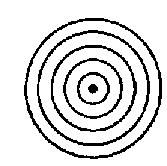
\includegraphics[scale=0.3]{atomA.jpg} \\ a)
\end{center}
\end{minipage}
\hfill
\begin{minipage}{0.33\linewidth}
\begin{center}
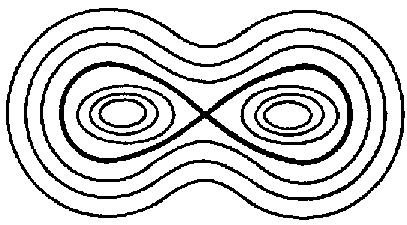
\includegraphics[scale=0.2]{atomB.jpg} \\ б)
\end{center}
\end{minipage}
\hfill
\begin{minipage}{0.98\linewidth}
\begin{center}
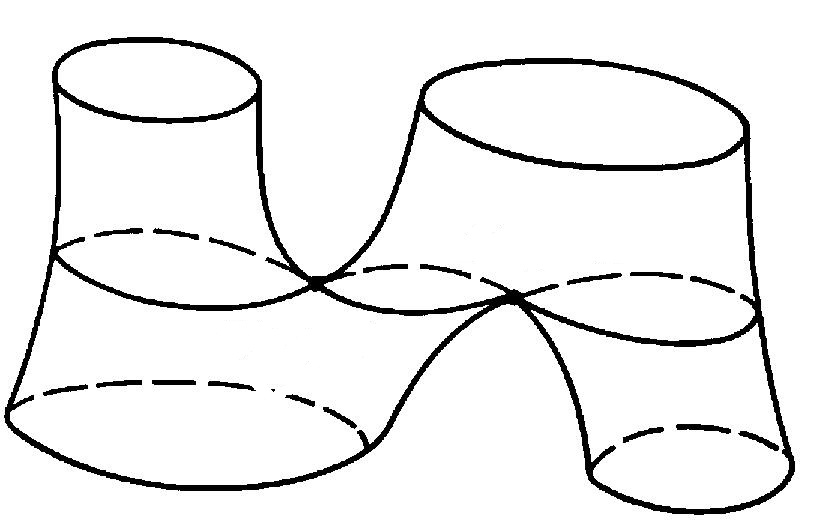
\includegraphics[scale=0.2]{unstable.jpg} \\ в)
\end{center}
\end{minipage}
\caption{\small{Двумерные базы 3-мерных окрестностей особых слоёв слоения Лиувилля на неособом изоэнергетическом многообразии: а --- типа $A$; б --- типа $V_2=B$; в --- пример 4-мерной перестройки торов Лиувилля с несогласованными ориентациями критических окружностей (показана зависимость двумерной базы от уровня энергии h). Трёхмерная (соотв. четырёхмерная) бифуркация получается в результате умножения двумерной базы (при каждом значении h) на окружность.}}
\end{figure}

% Оформление списка литературы
\smallskip \centerline {\bf Литература} \nopagebreak

1. {\it Кантонистова Е. О.} Топологическая классификация интегрируемых гамильтоновых систем на поверхностях вращения в потенциальном поле.
Матем.сб.,2016, том 207, №3, с. 47--92.

2. {\it Болсинов А. В., Фоменко А. Т.} Интегрируемые гамильтоновы системы. Геометрия, топология, классификация. Ижевск: Издательский дом <<Удмуртский университет>>, 1999.

%\end{document} 

\begin{center}
    {\bf ������������� ����������� ��������� ��������\\ � ��������ͨ���� ������������\footnote{������ ��������� ��� ���������� ��������� ���� � ������������� ���������� ��������� � ������ �������� �������  � 18-41-160029.
������ ���������� ���� (������ � 19-31-90063).}}\\

    {\it �.�. �����������, �.�. ��������, �.�. ��������, �.�. ��������}

    (������; {\it diana.korosteleva.kpfu@mail.ru})
\end{center}

\addcontentsline{toc}{section}{����������� �.�., �������� �.�., �������� �.�., �������� �.�.}


����������� ���������� ���������������� ������ �� ����������� �������� � ������� ����������� ��������� �������,
����������� ���������� ����������� ��������� ���������� ������� ���������� �������� � �������������� ������������.
�������������� ������������ ��������� ������� ���������� ��������.
��� ������ ����� ����������� ������������������ ������������� �������������� ����������� ��������
� ���������� ������ �� �������������.
������������������ ����������� �������� ������������� ������������� �������
����������� �������.
� ��������� ������ ��������� �������� ����������� �������� � ����������� �������
��� ��������� ���������� ��������������� �����������.
�������� ���������������� ������ �� ����������� �������� ����������������
�������� ������ ������ �������� ��������� �� ����������� �����.
����������� �������� ����������� ����������� ��������
� ����������� ������� � ����������� �� ���� �����.
���������� ���������� ��������� � �������� ���������� �����~[1--3].



% ���������� ������ ����������
\smallskip \centerline {\bf ����������} \nopagebreak

1. {\it ��������~�.�.}
���������� ������ �� ����������� ��������. ����������� ������.
Saarbr\"ucken: LAP Lambert Academic Publishing, 2011. 256 �.

2. {\it ��������~�.�.}
������������� ���������� ������������ ����� � ������������ ������������
// ���������������� ���������. 2015. �. 51,
� 7. �. 937--950.

3. {\it ��������~�.�.}
����������� ��������� ������� � ������ �������������� ������
// ���������������� ���������. 2017. �. 53,
� 3. �. 418--432.








\begin{center}
    {\bf � ���������� ������������ ������ ���� ��� ����������� ��������� �������� � ������� �����������}

    {\it �.�. ������, �.�. ��������, �.�. ��������}

    (�������; ��� ��. �.�. ����������; {\it jancd@inbox.ru})
\end{center}

\addcontentsline{toc}{section}{������ �.�., �������� �.�., �������� �.�.}


� ��������� ������������ $E$ � ������ $||*||_E$ ��cc����������� ���������

\begin{equation}\label{eq_lin_operator}
	\frac{\partial^{1+\alpha} u(t)}{\partial t^{1+\alpha}} = Au(t), \ \ \ t \geqslant 0
\end{equation}

��� $A$  - �������� ��������� �������� � �������� ����������� $D(A) \subset E$ � �������� �������� $R(A)$.

\begin{equation}\label{Green_Eq}
        \frac{\partial^{1+\alpha}u(t,x)}{\partial t^{1+\alpha}} = \frac{1}{\Gamma(1-\alpha)} \int\limits_0^t \frac{u''(s)ds}{(t - s)^{\alpha}}; \ \ \ \alpha \in (0, 1)
\end{equation}
 - ������� ����������� � ������ ������.
\vspace{3mm}


��������������� ������ � ���������� ������� ��������� \ref{eq_lin_operator}, ��������������� ��������

\begin{equation}\label{Koshi_uslovie}
	u(0) = u_0, \ u'(0) = 0
\end{equation}

\begin{definition}
	�������� ��������� \ref{eq_lin_operator} ���������� ��������-������� $u(t)$ �� ���������� � $D(A)$, ��� ������� ������������ ����������� \ref{Green_Eq} � ��������������� ��������� \ref{eq_lin_operator}
\end{definition}

\begin{definition}
	�������� ��������� \ref{eq_lin_operator} ��������������� �������� \ref{Koshi_uslovie}, ��� $u_0 \in D(A), u_1 \in D(A)$, ���������� �������� ������ ����.
\end{definition}

\begin{definition}
	������ \ref{eq_lin_operator} - \ref{Koshi_uslovie} ����� �������� ����������-����������, ���� ��� �� ������� ����������� ������
	\begin{equation}\label{ocenka}
		||u(t)||_E \leq M||u_0||_E,
	\end{equation}
	��� ��������� $M$ �� $t$ � $u_0$ �� �������.
\end{definition}
��� ��������� $A$, ��������� ���������� $D=d^2/dx^2$, ��������� \ref{eq_lin_operator} ��������������� �. �������� [7].
\vspace{3mm}


� ��������� ��������� ������������
	\begin{Theorem}
		���� �������� $A$ �������� ������������ ���������� ������-����������� ������� ������� $C(t,A)$ � �������
		\begin{equation}
			||C(t,A)||_E \leq M,
		\end{equation}
		�� ������ ���� \ref{eq_lin_operator} - \ref{Koshi_uslovie} ����������-��������� � �� ������� ����� ���
		\begin{equation}
			u(t) = \int\limits^{\infty}_0 I^{(1-\alpha)}_t (h_{\alpha}(t, \xi) C(\xi, A)u_0 d\xi,
		\end{equation}
	\end{Theorem}
	��� $I^{(1-\alpha)}f(t)$ - ������� �������� �������-�������,
	$$
		h_\alpha(t,s) = \frac{1}{2\pi i} \int\limits^{\sigma + i\infty}_{\sigma - i \infty} e^{tp-\xi p^{\alpha}} dp
	$$ --- ������� ������
	� ����������� ������ \ref{ocenka}
	
\smallskip \centerline {\bf ����������} \nopagebreak

1. {\it ������ �.} �������������� ������ // �. ������ - ������������ ���, ������ 1967, �. 357.

2. {\it ��������� ��.} ���������� �������� ���������� � �� ����������. ����: ���� �����, 1989. 347 �.

3. {\it ����� �.�.} �������� ���������������� ��������� � ��������� ������������, �.: ����� 1967. -464 �.

4. {\it ������ �.�.} ����������� ������ / ������� ������� ������-�������������� ���������� ���-�� "����� �., 1973. - 544 �.

5. {\it Kurepa S.} Semigroups  and cosine functions. Lecture Notes in Math, vol 948 Berlin, Springs, 1982. - p. 47 - 72.

6. {\it ����� �.�.} ��������� � ����������� �������� ������� � ��������� �� ���������� // �.�. ����� / �.�. ������ / �.�. �������

7. {\it Mainardi F.} ��������� ��������� ��������-�����. ����������� � ��������� �����������, ���. 38, �1-2, 1995

8. {\it ������ �.�.,. ������ �.�,. ������ �.�} "����������� �������-������� � ��������� ������". ���, 2019,�.486 �5, �.531-536.




\setcounter{equation}{0}
\setcounter{Theorem}{0}
\setcounter{definition}{0}

\begin{center}
{\bf Костин В.А., Костин А.В.\\ Экспоненциальные косинус
оператор-функции и их связки}
\end{center}
\addcontentsline{toc}{section}{Костин В.А., Костин А.В.}



Пусть $\mathbb{R}=(-\infty,\infty)$, $E$~--- банахово пространство,
$C(t)$--- операторная косинус-функция класса $C_0$ (КОФ).

Это означает, что выполняются соотношения:\\
$(i)\hspace{10mm}C(t+s)+C(t-s)=2C(t)C(s),\hspace{10mm}t,s\in\mathbb{R};$\\
$(ii)\hspace{10mm}C(0)=I$--- тождественный оператор в $E$;\\
$(iii)\hspace{10mm}\lim\limits_{t\to 0}\|C(t)\varphi-\varphi\|_E=0$
для всех $\varphi\in E$.

Оператор $A=C''(0)$ называется производящим оператором (генератором)
с областью определения $\overline{D}(A)=E$.

{\bf Определение 1 [1]}. Если КОФ представима в виде
$$C(t)=\frac12[\exp(tA)+\exp(-tA)],\hspace{10mm}t\in\mathbb{R},\eqno{(1)}$$
где $\exp(tA)$--- однопараметрическая группа преобразований с
генератором $A$, то она называется экспоненциальной косинус
оператор"=функцией с генератором $A^2$.

Известно (см. [2]), что КОФ является экспоненциальной только тогда,
когда операторы $A$ и $-A$ являются генераторами сильно непрерывных
полугрупп в $E$.

{\bf Определение 2.} Если $C_1(t)$ и $C_2(t)$ экспоненциальные
косинус оператор"=функции в $E$, коммутирующие между собой, то
конструкцию $$C_1(t)\ast
C_2(t)=\frac12[\exp(tA_1)\exp(tA_2)+\exp(-tA_1)\exp(-tA_2)]$$ будем
называть связкой косинус"=функций $C_1(t)$ и $C_2(t)$.

{\bf Утверждение.} Если $C_1(t)$~--- экспоненциальная
косинус"=фу\-н\-к\-ция с генератором $A_1^2$, а $C_2(t)$~--- с генератором
$A_2^2$, то их связка является экспоненциальной косинус"=функцией с
генератором $(A_1+A_2)^2$.

{\bf Литература}

1. Васильев В.В. Полугруппы операторов, косинус оператор"=функции и
линейные дифференциальные уравнения// В.В. Васильев, С.Г. Крейн,
С.И. Пискарев/ Итоги науки  техники. Мат. анализ., Т. 28, М.: 1996,
с. 87--202.

2. Костин В.А. Абстрактные сильно непрерывные пары
тригонометрических групп преобразований// В.А. Костин/ № 829--80
Деп. Воронеж.--- 1980, 20 с.


%\documentclass[a5paper, 12pt, openbib]{report}
%\usepackage[cp1251]{inputenc}
%\usepackage[english, russian]{babel}
%\usepackage[colorlinks=true, urlcolor=blue]{hyperref}
%\usepackage{graphicx}
%\usepackage[tmargin=1.75cm,
%            bmargin=2.1cm,
%            lmargin=1.75cm,
%            rmargin=1.75cm]{geometry}
%
%\righthyphenmin=2
%
%\clubpenalty=10000
%\widowpenalty=10000
%
%\begin{document}

\begin{center}
    {\bf �������� ������� ��� ��������� ���������}

    {\it �.�. �������}

    (�������; {\it tata@rambler.ru})
\end{center}

\addcontentsline{toc}{section}{������� �.�.}

	�������������� ������ ��������� �������� � ��������� ������������� ������, �������������� ���������� ��������� ����� ��������� ��� [1]:
 $$
(1+e\cos(\nu))\-
2e\sin(\nu)+\frac{d\delta}{d\nu}+\mu\sin(\delta)-4e\sin(\nu) =0,
\eqno{(1)}
 $$
��� �������� $e$ --- �������������� ������, $\mu$ --- ��������,
��������������� ������������� ����� ��������, $\nu$ ---
������� (��������) ���������� ������ ���� ��������, $\delta$ --- ����
����� ��������� �������� � ���� ��������� ��������.


� ������  $e\neq0$ �  $\mu\neq1$ ��������� (3) �� �������������, ������� ��� ��� ������� ������������ ������������ ������, �������� ����� ��������-������. ��� ��� ����������  ���� ��������  [3], ��� ��������� ��������� �������� ������������, ��� ������
������������� ��������� $(1+e\cos(\nu))$, ��� ��������� �� ������� ��������� (1) ����������
 ���������� ������-�������� ��� �����������
����������� ��������
 $$
V(q)=\int\limits_{0}^{2\pi}L(\dot{q},q)dt,
 $$
� ������������ $L(\dot{q},q)$:
 $$
\frac{\dot{q^2}}{2}(1+e\cos(\nu))^2+(1+e\cos(\nu))4eq\sin(\nu)+
(1+e\cos(\nu))\mu\cos(q).
 $$





 ����� �������� ������ ���������� ��������� ��������� � ������������ �������� �������. ������������ ����������
�������� ������� �������������� �� ������ �������������
���������-����� � �������� ��������, � ������� ���������� ������ ������������ ������ � ����� ��������
����������� ������� $V$:
$$
 \frac 1{2\pi} \int\limits
_0^{2\pi}\left((1+\varepsilon\,e_1(t))^2 \ \frac{\dot{x}^2}{2} +
(1+\varepsilon\,e_1(t))( \mu
 \cos (x)+4\varepsilon x e_2(t))\right) dt.
 $$
 ���������� ���������� ������������ ��������, ����������� ������� �������� ������� �  ����� ��������� ���������.
$$
W(\xi_0, \xi_1, \xi_2,\mu,
\varepsilon)=\inf V (\xi_0 + \xi_1 e_{1} + \xi_2e_{2} +v),
 $$
 ��� $  e_{1}=\sqrt{2}\cos(t),  e_{2}=\sqrt{2}\sin(t).$

 � ����� � ��������� ����������� ������������ ������� � ������� ���������� ������� ����� ��������� �������� ������� �������� ������� � �������� ������������ ������.
 ��� ������������ ����������
���������� � �������  ��������� ������������ �����������
���������. ��������� ������� �������� ������ ����������� ������, ����� ���������� ������������ ��� ��������� ��������.
 ������������ ��������� �������  �������� ���������, ����������� ��-��
����, ��� ���������� �������� ����������� ������������
������ �������. ������� $\xi_2=0$ ����� �������� ��������� �������� �����������.


��������  ������������ ����������� ������������ ����� �������
�������������� ����������� �������� ������� ��� ��������� ��������� ��� ���� ��������� ��������� ���������:

\begin{center}
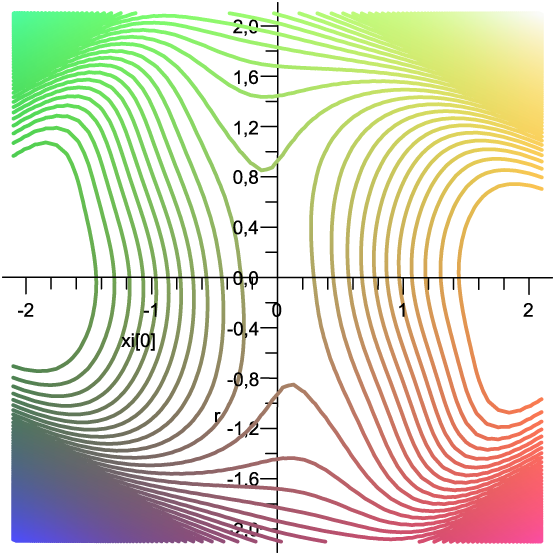
\includegraphics[width=0.3\textwidth,angle=0]{e01.png} \ \
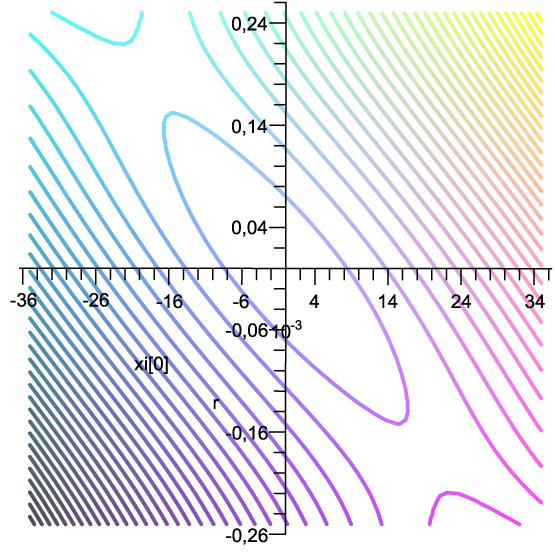
\includegraphics[width=0.3\textwidth,angle=0]{e02.png}

���. 1. ��������� ����� �������  �������� �������  ��� ��������� ��������� ��� {$\mu
= 1.1\,, \ \varepsilon=0.2\,;$ \ $\mu = 1.05\,, \
\varepsilon=0.1\,. $}

\end{center}

%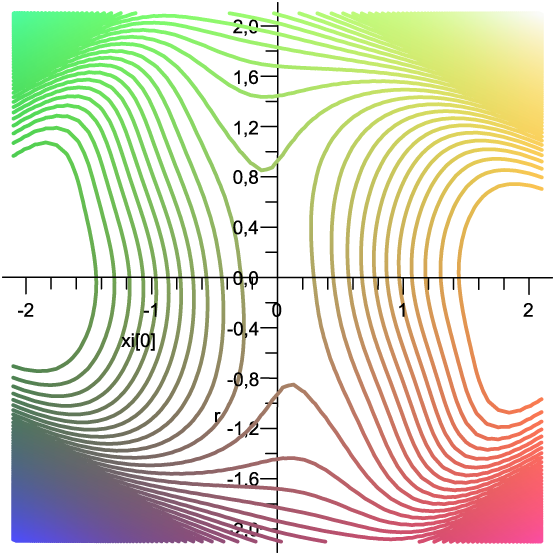
\includegraphics[width=0.3\textwidth,angle=0]{e01.eps} \ \
%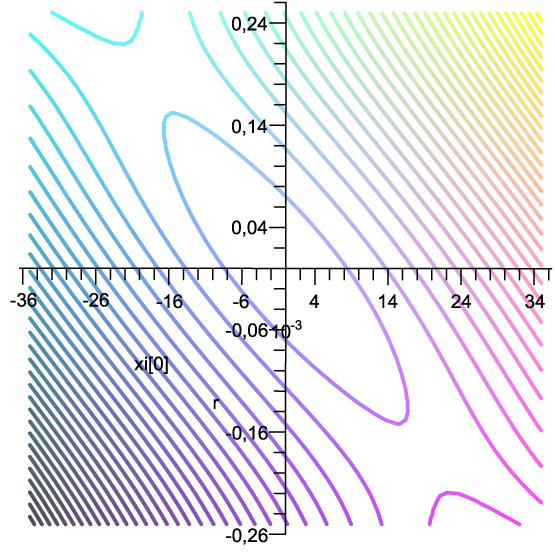
\includegraphics[width=0.3\textwidth,angle=0]{e02.eps}

%\includegraphics[width=0.3\textwidth,angle=0]{e01-d.eps} \ \
%\includegraphics[width=0.3\textwidth,angle=0]{e02-d.eps}

%\includegraphics[width=0.3\textwidth,angle=0]{e01-dd.eps} \ \
%\includegraphics[width=0.3\textwidth,angle=0]{e02-dd.eps}



% ���������� ������ ����������
\smallskip \centerline {\bf ����������} \nopagebreak

1. �������� �.� �������� �������������� �������� ������������ ������ ����.
-- �.: �����, 1965. -- 416 �.


2. ������� �.�. ����������� ���������� �������� ������� � ������ �
������������� �������� ������������ ��������� // �������
������������ ���������������� ������������. �����: ������.
����������. \No 1. 2011 -- �. 181-186.


3. ������� �.�. � ��������� ������������� ������� ���������  ��������� �������� � ��������� ���������// �.�. ������� , �.� �������� / ������� ������������ �������
������������ ���������������� ������������. �����: ������.
����������. \No 1. 2018 -- �.99-114.



%\end{document} 


\begin{center}

{\bf ДОСТАТОЧНЫЕ УСЛОВИЯ СОГЛАСОВАНИЯ ХАРАКТЕРИСТИЧЕСКИХ ВТОРЫХ
ПРОИЗВОДНЫХ ГРАНИЧНОГО РЕЖИМА С НАЧАЛЬНЫМИ УСЛОВИЯМИ И ОДНОМЕРНЫМ
ВОЛНОВЫМ УРАВНЕНИЕМ ДЛЯ ГЛАДКИХ РЕШЕНИЙ}  % Заголовок прописными буквами

{\it Ф.Е. Ломовцев, К.А. Спесивцева} 

(Минск; {\it lomovcev@bsu.by,
ksenia.spesivtseva@gmail.com})

\end{center}
\addcontentsline{toc}{section}{Ломовцев Ф.Е., Спесивцева К.А.}

Для первой четверти плоскости ~$\dot{G}_\infty=]0,+\infty[ \times
]0,+\infty[$ в задаче
$$
u_{tt}(x,t) + (a_1 - a_2)u_{xt}(x,t) - a_1a_2 u_{xx}(x,t) =
f(x,t), \, (x,t) \in \dot{G}_{\infty}, \eqno(1)
$$
$$
u(x,t)\lvert_{t=0} = \varphi(x), \, u_t(x,t)\lvert_{t=0} =
\psi(x), \, x>0, \eqno(2)
$$
$$[\zeta(t)u_{tt}+\xi(t)u_{xt}+\theta(t)u_{xx}+\alpha(t)u_t+\beta(t)u_x+\gamma(t)u]\lvert_{x=0}=\mu(t),
\,t>0, \eqno(3)
$$
нижними индексами функции $u$ обозначены её частные производные
соответствующих порядков по указанным в индексах переменным, ~$a_1
> 0$, ~$a_2 > 0,$  ~$\zeta,\, \xi,\, \theta,\,
\alpha,\, \beta,\, \gamma$ -- заданные функции от ~$t$ и ~$ f, \,
\varphi,\, \psi, \, \mu$ -- заданные функции своих переменных $x$
и $t$. Впервые зависящие от времени $t$ коэффициенты в граничных
режимах (3) для уравнения колебаний струны (1) при $a_1=a_2$
появились в [1].

Уравнение (1) имеет характеристики $x-a_1t=C_1$, $x+a_2t=C_2,$
$\forall$  $C_1,\,C_2\in \mathbb{R}=]-\infty,+\infty[$.
Характеристика $x=a_1t$ является критической для уравнения (1)
[2]. Она делит первую четверть плоскости $G_{\infty}=[0,+\infty[
\times [0,+\infty[$ на два множества $G_{-}$ и $G_{+}$ [2]. Под
$C^{k}(\Omega)$ понимается множество всех $k$ раз непрерывно
дифференцируемых функций на подмножестве $\Omega\subset
\mathbb{R}^2$ и $C^0(\Omega)=C(\Omega)$. В случае
нехарактеристических вторых производных в граничном режиме (3)
критерий корректности задачи (1)--(3) для классических решений
$u\in C^{2}(G_{\infty})$ найден в [2]. Для характеристических
вторых производных в (3) для ограниченной струны нужны критерии
корректности этой задачи для более гладких решений $u\in
C^{m}(G_{\infty}),\,m\geq 2.$

{\bf\textit{Определение.} } Гладким $m$ раз непрерывно
дифференцируемым решением начально-граничной задачи (1)--(3)
называется функция ~$u\in C^{m}(G_{\infty})$, где $m=2,3,4,\,...$,
удовлетворяющая уравнению (1) в обычном смысле, а начальным (2) и
граничному (3) условиям в смысле пределов соответствующих
выражений от её значений $u(\dot{x},\dot{t})$ во внутренних точках
$(\dot{x},\dot{t})\in \dot{G}_\infty$ для всех указанных в них
граничных точек $x$ и $t$.

Для решений $u \in C^{m+1}({G}_\infty)$  задачи (1)--(3) на
<<единицу>> большей гладкости верны следующие условия
согласования.

\textbf{Теорема.} {\it Пусть в граничном режиме (3) коэффициенты
имеют гладкость порядка $m$:
$\zeta,\,\xi,\,\theta,\,\alpha,\,\beta,$ $\gamma\in
C^m[0,+\infty[,$ первые производные берутся не вдоль: $a_1
\alpha(t)\neq\beta(t),\, t\in[0,+\infty[,$ а вторые производные --
вдоль критической характеристики уравнения (1):
$a_1^2\zeta(t)-a_1\xi(t)+\theta(t) \equiv 0,\,t\in[0,+\infty[.$
Если начально-граничная задача (1)--(3) имеет решение $u\in
C^{m+1}(G_\infty)$, то для правой части $f \in C^{m-1}(G_\infty)$,
начальных $\varphi \in C^{m+1}[0,+\infty[,$ $\psi \in
C^{m}[0,+\infty[$ и граничного
 $\mu \in C^{m-1}[0,+\infty[$ данных верны условия согласования}
$$
Y_{k+1} \equiv \sum_{i=0}^{k} Z_{i\,k} = \mu^{(k)}(0), \,\, k \in
[0, m-1],\,\, m\ge2, \eqno(4)
$$
{\it где слагаемые этой суммы соответственно равны}
 $$
Z_{0\,k} \equiv \zeta^{(k)}(0)
\big[f(0,0)+(a_2-a_1)\{\psi^{(1)}(0)+a_1\varphi^{(2)}(0)\}\big]+\xi^{(k)}(0)\times
$$
$$
\times\big[\psi^{(1)}(0) + a_1\varphi^{(2)}(0) \big] +
\alpha^{(k)}(0)\psi(0) + \beta^{(k)}(0)\varphi^{(1)}(0) +
\gamma^{(k)}(0)\varphi(0),
$$
$$
Z_{1\,k} \equiv k \Big\lbrace \zeta^{(k-1)}(0)
[f^{(0,1)}(0,0)+(a_2-a_1)f^{(1,0)}(0,0)+a_2(a_2-a_1)\times
$$
$$
\times\{\psi^{(2)}(0)+a_1\varphi^{(3)}(0)\}] +\xi^{(k-1)}(0)
[f^{(1,0)}(0,0)+a_2\{\psi^{(2)}(0)+a_1\varphi^{(3)}(0)\}]+
$$
$$ +
\alpha^{(k-1)}(0) [f(0,0)+(a_2-a_1)\psi^{(1)}(0) + a_1
a_2\varphi^{(2)}(0)] +
$$
$$
+
\beta^{(k-1)}(0)\psi^{(1)}(0)+\gamma^{(k-1)}(0)\psi(0)\Big\rbrace,
$$
$$
Z_{i\,k} \equiv \frac{k\,!}{i\,!\,(k-i)\,!}\Bigg< \zeta^{(k-i)}(0)
\Bigg\lbrace \sum _{s=1}^{i+1} \rho_{s-1} f^{(s-1,i-s+1)}(0,0)-
$$
$$
- a_1^2\sum _{s=1}^{i-1} \rho_{s-1}
f^{(s+1,i-s-1)}(0,0)+\Big[\eta_{i+1}-a_1^2\eta_{i-1}\Big] \varphi
^{(i+2)}(0) +
$$
$$
+\Big[\rho_{i+1}-a_1^2\rho_{i-1}\Big] \psi ^{(i+1)}(0)
\Bigg\rbrace +\xi^{(k-i)}(0) \Bigg\lbrace \sum _{s=1}^i \rho_{s-1}
f^{(s,i-s)}(0,0)+
$$
$$ + a_1\sum _{s=1}^{i-1}
\rho_{s-1} f^{(s+1,i-s-1)}(0,0)+\Big[\eta_{i}+a_1\eta_{i-1}\Big]
\varphi ^{(i+2)}(0)+
$$
$$ +
\Big[\rho_{i}+a_1\rho_{i-1}\Big] \psi ^{(i+1)}(0)\Bigg\rbrace +
\alpha^{(k-i)}(0) \sum _{s=1}^i \rho_{s-1} f^{(s-1,i-s)}(0,0)+
$$
$$
+\beta^{(k-i)} (0) \sum _{s=1}^{i-1}\rho_{s-1}
f^{(s,i-s-1)}(0,0)+\Big[\eta_i\alpha^{(k-i)}(0)+
\eta_{i-1}\beta^{(k-i)}(0) \Big]\times
$$
$$
\times\varphi ^{(i+1)}(0) + \Big[\rho_i\alpha^{(k-i)}(0)+
\rho_{i-1}\beta^{(k-i)}(0) \Big]\psi ^{(i+1)}(0)+
$$
$$
 + \gamma^{(k-i)}(0)\Bigg\lbrace \sum
_{s=1}^{i-1} \rho_{s-1} f^{(s-1,i-s-1)}(0,0)+\eta_{i-1} \varphi
^{(i)}(0)+
 \rho_{i-1} \psi ^{(i-1)}(0) \Bigg\rbrace \Bigg>,
 $$
 {\it где $i \in [2, k], \, k \in [2, m-1],$ и
$\rho_{j}$ и $\eta_{j}$ находятся реккурентно}
 $$
 \rho_{j}=(a_2-a_1)\rho_{j-1}+a_1 a_2\rho_{j-2}, \,j\geq 2,\, \rho_{0}=1, \, \rho_{1}=a_2-a_1,
 $$
 $$
 \eta_{j} = (a_2-a_1)\eta_{j-1}+a_1 a_2\eta_{j-2}, \,j\geq 2,\,\, \eta_0 = 0, \, \eta_{1} = a_1 a_2.
 $$


 Здесь справа сверху над коэффициентами ~$\zeta,\, \xi,\,
\theta,\, \alpha,\, \beta,\, \gamma$, начальными $\varphi,\,\psi$
и граничным $\mu$ данными задачи цифрой в круглых скобках
обозначены порядки производных по $x$ или $t.$ Аналогично
обозначены в круглых скобках через запятую соответственно порядки
частных производных по $x$ и $t$ от правой части $f.$

{\bf Идея доказательства.} Доказательство осуществляется методом
математической индукции.  Чтобы получить условие (4) при $k=0$ в
равенстве (3) полагаем $t=0$ и используем правую часть уравнения,
начальные данные и характеристичность вторых производных. Для
получения условий (4) при $0<k\leq m-1$ равенство (3)
дифференцируется $k$ раз по $t$, вычисляются значения производных
от решения $u$ при $x=0, \, t=0$ с помощью начальных условий (2),
уравнения (1) и характеристичности вторых производных.


\smallskip \centerline{\bf Литература}\nopagebreak

1. \textit{Ломовцев Ф.Е.}  {О необходимых и достаточных условиях
однозначной разрешимости задачи Коши для гиперболических
дифференциальных уравнений второго порядка с переменной областью
определения операторных коэффициентов./ Ф.Е.~Ломовцев~//
Дифференц. уравнения.~--- 1992.~--- Т. 28, № 5.~--- С. 873--886.}


2. \textit{Ломовцев Ф.Е.} {Нехарактеристическая смешанная задача
для одномерного волнового уравнения в первой четверти плоскости
при нестационарных граничных вторых производных. / Ф.Е.~Ломовцев,
В.В~Лысенко~// Веснiк Вiцебскага дзяржаунага унiверсiтэта, № 3
(104),~--- 2019.~--- С.~5--17.}







\begin{center}
    {\bf ДОСТАТОЧНЫЕ УСЛОВИЯ СОГЛАСОВАНИЯ ХАРАКТЕРИСТИЧЕСКОЙ КОСОЙ
ПРОИЗВОДНОЙ ГРАНИЧНОГО РЕЖИМА С НАЧАЛЬНЫМИ УСЛОВИЯМИ И ОДНОМЕРНЫМ
ВОЛНОВЫМ УРАВНЕНИЕМ ДЛЯ ГЛАДКИХ РЕШЕНИЙ}

    {\it Ф.Е. Ломовцев, Е.В. Устилко}

    (Минск; {\it lomovcev@bsu.by, ustilko@tut.by})
\end{center}

\addcontentsline{toc}{section}{Ломовцев Ф.Е., Устилко Е.В.}

Выведены достаточные условия согласования для смешанной задачи с
характеристической косой производной в граничном режиме в первой
четверти плоскости ~$\dot{G}_\infty=]0,+\infty[ \times
]0,+\infty[$ :
$$
u_{tt}(x,t) + (a_1 - a_2)u_{xt}(x,t) - a_1a_2 u_{xx}(x,t) =
f(x,t), \, (x,t) \in \dot{G}_{\infty}, \eqno(1)
$$
$$
u(x,t)\lvert_{t=0} = \varphi(x), \, u_t(x,t)\lvert_{t=0} =
\psi(x), \, x>0, \eqno(2)
$$
$$[\alpha(t)u_t+\beta(t)u_x+\gamma(t)u]\lvert_{x=0}=\mu(t),
\,t>0, \eqno(3)
$$
где нижними индексами функции $u$ обозначены её частные
производные соответствующих порядков по указанным в индексах
переменным, постоянные~$a_1
> 0$, ~$a_2 > 0,$ коэффициенты~$\alpha,\, \beta,\, \gamma$ -- заданные функции переменной ~$t,$
$a_1\alpha(t)=\beta(t),\, t>0,$ и исходные данные~$ f,
\,\varphi,\, \psi, \, \mu$ -- заданные функции своих переменных
$x$ и $t$.

Уравнение (1) имеет характеристики $x-a_1t=C_1$, $x+a_2t=C_2,$
$\forall$  $C_1,\,C_2\in \mathbb{R}=]-\infty,+\infty[$.
Характеристика $x=a_1t$ является критической для уравнения (1) и
делит множество $G_{\infty}=[0,+\infty[ \times [0,+\infty[$ на два
подмножества $G_{-}$ и $G_{+}$ [1]. Под $C^{k}(\Omega)$ понимается
множество всех $k$ раз непрерывно дифференцируемых функций на
подмножестве $\Omega\subset \mathbb{R}^2$ и
$C^0(\Omega)=C(\Omega)$. Критерий корректности смешанной задачи
(1)--(3) для простейшего уравнения колебаний полуограниченной
струны (1) при $a_1=a_2$ с характеристической косой производной
граничного режима (3) во множестве классических решений $u\in
C^{2}(G_{\infty})$ установлен в [1]. Работа [2] свидетельствует о
том, что в случае характеристической косой производной граничного
режима (3) для уравнения колебаний ограниченной струны нужны
критерии корректности этой вспомогательной смешанной задачи
(1)--(3) для более гладких решений $u\in C^{m}(G_{\infty}),\,m\geq
2.$

{\bf\textit{Определение.} } Гладким $m$ раз непрерывно
дифференцируемым решением начально-граничной задачи (1)--(3)
называется функция ~$u\in C^{m}(G_{\infty})$, где $m=2,3,4,\,...$,
удовлетворяющая уравнению (1) в обычном смысле, а начальным
условиям (2) и граничному режиму (3) в смысле пределов
соответствующих выражений от её значений $u(\dot{x},\dot{t})$ во
внутренних точках $(\dot{x},\dot{t})\in \dot{G}_\infty$ для всех
указанных в них граничных точек $x$ и $t$.

Для решений $u \in C^{m+1}({G}_\infty)$  задачи (1)--(3) на
<<единицу>> большей гладкости нами найдены условия согласования.
Для этих решений из (1)--(3) вытекают очевидные требования
гладкости
$$
f \in C^{m-1}(G_\infty), \, \varphi \in C^{m+1}[0, +\infty[, \,
\psi \in C^{m}[0, +\infty[, \, \mu \in C^{m}[0, +\infty[.
 \eqno{(4)}
 $$

Для получения первого условия согласования в равенстве (3)
полагаем $t=0$ и вычисляем значения слагаемых его левой части,
используя условия (2) и характеристичность первых производных
$$
 \alpha(0)[\psi(0)+a_1\varphi^{(1)}(0)]+\gamma(0)\varphi(0) = \mu(0).\eqno(5)
$$
Второе условие согласования граничного режима (3) с начальными
условиями (2) и уравнением (1) находится, полагая $t=0$ в первой
производной по $t$ от равенства (3) и вычисляя значения
соответствующих производных от решения $u$ при $x=0, \, t=0$ с
помощью начальных условий (2) при $x=0$, уравнения (1) при $x=0,
\, t=0$ и характеристичности первых производных
$$
 \alpha^{(1)}(0)[\psi(0)+a_1\varphi^{(1)}(0)]+\gamma^{(1)}(0)\varphi(0)+
$$
$$
 + \alpha(0)\big\langle a_2[\psi^{(1)}(0)+a_1\varphi^{(2)}(0)] + f(0,0)\big\rangle + \gamma(0)\psi(0) = \mu^{(1)}(0).
 \eqno(6)
$$

Аналогичным образом выводятся остальные условия согласования
граничного режима с начальными условиями и уравнением.

\textbf{Теорема.} {\it Пусть в граничном режиме (3) с
коэффициентами $\alpha,\,\beta,$ $\gamma\in C^m[0,+\infty[$ косая
производная является характеристической, т.е. она направлена вдоль
критической характеристики уравнения (1): $a_1 \alpha(t) =
\beta(t),\, t\in[0,+\infty[.$ Если смешанная задача (1)--(3) имеет
решение $u\in C^{m+1}(G_\infty)$, то для исходных данных $f,\,
\varphi, \,\psi,\, \mu$ из (4) справедливы условия согласования
(5), (6) и}
 $$
\alpha^{(q)}(0)[\psi(0)+a_1\varphi^{(1)}(0)]+\gamma^{(q)}(0)\varphi(0)
+
 $$
 $$
+ q\bigg\{\alpha^{(q-1)}(0)\bigg\langle
a_2[\psi^{(1)}(0)+a_1\varphi^{(2)}(0)]+f(0,0)\bigg\rangle+\gamma^{(q-1)}(0)\psi(0)\bigg\}+
 $$
 $$
+\sum _{i=2}^{q} \frac{q\,!}{i\,!\,(q-i)\,!}\Bigg\{
\alpha^{(q-i)}(0)\Bigg\langle
a_2^{i}[\psi^{(i)}(0)+a_1\varphi^{(i+1)}(0)]+
$$
$$
 + \sum _{j=0}^{i-1}
a_2^{j}
f^{(j,\,i-j-1)}(0,0)\Bigg\rangle+\gamma^{(q-i)}(0)\Bigg\langle
 (-a_1)^{i-1} \psi ^{(i-1)}(0)+
$$
$$
+\,a_2\,\frac{a_2^{i-1}-(-a_1)^{i-1}}{a_1+a_2}\,[\psi^{(i-1)}(0)+a_1\varphi^{(i)}(0)]+
 $$
 $$
 +\sum _{k=0}^{i-2}\,
\frac{a_2^{k+1}-(-a_1)^{k+1}}{a_1+a_2}\, f^{(k,\,i-k-2)}(0,0)
\Bigg\rangle\Bigg\}=\mu^{(q)}(0),\,q=\overline{2,m}.\eqno(7)
 $$


 Здесь справа сверху над коэффициентами ~$\alpha,\, \beta,\, \gamma$, начальными $\varphi,\,\psi$
и граничным $\mu$ данными этой задачи цифрой в круглых скобках
обозначены порядки производных по $x$ или $t$. Аналогичным образом
в круглых скобках через запятую обозначены соответственно порядки
частных производных по $x$ и $t$ от правой части $f$.

{\bf Замечание.} В дальнейшем мы ослабим достаточные условия
согласования (сопряжения) (5)--(7) до необходимых условий таких,
как, например, в [1]. Затем мы их применим для выявления критерия
корректности аналогичной смешанной задачи при характеристических
косых производных на двух концах ограниченной струны без
продолжений данных новым методом <<вспомогательных смешанных задач
для волновых уравнений на полупрямой>> из [3].

\smallskip \centerline{\bf Литература}\nopagebreak

1. \textit{Ломовцев Ф.Е.}  {Необходимые и достаточные условия
вынужденных колебаний полуограниченной струны с первой
характеристической косой производной в нестационарном граничном
условии./ Ф.Е.~Ломовцев~// Весцi НАН Беларусi. Сер. фiз.-мат.
навук.~--- 2016.~--- № 1~--- С. 21--27.}


2. \textit{Ломовцев Ф.Е.} {Смешанная задача для неоднородного
уравнения колебаний ограниченной струны при характеристических
нестационарных первых косых производных на концах. /
Ф.Е.~Ломовцев, Т.С.~Точко~// Веснiк Гродзенскага дзяржаунага
унiверсiтэта iмя Я. Купалы. Серыя 2.~--- 2019.~--- Т. 9, № 2.~---
С.~56--75.}


3. \textit{Ломовцев Ф.Е.} {Метод вспомогательных смешанных задач
для полуограниченной струны. / Ф.Е.~Ломовцев~// Шестые
Богдановские чтения по обыкновенным дифференциальным уравнениям:
матер. Междунар. матем. конф. Минск БГУ. 7--10 дек. 2015 г. в 2 ч.
Минск : ИМ НАН Беларуси.~--- 2015.~--- Ч. 2.~--- С. 74--75.}




\begin{center}
    {\bf  ЗАДАЧА ДИРИХЛЕ ДЛЯ В-ГАРМОНИЧЕСКОГО УРАВНЕНИЯ В ШАРЕ}

    {\it Л.Н. Ляхов, Е.Л. Санина, С.А. Рощупкин}

    (Воронеж,  {\it levnlya@mail.ru, sanina08@mail.ru,} Елец, {\it roshupkinsa@mail.ru})
\end{center}

\addcontentsline{toc}{section}{Ляхов Л.Н., Санина Е.Л., Рощупкин С.А.}



Рассматривается сингулярный дифференциальный оператор Лапласа---Бесселя $\Delta_B$ и $B$-гармоническое уравнение $\Delta_B u=0$ в шаре. Решение граничной задачи Дирихле представлено в виде ряда Лапласа по весовым сферическим функциям. Полученные решения совпадают с решениями классического гармонического уравнения при равенстве нулю всех размерностей операторов Бесселя, входящих в оператор $\Delta_B$.


%Библиография: 13 названий.

%{\bf Ключевые слова}.Весовая сферическая функция, оператор Бесселя, оператор Лапласа---Бесселя на сфере, ряды Лапласа.


  1. {\bf Весовые сферические функции (В-гармоники)}.
Пусть $n$ и $N$ натуральные числа и  $1{\le}n{\le}N$ и пусть\\
$\mathbb{R}^+_N \{x{=}(x',x'')
{=}(x_1\,\ldots\,,x_n,x_{n+1}\,\ldots\,,x_N),\,\,\, x_1{>}0,\ldots,x_n{>}0\}.$ \\
 В $\mathbb{R}_N^+$ рассматривается сингулярный
дифференциальный оператор
$\Delta_B=\sum_{j=1}^nB_j{+}\sum_{i=n+1}^N{\partial^2\over\partial x_i^2},
\,\, B_{x_i}{=}{{\partial^2}\over {\partial x^2}}{+}{\gamma_i\over {x_i}}
{\partial\over{\partial x_i}}\,,\,\, \gamma_i>0.$ Отметим, что обозначение $\Delta_B$ (в настоящее время принятое в мировой литературе)  введено И.А. Киприяновым в 60-х годах прошлого столетия. Из [1] %\cite{Keld}
и книги [2]
%\cite{Kipr}
вытекает, что ограниченные решения уравнений, содержащие оператор $\Delta_B$, надо искать в классе функций $C^2$, четных по каждой из переменных $x_1,\,\ldots\,,x_n$. Такие функции будем называть $x'$-чётными.

%2. {\bf Весовые сферические функции (В-гармоники)}.

{\it Однородный x'-четный многочлен $P_m^\gamma(x)$ порядка $m$,   удовлетворяющий
уравнению $ \Delta_BP_m^\gamma(x)= 0$\,, называется В-гармоничес\-ким.}
{\it Весовой сферической функцией (В-гармоникой)} (далее используется сок\-ра\-ще\-ние --- в.с.ф.)
{\it называется сужение В-гармонического многочлена на сферу:}
$$Y_m^\gamma(\Theta)={P_m^\gamma(x)\over|x|^m}= P_m^\gamma\left(x\over|x|
\right).$$

    Для наших исследований потребуются следующие свойства  в.с.ф., полученные в [3], [4], [5]
%\cite{L1}, \cite{L2}, \cite{L3},
 (см. также книгу [6]).
%\cite{Lya}

 Пусть $S^+_1=\{x:\,|x|=1\}\cap\mathbb{R}_N^+$.

{\bf Ортогональность в.с.ф.}, отвечающих различным порядкам $m$ и $k$
(m,\,k=0,1,2,\ldots),
определяется равенством
$$\int\limits_{S^+_1}Y^\gamma_m(\Theta)\,Y^\gamma_k(\Theta)\,
(\Theta')^\gamma\,dS{=}0, \quad m{\neq}k,\quad Y_0^\gamma(\Theta)=1\,.          \eqno (1)
$$
 \label{posm(1)}  				
где $(\Theta')^\gamma=\prod\limits_{i=1}^n\Theta_i^{\gamma_i}$, ${\cal P}^\gamma_{\Theta'}$ -- многомерный
оператор Пуассона, $C_m^\nu$ --- многочлен Гегенбауэра  и коэффициент $|S^+_1|_\gamma$ определен по формуле
''площади нагруженной сферы'' (см. [6],
с. 20).
Среди в.с. функций данного порядка $m$ в свою очередь можно выбрать
ортогональный базис $Y_{m,k}^\gamma(\Theta)\,,\,\,1{\le}k{\le}d_\gamma(m)$.
В результате получим систему ортогональных в.с. функций
$$\{Y_{m,k}^\gamma(\Theta)\},\quad m{=}0,1,2,\,\ldots\,,\quad k{=}1,2,\,
\ldots\,d_\gamma(m),
 $$
которая  плотна в пространстве непрерывных на $S^+_1$ функций, четных
по каждому аргументу  $x_1,\,\ldots,x_n$ и плотна в $L_2^\gamma(S^+_1)$
и полна в $L_2^\gamma(S^+_1)$.


\textbf{Оценки $D_B$-производных от в.с. функций $Y^\gamma_m(\Theta)$
при $m\to\infty$.}

   Введем обозначение
$$
\left(D_B\right)^\beta_{x'}=
\left\{
\begin{array}{lll}
B^{\beta_i\over2}_{x_i} & , & \beta_i=2k - \hbox{ четное число,} \\
{\partial\over\partial x_i}B^{\beta_i-1\over2}_{x_i} & , & \beta_i=2k{+}1 -
\hbox{ нечетное число,}.
\end{array}\right.
$$
   Имеет место весовая
среднеквадратическая оценка
$$\int\limits_{S^+_N}\left|\left((D_B)^\beta_{x'}\,\,D^\alpha_{x''}\,
P^\gamma_m\right)(x)\right|^2(x')^\gamma\,dS\leqslant C_1 m^{2|\alpha+\beta|}
\Vert Y^\gamma_m\Vert_{L_2^\gamma(S^+_1)}
$$
и равномерная оценка
$$\left|\left(B^\beta_{x'}D^\alpha_{x''}\,P_m^\gamma\right)(x)\right|^2\leqslant C_2m^{2|\alpha+2\beta|{+}N{+}|\gamma|{-}2}
\,|x|^{2m{-}2|\alpha{+}2\beta|}\,\,\Vert
Y^\gamma_m\vert_{L_2^\gamma(S^+_1)}\,\,,
$$% \eqno (1.6.3)
где постоянные $C_1$ и $C_2$ зависят от $n,k,\alpha$ и $\beta$, но не от $m$.


 {\bf Дифференциальное уравнение в.с. функций}:
$$\left(\Delta_B(\Theta)\,Y_m^\gamma\right)(\Theta){=}
m(m{+}N{+}|\gamma|-2)Y_m^\gamma (\Theta)\,.
$$
 Здесь через $\Delta_B(\Theta)$ обозначено сужение  $\Delta_B$ на сферу $S_1^+$ (оператор Бельтрами): $\Delta_B{=}{\partial^2\over\partial r^2}{+}{N{+}|\gamma|{-}1\over r}
{\partial\over\partial r}{+}{1\over r^2}\,\Delta_B(\Theta)$.

  		
	{\bf Ряды  Лапласа по в.с. функциям}.    Справедливы следующие утверждения.
	
  {\it Пусть $f{\in}C^{2l}_{ev}(S^+_1)$ и $a_{m,k}$ и
$b_{m,k}$ коэффициенты Фурье-Лапласа функций $f(\Theta)$ и
$\left(\Delta_B^l(\Theta)\,f\right)(\Theta)$ соответственно по системе в.с.функций. Тогда}
$$a_{m,k}=[m(m+N+|\gamma|-2)]^l\,b_{m,k}.$$

 {\it Если $f{\in}C^{2l}_{ev}(S^+_1)$, то}
$$|a_{m,k}|\le M\,m^{-2l}\,,\quad M{=}\int_{S^+_1}\left|\left(\Delta_B
(\Theta)f\right)(\Theta)\right|^2(\Theta')^\gamma\,dS\,.
$$




\begin{center}
{\bf 2. Задача Дирихле для В-гармонического уравнения в шаре}
\end{center}
%\vskip\baselineskip


Пусть $U=\{x:\,|x|<1\}\cap\mathbb{R_N^+}$. Рассмотрим задачу Дирихле
$$\Delta_B u{=}0,\,\,\, u\left|_{|x|=1}=f(\Theta)\right.\,, u\in C^2(U)\cap C(\overline{U}),\eqno(4)$$
где $\Theta_j=\Theta(\varphi^i),\,\,\,\varphi^i=\left(\varphi_1,...,\varphi_j\right)$ --- сферические координаты точки на замкнутой $n$-полусфере в $\mathbb{R}_N^+$:
  $$
 \left. \begin{array} {l}
\Theta_1=\cos\varphi_1\\
\Theta_2=\sin\varphi_1 \cos\varphi_2\\
\ldots\,\ldots\ldots\ldots\ldots\ldots\ldots\ldots\ldots\ldots\ldots,\,\\
\Theta_{N-1}=\sin\varphi_1 \sin\varphi_2...\sin\varphi_{n-1}\cos\varphi_{n-1},\\
\Theta_N=\sin\varphi_1\sin\varphi_2...\sin\varphi_{n-2}\sin\varphi_{n-1},
\end{array}\right|
\quad\begin{array}{l}
0\leq\varphi_i\leq\pi/2,\\
i=\overline{1,n},\\\\
0\leq\varphi_j\leq\pi,\\
j=\overline{n,N-1},\\
0\leq\varphi_{N-1}\leq2\pi.
\end{array}
$$
  Решение задачи (4) в сферических координатах обозначим $\widetilde{u}=u(r,Q)$. Это  приведет к задаче:
$$\Delta_B u{=}\Delta B_{n_r \left|\gamma\right|-1,r}\widetilde{u}\left(r,\Theta\right){+}\frac{1}{r^2}\Delta_{B,\Theta}\widetilde{u}(r,\Theta),\,\,\, \widetilde{u}\bigl|_{r=1}{=}f(\Theta)\,.
\eqno(5) $$
\label{eq8}

  Предположим существование решения (5) в виде $\widetilde{u}=R(r)\cdot Y(\Theta)$. Тогда оно должно удовлетворять уравнению
$$r^2Y(\Theta)B_{N+\left|\gamma\right|-1,r}R(r)+R(r)\Delta_{B,\Theta}Y\left(\Theta\right)=0.\eqno(6)$$
\label{eq9}
Отсюда имеем два обыкновенных дифференциальных уравнения:
$$\left\{
\begin{array}{l}
r^2 B_{N+\left|\gamma\right|-1,r}R(r)-\lambda R(r)=0, \,\,\,\,\,\,\,\,\,\,\,\,\,\,\,\,\,\\
\Delta_{B,\Theta}Y\left(\Theta\right)+\lambda Y(\Theta)=0. \,\,\,\,\,\,\,\,\,\,\,\,\,\,\,\,\,\,\,\,\,\,\,\,\,\,\,\,\,\,\,\,
\end{array}\right.$$
Из условия Дирихле следует, что  по каждой переменной $\varphi_j$ решение задачи (6) периодично  с периодом $2\pi$. Такому условию удовлетворяет и $B$-гармоника $Y_m^\gamma\left(\Theta\right)$. Поэтому за нетривиальное решение уравнения \label{net form ()} примем спектральный набор
$$\lambda=m\left(m+N+\left|\gamma\right|-2\right),\,\,\,\,Y\left(\Theta\right)=Y_m^\gamma\left(\Theta\right),\,\,\,m=0,1,2,...$$

Решение $R(r)$ ищем в виде
$R(r)=r^k.$ Имеем \\
$k\left(k{+}N{+}\left|\gamma\right|{-}2\right){-}k\left(m{+}N{+}\left|\gamma\right|{-}2\right){=}0
 \,\,\,\Longrightarrow\,\,\, k^2-km=0$.
   Таким образом, число $k$ может принимать два значения $k_1=0$ и $k_2=m$. В первом случае $R(r)=1$ и мы получили решение, не зависящее от $r$. Т.е. оно постоянно на лучах, выходящих из центра шара и, следовательно, представляет собой однородную функцию, которая, очевидно, не определена в начале координат.  Итак решение уравнения (6) имеет вид   $\widetilde{u}_m(r,\Theta)=r^m\cdot a_m\cdot Y_m^\gamma (\Theta)$. Предположим, что это решение представлено
рядом Лапласа
$$\widetilde{u}(r,\Theta)=\sum_{m=0}^\infty r^m a_m Y_m^\gamma (\Theta).$$
При выполнении условия задачи и при $r<1$ он сходится абсолютно и равномерно, поэтому функция $\widetilde{u}(r,\Theta)$ --- решение (5). Если это решение удовлетворяет условию Дирихле, то это условие представлено рядом Фурье---Бесселя
$f(\varphi)=\sum_{m=0}^\infty a_m Y_m^\gamma (\Theta(\varphi)),$
следовательно
$$a_m=\int_{S^+_N} f(\varphi)Y_m^\gamma \left(\Theta(\varphi)\right)\left(\Theta'\right)^\gamma \,\, dS(\Theta).$$


% Оформление списка литературы
\smallskip \centerline {\bf Литература} \nopagebreak

%\bibitem{Keld}
1. {\it Келдыш М.В}.  О некоторых случаях вырождения уравнений эллиптического типа на границе области. // ДАН СССР. 1951.
Т.77. № 1.С.181-183.

%\bibitem{Kipr}
2. {\it Киприянов И. А.} Сингулярные эллиптические задачи / И. А. Киприянов.
{\bf --} М. : Наука, 1997. {\bf --}  199 с.

%\bibitem{L1}
3. {\it Ляхов Л.Н.} Об одном классе сферических функций и сингулярных псевдодифференциальных операторов. // ДАН. 1983. Т.272.№ 4. С.781-784

%\bibitem{L2}
4. {\it Ляхов Л.Н.} О рядах по весовым сферическим функциям. //
Новосибирскю: СО АН СССР. 1984
Кн. Корректные краевые задачи для неклассических уравнений математ. физики. С. 102-109.

%\bibitem{L3}
5. {\it Ляхов Л.Н.} Весовые сферические функции и сингулярные псевдодифференциальные операторы.
// Дифференц. уравн. 1985. Т.21. № 6. С. 1020-1032.

%\bibitem{Lya}
6. {\it Ляхов Л.Н. }
В-гиперсингулярные интегралы и их приложение к функциональным классам Киприянова и интегральным уравнениям с В-потенциальными ядрами.
/ Липецк: Редакционно издательский центр ЛГПУ. 2007. С. 232.






\begin{center}
    {\bf О ТРИГОНОМЕТРИЧЕСКОЙ КОНСТАНТЕ НИКОЛЬСКОГО С ПЕРИОДИЧЕСКИМ ВЕСОМ ГЕГЕНБАУЭРА\footnote{Исследование выполнено при финансовой поддержке РФФИ в рамках научного проекта №~19-31-90152.}}\\

    {\it И.А. Мартьянов}

    (Тула; {\it martyanow.ivan@yandex.ru})
\end{center}

\addcontentsline{toc}{section}{Мартьянов И.А.}

Пусть $L_{\alpha}^{p}(-\pi,\pi]$~--- комплексное пространство периодических
функций с конечной относительно периодического веса Гегенбауэра нормой
\[
\|f\|_{p,\alpha}=\biggl(\int_{-\pi}^{\pi}|f(x)|^{p}\,|\!\sin
x|^{2\alpha+1}\,dx\biggr)^{1/p},\quad \alpha\ge -1/2,
\]
$\mathcal{T}_{n}$~--- подпространство тригонометрических полиномов порядка $n$
с комплексными коэффициентами.

Через
\[
\mathcal{C}_{p,\alpha}(n)=\sup_{T\in \mathcal{T}_{n}\setminus \{0\}}
\frac{\|T\|_{\infty,\alpha}}{\|T\|_{p,\alpha}}
\]
обозначим точную константу Никольского разных метрик. Задача нахождения
$\mathcal{C}_{p,\alpha}(n)$ имеет долгую историю, особенно в безвесовом случае
$\alpha=-1/2$. Однако даже в нем она вычислена только при $p=2$. Отметим
результаты Я.Л.~Геронимуса (1938), Л.В.~Тайкова (1993), Д.В.~Горбачева (2005),
В.В.~Арестова и М.В.~Дейкаловой (2015), И.Е.~Симонова и П.Ю.~Глазыриной (2015),
E.~Levin и D.S.~Lubinsky (2015), М.И.~Ганзбурга и С.Ю.~Тихонова (2017) и многих
других.

\textbf{Теорема.} {\it Пусть $1\le p<\infty$, $\alpha\ge -1/2$. Тогда
\[
\mathcal{C}_{p,\alpha}(n)=T_{*}(0),
\]
где $T_{*}$~--- экстремальный действительный четный полином порядка $n$, для
которого $\|T_{*}\|_{p,\alpha}=1$.

Кроме того, $\mathcal{C}_{p,\alpha}(n)$ с точностью до положительной константы
совпадает с соответствующей точной константой Никольского для алгебраических
полиномов степени $n$ в пространстве $L^{p}$ на отрезке $[-1,1]$ с весом
Гегенбауэра $(1-x^{2})^{\alpha}$.}

Отметим в данном направлении результаты В.В.~Арестова и М.В.~Дейкаловой (2015),
В.В.~Арестова, А.Г.~Бабенко, М.В.~Дейкаловой и A.~Хорват (2018), Д.В.~Горбачева
и Н.Н.~Добровольского (2018).

Теорема сводит вычисление тригонометрической константы Никольского к константе
для алгебраических полиномов. В последнем случае она может быть вычислена
методами нелинейной оптимизации на основе доказанных В.В.~Арестовым и
М.В.~Дейкаловой соотношений двойственности.

Для доказательства теоремы при $\alpha>-1/2$ применяется положительный оператор
обобщенного сдвига
\[
T^{t}f(x)=\frac{c_{\alpha}}{2}\int_{0}^{\pi}\bigl(f(\psi)(1+B)+
f(-\psi)(1-B)\bigr)\sin^{2\alpha}\theta\,d\theta,
\]
где $c_{\alpha}=\frac{\Gamma(\alpha+1)}{\Gamma(1/2)\Gamma(\alpha+1/2)}$,
\[
\psi=\arccos (\cos x\cos t+\sin x\sin t\cos \theta),
\]
\[
B=\frac{\sin x\cos t-\cos x\sin t\cos \theta}{\sin \psi},\quad T^{t}1=1.
\]
Он построен и изучен Д.В.~Чертовой (2009). В частности, она доказала, что его
норма в $L_{\alpha}^{p}(-\pi,\pi]$ равна единице. На четных функциях $T^{t}$
совпадает со сдвигами Лежандра ($\alpha=0$) и Гегенбауэра ($\alpha>-1/2$).







\begin{center}
    {\bf АЛГОРИТМИЧЕСКАЯ РЕАЛИЗАЦИЯ БИФРУКАЦИЙ СЛОЕНИЯ ЛИУВИЛЛЯ В ИНТЕГРИРУЕМЫХ
    	БИЛЛИАРДАХ В НЕВЫПУКЛЫХ ОБЛАСТЯХ\footnote{Исследование выполнено в рамках Программы Президента Российской Федерации для государственной поддержки ведущих научных школ РФ (грант НШ-2554.2020.1).}}\\

    {\it В.А. Москвин}

    (Москва; {\it aoshi.k68@gmail.com})
\end{center}

\addcontentsline{toc}{section}{Москвин В.А.}
Математический биллиард --- динамическая система, опи\-сы\-вающая движение без трения материальной точки внутри области с абсолютно упругим отражением от границы (угол падения равен углу отражения). В книге С.Л. Табач\-никова [1] дан обзор актуальных исследований биллиардов. Тополо\-гия совместных поверхностей уровня интег\-ралов опи\-сывается с помощью теории А.Т. Фоменко, которая в случае полных потоков изло\-жена в книге Болсинова--Фоменко [2]. В докладе будет пред\-став\-лено ис\-следование топологии фазового много\-образия плос\-ких бил\-лиардов, потоки в которых не являются полными вследствие наличия не\-выпук\-лых углов на границе области. Как было показано В. Драгович и М. Раднович [4] почти для всех значений интеграла в таких биллиардах совместная поверхность уровня интегралов будет гомеоморфна сфере с ручками и проколами. В докладе будет пред\-ставлено топ\-олог\-ичес\-кое описание трехмерных ок\-рест\-ностей дву\-мерных ком\-плек\-сов, являющихся прообразами критичес\-ких значения интеграла $\Lambda$.


Мы будем понимать под биллиардной областью $\Omega$ однос\-вязную часть плоскости, ограниченную дугами софокусных квадрик из семейства:
$$(b-\lambda)x^2+(a-\lambda)y^2=(a-\lambda)(b-\lambda),~\lambda \leq a. $$
Биллиард $\Omega$ не должен содержать фокусов. Также любой сегмент фокальной прямой, содержащийся в биллиарде $\Omega$, либо лежит между фокусами, либо лежит вне фокусов. Такие биллиарды будем называть однородными.

Разрежем биллиард $\Omega$ следующим образом: если биллиард  $\Omega$ не содержит сегментов фокальной прямой между фокусами, то проведем все эллипсы $\lambda_1, \ldots, \lambda_n$ на которых лежат вершины углов в $3\pi/2$, а если биллиард $\Omega$ не содержит сегментов фокальной прямой вне фокусов, то проведем все гиперболы $\lambda_1, \ldots, \lambda_n$ на которых лежат вершины не выпуклых углов. В результате биллиард $\Omega$ разобьется на биллиарды $\Sigma_1, \ldots, \Sigma_N$ без не выпуклых углов на границе области. Значения допол\-нитель\-ного интеграла $\Lambda = \lambda_i$ и $\Lambda = b$ будут особыми [4].

Определим 3-атомы для таких биллиардов. В этой работе они будут рассматриваться как CW-комплексы.

\textbf{Определение 1.} { \it Трехмерным атомом (3-атомом) назо\-вем трехмерную окрестность $U \subset Q^3$ двумерного слоя $G$, зада\-ваемую неравенством $c - \epsilon \leq \Lambda \leq c + \epsilon$ для достаточно малого $\epsilon$, расслоённую на двумерные поверхности уровни функции $\Lambda$ и рассматриваемую с точностью до послойной экви\-вален\-тности. ($c = b$ или $c = \lambda_i$ для некоторого $i$)}

Рассмотрим биллиард $\Omega$ и сегмент квадрики $\lambda_i$. Обоз\-начим через $\nu$ число компонент связности внутри гиперболы (вне эллипса) $\lambda_i$, а через $\xi$ --- число компонент связности вне гиперболы (внутри эллипса) с параметром $\lambda_i$.

\textbf{Теорема 1.}
	{\it Рассмотрим однородный биллиард $\Omega$ с выб\-ран\-ным на нем разбиением $\Sigma_1, \ldots, \Sigma_N$. Рассмотрим окрест\-ность значения дополнительного интеграла $\lambda_i - \epsilon \leq \Lambda \leq \lambda_i + \epsilon$ и соответствующий 3-атом $U_i$. Тогда:

	1. Комплекс $U_i \cong \tilde{U_i} \cup (G_g \times I)$, где $G_g$ --- поверхность рода $g$ с приклеенными к ней $\nu$ цилиндрами $S^1 \times I$ и $g = const$ при изменении интеграла $\Lambda$. Комплекс $\tilde U_i \in Q^3$ проектируется при естественной проекции $\pi$ в окрестность квадрики $\lambda_i$ в биллиарде $\Omega$;
		
	2. Комплекс $\tilde{U_i} \setminus T_{\lambda_i} |_{\Lambda < \lambda_i} \cong (C_1 \cup \ldots \cup C_{2\nu+2\xi}) \times I$, где $T_{\lambda_i} $ --- двумерный комплекс, построенный алгорит\-мически;
		
	3. Комплекс $\tilde{U_i} |_{\Lambda \geq \lambda_i} \cong (C_1 \cup \ldots \cup C_{2\nu}) \times I$;
		
		4. Трехмерный комплекс $\tilde{U_i} \setminus T_{\lambda_i} |_{\Lambda < \lambda_i}$ прик\-леи\-вается к двумерному комплексу $T_{\lambda_i}$ послойно. Данная склей\-ка описы\-вается алгоритмом.
}

Теорема 2 описывает строение окрестности $U$ особого слоя $\Lambda = b$.

\textbf{Теорема 2.} {\it
	Рассмотрим однородный биллиард $\Omega$ с выб\-ран\-ным на нем разбиением $\Sigma_1, \ldots, \Sigma_N$. Рассмотрим окрест\-ность значений дополнительного интеграла $b - \epsilon \leq \Lambda \leq b + \epsilon$ и соответствующий 3-атом $U$. Тогда:
	
1. Комплекс $U \setminus (T_{\lambda_1}\cup\ldots\cup T_{\lambda_n}) \cong V_{\Sigma_1} \times I \cup \ldots \cup V_{\Sigma_N} \times I$, где объединение несвязно. Здесь $T_{\lambda_i}$ --- двумерные комплексы, построенный алгорит\-мически, а $V_{\Sigma_j}$ --- 2-атом, соот\-вет\-ствующий 3-атому выпуклого бил\-лиарда $\Sigma_j$, см. [3];
	
2. Двумерные комплексы $(T_{\lambda_1} \cup \ldots \cup T_{\lambda_n})$ приклеиваются к трехмерному комплексу $U \setminus (T_{\lambda_1} \cup \ldots \cup T_{\lambda_n})$ послойно. Данная склейка описывается алгоритмом.}







% Оформление списка литературы
\smallskip \centerline {\bf Литература} \nopagebreak
1. {\it Табачников С.\,Л.}
Геометрия и бильярды.М.;Ижевск:НИЦ  Регулярная и хаотическая динамика, 2011.

2. {\it Болсинов А.В., Фоменко А.Т.}
Интегрируемые гамиль\-тоновы системы. Геометрия, топология, классификация. Т. 1. Ижевск: НИЦ Регулярная и хаотическая динамика, 1999.

3. {\it Фокичева В. В.}
Топологическая классификация бильярдов в локально плоских областях, ограниченных дугами софокусных квадрик//
матем. сб. 2015, 206, 10. 127--176.

4. {\it Dragovic V., Radnovic M.}
Bifurcations of Liouville tori in elliptical billiards//
Regullar Chaotic Dyn. РАН. 2009. 14. 479--494.




\begin{center}
{\bf ИНТЕГРАЛЬНЫЕ УРАВНЕНИЯ РЕШЕТЧАТЫХ МОДЕЛЕЙ СТАТИСТИЧЕСКОЙ МЕХАНИКИ}

{\it Е.Ю. Московченко, Ю.П. Вирченко}

(Белгород; {\it virch@bsu.edu.ru})
\end{center}

\addcontentsline{toc}{section}{Московченко Е.Ю., Вирченко Ю.П.}

Изучается класс решётчатых моделей статистической механики классических систем с суммируемым парным потенциалом взаимодействия. Изучается система уравнений для частных распределений вероятностей гиббсовского
точечного случайного поля. Доказана аналитическая зависимость решений этой системы от спектрального параметра $z$ в области $\{z\,: {\rm Re}z \ge 0\}$ при достаточно больших значений
параметра $T > 0$ в распределении Гиббса.
Пусть  $\Lambda = \{{\bf x}\in {\bf Z}^3: {\bf x} = \sum_{j = 1}^3 n_j{\bf e}_j, n_j = 0 \div L-1\}$ --- последовательность множеств в ${\bf Z}^3$, где ${\bf e}_j$ -- орты в ${\bf R}^3$. При $L\to \infty$ трансляцией $\Lambda \Rightarrow \Lambda - (L/2)\sum_{j = 1}^3{\bf e}_j$ определён переход к пределу $\Lambda \to {\bf Z}^3$. Для каждого $\Lambda$ вводится пространство случайных событий $\Omega(\Lambda)$, состоящее из класса всех дихотомических функций $\rho ({\bf x})$, ${\bf x} \in \Lambda$  со значениями 0 и 1. На этом пространстве определён  функционал
$$
{\sf H}_\Lambda[\rho] = - \mu \sum_{{\bf x}\in \Lambda} \rho ({\bf x}) + \frac 12 \sum_{{{\bf x} \in \Lambda, {\bf y} \in {\bf Z}^d, {\bf y} \ne {\bf x}} }  U({\bf x} - {\bf y})\rho ({\bf x})\rho ({\sf P}_{\Lambda}{\bf y})\,, \eqno (1)
$$
где $\mu \in {\bf  R}$ и функция $U({\bf x})$ со значениями в ${\bf R}$ --- центрально-симметрична, $U(-{\bf x}) = U({\bf x})$ и суммируема на ${\bf Z}^3$, $\| U \| \equiv \sum_{{\bf x} \in {\bf Z}^d} | U({\bf x})| < \infty$, причём $U(0) = 0$. Здесь ${\sf P}_\Lambda$ -- оператор проектирования, определяемый ${\sf P}_\Lambda {\bf x} = {\bf z} \in \Lambda$ для каждого вектора ${\bf x} \in {\bf Z}^3$ на основе однозначного представления в виде ${\bf x} = {\bf z} + L\sum_{j = 1}^3n_j{\bf e}_j$, $\langle n_1, n_2, n_3\rangle  \in {\bf Z}^3$.

На основе гамильтониана (1) вводится распределение вероятностей Гиббса на $\Omega(\Lambda)$.
$$
{\rm Pr}\{\rho\} = Q_\Lambda^{-1}(z)\, \exp \Big(- {\sf H}_\Lambda[\rho]/T\Big),\ \ T > 0,
$$
$$
Q_\Lambda(z) = \sum_{\rho \in\, \Omega(\Lambda)}  \exp \Big(- {\sf H}_\Lambda[\rho]/T\Big)\,.$$
Набор ${\sf p}_\Lambda$ вероятностей   $p_\Lambda (X, z) = {\sf E}\prod_{{\bf x} \in X}\rho({\bf x})$, $X \subset \Lambda$. В пределе $\Lambda \to {\bf Z}^d$ он удовлетворяет системе уравнений
$${\sf p}(z) = z(1 + z)^{-1}{\sf e} + {\sf K} {\sf p} (z)\,, \quad z = e^{\mu/T}, \eqno (2)$$
где ${\sf e} = \langle \delta_{1, |X|}: \emptyset \ne X \subset \Lambda\rangle$ и линейный оператор ${\sf K}$, действующий в линейном банаховом пространстве ${\mathcal E}$ с нормой
$\|{\sf p}\|_0 = \sup_{X \subset {\bf Z}^3; |X| < \infty} |p(X, z)|$, определяется формулой
$$
\big({\sf K} {\sf g}\big)(X) = \frac{zW({\bf x}; X)}{1 + zW({\bf x}; X)}\Big[ (1 - \delta_{0, |X\setminus\{{\bf x}\}|})g(X\setminus \{{\bf x}\}) + \phantom{AAAAAAAAAA}$$
$$
\phantom{AAAAAA} + \sum_{\emptyset \ne Y \subset {\bf Z}^d \setminus X } K({\bf x}; Y) \big[g (X\setminus \{{\bf x}\}\cup Y) - g(X \cup Y)\big]\Big]\,,  \eqno (3)$$
$$
K({\bf x}; Y) = \Big\{\prod_{{\bf y}\in Y} K({\bf x} - {\bf y}),\ \mbox{при}\ |Y| > 0\,;\ \ 1,\ \mbox{при}\   |Y| = 0\,. \Big\}\,, $$
$K({\bf x}) = \exp(- U({\bf x})/T) - 1$, ${\bf x} \in {\bf Z}^d$, $W({\bf x}; X) = \linebreak \exp\Big(- \sum_{{\bf y}\in X} U ({\bf x} - {\bf y})/T\Big)$.
\vskip 0.2cm

\textbf{Теорема~1.} {\it Уравнение (2) с оператором (3), разрешимы однозначным образом в области $\{z:{\rm Re}\,z \ge  0\}\subset {\bf C}$ и их решения ${\sf p} = \langle p(X, z); X \subset {\bf Z}^3\rangle$ являются аналитическими функциями от $z$ при ${\rm Re}z > 0$,  если $T > \|U\|/|\ln \kappa_0|$, где $\kappa_0$ -- единственный корень полинома $\kappa^4 + 4 (\kappa - 1)$ на отрезке $[0, 1]$.}
\smallskip

\centerline {\bf Литература}
\nopagebreak

1. {\it Добрушин Р.Л.} Гиббсовские случайные поля для решётчатых систем с попарным взаимодействием // Функциональный анализ и его приложения.-- 1968.-- 4(1).-- С.31-43.




\begin{center}
    {\bf О КОЭРЦИТИВНОЙ ОЦЕНКЕ ОДНОГО НЕЛИНЕЙНОГО
    ДИФФЕРЕНЦИАЛЬНОГО ОПЕРАТОРА}

    {\it Э. Мухамадиев, А. Н. Наимов}

    (Вологда; {\it emuhamadiev@rambler.ru, nan67@rambler.ru})
\end{center}

\addcontentsline{toc}{section}{Мухамадиев Э., Наимов А. Н.}

Рассмотрим дифференциальный оператор
$$
L_{\lambda}x(t)\equiv x'(t)-A(t,\lambda)|x(t)|^{m-1}x(t)
$$
в пространстве $C^1\left(0, \omega; R^n \right)$, где $\omega>0$,
$n, m>1$, $A(t,\lambda)$ - квадратная матрица-функция, непрерывная
по совокупности переменных $(t,\lambda)\in [0, \omega]\times [0,
1]$ и $\omega$-периодическая по $t$. Исследуем вопрос о
коэрцитивной оценке  вида
$$
||L_{\lambda}x||+|x(0)-x(\omega)|^m \geq \sigma ||x||^m \eqno{(1)}
$$
при $||x||\geq M$, где положительные числа $M$ и $\sigma $ не
зависят от  $x(t)$ и $\lambda$.

Имеет место следующая теорема.

\textbf{Теорема~1.} {\it Если в любой точке $(t,\lambda)\in [0,
\omega]\times [0, 1]$ матрица $A(t,\lambda)$ не имеет чисто мнимых
собственных значений, то верна оценка (1).}

Используя оценку (1) можно исследовать разрешимость периодической
задачи
$$
L_{\lambda}x(t)=f(t,x(t)), \quad 0<t<\omega, \quad x(0)=x(\omega).
\eqno{(2)}
$$
Здесь $f: [0, \omega]\times R^n \mapsto R^n$ - непрерывное
отображение, $\omega$-периодическое по $t$ и удовлетворяющее
условию
$$
\max_{0\leq t\leq\omega}|f(t,y)||y|^{-m} \rightarrow 0 \quad
\mbox{ при } \quad |y|\rightarrow\infty. \eqno{(3)}
$$

Из теоремы 1 вытекает, что для решений периодической задачи (2)
имеет место априорная оценка
$$
||x||<M_1,
$$
где $M_1$ не зависит от $x$ и $\lambda$. Следовательно, определено
вращение $\gamma(\Phi_{\lambda},S_r)$ вполне непрерывного
векторного поля
$$
\Phi_{\lambda}x\equiv
x(t)-x(\omega)-\int_0^{t}(L_{\lambda}x(s)-f(s,x(s)))ds
$$
на сферах  $S_r=\{x: ||x||=r\}$ радиуса $r\geq M_1$ (см., напр.,
[1]), при этом $\gamma(\Phi_{\lambda},S_r)$ не зависит от
$\lambda$ и $r$. К тому же,
$\gamma(\Phi_{\lambda},S_r)=\gamma(\Psi_0,S_r)$, где
$$
\Psi_0x\equiv x(t)-x(\omega)-\int_0^{t}L_{0}x(s)ds.
$$
Векторное поле $\Psi_0$ нечётно, поэтому $\gamma(\Psi_0,S_r)\neq
0$ [1]. Отсюда, применяя принцип ненулевого вращения получаем
следующую теорему.


\textbf{Теорема~2.} {\it Пусть выполнено условие теоремы 1. Тогда
задача (2) разрешима при любых $\lambda\in [0, 1]$ и $f$,
удовлетворяющем условию (3).}



\smallskip \centerline {\bf Литература} \nopagebreak

1. {\it Красносельский М. А., Забрейко П. П.} Геометрические
методы нелинейного анализа. М.: Наука. 1975. 512~с.






\begin{center}
    {\bf ������������ ����������� ������������� ������������� ������ � ����� ��������� �������\footnote{������������ ��������� �� ���� ������ ����������� �������� ����� (������ �17-11-01303).}}\\

    {\it �.�. ����������}

    (������; {\it nikostas@mail.ru})
\end{center}

\addcontentsline{toc}{section}{���������� �.�.}

��������� ������ �������������� ������������� 3-���\-��� ���������� (����������) ����������� �������, ����������� � ������������� ������������� �������� � ����� ��������� �������, ������������ �� �������� ������������� ����������������� ������������ $Q^3$. ����� ���������� ���� ������� �.�.~������� {\it 3-�������} (��. [1]). ��� ���� �������� �.�.~������� [2], � ������ ����������� ������������ $Q^3$ � ��������� ����� ������������ ����������� ��������������� ���� ���������� ����������� ������ ��������� ������������ $S^1$-�������� � ������������ ���� ����������� ������ $\mathbb Z_2$ ���������������. ��� ���������, ������ ���������� 3-���� ��������� ��������� $S^1$-����������, � ������, ���������� � ���������� ��������� ���������� �������� � ������� ������ ���� $(2,1)$ (��., ��������, [3]), ����� �������� �������� {\it 2-����} (����������� ���������� ���������� �������, ���������� ��������� ����� �� 2-������ �������������). �������, ��� ����������� ��������� ������� �.�.~������ [4] � ����������� ������ ��� �����������-������������� ������. �� �������� ������� ������� �� ������ ������ � ������������� ������������������ �������������� $Q^3$, ��������������� ��������� ���� ��������:
\begin{enumerate}
	\item ������������ ����, ����������� ������� ����������� �������, ����� (�.~�.~������������ �������� �� �� ������������ ����������� �������� �� ���� �������� ������);
	\item �� �������������� ���� ���� �� ���� ������ ������������ $\mathbb R^2$-�������� (������������ � ���� ����������� �������) �������� ������������� (�.~�.~����������� ���������� $S^1$ ��� �������� $S^1\times\mathbb R$).
\end{enumerate}
����� �������, ��� � � ���������� ������, ������ ������������� ������������ 3-������ (��� ������, ��������������� ���� ������������� ��������) �������� � ������ ������������� ������������ 2-������, ���������� ����� � ������ [5].



% ���������� ������ ����������
\smallskip \centerline {\bf ����������} \nopagebreak

1. {\it �������� �.�., ������� �.�.} ������������� ������������ �������. ���������, ���������, �������������. \\ ���~1. ������: ���. ��� ``���������� �����������'', 1999. -- 444~�.

2. {\it ������� �.�.} ��������� ������������ ����������\\ ������� ������������� ������������� ������ � ����������� � ��������������� // ���. �� ����. ���. �����. -- 1986. -- �.~50, �~6. -- �.~1276--1307.

3. {\it ������� �.�., ������� �.�.} ��������������� � ������������ ������ � ��������� ���������. �.: ���-�� ���, 1991. -- 304 �.

4. {\it Zung N.T.} A note on degenerate corank-one singularities of integrable Hamiltonian systems // Commentarii Mathematici Helvetici. -- 2000. -- Vol.~75, no.~2. -- P.~271--283.

5. {\it ���������� �.�.} �������������� ������������� ������������� ������ �� ��������� ������������ ������������� // �����. ������� (� ������).




\vzmstitle[\footnote{Работа поддержана  РФФИ (грант 16-01-00370)}]
{ \bf  О СЛАБОЙ РАЗРЕШИМОСТИ  ОБОБЩЕННОЙ МОДЕЛИ ВЯЗКОУПРУГОСТИ  ФОЙГТА}

\vzmsauthor{{Орлов}}{В.\, П.}

\vzmsinfo{Воронеж; {\it orlov$\_$vp@mail.ru}}

\addcontentsline{toc}{section}{Орлов В.П.\dotfill}

В  ограниченной области $\Omega$ в ${R}^N$, $N=2,3$, $\partial\Omega\in C^2$, рассматривается   начально-краевая задача
%%%%5
%\begin{multline}\label{1a}
$${\partial v}/{\partial t}+\sum_{i=1}^N v_i {\partial v}/{\partial x_i}-\mu_0\Delta v-
$$
$$
\mu_1\frac{1}{\Gamma(1-\alpha)}\mathrm{Div}\,\int\limits_{0}^t(t-s)^{-\alpha}\,\mathcal{E}(v)(s, x)ds\,+ \nabla p=
$$
%\end{multline}\begin{equation}\label{2a}
$$f(t,x), \, (t, x) \in Q_T;\ \ \mathrm{div}\,v(t, x)=0, \quad (t, x)\in Q_T;\eqno{(1)}$$
%\end{multline}%{equation}
%\begin{equation}\label{3a}
$$v(0, x)=v^0(x),\  x\in \Omega, \quad
v(t, x)=0, \quad (t, x)\in [0, T]\times \partial\Omega.\eqno{(2)}$$
%\end{equation}
Здесь  $v(t,x)=(v_1(t,x),\ldots,v_N(t,x))$~-- вектор скорости частицы в точке $x$ области $\Omega$ в момент времени $t,$ $p=p(t,x)$ - давление жидкости в точке $x$ в момент времени $t$,  $f$~-- плотность внешних сил, действующих на жидкость.  ${\rm Div}\,\sigma$ суть вектор, координатами которого являются дивергенции векторов-столбцов матрицы $\sigma$, $\mu_0>0$, $\mu_1\geqslant 0$, $0<\alpha<1$.


Введём функциональное пространство (обозначения $H$  и $V$ см. [1])
$$
W(a,b)\equiv  L_2(a,b;V)\cap L_{\infty}(a,b;H)\cap W_1^1(a,b;V^{-1}). % \text{ при}\ n=2,
$$
\textbf{ Определение.}{\it
 Слабым решением задачи (1)-(2) называется функция $v\in W(0,T)$
удовлетворяющая тождеству
%\begin{multline}\label{1c}
$$
{d}(v, \varphi)/{dt}-\sum_{i=1}^N(v_iv, {\partial \varphi}/{\partial x_i})+\mu_0(\mathcal{E}(v), \mathcal{E}(\varphi))\, +
$$
$$
\mu_1\frac{1}{\Gamma(1-\alpha)}\left(I_{0t}^{1-\alpha}\mathcal{E}(v)(s,x))\,ds,
\mathcal{E}(\varphi)\right)=\langle f,\varphi\rangle\eqno{(2.1)}
$$
при любой $\varphi\in V$  и п.в. $t\in[0,T]$ и условию  (2).
}

Сформулируем основные результаты.

\textbf{ Теорема 1.}
{\it Пусть $f\in L_2(0,T;V^{-1})$, %$v^0\in V^{-1}$
$v^0\in H$. Тогда задача (1)-(2) имеет по крайней мере одно слабое решение.}

\textbf{ Теорема 2.}
{\it При  $N=2$ в условиях теоремы 1 %. Пусть $f\in L_2(0,T;V^{-1})$, $v^0\in H$. Тогда
 слабое решение задачи (1)-(2) единственно.}

Для доказательства Теоремы 1 строятся последовательные приближения $v^n$, $n=1,2,\dots$, определяемые как слабые решения вспомогательных задач
%\begin{equation}\label{1d}
$$
{\partial v^n}/{\partial t}+\sum_{i=1}^Nv_i^n(1+n^{-1}|v^n|^2)^{-1}{\partial v^n}/{\partial x_i}-\mu_0\Delta v^n+\nabla p^n=w^n ;
\eqno{(3)}
$$
$$
\mathrm{div}\,v^n=0;\ \ v^n(0, x)=v^0(x), \ x\in\Omega; \quad v^n|_{[0,T]\times\partial \Omega}=0.
$$
Здесь $|z|=(\sum_{i=1}^N z_i^2)^{1/2}$ для $z=(z_1,\dots,z_N)$,  приближение $v^0(t, x)$ определяется как $v^0(t, x)=v^0(x)$, а
%\begin{equation}\label{4d}
$$w^n=f+\mu_1\frac{1}{\Gamma(1-\alpha)}\mathrm{Div}\,\int\limits_{0}^t(t-s)^{-\alpha}\,\mathcal{E}(v^{n-1})(s, x)\,ds.$$
%\end{equation}
Обозначим через
 $W^*(0, T)$ пространство
 $$
   L_2(0, T; V)\cap C_w([0, T]; H)\cap L_\infty(0, T; H)\cap W_2^1(0, T; V^{-1}) .
 $$
 %банахово пространство с естественной нормой %пересечения.

Под слабым решением задачи (3) будем понимать  функцию $v^n\in  W^*(0,T)$,
%$v(t, x)\in L_2(0, T; V)\cap C_w([0, T]; H)\cap L^\infty(0, T; H)\cap W_1^1(0, T; V^{-1})\equiv W$,
удовлетворяющую тождеству
$$
{d}(v^n, \varphi)/{dt}-\sum_{i=1}^N(v_i^n(1+n^{-1}|v|^2)^{-1}v^n,{\partial \varphi}/{\partial x_i})+
$$
$$
\mu_0(\mathcal{E}(v^n), \mathcal{E}(\varphi))=\langle w^n, \varphi\rangle,%\eqno{(3.4)}
$$
%\end{equation}
при любой $\varphi\in V$ и почти всех $t$ и начальному условию (2).

Оценки решений $v^n$ задачи (3) при  достаточно малом $T$
%\begin{equation}\label{d9}
$$\sup_t|v^n(t, \cdot)|_H+\|v^n\|_{L_2(0, T; V^{1})}\leqslant M(\|f\|_{L_2(0, T; V^{-1})}+|v^0|_H),\eqno{(4)}$$
%\end{equation}
%\begin{equation}\label{d9+}
$$\|\partial v^n/\partial t\|_{L_1(0,T; V^{-1})}\leqslant M(\|f\|_{L_2(0, T; V^{-1})}+|v^0|_H+1)^2\eqno{(5)}$$
%\end{equation}
%Здесь  $C(s)$ некоторая не зависящая от $n$ функция переменной $s$.
позволяет перейти к пределу в определяющем слабое решение тождестве и получить разрешимость задачи  (1)-(2) при малом $T$.

 Разрешимость задачи  (1)-(2) при произвольном  $T$ устанавливается с помощью продолжения решения на последовательные равные промежутки с использованием
 не зависящих от промежутков оценок решений приближенных задач.

Для доказательства Теоремы 2 сначала устанавливается однозначная разрешимость задачи  (1)-(2) при малом  $T$  на основе априорных оценок решений задачи  (1)-(2) в плоском случае. Затем, используя методику доказательства  Теоремы 1 единственность  устанавливается на произвольном промежутке $[0,T]$.



Работа выполнена совместно с М.А. Плиевым и Д.А.Роде.

\litlist

1. {\it Темам Р.}  Уравнения Навье-Стокса. М.: Мир,  1981.

2. {\it Орлов В. П.,  Роде Д. А., Плиев М. А.} О слабой разрешимости обобщённой
модели вязкоупругости  Фойгта// Сибирский математический журнал, 2017, Том 58, № 5, с.1110-1127.


\begin{center}
    {\bf О РАЗРЕШИМОСТИ ПЕРИОДИЧЕСКОЙ ЗАДАЧИ ДЛЯ ПОЛУЛИНЕЙНОГО ДИФФЕРЕНЦИАЛЬНОГО ВКЛЮЧЕНИЯ ДРОБНОГО ПОРЯДКА С ОТКЛОНЯЮЩИМСЯ АРГУМЕНТОМ \footnote{Исследование выполнено при финансовой поддержке РФФИ в рамках научного проекта № 19-31-60011.}}\\
    
    {\it Г.Г. Петросян}

    (Воронеж, ВГУИТ, ВГПУ; {\it garikpetrosyan@yandex.ru})
    
\end{center}

\addcontentsline{toc}{section}{Петросян Г.Г.}

В работе для полулинейного функционально-диф\-фе\-рен\-ци\-ального включения в сепарабельном банаховом пространстве $E$ следующего вида
$$
^CD^{q}x(t)\in Ax(t)+ F(t,x_{t}),\ t\in[0,T], \eqno(1)
$$
мы исследуем задачу существования интегральных решений удовлетворяющих периодическому краевому условию
$$
x_{0}=x_{T}. \eqno(2)
$$
Символом $^CD^{q}$ обозначается дробная производная Капуто порядка $q \in (0,1),$ $x_{t}$ - предыстория функции $x(t)$ до момента времени $t\in [0,T],$ то есть $x_{t}(s)=x(t+s), s\in [-h,0], 0<h<T.$ $A$ - линейный замкнутый оператор в $E$ удовлетворяющий условию:

$(A)$ $A:D(A) \subseteq E\rightarrow E$ порождает ограниченную $C_{0}$--полугруппу $\left\{U(t)\right\}_{t\geq 0}$ линейных операторов в $E$.

Мы полагаем, что многозначное нелинейное отображение  $ F:[0,T]\times C([-h,0];E)\to Kv(E),$ где $Kv(E)$ - совокупность всех непустых выпуклых компактных подмножеств $E,$ подчиняется следующим условиям:

$(F1)$ для каждого $\xi \in C([-h,0];E)$ мультифункция $F\left(\cdot ,\xi \right): \left[0,T\right]\rightarrow Kv\left(E\right) $ допускает измеримое сечение;

$(F2)$ для п.в. $t\in[0,T]$ мультиоператор $F(t,\cdot):E\rightarrow Kv\left( E \right) $ полунепрерывен сверху;

$(F3)$ существует функция $\alpha\in L^\infty_+ ([0,T])$ такая, что
$$
\left\|F(t, x_{t})\right\|_E\leq\alpha(t)(1+\left\|x_{t}\right\|_{C([-h,0];E)})\,\, \mbox{для п.в.} \,\, t\in[0,T];
$$

$(F4)$ существует функция $\mu \in L^{\infty}([0,T])$ такая, что для каждого ограниченого множества $\Delta\subset C([-h,0];E):$
$$ \chi(F(t,\Delta)) \leq \mu(t)\varphi(\Delta),$$
для п.в. $ t \in [0,T],$ где $\varphi(\Delta)=\sup_{s\in [-h,0]}\chi(\Delta(s)),$ $\chi$ мера некомпактности Хаусдорфа в $E,$ $\Delta(s)=\left\{y(s): y\in \Delta\right\}.$

\textbf{Теорема~1.} {\it При выполнении условий $(A),\ (F1) - (F4),$ и дополнительного условия}

$((A1))$ {\it полугруппа $U$ экспоненциально убывающая, то есть
$$\left\|U(t)\right\|\leq e^{-\eta t}, \quad t \geq 0,$$
для некоторого числа $\eta > 0$.}

{\it Если $\frac{k}{\eta} < 1,$ где $k=\max\left\{\|\alpha\|_\infty, \left\|\mu\right\|_{\infty}\right\},$ то задача (1)-(2) имеет решения.}


% Оформление списка литературы
\smallskip \centerline {\bf Литература} \nopagebreak

1. {\it Борисович Ю.Г.} Введение в теорию многозначных отображений и дифференциальных включений / Ю.Г. Борисович, Б.Д. Гельман, А.Д. Мышкис, В.В. Обуховский. - М.: Книжный дом "`Либроком"', 2011. - 224 С.

2. {\it Kamenskii M.} Condensing Multivalued Maps and Semili\-ne\-ar Differential Inc\-lu\-sions in Banach Spaces / M. Kamenskii, V. Obukhovskii, P. Zecca. "--- Berlin"--- New-York: de Gruyter Series in Nonlinear Analysis and Appli\-ca\-tions, Walter de Gruyter, 2001. "--- 231 P.

3. {\it Kamenskii M.}  Boundary value problems for semilinear differential inclusions of fractional order in a Banach space / M.  Kamenskii, V. Obukhoskii, G. Petrosyan, J.-C. Yao //  Applicable Analysis. - 2017. - Vol. 96. №4.- P. 571-591.

4. {\it Kamenskii M.}  On approximate solutions for a class of semilinear fractional-order differential equations in Banach spaces / M.I. Kamenskii, V.V. Obukhoskii, G.G. Petrosyan, J.C. Yao // Fixed Point Theory and Applications. - 2017. - Vol. 28. №4. -  P. 1-28.

5.	{\it Kamenskii M.}  Existence and Approximation of Solutions to Nonlocal Boundary Value Problems for  Fractional Differential Inclusions / M.I. Kamenskii, V.V. Obukhoskii, G.G. Petrosyan, J.C. Yao // Fixed Point Theory and Applications. - 2019. - Vol. 30. №2.

6. {\it Kamenskii M.I.} The Semidiscretization method for dif\-fe\-ren\-tial inc\-lu\-si\-ons of fractional order / M.I. Kamenskii, V.V. Obukhoskii, G.G. Petrosyan // Вестник Тамбовского университета. Серия: Естественные и технические науки. - 2018. - Т. 23. №122. -  С. 125-130.

7. {\it Афанасова М.С.} О краевой задаче для функционально-диффе\-рен\-циального включения дробного порядка с общим начальным условием  в банаховом пространстве / М.С. Афанасова, Г.Г. Петросян // Известия вузов. Математика. – 2019 .- №9. – С. 3-15.

8. {\it Петросян Г.Г.} О формальном представлении решений дифференциальных уравнений дробного порядка /Г.Г. Петросян // Вестник Тамбовского университета. Серия: Естественные и технические науки. -  2018. - Т. 23. №123. - С. 524-530.

9. {\it Петросян Г.Г.} Об одной задаче управляемости для дифференциального включения с дробной производной Капуто  / Г.Г. Петросян, О.Ю. Королева // Вестник Тамбовского университета. Серия: Естественные и технические науки. - 2018. - Т. 23. №124. - С. 679-684.














\begin{center}
    {\bf ТОПОЛОГИЧЕСКИЙ АТЛАС ОДНОЙ ИНТЕГРИРУЕМОЙ СИСТЕМЫ С ТРЕМЯ СТЕПЕНЯМИ СВОБОДЫ\footnote{Работа первого автора поддержана Российским научным фондом (№ 19-71-30012).}}\\

    {\it П.Е. Рябов, В.К. Каверина}

    (Москва; {\it PERyabov@fa.ru; VKKaverina@fa.ru})
\end{center}

\addcontentsline{toc}{section}{Рябов П.Е., Каверина В.К.}


В докладе представлены задачи и результаты исследования фазовой топологии интегрируемых систем с двумя и тремя степенями свободы из динамики твёрдого тела, допускающих представление Лакса. Основой таких исследований послужило понятие топологического атласа, введённое М.~П.~Харламовым в начале 2000-х гг. для неприводимых интегрируемых систем с тремя степенями свободы [1]. Топологический атлас включает аналитическое описание  критических подсистем полного отображения момента, каждая из которых при фиксированных физических параметрах является почти гамильтоновой системой с меньшим числом степеней свободы; классификацию оснащённых изоэнергетических  диаграмм Смейла с полным описанием регулярных торов Лиувилля и их бифуркаций; определение типов всех критических точек полного отображения момента и программы-конструктора построения топологических инвариантов. Как оказалось, к настоящему моменту локальное и полулокальное исследование критических подсистем является эффективным средством для конструирования грубых топологических инвариантов. Для интегрируемых гамильтоновых систем с $n$ степенями свободы с полиномиальными или рациональными интегралами множество критических значений отображения момента $\cal F$ может быть записано в виде $P=0$, где $P$ -- полином от фазовых переменных. Разложение его на неприводимые сомножители $P=\prod\nolimits_j {L_j}$ приводит к определению критической подсистемы ${\cal M}_j$ как множества критических точек нулевого уровня некоторой функции $L_j$. Оказывается, критическая точка ранга $k$ локально является точкой пересечения $n-k$ подобластей критических подсистем. Интегралы $L_j$ этих подсистем порождают симплектические операторы ${\cal A}_{L_j}$, которые определяют тип критической точки. Бифуркации, которые возникают при пересечении поверхностей ${\cal F}(M_j)$ в точке
${\cal F}(x)$, порождают полулокальный тип критической точки. Такой подход приводит к аналитическому описанию топологических инвариантов исключительно в терминах первых интегралов. Для некоторых интегрируемых задач динамики твёрдого тела  (волчок Ковалевской в двойном поле сил, интегрируемый случай Ковалевской-Соколова, интегрируемый случай Ковалевской-Яхья) удалось эффективно реализовать программу построения топологического атласа [2], [3], [4].

%%%%%%%%%%%%%%%%%%%%%%
В докладе также представлены некоторые результаты построения топологического атласа интегрируемой системы с тремя степенями свободы на ко-алгебре Ли ${e(3,2)}^*$, которая описывает динамику двухполевого обобщённого гиростата при наличии двух силовых полей (случай интегрируемости Соколова-Цыганова) [5]. Это один из наиболее общих найденных на сегодня случаев интегрируемости гиростата в двойном поле с условиями типа Ковалевской и гироскопическими силами с непостоянным гироскопическим моментом. В общем случае не удавалось даже выписать в обозримом виде дополнительные интегралы.

Речь идёт о следующей системе обыкновенных дифференциальных уравнений
\begin{equation*}
\begin{array}{l}
 \displaystyle{\dot{\boldsymbol M}={\boldsymbol M}\times\frac{\partial H}{\partial{\boldsymbol
M}}+ {\boldsymbol\alpha}\times\frac{\partial H}{\partial{\boldsymbol\alpha}}+
{\boldsymbol\beta}\times\frac{\partial H}{\partial{\boldsymbol\beta}},}\\[3mm]
\displaystyle{\dot{\boldsymbol \alpha}={\boldsymbol\alpha}\times\frac{\partial
H}{\partial{\boldsymbol M}},\quad \dot{\boldsymbol
\beta}={\boldsymbol\beta}\times\frac{\partial H}{\partial{\boldsymbol M}}}
\end{array}
\eqno (1)
\end{equation*}
c гамильтонианом
\begin{equation*}
\begin{array}{l}
\displaystyle{H= M_1^2+M_2^2+2M_3^2+2\lambda M_3-2\varepsilon_2(\alpha_1+\beta_2)}\\[3mm]
{\displaystyle\qquad+2\varepsilon_1(M_2\alpha_3-M_3\alpha_2+M_3\beta_1-M_1\beta_3).}
\end{array}
\eqno (2)
\end{equation*}

Здесь трёхмерные векторы ${\boldsymbol M}, {\boldsymbol\alpha}, {\boldsymbol\beta}$
представляют собой проекции кинетического момента и двух силовых полей  на оси, жёстко
связанные с твёрдым телом; $\lambda$ -- параметр гиростатического момента, направленного
вдоль оси динамической симметрии; $\varepsilon_1$ и $\varepsilon_2$ -- параметры деформации. Система с таким гамильтонианом, существенно зависящими от
${\boldsymbol\alpha}$ и ${\boldsymbol\beta}$, не допускает непрерывной группы симметрии,
и поэтому неприводима глобально к семейству систем с двумя степенями свободы.

Соответствующая скобка Ли--Пуассона задаётся формулами
\begin{equation*}
\begin{array}{l}\{M_i,M_j\}=\varepsilon_{ijk}M_k, \{M_i,\alpha_j\}=\varepsilon_{ijk}\alpha_k,\\[3mm]
\{M_i,\beta_j\}=\varepsilon_{ijk}\beta_k, \{\alpha_i,\alpha_j\}=0,\\[3mm]
\{\alpha_i,\beta_j\}=0, \{\beta_i,\beta_j\}=0, \\[3mm]
\varepsilon_{ijk}=\frac{1}{2}(i-j)(j-k)(k-i), 1\leqslant i,j,k\leqslant 3.
\end{array}
\eqno (3)
\end{equation*}

Функциями Казимира являются выражения ${\boldsymbol\alpha}^2$,
${\boldsymbol\alpha}\cdot{\boldsymbol\beta}$ и ${\boldsymbol\beta}^2$.

Относительно
скобки Ли--Пуассона, заданной соотношениями $(3)$, систему $(1)$ можно
представить в гамильтоновом виде
\begin{equation*}
\dot x=\{H,x\},
\end{equation*}
где через $x$ обозначена любая из координат.

Фазовое пространство $\cal P$ системы уравнений $(1)$ задаётся общим уровнем функций Казимира
\begin{equation*}
\boldsymbol\alpha^2=a^2,\quad \boldsymbol\beta^2=b^2,\quad
{\boldsymbol\alpha}\cdot{\boldsymbol\beta}=c, \quad (0<b<a, |c|<ab).
\end{equation*}

Для гамильтониана $(2)$ необходимые для интегрируемости по Лиувиллю два дополнительных интеграла $K$ и $G$ имеют следующий явный вид [6]:
\begin{equation*}
\begin{array}{l}
K=Z_1^2+Z_2^2-\lambda[(M_3+\lambda)(M_1^2+M_2^2)+2\varepsilon_2(\alpha_3M_1+\beta_3M_2)]\\[3mm]
\qquad+\lambda\varepsilon_1^2({\boldsymbol\alpha}^2+{\boldsymbol\beta}^2)M_3+\\[3mm]
+2\lambda\varepsilon_1[\alpha_2M_1^2-\beta_1M_2^2-(\alpha_1-\beta_2)M_1M_2]
-2\lambda\varepsilon_1^2\omega_\gamma,\\[5mm]
G=\omega_\alpha^2+\omega_\beta^2+2(M_3+\lambda)\omega_\gamma-
2\varepsilon_2({\boldsymbol\alpha}^2\beta_2+{\boldsymbol\beta}^2\alpha_1)+\\[3mm]
+2\varepsilon_1[{\boldsymbol\beta}^2(M_2\alpha_3-M_3\alpha_2)-
{\boldsymbol\alpha}^2(M_1\beta_3-M_3\beta_1)]\\[3mm]
+2({\boldsymbol\alpha}\cdot{\boldsymbol\beta})[\varepsilon_2(\alpha_2+\beta_1)+\varepsilon_1(\alpha_3M_1-\alpha_1M_3+\beta_2M_3-\beta_3M_2)],
\end{array}
\end{equation*}
где
\begin{equation*}
\begin{array}{l}
Z_1=\frac{1}{2}(M_1^2-M_2^2)+\varepsilon_2(\alpha_1-\beta_2)+\\[3mm]
\qquad+\varepsilon_1[M_3(\alpha_2+\beta_1)-M_2\alpha_3-M_1\beta_3]+
\frac{1}{2}\varepsilon_1^2({\boldsymbol\beta}^2-{\boldsymbol\alpha}^2),\\[3mm]
Z_2=M_1M_2+\varepsilon_2(\alpha_2+\beta_1)-\\[3mm]
\qquad-\varepsilon_1[M_3(\alpha_1-\beta_2)+\beta_3M_2-\alpha_3M_1]-\varepsilon_1^2(
{\boldsymbol\alpha}\cdot{\boldsymbol\beta}),\\[3mm]
\omega_\alpha=M_1\alpha_1+M_2\alpha_2+M_3\alpha_3,\\[3mm]
\omega_\beta=M_1\beta_1+M_2\beta_2+M_3\beta_3,\\[3mm]
\omega_\gamma=M_1(\alpha_2\beta_3-\alpha_3\beta_2)+\\[3mm]
\qquad +M_2(\alpha_3\beta_1-\alpha_1\beta_3)+
M_3(\alpha_1\beta_2-\alpha_2\beta_1).
\end{array}
\end{equation*}

%%%%%%%%%%%%%%%%%%%%%%%%

В докладе предложен подход к описанию фазовой топологии такой системы. В явном виде описываются некоторые критические подсистемы с указанием бифуркаций торов Лиувиля [6], [7], [8], а также некоторые оснащённые изоэнергетические диаграммы. На сегодняшний день для указанной системы определены порядка 150 оснащённых  изоэнергетических диаграмм полного отображения момента с указанием всех камер, семейств регулярных 3-мерных торов и  их 4-мерных бифуркаций.



% Оформление списка литературы
\smallskip \centerline {\bf Литература} \nopagebreak

1. {\it Kharlamov M.P.} Bifurcation diagrams of the Kowalevski top in two constant fields // Regular and Chaotic Dynamics. 2005. Vol.~10, \No~4. P.~381--398.

2. {\it Kharlamov M.P., Ryabov P.E.} Topological atlas of the Kovallevskaya
top in a double field // Journal of Mathematical Sciences (United
States). 2017. Vol.~223, \No.~6. P.~775--809.

3. {\it Kharlamov M.P., Ryabov P.E., Savushkin A.Y.} Topologi\-cal Atlas of the
Kowalevski-Sokolov~// Regular and Chaotic Dynamics. 2016. Vol.~21, \No.~1. P.~24--65.

4. {\it Kharlamov M.P., Ryabov P.E., Kharlamova I.I.} Topo\-lo\-gical At\-las of the Kovalevskaya-Yehia Gyrostat // Journal of Mathe\-ma\-tical Sciences (United States). 2017. Vol.~227, \No.~3. P.~241--386.

5. {\it Sokolov V.V., Tsiganov A.V.} Lax Pairs for the Deformed Kowalevski and Goryachev-Chaplygin Tops // Theoretical and Mathematical Physics. 2002. Vol.~131, \No.~1.  P.~543--549.

6. {\it Ryabov P.E.} Phase topology of one irreducible integrable problem in the dynamics of a rigid body // Theoretical and Mathematical Physics. 2013. Vol.~176, \No.~2.  P.~1000--1015.

7. {\it Ryabov P.E.} New invariant relations for the generalized two-field gyrostat // Journal of Geometry and Physics. 2015. Vol.~87. P.~415--421.

8. {\it Sokolov S.V.} New invariant relations for one critical sub\-system of a generalized two-field gyrostat //  Doklady Physics. 2017. Vol.~62, \No.~12. P.~567--570.



\setcounter{equation}{0}

 \begin{center}
    {\bf ЗАДАЧА ДИРИХЛЕ ДЛЯ ГИПЕРБОЛИЧЕСКИХ УРАВНЕНИЙ ВЫСОКОГО ПОРЯДКА}

    {\it К.Б. Сабитов}

    (Стерлитамак; {\it sabitov\_fmf@mail.ru})
\end{center}

\addcontentsline{toc}{section}{Сабитов К.Б.}


Исследование вопросов неустойчивых колебаний (резонансов колебаний в жидкости в тонкостенных баках ракет с собственными колебаниями) тесно связано с задачей Дирихле для волнового уравнения. Эта задача изучалась многими математиками (см. [1 -- 3]).

Если задача Дирихле для одномерного волнового уравнения в прямоугольной области изучена достаточно полно [4], [5, с. 112--118], то эта задача для многомерного волнового уравнения практически не исследована. Только работы [6, 7] посвящены задаче Дирихле для трёхмерного волнового уравнения с ненулевой правой частью и однородными граничными условиями в области $\Omega$, когда $\Omega$ -- эллипсоид, цилиндр с образующими, параллельными оси $t$, и параллелепипед, где установлены критерий единственности и существование решения задачи в пространстве Соболева $W_2^1(\Omega)$ при определённых условиях на правую часть, связанных сходимостью числовых рядов. При этом возникающие малые знаменатели не изучены.

В данной работе в классе регулярных решений гиперболических уравнений высокого порядка установлен критерий единственности решения задачи Дирихле и само решение построено в явном виде как сумма ряда Фурье. При обосновании сходимости ряда возникает проблема малых знаменателей от многих переменных более сложной структуры, чем в ранее известных работах [4, 8, 9]. В связи с чем установлены оценки об отделённости от нуля малых знаменателей, на основании которых доказана сходимость ряда в классе регулярных решений при некоторых условиях относительно граничных функций.

\smallskip \centerline {\bf 1.Задача Дирихле для двумерного уравнения} 
\centerline {\bf гиперболического типа высокого порядка}
\nopagebreak


Рассмотрим уравнение в частных производных
$$
Lu=\frac{\partial^{2p}u}{\partial
t^{2p}}-\frac{\partial^{2p}u}{\partial x^{2p}}=f(x,t) \eqno{(1.1)}
$$
в прямоугольной области $D=\{(x,t) |\; 0<x<l,\; 0<t<T\}$, где
$l$, $T$ -- заданные положительные числа, $p\in N$, и
поставим
следующую первую граничную задачу.

\textbf{Задача Дирихле.} \emph{Найти функцию $u(x,t)$, удовлетворяющую условиям:}
$$
u\in C^{2p-1}(\overline{D})\cap C^{2p}(D), \eqno{(1.2)}
$$
$$
Lu(x,t)\equiv f(x,t), \;\;\; (x,t)\in D, \eqno{(1.3)}
$$
$$
\frac{\partial^{2k}u}{\partial x^{2k}}\Big |_{x=0}
=\frac{\partial^{2k}u}{\partial x^{2k}}\Big |_{x=l}=0, \;\;\;0\leq
t \leq T, \eqno{(1.4)}
$$
$$
\frac{\partial^{2k}u}{\partial t^{2k}}\Big |_{t=0}
=0, \;\;\;0\leq x \leq l, \eqno{(1.5)}
$$
$$
\frac{\partial^{2k}u}{\partial t^{2k}}\Big |_{t=T}
=0, \;\;\;0\leq x \leq l, \quad k=\overline{0, p-1}. \eqno{(1.6)}
$$



\textbf{Теорема 1.1.} \emph{Если существует решение
задачи $(1.2)$ -- $(1.6)$, то оно единственно только тогда,
когда отношение сторон  $\alpha=T/l$ прямоугольника $D$
является иррациональным числом.}


Решение задачи (1.2) -- (1.6) строится в виде суммы двойного ряда
$$
u(x,t)=\frac{2}{\sqrt{l T}}\sum\limits_{m,
n=1}^{+\infty}u_{mn}\sin\frac{\pi m}{l}x \sin\frac{\pi n}{T}t. \eqno{(1.7)}
$$


\textbf{Теорема 1.2.} \emph{Если число  $\alpha>0$ является иррациональным
алгебраическим числом степени $n\geq 2$ и
функция $f(x,t)\in
C^{2p+5}(\overline{D})$,
$$f_{x}^{(i)}(0,t)=f_{x}^{(i)}(l,t)=\left\{\begin{array}{l}
0,\;\;\;i=0,2,...,p+1,\,\ p+3 -
\textrm{чётное};
\\
0,\;\;\;i=0,2,...,p+2,\,\ p+3 -
\textrm{нечётное},
\end{array}\right.$$
$$f_{t}^{(j)}(x,0)=f_{t}^{(j)}(x,T)=\left\{\begin{array}{l}
0,\;\;\;j=0,2,...,p+1,\,\ p+2 -
\textrm{нечётное};
\\
0,\;\;\;j=0,2,...,p,\,\ p+2 -
\textrm{чётное},
\end{array}\right.$$
то существует
единственное решение задачи $(1.2)$ -- $(1.6)$, которое определяется рядом  $(1.7)$.}



\smallskip \centerline {\bf 2.Задача Дирихле для трёхмерного уравнения } 
\centerline {\bf гиперболического типа высокого порядка и} 
\centerline {\bf связь с проблемой Ферма}
\nopagebreak

Далее для трёхмерного аналога уравнения (1.1), т.е.
для уравнения вида
$$
Lu=\frac{\partial^{2p}u}{\partial
t^{2p}}-\frac{\partial^{2p}u}{\partial
x^{2p}}-\frac{\partial^{2p}u}{\partial y^{2p}}=f(x,y,t), \eqno{(2.1)}
$$
в прямоугольном параллелепипеде $Q=\{(x,y,t)|\;(x,y)\in D, t\in
(0,T)\}$, где $D=\{(x,y) |\; 0<x<l,\; 0<y<q\}$,  $l$, $q$, $T$ --
заданные положительные числа, $f(x,y,t)$ -- заданная в $Q$
функция, $p\in N$, исследуется  следующая

\textbf{Задача Дирихле.} \emph{Найти в области $Q$
функцию $u(x,y,t)$, удовлетворяющую следующим условиям:}
$$
u\in C^{2p-1}(\overline{Q})\cap C^{2p}(Q), \eqno{(2.2)}
$$
$$
Lu(x,y,t)\equiv f(x,y,t), \;\;\; (x,y,t)\in Q,  \eqno{(2.3)}
$$
$$
\frac{\partial^{2k}u}{\partial x^{2k}}\Big |_{x=0}
=\frac{\partial^{2k}u}{\partial x^{2k}}\Big
|_{x=l}=\frac{\partial^{2k}u}{\partial y^{2k}}\Big |_{y=0}
=\frac{\partial^{2k}u}{\partial y^{2k}}\Big |_{y=q}=0, \;\;\;0\leq
t \leq T, \eqno{(2.4)}
$$
$$
\frac{\partial^{2k}u}{\partial t^{2k}}\Big |_{t=0}
=\frac{\partial^{2k}u}{\partial t^{2k}}\Big |_{t=T}=0,
\;\;\;(x,y)\in \overline{D}, \quad k=\overline{0, p-1}. \eqno{(2.5)}
$$


Здесь установлен следующий результат.

\textbf{Теорема 2.1.} \emph{Если существует решение задачи $(2.1)$ -- $(2.5)$, то оно единственно только тогда, когда уравнение
$$
\Big (\frac{m}{l}\Big )^{2p}+\Big (\frac{n}{q}\Big )^{2p}=\Big
(\frac{k}{T}\Big )^{2p},\;\;\;m,n,k\in N, \eqno{(2.6)}
$$
не разрешимо во множестве натуральных чисел.}

Если $l=q=T$, т.е. $Q$ является кубом, то (2.6)
переходит в известное уравнение Ферма
$$
m^{2p}+n^{2p}=k^{2p}. \eqno{(2.7)}
$$

Если  $q=l\neq T$, $\frac{l}{T}\in Q$ или
$q=T\neq l$, $\frac{T}{l}\in Q$, то уравнение (2.6) также
сводится к уравнению типа (2.7). Следовательно, в этих случаях в
силу полученного результата единственность решения задачи Дирихле
для уравнения (2.1) при любом натуральном $p$ равносильна великой
проблеме Ферма.

Решение задачи (2.1) -- (2.5) строится в виде суммы тройного ряда
$$
u(x,y,t)=\frac{2\sqrt{2}}{\sqrt{l q T}}\sum\limits_{m, n, k=1}^{+\infty}u_{mnk}\sin \frac{\pi m}{l}x \sin\frac{\pi n}{q}y\sin \frac{\pi k}{T}t,
$$
$$
u_{mnk}=\frac{1}{\pi^2}\frac{(-1)^{p}f_{mnk}}{(k/T)^{2p}-(m/l)^{2p}-(n/q)^{2p}},
$$
$$
f_{m n k}=\int\limits_{Q}f(x,y,t)\sin \frac{\pi m}{l}x \sin\frac{\pi n}{q}y\sin \frac{\pi k}{T}t\,dxdydt.
$$



% Оформление списка литературы
\smallskip \centerline {\bf Литература} \nopagebreak

1. {\it Соболев\,С.\,Л.} Пример корректной краевой задачи для уравнения колебания струны с данными на всей границе // ДАН СССР. 1956. Т.\,109. \No\,4. С.\,707--709.

2. {\it Арнольд\,В.\,И.}  Математическое понимание природы. М.: Изд-во МЦНМО, 2010. 144 с.

3. {\it Арнольд\,В.\,И.}  Малые знаменатели. I // Известия АН СССР. Серия математическая. 1961. \No\,25. С.\,21--86

4. {\it Сабитов\,К.\,Б.} Задача Дирихле для уравнений с частными производными // Матем. заметки. 2015. Т.\,97. №\,2. С.\,262--276.

5. {\it Сабитов\,К.\,Б.} Уравнения математической физики. М.: Физматлит, 2013. 352 с.

6. {\it Денчев\,Р.} О спектре одного оператора // Докл. АН СССР. 1959. Т.\,126. \No\,2. С.\,259--262.

7. {\it Денчев\,Р.} О задаче Дирихле для волнового уравнения // Докл. АН СССР. 1959. Т.\,127. \No\,3. С.\,501--504.

8. {\it Сабитова\,Ю.\,К.} Задача Дирихле для телеграфного уравнения в прямоугольной области // Изв. вузов. Матем. 2017. \No\,12. С.\,46--56.

9. {\it Сабитова\,Ю.\,К.} Задача Дирихле для уравнения гиперболического типа со степенным вырождением в прямоугольной области // Дифференциальные уравнения. 2018. Т.\,54. \No\,2. С. 228--237.




\begin{center}
    {\bf ЗАДАЧА КЕЛДЫША ДЛЯ УРАВНЕНИЯ СМЕШАННОГО
ТИПА С ХАРАКТЕРИСТИЧЕСКИМ ВЫРОЖДЕНИЕМ\footnote{Работа выполнена при финансовой поддержке РФФИ (проект 183100111
мол\_а).}}\\

    {\it Ю.К. Сабитова}

    (Стерлитамак; {\it sabitovauk@rambler.ru})
\end{center}

\addcontentsline{toc}{section}{Сабитова Ю.К.}

Для уравнения смешанного эллиптико-гиперболического типа
$$
Lu= u_{xx}+({\rm{sgn}}\,y)\,y\,u_{yy}+au_{y}-b^{2}u=0 \eqno{(1)}
$$
в прямоугольной области $D=\{(x,y)|\;0<x<l,-\alpha <y<\beta\}$,
где $l>0,$ $\alpha>0,$ $\beta>0,$ $a>1,$ $b$ -- заданные
действительные числа, поставим следующую задачу.

{\bf{Задача Келдыша.}}{\emph{ Найти функцию $u(x,y),$
удовлетворяющую следующим условиям$:$}}
$$
u(x,y)\in C(\overline{D})\cap C^{1}_{x}(\overline{D})\cap
C^{2}(D_{+}\cup D_{-});\eqno{(2)}
$$
$$
Lu(x,y)\equiv 0,\;\;\;(x,y)\in D_{+}\cup D_{-};\eqno{(3)}
$$
$$
u(0,y)=u(l,y)=0,\;\;\;\;\;\;\;\;\;-\alpha\leq y \leq
\beta;\eqno{(4)}
$$
$$
u(x,\beta)=f(x),\;\;\;0\leq x \leq l,\eqno{(5)}
$$
{\emph{где $D_{-}=D\cap \{y<0\},$ $D_{+}=D\cap \{y>0\},$ $f(x)$
$-$ заданная достаточно гладкая функция, удовлетворяющая условию
$f(0)=f(l)=0.$}}

М.В. Келдыш [1] впервые исследовал более общее эллиптическое
уравнение, чем уравнение (1) при $y>0,$ второго порядка от двух
переменных с характеристическим вырождением. Он показал, что
корректность первой граничной задачи существенным образом зависит
от показателя степени вырождения и коэффициента при младшей
производной $u_{y}$.

Опираясь на эту работу, И.Л. Кароль [2] исследовал задачу Трикоми
для уравнения смешанного типа (1) при $b=0$ в области $G$, где
$G$ -- область плоскости $XOY,$ ограниченная простой жордановой
кривой $\Gamma,$ лежащей в полуплоскости $y>0$ с концами в точках
$O(0,0)$ и $A(1,0),$ характеристиками $OC$ и $AC$ уравнения,
расположенными в полуплоскости $y<0.$ И.Л. Кароль доказал, что
характер краевых задач, которые могут быть поставлены для
уравнения (1) в области $G,$ в отличие от уравнений с
нехарактеристическим вырождением, существенно зависит от
коэффициента $a$ и класса решений уравнения (1). Например,
классическая задача Трикоми в случае $a<0$ недоопределена, при
$a>0$ -- переопределена.

В данной статье опираясь на работы [3 -- 8] решена задача (2) -- (5) в
прямоугольной области для уравнения (1). Решение построено в
виде суммы ряда. Доказаны теоремы единственности и существования
решения этой задачи.

Решение задачи (2) -- (5) построено в виде суммы ряда
$$
u(x,y)=\sqrt{\frac{2}{l}}\sum_{k=1}^{\infty}{u_{k}(y)\sin
\frac{\pi k}{l}x}.\eqno{(6)}
$$
В формуле (6) функции $u_{k}(y)$ определены формулой
$$u_{k}(y)=\left\{\begin{array}{ll}\displaystyle
f_{k}\bigg(\frac{y}{\beta}\bigg)^{\frac{1-a}{2}}\frac{I_{a-1}(p_{k}y^{\frac{1}{2}})}
{I_{a-1}(p_{k}\beta^{\frac{1}{2}})}, & y\geq0,
\\ \displaystyle f_{k}
\bigg(\frac{-y}{\beta}\bigg)^{\frac{1-a}{2}}\frac{J_{a-1}(p_{k}(-y)^{\frac{1}{2}})}
{I_{a-1}(p_{k}\beta^{\frac{1}{2}})}, & y\leq0,
\end{array}\right.
$$
где $\displaystyle
f_{k}=\sqrt{\frac{2}{l}}\int\limits_{0}^{l}{f(x)\sin
\lambda_{k}x}dx,$ $\displaystyle
p_{k}=2\sqrt{b^{2}+\lambda^{2}_{k}},$
$I_{a-1}(p_{k}y^{\frac{1}{2}})$ -- модифицированная функция
Бесселя первого рода, $J_{a-1}(p_{k}(-y)^{\frac{1}{2}})$ --
функция Бесселя первого рода.


Доказаны следующие утверждения.

{\bf{Теорема 1}}. \textit {Если существует решение задачи $(2)$
-- $(5),$ то оно единственно.}

{\bf{Теорема 2.}} \textit {Если функция $f(x)\in C^{3}[0,l]$ и
выполнены условия ${f}(0)={f}(l)=0,$ $f''(0)=f''(l)=0,$ то
существует единственное решение задачи $(2) - (5)$ и это
решение определяется рядом $(6).$ }

Если вместо условия $(5)$ задать граничное условие на нижнем
основании прямоугольника
$$
u(x,-\alpha)=g(x),\;\;\;0\leq x \leq l,
$$
тогда функции $u_{k}(y)$ в формуле $(6)$ будут иметь вид
$$u_{k}(y)=\left\{\begin{array}{ll}\displaystyle
-g_{k}\bigg(\frac{y}{\alpha}\bigg)^{\frac{1-a}{2}}\frac{I_{a-1}(p_{k}y^{\frac{1}{2}})}
{J_{a-1}(p_{k}\alpha^{\frac{1}{2}})}, & y\geq0,
\\ \displaystyle g_{k}
\bigg(\frac{-y}{\alpha}\bigg)^{\frac{1-a}{2}}\frac{J_{a-1}(p_{k}(-y)^{\frac{1}{2}})}
{J_{a-1}(p_{k}\alpha^{\frac{1}{2}})}, & y\leq0,
\end{array}\right.
$$
где
$$\displaystyle
g_{k}=\sqrt{\frac{2}{l}}\int\limits_{0}^{l}{g(x)\sin
\lambda_{k}x}dx.$$

Из данной формулы видно, что функции $u_{k}(y)\rightarrow{\infty}$
при $k\rightarrow{\infty}$ и фиксированных $y>0.$ Следовательно,
показать равномерную сходимость ряда $(6)$ не удастся.

\smallskip \centerline {\bf Литература} \nopagebreak

1. {\it Келдыш М.В.}  О некоторых случаях вырождения уравнений
эллиптического типа на границе области // ДАН. -- 1951. -- Т.77.
-- №2. -- С. 181 -- 184.

2. {\it Кароль И.Л.}  Об одной краевой задаче для уравнения
смешанного типа второго рода
  // ДАН. -- 1953. -- Т.88. -- №2. --  С. 197 -- 200.

3. {\it Сабитов К.Б.} Задача Дирихле для уравнений смешанного
типа в прямоугольной области // Докл. РАН. -- 2007. -- Т. 413. --
№ 1. -- C. 23 -- 26.

4. {\it Сабитов К.Б. Сулейманова А.Х.} Задача Дирихле для уравнения смешанного типа второго рода в прямоугольной области // Изв. вузов. Матем. 2007. № 4. С. 45--53.

5. {\it Сабитов К.Б. Сулейманова А.Х.} Задача Дирихле для уравнения смешанного типа с характеристическим вырождением в прямоугольной области // Изв. вузов. Матем. 2009. № 11. С. 43--52.

6. {\it Хайруллин Р.С.} О существовании решения задачи Дирихле
для уравнения смешанного типа второго рода
// Дифференц. уравнения. -- 2017. -- Т. 53. -- \No~5. -- C.~684 -- 692.

7. {\it Сабитова Ю.К.} Критерий единственности решения
нелокальной задачи для вырождающегося уравнения смешанного типа в
прямоугольной области // Дифференц. уравнения. -- 2010. -- Т.46.
-- № 8. -- С. 1205 -- 1208.

8. {\it Сабитова Ю.К.} Краевая задача с нелокальным интегральным
условием для уравнений смешанного типа с вырождением на переходной
линии // Матем. заметки. -- 2015. -- T.98. -- Вып. 3. -- С. 393 --
406.






\begin{center}
    {\bf �������������� ������������� ����������� ��������� �������� ������� � ��������ͨ���� ������\footnote{������ ��������� ��� ���������� ��������� ���� � ������������� ���������� ��������� � ������ �������� �������  � 18-41-160029.
������ ���������� ���� (������ � 19-31-90063).}}\\

    {\it �.�. ��������, �.�. ��������, �.�. ��������, �.�. �����������}

    (������; {\it anton.samsonov.kpfu@mail.ru})
\end{center}

\addcontentsline{toc}{section}{�������� �.�., �������� �.�., �������� �.�., ����������� �.�.}


����������� ������������ ���������������� ������ �� ����������� �������� ������� �������,
����������� ���������� ����������� ��������� �������� ������� � �������������� � ����� ������.
������ ����� ������������ ������������������ ������������� ������� ����������� ��������
� ���������� ������ �� �������������.
������������������ ����������� �������� ������������� ������ ����������������� �������
����������� �������.
� ������ ������ ��������� ��������������� �������� ����������� �������� � ����������� �������
��� �������������� ����������
����� ��������������� �����.
�������� ���������������� ������ �� ����������� �������� ����������������
�������� ������ ������ �������� ��������� ������������� ������� � ��������� ��������������� �� ������������� �����.
��������������� ������ ����������� ����������� ����������� ��������
� ����������� ������� � ����������� �� ���� �����.
���������� ���������� ��������� � �������� ���������� �����~[1--3].
������ ������ ����� ���� ���������� �� ������
����� ������� � ������ ���������� ����� ������� ����������� ��������� �����, ������� � ��������
� ��������������� �������.



% ���������� ������ ����������
\smallskip \centerline {\bf ����������} \nopagebreak

1. {\it ��������~�.�.}
���������� ������ �� ����������� ��������. ����������� ������.
Saarbr\"ucken: LAP Lambert Academic Publishing, 2011. 256 �.

2. {\it ��������~�.�.}
������������� ���������� ������������ ����� � ������������ ������������
// ���������������� ���������. 2015. �. 51,
� 7. �. 937--950.

3. {\it ��������~�.�.}
����������� ��������� ������� � ������ �������������� ������
// ���������������� ���������. 2017. �. 53,
� 3. �. 418--432.








\begin{center}{ \bf  ���������������� ����������������� ������ ��� ������������ ����������}\\
{\it �.�. ������ } \\
(����; {\it semenov.volodya@gmail.com})
\end{center}
\addcontentsline{toc}{section}{������ �.�.\dotfill}


������ ������� �� ����������� �������� ������������, �������������� �  [1--6].

����� $H$ -- �������������� ����������� ������������ �� ��������� ������������� $\left(\cdot, \cdot \right)$ � ����������� ������  $\left\| \cdot \right\|$, $C$ -- �������� �������� ��������� ������������ ������������  $H$ � $A:H\to H$ -- ��������� ��������. ���������� ������������ �����������:
$$
	\mbox{�����} \  x \in C :  \ \left(Ax, y-x \right)\geq 0\quad \forall y \in C. \eqno{(1)}
$$
��������� ������� ������������� ����������� (1) ���������  $VI\left(A, C\right)$.

����� ������������ ������������ ��������� �������:
\begin{itemize}
  \item[(A1)] $VI\left(A, C\right)\ne \emptyset $;
  \item[(A2)]  �������� $A:H\to H$ -- ����������, ���������� �����������  �� ������������ ���������� � ���������� ������������ ��������� � ������������.
\end{itemize}

�����  ���������� ����������� c�������������� ������������������ ��������� � ������������ ������������ �������� ����, ������������ � [1].

{\it
\textbf{�������������.} ������ �������� ���������  $\sigma >0$, $\tau \in \left(0, 1\right)$, $\theta \in \left(0, 1\right)$ � �������  $x_{0} \in H$.

\textbf{������������ ���.} ��� $x_{n} \in H$ ���������
$$
y_{n} = P_{C} \left(x_{n} -\lambda _{n} Ax_{n} \right),
$$
��� $\lambda _{n}$ �������� �� �������
$$
\left\{
\begin{array}{l}
  j\left(n\right) = \min  \left\{j\ge 0: \; \;  \left\| AP_{C} \left(x_{n} -\sigma \tau ^{j} Ax_{n} \right)-Ax_{n} \right\| \right. \le \\ \quad \quad \quad \quad \quad \quad \quad \quad \quad \quad \left.\le \frac{\theta}{\sigma \tau ^{j}} \left\| P_{C} \left(x_{n} -\sigma \tau ^{j} Ax_{n} \right)-x_{n} \right\| \right\},  \\
\lambda_{n} =\sigma \tau ^{j\left(n\right)} .
\end{array}
\right.
$$
���� $y_{n} = x_{n}$ �� ����� � $x_{n}$ --- ������� (1), ����� ���������
$$
x_{n+1} =P_{T_{n} } \left(x_{n} -\lambda _{n} Ay_{n} \right),
$$
���
$$
T_{n} =\left\{z\in H:\; \left(x_{n} -\lambda _{n} Ax_{n} -y_{n} ,z-y_{n} \right)\le 0\right\}.
$$
}

\textbf{�����~1.} {\it
������� ������ ��������� $\lambda _{n}$ ���������, �� ����
$$
j\left(n\right)<+\infty .
$$}

\textbf{�����~2.} {\it
��� ������������������� $\left(x_{n} \right)$, $\left(y_{n} \right)$, ����������� ����������, ����� ����� �����������
$$
\left\| x_{n+1} -z\right\|^{2} \le \left\| x_{n} -z\right\|^{2} -\left(1-\theta \right)\left\| x_{n} -y_{n} \right\|^{2} -
$$
$$
 \quad \quad \quad \quad \quad \quad \quad \quad \quad \quad \quad -\left(1-\theta \right)\left\| x_{n+1} -y_{n} \right\|^{2} , \eqno{(2)}
$$
��� $z\in VI\left(A,C\right)$.}

�� ����������� (2) ������� ����������� �������� ������������������ $\left(x_{n} \right)$  ������������ ��������� $VI\left(A,C\right)$ � ���������� � ���� ������������������� $( x_{n} -y_{n} )$, $( x_{n+1} -y_{n} )$. ��� ��������� �������� ��������� ��������� ������������ ���������� ������������� ������������� ���������.

\textbf{�������~1.} {\it ������������������ $\left(x_{n} \right)$, $\left(y_{n} \right)$, ����������� ����������, ����� �������� � ����� $z\in VI(A,C)$.}




������ ���������� �������   ������ ����� ��������, ��������� ����� ����������� ������������� ��� ��������� �����.

������ ��������� ��� ���������� ��������� ����� (������ \No\ F74/24921) �  ���� (������ \No\ 0116U004777).


%%%%  ���������� ������ ���������� %%%
\smallskip \centerline{\bf ����������}\nopagebreak

1. {\it Denisov S.V., Semenov V.V.,  Chabak L.M.} Convergence of the Modified Extragradient Method for Variational Ine\-qua\-li\-ties with Non-Lipschitz Operators, Cybernetics and Systems Analysis, Vol. 51 (2015), p. 757-765.

2. {\it  ������� �.�., ������� �.�., ����� �.�.} ������ ���������� ���������������� ����������������� ����� ��� ������������ ���������� � ������������� �����������, �������� ���������� � �����������, 2015, \No\ 4, c. 37-50.

3. {\it Lyashko S.I.,   Semenov V.V.,  Voitova T.A.} Low-cost mo\-di\-fi\-cation of Korpelevich�s methods for monotone equilibrium pro\-blems, Cybernetics and Systems Ana\-lysis, Vol. 47 (2011), p. 631-639.

4. {\it Malitsky Yu.V.,  Semenov V.V.} Extragradient Algorithm for Monotone Variational Inequalities, Cybernetics and Systems Analysis, Vol. 50 (2014), p. 271-277.

5. {\it Malitsky Yu.V., Semenov V.V.} A hybrid method without extrapolation step for solving variational inequality problems,  Journal of Global Optimization, Vol. 61 (2015), p. 193-202.

6. {\it Semenov V.V.} A version of the mirror descent method to solve variational inequalities, Cybernetics and Systems Ana\-lysis, Vol. 53 (2017), p. 234-243.
 

\begin{center}
    {\bf ОБРАТНЫЕ ЗАДАЧИ ДЛЯ УРАВНЕНИЙ СМЕШАННОГО ПАРАБОЛО-ГИПЕРБОЛИЧЕСКОГО ТИПА В ПРЯМОУГОЛЬНОЙ ОБЛАСТИ}

    {\it С.Н. Сидоров}

    (Стерлитамак; {\it stsid@mail.ru})
\end{center}

\addcontentsline{toc}{section}{Сидоров С.Н.}


Рассмотрим уравнение
$$
 Lu=F(x,t),\eqno{(1)}
$$
здесь
$$
 Lu=
\left\{\begin{array}{l}
      t^nu_{xx}-u_t-bt^nu,\\
      (-t)^mu_{xx}-u_{tt}-b(-t)^mu,
\end{array}\right.
$$
$$
F(x,t)=
\left\{\begin{array}{l}
      f_1(x)g_1(t), \,\ t>0, \\
      f_2(x)g_2(t), \,\ t<0,
\end{array}\right.
$$
в прямоугольной области
$
D=\{(x,t)|\,0<x<l,\,-\alpha<t<\beta\},
$
где $n>0$, $m>0$, $l>0$, $\alpha>0$, $\beta>0$  -- заданные действительные числа, и $b$ -- заданное любое действительное число,  и поставим следующие задачи.


\textbf{Задача 1.} \emph{Найти функцию $u(x,t)$, удовлетворяющую следующим условиям: }
$$
u(x,t)\in C(\overline{D})\cap C^1_t(D)\cap C^1_x(\overline{D})\cap C^{2}_{x}(D_+)\cap C^2(D_-); \eqno{(2)}
$$
$$
Lu(x,t)\equiv F(x,t),\;\;\; (x,t)\in D_{+}\cup D_{-}; \eqno{(3)}
$$
$$
u(0,t)=u(l,t)=0, \hskip3mm -\alpha\leq t\leq \beta; \eqno{(4)}
$$
$$
u(x,-\alpha)=0,\hskip3mm 0\leq x\leq l, \eqno{(5)}
$$
\emph{где $F(x,t)$ -- заданная достаточно гладкая функция, $D_+=D\cap\{t>0\}$, $D_-=D\cap\{t<0\}$.}


\textbf{Задача 2.} \emph{Найти функции $u(x,t)$ и $g_{1}(t)$, удовлетворяющие условиям $(2)$ -- $(5)$ и }
$$
g_1(t)\in C[0,\beta]; \eqno{(6)}
$$
$$
u(x_0,t)=h_1(t), \hskip3mm 0<x_0<l, \hskip3mm 0\leq t\leq \beta, \eqno{(7)}
$$
\emph{где $f_i(x)$, $i=1,2$, $g_2(t)$, $h_1(t)$ -- заданные функции, $x_0$ -- заданная точка из интервала $(0,l)$, $D_+=D\cap\{t>0\}$, $D_-=D\cap\{t<0\}$.}


\textbf{Задача 3.} \emph{Найти функции $u(x,t)$ и $g_{2}(t)$, удовлетворяющие условиям $(2)$ -- $(5)$ и}
$$
g_2(t)\in C[-\alpha,0], \eqno{(8)}
$$
$$
u(x_0,t)=h_2(t),\hskip3mm 0<x_0<l, \hskip3mm -\alpha\leq t\leq 0, \eqno{(9)}
$$
\emph{где $f_i(x)$, $i=1,2$, $g_1(t)$, $h_2(t)$ -- известные функции.}


\textbf{Задача 4.} \emph{Найти функции $u(x,t)$, $g_{1}(t)$, $g_{2}(t)$, удовлетворяющие условиям $(1.2)$ -- $(1.9)$, здесь $f_i(x)$, $h_i(t)$, $i=1,2$, -- заданные функции.}


Отметим, что ранее задачи 1 -- 4 впервые поставлены и изучены в работах [1, с. 228--238], [2] для уравнения (1) при $n=m=0$. Начально-граничная задача (1.2) -- (1.5) для уравнения (1) изучена в работах [3 -- 5], когда $n=0$, $m>0$; $n>0$, $m=0$ и $n>0$, $m>0$.
В работе [6] изучены обратные задачи для уравнения (1) при $n=0$, $m>0$, по отысканию функций $u(x,t)$ и $f_i(x)$, когда $g_i(t)\equiv1$. В статьях [7, 8] рассмотрены задачи 1 -- 4 для уравнения (1), когда $n>0$, $m=0$ и $n=0$, $m>0$ соответственно.


В данной работе изучены обратные задачи 2 -- 4 по отысканию сомножителей правой части уравнения смешанного параболо-гиперболического типа со степенным вырождением на линии изменения типа, исследование которых проводится на основе решения прямой начально-граничной задачи 1, изученной в работах [3 -- 5]. Решение обратных задач 2 -- 4 эквивалентно редуцировано к разрешимости нагруженных интегральных уравнений. Используя теорию интегральных уравнений доказаны соответствующие теоремы единственности и существования решений поставленных обратных задач и указаны явные формулы решения.

Работа выполнена при финансовой поддержке РФФИ-Перспектива (№ 19-31-60016).

% Оформление списка литературы
\smallskip \centerline {\bf Литература} \nopagebreak

1. {\it Сабитов К.\,Б.} {Прямые и обратные задачи для уравнений смешанного параболо-гиперболического типа. М.: Наука, 2016. 272~с.}

2. {\it Сабитов К.\,Б.} {Начально-граничная и обратные задачи для неоднородного уравнения смешанного параболо-гиперболического уравнения~// Матем. заметки. 2017. Т.~102. Вып.~3. С.~415--435.}

3. {\it Сабитов К.\,Б., Сидоров С.\,Н.} {Об одной нелокальной задаче для вырождающегося па\-ра\-бо\-ло-гиперболического уравнения~// Диф. уравнения. 2014. Т.~50, \No~3. С.~356--365.}

4. {\it Сабитов К.\,Б., Сидоров С.\,Н.} {Начально-граничная задача для неоднородных вырождающихся уравнений смешанного параболо-гиперболического типа~// Итоги науки и техн. Сер. Соврем. мат. и ее прил. Тем. обз. 2017. Т.~137. С.~26--60.}

5. {\it Sabitov K.\,B., Sidorov S.\,N.} {Initial-Boundary-Value Problem for Inhomogeneous Degenerate Equations of Mixed Parabolic-Hyperbolic Type~// Journal of Mathematical Sciences. 2019. V.~236. Issue~6. P.~603--640.}

6. {\it Сабитов К.\,Б., Сидоров С.\,Н.} {Обратная задача для вырождающегося параболо-гиперболического уравнения с нелокальным граничным условием // Известия Вузов. Математика. 2015. №~1. С.~46--59.}

7. {\it Сидоров С.\,Н.} {Обратные задачи для уравнения смешанного параболо-гиперболического типа с вырождающейся параболической частью~// Сиб. электрон. матем. изв. 2019. Т.~16. С.~144--157.}

8. {\it Сидоров С.\,Н.} {Обратные задачи для вырождающегося смешанного параболо-гиперболического уравнения по нахождению сомножителей правых частей, зависящих от времени~// Уфимский матем. журнал. 2019. Т.~11. №~1. С.~72--86.}



\begin{center}
    {\bf КОРРЕКТНАЯ РАЗРЕШИМОСТЬ ЗАДАЧИ КОШИ ДЛЯ УРАВНЕНИЯ С ПРОИЗВОДНОЙ ПО КАПУТО В БАНАХОВОМ ПРОСТРАНСТВЕ}

    {\it  М.Н.Силаева, Алкади Хамса Мохамад}

    (Воронеж; {\it  marinanebolsina@yandex.ru})
\end{center}

\addcontentsline{toc}{section}{ Силаева М.Н., Алкади Хамса Мохамад}
В [6] для уравнения $$\frac{\partial^{\alpha}u(t,x)}{\partial t^{\alpha}}=\frac{\partial^{2}u(t,x)}{\partial x^{2}}, 0<\alpha<1, t>0, x\in (-\infty, \infty), $$
где
$$\frac{\partial^{\alpha}u(t,x)}{\partial t^{\alpha}}=\frac{1}{\Gamma(1-\alpha)}\int_{0}^{t}(t-s)^{-\alpha}\frac{\partial u(s,x)}{\partial s}ds-$$
 производная в смысле Капуто по переменной $t$, рассматривается задача Коши с условиями
 $$u(0, x,\alpha)=g(x),$$
 $$ u(t,\pm\infty,\alpha)=0,$$
 и приводится решение этой задачи в виде
 $$u(t,x,\alpha)=\int_{-\infty}^{\infty}G(t,\xi,\alpha)g(x-\xi)d\xi$$
 с указанием функции Грина $G(t,\xi,\alpha)$.

 Однако, корректная разрешимость этой задачи, с точки зрения устойчивости решения к погрешностям, в [6] не обсуждается.

Решению этой проблемы для общего случая дифференциальных уравнений в банаховом пространстве посвящена настоящая заметка.

В банаховом пространстве $E$ с нормой $\|\cdot\|_{E}=\|\cdot\|$ рассматривается уравнение
 $$\frac{d^{\alpha}u(t)}{dt^{\alpha}}=Au(t), t\geq 0,\eqno {(1)}$$
 где $A$-линейный замкнутый оператор с областью определения $D(A)\subset E$ и областью значений $R(A)$,
 $$\frac{d^{\alpha}u(t)}{dt^{\alpha}}=\frac{1}{\Gamma(1-\alpha)}\int_{0}^{t}(t-s)^{-\alpha}u'(s)ds -\eqno {(2)}$$
 производная по Капуто порядка $0<\alpha<1$.

 \textbf{Определение 1.} {\it Решением уравнения  (1) называется вектор-функция $u(t)$ со значениями в $D(A)$, для которой определена производная (2) и, удовлетворяющая уравнению (1).}


\textbf{Определение 2.} {\it Решение уравнения  (1)  удовлетворяющее условию
$$u(0)=u_{0}\in D(A)\eqno {(3)}$$ будем называть решением задачи Коши (1)-(2).}

\textbf{Определение 3.} {\it Задачу (1)-(2) будем называть равномерно корректной, если для её решений выполняется оценка
$$\|u(t)\|_{E}\leq M\|u_{0}\|_{E},\eqno {(4)}$$где константа $M$ от $t$ и $u_{0}$ не зависит.}



 \textbf{ Теорема } {\it Если оператор $A$ является производящим оператором сильно непрерывной полугруппы линейных  преобразований $U(t,A)$, то задача Коши (1)-(3) равномерно корректна и её решение имеет вид
 $$u(t)=\int_{0}^{\infty}I_{t}^{(1-\alpha)}(h_{\alpha}(t,\xi))U(\xi,A)u_{0}d\xi,$$
 где $I^{(1-\alpha)}f(t)$-дробный интеграл Римана-Лиувилля,

 $h_{\alpha}(t,s)=\frac{1}{2\pi i}\int_{\sigma-i\infty}^{\sigma+i \infty}e^{tp-\xi p^{\alpha}}dp$-функция Иосиды

 и справедлива оценка (4).}


\


\smallskip \centerline {\bf Литература} \nopagebreak

1. {\it Иосида К.} Функциональный анализ : [учебник] / К. Иосида ; пер. с англ. В.М. Волосова.— М. : Мир, 1967 .— 624 с.

2. {\it Крейн С.Г.} Линейные дифференциальные уравнения в банаховом
пространстве/С.Г. Крейн.-- М.: Наука, 1967.--464 с.

3. {\it Костин В.А.} Элементарные полугруппы преобразований и их производящие уравнения / В.А. Костин, А.В. Костин, Д.В. Костин // Доклады Академии Наук.— Москва, 2014 .— Т. 455, № 2. - С. 142-146

4. {\it Костин А.В.} О корректной разрешимости задач без начальных условий для некоторых сингулярных уравнений / А. В. Костин, Д. В. Костин, М. Н. Небольсина // Вестник Воронежского государственного университета. Серия Физика. Математика.— Воронеж, 2018 .— № 1. - С. 87-93

5. {\it Самко С.Г.} Интегралы и производные дробного порядка и некоторые их приложения / С.Г. Самко, А.А. Килбас, О.И. Маричев.— Минск : Наука и техника, 1987 .— 687 с.

6. {\it Майнарди Ф.} Временное уравнение дробной диффузионно-волновой функции /Майнарди Ф. // Радиофизика и квантовая электроника. Выпуск 38, №1-2, 1995.-С.20-36





\begin{center}
    {\bf ОБ УСТОЙЧИВОСТИ СИСТЕМЫ ДВУХ ЛИНЕЙНЫХ ГИБРИДНЫХ ФУНКЦИОНАЛЬНО-ДИФФЕРЕНЦИАЛЬНЫХ СИСТЕМ С ПОСЛЕДЕЙСТВИЕМ (ЛГФДСП)\footnote{Работа выполнена при финансовой поддержке РФФИ (проект \No\ 18-01-00332 A).}}\\

    {\it П.М. Симонов}

    (Пермь; {\it simpm@mail.ru})
\end{center}

\addcontentsline{toc}{section}{Симонов П.М.}

Постановка задачи: одно уравнение --- линейное разностное, определённое в дискретном множестве точек (линейное разностное уравнение с последействием (ЛРУП)), а другое --- линейное функционально-дифференциальное уравнение с последействием (ЛФДУП) на полуоси.

Исследование продолжает работы [1--7].

Обозначим через $y=\{ y(-1),y(0),y(1),...,y(N),\ldots \}$
бесконечную матрицу со столбцами $y(-1),y(0),y(1),...,y(N),\ldots $ размерами $n$, а через $g=\{ g(0),g(1),...,g(N),\ldots \} $ бесконечную матрицу со столбцами $g(0),g(1),...,g(N),\ldots $ размерами $n.$

Каждой бесконечной матрице $y=\{ y(-1),y(0),y(1),...$, $y(N),\ldots \} $
можно сопоставить вектор-функцию
$y(t)=y(-1)$ $\chi _{[-1,0)} (t)+y(0)\chi _{[0,1)} (t)+y(1)\chi _{[1,2)} (t)+...+y(N)\chi _{[N,N+1)} (t)+\ldots $

Аналогично, каждой бесконечной матрице $g=\{ g(0),g(1)$, $...,g(N),\ldots \} $ можно сопоставить вектор-функцию
$$g(t)=g(0)\chi _{[0,1)} (t)+g(1)\chi _{[1,2)} (t)+...+g(N)\chi _{[N,N+1)} (t)+\ldots $$

Символом $y(t)=y[t]$ обозначим вектор-функцию $y(t)=y([t])$, $t\in [-1,\infty ).$ Символом $g[t]$ обозначим вектор-функцию $g(t)=g([t])$, $t\in [0,\infty )$.

Множество таких вектор-функций $y[\cdot ]$ обозначим символом $\ell _{0} $. Множество таких вектор-функций $g[\cdot ]$ обозначим символом $\ell $. Обозначим $(\Delta y)(t)=y(t)-y(t-1)=y[t]-y[t-1]$ при $t\ge 1$, $(\Delta y)(t)=y(t)=y[t]=y(0)$ при $t\in [0,1)$

Запишем ЛГФДСП в виде
$$
{\mathcal L}_{11} x+{\mathcal L}_{12} y=\dot{x}-F_{11} x-F_{12} y=f,
$$
$$
{\mathcal L}_{21} x+{\mathcal L}_{22} y=\Delta y-F_{21} x-F_{22} y=g.\eqno(1)
$$


Здесь и ниже $R^n$ --- пространство векторов $\alpha =\{ \alpha ^{1} ,...,\alpha ^{n} \} $ с действительными компонентами и с нормой $||\alpha ||_{R^n}$. Пусть пространство $L$ локально суммируемых $f:[0,\infty )\to R^n$ с полунормами $||f||_{L[0,T]} = {\int _{0}^{T}}||f(t)||_{R^n}\,  dt$ для всех $T>0$. Пространство $D$ локально абсолютно непрерывных функций $x:[0,\infty )\to R^n $ с полунормами $||x||_{D[0,T]} =||\dot{x}||_{L[0,T]} +||x(0)||_{R^n} $ для всех $T>0$. $L_{\infty}$ --- банахово пространство (классов эквивалентности) измеримых и ограниченных в существенном функций $z:[0,\infty)\to R^n$ с нормой $||z||_{L_{\infty}} = {\rm vrai}\sup\limits_{t\geq 0} ||z(t)||_{R^n}.$

Пусть пространство $\ell $  вектор-функций $$g(t)=g(0)\chi _{[0,1)} (t)+g(1)\chi _{[1,2)} (t)+...+g(N)\chi _{[N,N+1)} (t)+\ldots $$
 с полунормами $||g||_{\ell _{T} } =\sum\limits_{i=0}^{T}||g_{i} ||_{R^n}  $ для всех $T\geq 0$.

Пространство $\ell _{0} $ вектор-функций $y(t)=y(-1)\chi _{[-1,0)} (t)+y(0)\chi _{[0,1)} (t)+y(1)\chi _{[1,2)} (t)+$ $...+y(N)\chi _{[N,N+1)} (t)+\ldots $ с полунормами $||y||_{\ell _{0T} } =\sum\limits_{i=-1}^{T}||y_{i} ||_{R^n}  $ для всех $T\ge -1$.

Операторы ${\mathcal L}_{11} ,F_{11} :D\to L$, ${\mathcal L}_{12} ,F_{12} :\ell _{0} \to L$, ${\mathcal L}_{21} ,F_{21} :D\to \ell $, $
{\mathcal L}_{22} ,F_{22} :\ell _{0} \to \ell $ предполагаются линейными непрерывными и вольтерровыми.

Пусть модельное уравнений ${\mathcal L}_{11} x=z$ и банахово пространство $B$ с элементами из пространства $L$ ($B\subset L$ и это вложение непрерывно) выбраны так, что решения этого решения этого уравнения обладают интересующими нас асимптотическими свойствами. Пространство $D({\mathcal L}_{11} ,B)$, порождаемое модельным уравнением, будет состоять из решений вида
$$
x(t)=\left({\mathcal C}_{11} z\right)(t)+({\mathcal X}_{11} \alpha )(t)= \int\limits_0^t C_{11}(t,s)z(s)\,ds + X_{11}(t)\alpha
$$
$
(\alpha \in R^n, \quad z\in B).
$

Норму в пространстве $D({\mathcal L}_{11} ,B)$ можно ввести равенством
$||x||_{D({\mathcal L}_{11} ,B)}  = ||{\mathcal L}_{11} x||_{B} +||x(0)||_{R^n}.$

Предположим, что оператор ${\mathcal C}_{11} $ непрерывно действует из пространства $B$ в пространство $B$, и оператор ${\mathcal X}_{11} $ действует из пространства $R^n$ в пространство $B$. Это условие эквивалентно тому, что пространство $D({\mathcal L}_{11} ,B)$ линейно изоморфно пространству С.Л.Соболева $W_{B}^{(1)} [0,\infty )$ с обычной нормой
$||x||_{W_{B}^{(1)} [0,\infty )}$ $=||\dot{x}||_{B} +||x||_{B}.$

Дальше будем это пространство обозначать как $W_{B} $. При этом, $W_{B} \subset D$, и это вложение непрерывно.

Уравнение ${\mathcal L}_{11} x=z$ с оператором ${\mathcal L}_{11} :W_{B} \to B$ \, $W_{B} $-ус\-т\-о\-й\-чи\-во тогда и только тогда, если оно сильно $B$-ус\-т\-о\-й\-чи\-во. Уравнение ${\mathcal L}_{11} x=z$ сильно $B$-ус\-т\-о\-й\-чи\-во, если для любого $z\in B$ каждое решение $x$ этого уравнения обладает свойством: $x\in B$ и $\dot{x}\in B$.

\smallskip \centerline {\bf 1.Сведение к ЛФДУП} \nopagebreak

Предположим, что общее решение уравнения ${\mathcal L}_{22} y=g$ для $g\in \ell $ принадлежит пространству $\ell _{0} $ и представляется формулой Коши:
$y[t]=Y_{22} [t]y(-1)+\sum\limits_{s=0}^{t}
 C_{22}  [t,s]\, g[s].$

Поставим задачу: пусть $g\in M\subset \ell $, где $M$ --- банахово пространство, и тогда будет $y\in M_{0} \subset \ell _{0} $, где $M_{0} $ --- банахово пространство, причём $M_{0} $ изоморфно $M$.

Обозначим $({\mathcal C}_{22} g)[t]=\sum\limits_{s=0}^{t}C_{22}  [t,s]\,g[s]$, $({\mathcal Y}_{22}$ $y(-1))[t]$ $=$ $Y_{22}[t]$$y(-1)$.

Тогда каждое решение $y$ второго уравнение в (1) имеет вид:
$y=-{\mathcal C}_{22} {\mathcal L}_{21} x+Y_{22} y(-1)+{\mathcal C}_{22} g.$

Подставим в первое уравнения в (1):
$${\mathcal L}_{11} x+{\mathcal L}_{12} y= {\mathcal L}_{11} x- {\mathcal L}_{12} {\mathcal C}_{22} {\mathcal L}_{21} x+{\mathcal L}_{12} Y_{22} y(-1)+ {\mathcal L}_{12} {\mathcal C}_{22} g=f,
$$
$$ {\mathcal L}_{11} x- {\mathcal L}_{12} {\mathcal C}_{22} {\mathcal L}_{21} x=f_{1} =f- {\mathcal L}_{12} Y_{22} y(-1)-{\mathcal L}_{ 12} {\mathcal C}_{22} g.
$$

Введём обозначение ${\mathcal L}_1= {\mathcal L}_{11} - {\mathcal L}_{12} {\mathcal C}_{22} {\mathcal L}_{21}$, тогда первое уравнения в (1) примет вид ${\mathcal L}_1x=f_{1}$.

Предположим, что вольтерров оператор ${\mathcal L}_1:W_{B}^{0} \to B$ вольтеррово обратим, где $W_{B}^{0} =\{ x\in W_{B} :x(0)=0\} $, то есть, когда задача для уравнения ${\mathcal L}_1x=f_{1} $ обладает свойством: при любом $f_{1} \in B$ её решения $x\in W_{B} $. Таким образом, мы решили задачу, когда для уравнения (1) при любом $\{ f,g\} \in B\times M$ её решения $\{ x,y\} \in W_{B} \times M_{0} .$



\smallskip \centerline {\bf 2.Сведение к ЛРУП} \nopagebreak


Для уравнения (1) будем пользоваться такими обозначениями, которые приняты в пункте 1.

Предположим, что общее решение уравнения ${\mathcal L}_{11} x=f$ для $f\in B$ ($B$ непрерывно вложено в $L$) принадлежит пространству $W_{B}$ и представляется формулой Коши $x =$ $X_{11}x(0)$ $+$ ${\mathcal C}_{11}f.$

Из первого уравнения в (1) найдём $x:$
$x=-{\mathcal C}_{11} {\mathcal L}_{12} y+X_{11} x(0)+{\mathcal C}_{11} f.$

Подставим во второе уравнения в (1):
$${\mathcal L}_{21} x+{\mathcal L}_{22} y =
-{\mathcal L}_{21} {\mathcal C}_{11} {\mathcal L}_{12} y+{\mathcal L}_{21} X_{11} x(0)+{\mathcal L}_{21} {\mathcal C}_{11} f+{\mathcal L}_{22} y=g,
$$
$$
- {\mathcal L}_{21} {\mathcal C}_{11} {\mathcal L}_{12} y+{\mathcal L}_{22} y=g_{1} =g- {\mathcal L}_{21} X_{11} x(0)-{\mathcal L}_{21} {\mathcal C}_{11} f.
$$
Введём обозначение ${\mathcal L}_2= {\mathcal L}_{22} -{\mathcal L}_{21} {\mathcal C}_{11} {\mathcal L}_{12} ,$ тогда второе уравнения в (1) примем вид ${\mathcal L}_2y=g_{1} .$

Предположим, что вольтерров оператор ${\mathcal L}_2:M_{0} \to M$ вольтеррово обратим, то есть, когда задача для уравнения ${\mathcal L}_2 y=g_{1} $ при любом $g_{1} \in M$ её решения $y\in M_{0} .$ Таким образом, мы решили задачу, когда для уравнения (1) при любом $\{ f,g\} \in B\times M $ её решения $\{ x,y\} \in W_{B}\times M_{0} .$


\smallskip \centerline{\bf 3.Достаточное условие устойчивости} \nopagebreak

Рассмотрим {\bf пример}. Пусть линейные оператора определены равенствами:

${\mathcal L}_{11}\{x_1,x_2\}_1 = \dot{x}_1 +
a_{11}x_{1\tau_{11}} + a_{12}x_{2\tau_{12}},$

${\mathcal L}_{12}\{y_1,y_2\}_1 =  b_{11}y_{1\delta_{11}} + b_{12}y_{2\delta_{12}}$,


${\mathcal L}_{11}\{x_1,x_2\}_2 = \dot{x}_2 +
a_{21}x_{1\tau_{21}} + a_{22}x_{2\tau_{22}},$

${\mathcal L}_{12}\{y_1,y_2\}_2 =  b_{21}y_{1\delta_{21}} + b_{22}y_{2\delta_{22}}$,


${\mathcal L}_{21}\{x_1,x_2\}_1 =  c_{11}x_{1\rho_{11}} +
c_{12}x_{2\rho_{12}},$

${\mathcal L}_{22}\{y_1,y_2\}_1 = x_1 - d_{11}x_{1\theta_{11}} - d_{12}x_{2\theta_{12}}$,

${\mathcal L}_{21}\{x_1,x_2\}_2 =  c_{21}x_{1\rho_{21}} +
c_{22}x_{2\rho_{22}},$

${\mathcal L}_{22}\{y_1,y_2\}_2 = x_2 - d_{21}x_{1\theta_{21}} - d_{22}x_{2\theta_{22}}$,

\noindent где $x_{1\tau_{11}}(t)=x_1(t-\tau_{11})$, если $t \geq 0$, $x_{1\tau_{11}}(t)=0$, если $t < 0$. Аналогичные определения верны
для остальных суперпозиций.

Обозначим:
$$
\ell_{\infty 0} =\{y\in \ell_{0}: \; ||y||_{\ell_{\infty 0}}  = \mathop{\sup}\limits_{k=-1,0,1,\cdots} |y(k)| <+\infty \},
$$
$$
\ell_{\infty} =\{g\in \ell: \; ||g||_{\ell_{\infty}}  = \mathop{\sup}\limits_{k=0,1,\cdots} |g(k)| <+\infty \}.
$$

Будем изучать вопрос, когда для нашего уравнения при любом $\{ f,g\} \in L_{\infty}\times \ell_{\infty}$ его решения $\{ x,y\} \in W_{B}\times \ell_{0\infty}$. Для этого надо найти вольтерровую обратимость оператора ${\mathcal L}_1= {\mathcal L}_{11} - {\mathcal L}_{12} {\mathcal C}_{22} {\mathcal L}_{21}: W_{L_{\infty}}^{0} \to L_{\infty}$.  Или, для этого надо найти вольтерровую обратимость оператора ${\mathcal L}_2= {\mathcal L}_{22} - {\mathcal L}_{21} {\mathcal C}_{11} {\mathcal L}_{12}: \ell_{0\infty}^0 \to \ell_{\infty}$.

Для этого оценить норму $||{\mathcal C}_{11}{\mathcal L}_{12} {\mathcal C}_{22} {\mathcal L}_{21}||_{W_{L_{\infty}}\to W_{L_{\infty}}}$ или норму $||{\mathcal C}_{22}{\mathcal L}_{21} {\mathcal C}_{11} {\mathcal L}_{12}||_{{\ell_{0\infty}}\to {\ell_{0\infty}}}$.

Оценим нормы: $||{\mathcal L}_{21}||_{W_{L_{\infty}}\to \ell_{\infty}}$, $||{\mathcal C}_{22}||_{\ell_{\infty}\to \ell_{0\infty}}$, $||{\mathcal L}_{12}||_{\ell_{0\infty}\to L_{\infty}}$, $||{\mathcal C}_{11}||_{L_{\infty}\to W_{L_{\infty}}}$.

Справедливы оценки норм:
$$
||{\mathcal L}_{21}||_{W_{L_{\infty}}\to \ell_{\infty}} \leq
\left|\begin{array}{cc}
|c_{11}| & |c_{12}| \\
|c_{21}| & |c_{22}| \\
\end{array}\right|_{R^n},
$$
$$
||{\mathcal C}_{22}||_{\ell_{\infty}\to \ell_{0\infty}} \leq
\left|\begin{array}{cc}
\frac{1}{1-d_{11}} & 0 \\
0        & \frac{1}{1-d_{11}} \\
\end{array}\right|_{R^n},
$$
$$
||{\mathcal L}_{12}||_{\ell_{0\infty}\to L_{\infty}} \leq
\left|\begin{array}{cc}
|b_{11}| & |b_{12}| \\
|b_{21}| & |b_{22}| \\
\end{array}\right|_{R^n},
$$
$$
||{\mathcal C}_{11}||_{L_{\infty}\to W_{L_{\infty}}} \leq
\left|\begin{array}{cc}
\sigma_{11} & \sigma_{12} \\
\sigma_{21} & \sigma_{22} \\
\end{array}\right|_{R^n}.$$

Здесь, для простоты взяли $d_{12}=0$ и $d_{21}=0$, $|d_{11}| < 1$ и  $|d_{22}| < 1$.
Обозначили $\sigma_{ij}= \sup\limits_{t \geq 0}\int\limits_{0}^{t}|C_{11ij}(t,s)|\,ds < \infty, $ $i,j=1,2$.	
	
Для нашего уравнения при любом $\{ f,g\} \in L_{\infty}\times \ell_{\infty}$ его решения $\{ x,y\} \in W_{B}\times \ell_{0\infty}$, если выполнено неравенство
$$
\left|\begin{array}{cc}
\sigma_{11} & \sigma_{12} \\
\sigma_{21} & \sigma_{22} \\
\end{array}\right|_{R^n} \times
\left|\begin{array}{cc}
|b_{11}| & |b_{12}| \\
|b_{21}| & |b_{22}| \\
\end{array}\right|_{R^n}\times
$$
$$
\left|\begin{array}{cc}
\frac{1}{1-d_{11}} & 0 \\
0        & \frac{1}{1-d_{11}} \\
\end{array}\right|_{R^n}\times
\left|\begin{array}{cc}
|c_{11}| & |c_{12}| \\
|c_{21}| & |c_{22}| \\
\end{array}\right|_{R^n} < 1.
$$


\smallskip \centerline {\bf Литература} \nopagebreak

1.
{\it Ларионов А.С., Симонов П.М.} Устойчивость гибридных функционально-дифференциальных систем с последействием (ГФДСП)~//~Вестник РАЕН. Темат. номер ``Дифференциальные уравнения''. 2013. Т.~13, \No~4. С.~34--37.

2.
{\it Симонов П.М.}	Устойчивость линейных гибридных фу\-н\-к\-ци\-о\-на\-ль\-но-ди\-ф\-фе\-рен\-ци\-аль\-ных систем с последействием (ЛГФДСП) // Вестник Тамбовского ун-та. Серия: Естест. и техн. науки. 2013. Т.~18, вып.~5. С.~2670--2672.


3.
{\it Ларионов А.С., Симонов П.М.} Устойчивость гибридных функционально-дифференциальных систем с последействием (ГФДСП). II.~//~Вестник РАЕН. Темат. номер ``Дифференциальные уравнения''. 2014. Т.~14, \No~5. С.~38--45.

4.
{\it Ларионов А.С., Симонов П.М.} Устойчивость линейных гибридных функционально-дифференциальных систем с последействием~//~Динамика систем и процессы управления: Труды международной конференции, посв. 90-летию со дня рождения акад. Н.Н. Красовского. Екатеринбург, Россия, 15--20 сентября 2014 г. Изд-во УМЦ УПИ, 2015. С.~243--250.

5.
{\it Симонов П.М.} К вопросу об устойчивости линейных гибридных функционально-дифференциальных систем с последействием (ЛГФДСП)~// Вестник Тамбовского университета. Серия: Естест. и техн. науки. 2015. Т. 20, вып.~5. С.~1428--1436.

6.
{\it Симонов П.М.} Об устойчивости линейных гибридных функционально-дифференциальных систем // Известия Института математики и информатики Удмуртского государственного университета. Ижевск: Изд-во УдГУ, 2015. Вып. 2 (46). С. 184--192.


7.
{\it Андрианов Д.Л., Арбузов В.О., Ивлиев С.В., Максимов В.П., Симонов П.М.} Динамические модели экономики: теория, приложения, программная реализация~//~Вестник Пермского университета. Серия: ``Экономика'' = Perm University Herald. Economy. 2015. \No~4 (27). С.~8--32.


\begin{center}
    {\bf ТОПОЛОГИЧЕСКИЙ АНАЛИЗ БИЛЛИАРДОВ, ОГРАНИЧЕННЫХ ДУГАМИ СОФОКУСНЫХ КВАДРИК НА ПЛОСКОСТИ МИНКОВСКОГО, В ПОЛЕ С ГУКОВСКИМ ПОТЕНЦИАЛОМ\footnote{Исследование выполнено в рамках Программы Президента Российской Федерации для государственной поддержки ведущих научных школ РФ (грант НШ-2554.2020.1).}}\\

    {\it А.И. Скворцов}

    (Москва; {\it anton.skvortsov.1996@yandex.ru})
\end{center}

\addcontentsline{toc}{section}{Скворцов А.И.}

Математический биллиард - это движение материальной точки на плоскости в области, ограниченной кусочно-гладкой кривой. Многочисленные результаты в области исследования теории биллиардов были получены в работах В.В. Ведюшкиной и А.Т. Фоменко [2, 3, 4].

В настоящей работе рассматриваются биллиарды, ограниченные дугами софокусных квадрик на плоскости Минковского, в поле с гуковским потенциалом. В частности, в ходе исследований было получено доказательство интегрируемости по Лиувиллю систем такого рода. Также проводится исследование топологии возникающих в данной задаче слоений Лиувилля [1].

В данном случае семейство софокусных квадрик задаётся следующим уравнением:
$$\frac{x^2}{a-\lambda}+\frac{y^2}{b+\lambda}=1,$$
где $a>b>0$, $\lambda$ - параметр квадрики. Отметим также, что при $-b<\lambda<a$ квадрика является эллипсом, при $\lambda<-b$ квадрика является гиперболой с действительной осью $Ox$, а при $\lambda>a$ квадрика является гиперболой с действительной осью $Oy$. Далее в систему добавляется гуковский потенциал с коэффициентом $k$, действующий на материальную точку.

Рассмотрим фазовое пространство $M^4=\{x, y, \dot{x}, \dot{y}\}$, где $(x, y)$ - декартовы координаты материальной точки в биллиарде, $(\dot{x}, \dot{y})$ - соответствующие координаты вектора скорости. При отражении точки от границы биллиарда вектора скорости до и после соответствующего отражения отождествляются по стандартному закону. Далее введём на многообразии $M^4$ симплектическую структуру $\omega$, заданную следующей матрицей $\Omega=(\omega_{ij})$:
$$(\omega_{ij})=\left(\begin{array}{cccc}
0 & 0 & -1 & 0 \\
0 & 0 & 0 & 1 \\
1 & 0 & 0 & 0 \\
0 & -1 & 0 & 0 \\
\end{array}\right)
.$$
Также определим стандартную скобку Пуассона.

\textbf{Теорема~1.} {\it Биллиард, ограниченный дугами софокусных квадрик на плоскости Минковского, в поле с гуковским потенциалом является интегрируемым по Лиувиллю. Интегралами являются следующие функции:
$$H=\frac{k(x^2-y^2)}{2}+\frac{{\dot{x}}^2-{\dot{y}}^2}{2},$$
$$G=\frac{{\dot{x}}^2}{a}+\frac{{\dot{y}}^2}{b}-\frac{{(x\dot{y}-\dot{x}y)}^2}{ab}-k(1-\frac{x^2}{a}-\frac{y^2}{b}).$$ При этом симпликтическая структура задаётся вышеуказанной матрицей $(\omega_{ij})$.}

Для дальнейшего анализа целесообразно перейти к эллиптическим координатам. В таких координатах интеграл H запишется в следующем виде:
$$H=\frac{k}{2}(a-b)-\frac{k}{2}(\lambda_1+\lambda_2)+\frac{2(a-\lambda_1)(b+\lambda_1)}{\lambda_1-\lambda_2}\mu_1^2+\frac{2(a-\lambda_2)(b+\lambda_2)}{\lambda_2-\lambda_1}\mu_2^2,$$
где $\mu_1$, $\mu_2$ - сопряжённые импульсы.

Также благодаря методу, описанному В.В. Козловым в [5], был найден дополняющий его интеграл F:
$$F=2(a-\lambda_1)(b+\lambda_1)\mu_1^2-\frac{k\lambda_1^2}{2}-H\lambda_1.$$

\textbf{Теорема~2.} {\it Дополняющий интеграл F также может иметь следующий вид:
$$F=2(a-\lambda_2)(b+\lambda_2)\mu_2^2-\frac{k\lambda_2^2}{2}-H\lambda_2.$$}

Далее проводится анализ образа отображения момента.

В ходе данной работы также были построены бифуркационные диаграммы, были получены соответствующие молекулы.

% Оформление списка литературы
\smallskip \centerline {\bf Литература} \nopagebreak

1. {\it Болсинов А.В., Фоменко А.Т.} Интегрируемые гамильтоновы системы. Геометрия, топология, классификация. Том I. — Ижевск: РХД, 1999.

2. {\it Фокичева В.В., Фоменко А.Т.} <<Интегрируемые биллиарды моделируют важные интегрируемые случаи динамики твёрдого тела>>. Доклады РАН, серия: математика, {\bf 465}, №2, 2015, 150-153.

3. {\it Fokicheva V.V., Fomenko A.T.} <<Billiard Systems as the Models for the Rigid
Body Dynamics>>. {\it Studies in Systems, Decision and Control}, Advances in Dynamical
Systems and Control, {\bf 69}, 13–32.

4. {\it Ведюшкина (Фокичева) В.В., Фоменко А.Т.} <<Интегрируемые топологические биллиарды и эквивалентные динамические системы>>. Известия РАН, серия: математика, {\bf 81}, №4, 2017, 20-67.

5. {\it Козлов В.В.} Некоторые интегрируемые обобщения задачи Якоби о геодезических на эллипсоиде. //Прикладная математика и механика, том 59, вып. 1 1995.



\begin{center}{ \bf ОБ ОСНОВНОМ ПЕРИОДЕ ПЕРИОДИЧЕСКОЙ ФУНКЦИИ НЕСКОЛЬКИХ ПЕРЕМЕННЫХ}\\
{\it Г.К. Соколова, С.С. Орлов } \\
(Иркутск; {\it 98gal@mail.ru, orlov{\_}sergey@inbox.ru} )
\end{center}
\addcontentsline{toc}{section}{Соколова Г.К.,. Орлов С.С\dotfill}

Математическое моделирование самоподобных объектов и их свойств, а также различных процессов, повторяющихся во времени и пространстве, естественным образом приводит к понятию  периодической функции нескольких переменных. Например, оно возникает при изучении  зонной структуры кристаллов [1], когда на волновую функцию
$\psi$, задающую их состояние, накладывают условия Борна--Кармана
$$
\psi(\bar{r}+N_{i}\bar{a}_{i})=\psi(\bar{r}),\,i=1,\ldots,d,
$$
где $d$~--- размерность решётки Брав{\'e},
$\bar{a}_{i}$~--- её элементарные трансляционные векторы,
$N_{i}$~--- целые числа.
Периодическая функция $\psi:\,{\mathbb R}^{3}\to{\mathbb R}$ имеет {\it основные} векторные периоды $\bar{a}_{i}$,
т.~е. векторные периоды наименьших модулей,
и любой её векторный период $\bar{T}$ определяется линейной комбинацией основных векторных периодов с целыми коэффициентами
как вектор трансляций.
Эти факты следуют из структуры множества, на котором рассматривается функция $\psi$,
нежели из самого нелокального свойства периодичности.

Известно, что у произвольной периодической функции $f:\,{\mathbb R}^{n}\to{\mathbb R}$ не всегда существует основной период. Этот факт имеет место даже в одномерном случае, когда $n=1$. Примеры таких функций  доставляют  постоянная функция, у которой любое действительное число является периодом, характеристическая функция множества ${\mathbb Q}$ рациональных чисел или функция Дирихле, множество периодов которой совпадает с ${\mathbb Q}$, и многие другие. Критериев существования у периодической функции $f:\,{\mathbb R}\to {\mathbb R}$ основного периода авторам неизвестно. Достаточные условия даёт теорема, которая приведена в книгах [2, с.~8] и [3, с.~450].

\textbf{Теорема~1.} {\it Если периодическая функция $f:\,{\mathbb R}\to {\mathbb R}$ является непрерывной и отлична от постоянной, то она имеет основной период.}

В представляемой работе аналогичная теорема доказана для функции  $f:\,{\mathbb R}^{n}\to {\mathbb R}$, определенной всюду на ${\mathbb R}^{n}$.

\textbf{Определение~1.} {\it Функция $f:\,{\mathbb R}^{n}\to {\mathbb R}$ называется периодической с периодом $\bar{T}$, если существует вектор $\bar{T}\neq\bar{0}$, что для всех $\bar{r}\in{\mathbb R}^{n}$ выполняется $f(\bar{r}+\bar{T})=f(\bar{r})$.}

Из определения~1 следует, что, если $\bar{T}$~--- период функции $f$, то для любого  $k\in{\mathbb Z}\setminus\lbrace 0\rbrace$ вектор $k\cdot\bar{T}$ также является периодом этой функции.

Рассмотрим далее множество $n$-мерных прямых $\ell_{\bar{T}}(\bar{a})$ с направляющим вектором $\bar{T}$. Здесь $\bar{a}\in{\mathbb R}^{n}$~---  радиус-вектор некоторой точки, принадлежащей данной прямой $\ell_{\bar{T}}(\bar{a})$. Эту точку можно выбирать, например, в линейном многообразии $\langle\bar{r},\,\bar{T}\rangle=0$, тогда соответствие $\bar{a}\to\ell_{\bar{T}}(\bar{a})$ оказывается взаимно однозначным. Параметрическое уравнение прямой $\ell_{\bar{T}}(\bar{a})$ имеет вид  $\bar{r}=\bar{a}+t\bar{{\cal T}}$, в котором $t$~--- действительная переменная, $\bar{T}=\vert\bar{T}\vert\cdot\bar{{\cal T}}$. Вдоль каждой прямой функция $f:\,{\mathbb R}^{n}\to {\mathbb R}$ принимает значения $\bigl.f(\bar{r})\bigr|_{\bar{r}\in\ell_{\bar{T}}(\bar{a})}=f(\bar{a}+t\bar{{\cal T}})$, т.~е. является функцией $g_{\bar{a}}(t)=f(\bar{a}+t\bar{{\cal T}})$ одной переменной.

\textbf{Лемма.} {\it Всякая функция $f:\,{\mathbb R}^{n}\to {\mathbb R}$,  периодическая с периодом $\bar{T}$, является периодической с периодом $\vert\bar{T}\vert$ вдоль каждой прямой $\ell_{\bar{T}}(\bar{a})$ с направляющим вектором $\bar{T}$.}

Для доказательства следует показать периодичность с периодом $\vert\bar{T}\vert$  функций $g_{\bar{a}}:\,{\mathbb R}\to{\mathbb R}$.

\textbf{Определение~2.} {\it Пусть $f:\,{\mathbb R}^{n}\to {\mathbb R}$  периодическая с периодом $\bar{T}$. Период $\bar{T}_{0}$ наименьшего модуля, коллинеарный $\bar{T}$, называется основным (базисным) периодом функции $f$ в данном направлении $\bar{{\cal T}}$.}

Рассмотрим некоторые примеры. Функция $f:\,{\mathbb R}^{2}\to{\mathbb R}$ вида $(x,\,y)\to x\sin y+(x+1)\sin 2y$ является периодической в направлении орта $\bar{j}$ с основным периодом $\bar{T}_{0}\lbrace0;\,2\pi\rbrace$. Вдоль прямых $(x,\,y)=(a,\,t)$ данная функция имеет следующий вид: $g_{\lbrace a;\,0\rbrace}(t)=a\sin t+(a+1)\sin 2t$, и при $a=-1$ является $\pi$-периодической, а при всех $a\neq-1$~--- $2\pi$-периодической. Таким образом, вдоль разных прямых $\ell_{\bar{T}}(\bar{a})$ периодическая функция $f:\,{\mathbb R}^{n}\to{\mathbb R}$ может иметь различные основные периоды, в т.~ч. меньшие модуля $\vert\bar{T}_{0}\vert$ её базисного векторного периода. Очевидно, что вдоль некоторой прямой функция $f:\,{\mathbb R}^{n}\to{\mathbb R}$ может и совсем не иметь основного периода. Например, $f:\,{\mathbb R}^{2}\to{\mathbb R}$ вида $(x,\,y)\to y\sin x$, периодическая в направлении орта $\bar{i}$ с основным периодом $\bar{T}_{0}\lbrace 2\pi;\,0\rbrace$, но вдоль прямой $(x,\,y)=(t,\,0)$ она постоянна: $g_{\lbrace 0;\,0\rbrace}(t)=0$. Пример отсутствия базисных периодов доставляет функция $f:\,{\mathbb R}^{2}\to{\mathbb R}$ вида $(x,\,y)\to(x-y)\sin(x-y)$. Множество её периодов континуально и состоит из векторов $\bar{T}\lbrace a;\,a\rbrace$, где $a\in{\mathbb R}$, среди которых нет вектора наименьшей длины.

\textbf{Теорема~2.} {\it Если периодическая с периодом $\bar{T}$ функция $f:\,{\mathbb R}^{n}\to {\mathbb R}$ вдоль хотя бы одной прямой $\ell_{\bar{T}}(\bar{a})$ непрерывна и отлична от постоянной, то она имеет основной период в данном направлении $\bar{{\cal T}}$.}

Предполагая, что периодическая функция $f:\,{\mathbb R}^{n}\to {\mathbb R}$ не имеет основного периода в направлении $\bar{{\cal T}}$, заключаем существование её периода $\bar{S}$, модуль которого как угодно мал. Согласно лемме, $\vert\bar{S}\vert$~--- период функций $g_{\bar{a}}:\,{\mathbb R}\to {\mathbb R}$, при этом хотя бы одна из них по теореме~1 имеет основной период, что противоречит малости $\vert\bar{S}\vert$.

\smallskip \centerline{\bf Литература}\nopagebreak

1. {\it Ашкрофт Н., Мермин Н.} Физика твёрдого тела. Том~1. М.: Мир, 1979.~-- 400~с.

2. {\it Ахиезер Н.И.} Элементы теории эллиптических функций. М.:  Наука, 1970.~-- 304~с.

3. {\it Будак Б.М., Фомин С.В.} Курс высшей математики и математической физики. Кратные интегралы и ряды. М.: Наука, 1965.~-- 608~с.


\begin{center}{ \bf  О РЕШЕНИЯХ ЗАДАЧИ КАПИЛЛЯРНОСТИ}\\
{\it Л.В. Стенюхин } \\
(Воронеж; {\it stenyuhin@mail.ru} )
\end{center}
\addcontentsline{toc}{section}{Стенюхин Л.В.\dotfill}


Рассмотрим основной энергетический функционал задачи
$$E(u)=\int\limits_{\Omega}\sqrt{EG-F^2}\,dx+\frac{1}{\sigma}\int\limits_{\Omega}\Upsilon\rho u\,dx+\lambda\int\limits_{\Omega} u\,dx. \eqno (1)$$
Его первое слагаемое является функционалом площади.\\ Пусть $u_0$ --
экстремаль (1). Близкие к $u_0$ поверхности будем задавать в
системе координат нормального расслоения к $u_0.$ Это приведет к
одному скалярному уравнению для близкой поверхности:
$$\left(\frac{\delta S}{\delta u}(u_0+\eta \bar{n}),\bar{n}\right)=0,$$
или
$$\frac{\delta S}{\delta\eta}(\eta)=0, \eqno(2)$$
где $\frac{\delta S}{\delta u}$ -- функциональная производная
функционала площади, $\bar{n}$ -- нормаль к поверхности $u_0.$ Из
уравнения (2) определяется нормальная координата $\eta=\eta
(x,y).$

\textbf{Теорема~1.} {\it Функционал площади близких к $u_0$
	поверхностей $S(\eta)$ и его оператор Эйлера $\frac{\delta
		S}{\delta\eta}(\eta)$ имеет следующую аналитическую структуру
	$$S(\eta)=\int\limits_{\Omega}\sqrt {EG-F^2}\,dxdy, \eqno(3)$$
	$$\frac{\delta S}{\delta u}(\eta)=E^3(EG-F^2)^{-\frac{3}{2}}(A\eta_{xx}-2B\eta_{xy}+C\eta_{yy}+G). \eqno(4)$$
	Здесь $E,G,F$ -- коэффициенты первой квадратичной формы поверхности,
	$$A=\sum\limits_{p=1}^{6}a_{ijk}\eta_x^i\eta_x^j\eta^k+1,\ B=\sum\limits_{p=1}^{6}b_{ijk}\eta_x^i\eta_y^j\eta^k,$$$$
	C=\sum\limits_{p=1}^{6}c_{ijk}\eta_y^i\eta_y^j\eta^k+1,\ G=\sum\limits_{p=2}^{7}g_{ijk}\eta_x^i\eta_y^j\eta^k+g\eta,$$
	где $i, j, k$ -- целые неотрицательные числа, $p=i+j+k.$ Все
	коэффициенты $a_{ijk}, b_{ijk}, c_{ijk}, g_{ijk}, g$ -- являются
	аналитическими функциями и находятся по формулам, подобным следующей
	$$g=(\bar{n},\bar{n}_{xx}+\bar{n}_{yy})+\frac{4}{E}\left[(\bar{n},u_{xx})^2+(\bar{n},u_{yy})^2\right]. \eqno(5)$$}

Линейная часть оператора $A\eta_{xx}-2B\eta_{xy}+C\eta_{yy}+G$ равна
$$\Delta\eta+g\eta, \eqno(6)$$ где $\Delta$ -- лапласиан.

Линейная часть первой вариации равна
$$L\eta=E^3(EG-F^2)^{-\frac{3}{2}}(\Delta\eta+g\eta)+(\frac{\Upsilon\rho}{\sigma}+\lambda)\eta,$$
где $g$ определена равенством (5).
Соотношение $\frac{\Upsilon\rho}{\sigma}$ определяет число Бонда, $B=\frac{\Upsilon\rho}{\sigma}.$ Поэтому линеаризованная задача имеет вид
$$
\left\{\begin{array}l
\Delta\eta+(g+E^{-3}(EG-F^2)^{\frac{3}{2}}(B+\lambda))\eta-0,\\
\eta\biggm|_{\partial\Omega}=0.
\end{array}\right.\eqno{(7)}
$$

Линейный оператор (7) действует из $W^2_2(\Omega)$ в $L_2(\Omega)$ и самосопряжён в $\mathring{W}^2_2(\Omega)$ относительно скалярного произведения в $L_2(\Omega).$

Пусть поверхность капли $u(x,y)=(u_1(x,y),u_2(x,y),\\u_3(x,y))$ задана в конформных координатах, $E=G, F=0.$ Тогда функция $u(x,y)$ удовлетворяет условиям $u_x^2=u_y^2,\\ u_xu_y=0.$ В этом случае функционал энергии имеет вид
$$E(u)=\int\limits_{\Omega}\frac{E+G}{2}\,dx+\int\limits_{\Omega}Bu\,dx+\lambda\int\limits_{\Omega} u\,dx. \eqno (8)$$
Первая вариация функционала равна
$$\frac{\delta E}{\delta u}(\eta)=\Delta\eta+(B+\lambda)\eta.$$
Получаем задачу
$$
\left\{\begin{array}l
\Delta\eta+(B+\lambda)\eta-0,\\
\eta\biggm|_{\partial\Omega}=0.
\end{array}\right.\eqno{(9)}
$$

\textbf{Теорема~2.} {\it Собственные значения оператора $\Delta+B+\lambda$ задачи (9) являются $\tilde{\lambda}_n=\lambda_n+B+\lambda,$ где $\lambda_n$ -- собственные значения оператора $\Delta$ с нулевым граничным условием.}

%%%%  ОФОРМЛЕНИЕ СПИСКА ЛИТЕРАТУРЫ %%%
\smallskip \centerline{\bf Литература}\nopagebreak

1. {\it Стенюхин Л.В.} Бифуркационный анализ задачи капиллярности с круговой симметрией // Вестник \\ Южно-Уральского государственного университета. Серия: Математическое моделирование и программирование. Том 7, №3, 2014. С. 77 – 83.


\documentclass[a5paper, 12pt, openbib]{report}
\usepackage[cp1251]{inputenc}
\usepackage[english, russian]{babel}
\usepackage[colorlinks=true, urlcolor=blue]{hyperref}
\usepackage{amsmath}
\usepackage[tmargin=1.75cm,
            bmargin=2.1cm,
            lmargin=1.75cm,
            rmargin=1.75cm]{geometry}

\righthyphenmin=2

\clubpenalty=10000
\widowpenalty=10000

\begin{document}

\begin{center}
    {\bf � ������������� ��������������� ������}

    {\it �.�. ��������}

    (�������; {\it l.suhocheva@yandex.ru})
\end{center}

\addcontentsline{toc}{section}{�������� �.�.}

�������� ������ ������������ �������� ������������ ����������� �����: 
$$L = \lambda^2I + \lambda B + C.\eqno{(1)}$$

���� �� �������� �������� ������������ ������� ����������� ������ ������� � ���, ����� ��������� ����� $L$ � ������������ �������� $X$, ����� ���  ���������� ������������������ ������������ ����� �������� ����� $L$ � �������� ��������� $X$ � �� ���������� �������� ��������� $X$ ����� ��������� ��������� ������� ����� $L$ � ��������. � ���� ������ �������, ��� �������� $X$ �������� �������������� ����� $L$.

�.�. ����� � �. ������ ���� ������ �� ������, ��� ��������� ������� ������������ �������� ������������ ����������� ������ ���� (1), ��� $B$ - ������������ ��������������� ��������,  $C$ - ������������� ���������� �������� � ������������ ������������ $H$, ��������� ��������������� �������� 
$X = (\begin{smallmatrix}
  0& C^{1/2}\\
  - C^{1/2}&  - B
\end{smallmatrix}).$

����� ����� (1) �������� ���������������, �.�.
$(Bf,f)^2 - 4(If,f)(Cf,f) > 0$ (��� ���� $f\neq 0$).����� ���������� $\alpha > 0$, ����� ��� �������� $X + \alpha I$ �������� ���������� ������������� � ������������ ������ $\tilde{H} = H_{+}\oplus H_{-}$,\,\,
$H_{+} = (\begin{smallmatrix}
  x\\
  0
\end{smallmatrix})$, \,\,$H_{-} = (\begin{smallmatrix}
  0\\
  y
\end{smallmatrix}),$ \,\,$[.  ,   .] = (J.,   .)$,\,\,$J = (\begin{smallmatrix}
  I& 0\\
  0&  - I
\end{smallmatrix}).$  ��������� $X + I = A$.

\textbf{�������.} \textit{����� $A$ - ������������ ���������� ������������� �������� � ������������ ������ $\tilde{H} = H_{+}\oplus H_{-}$, ����� ���������� $\alpha > 0$, ����� ��� �������� $A - \alpha I$ ����� ������� ������������� ���������� ���������������� ����� ����� � ������ �����, �����  $\dim H_{+} = \dim H_{-}$. � ���� ������  $\alpha > \max\{\lambda | \lambda\in\sigma(A)\}$.
}



\end{document}


\begin{center}
    {\bf КЛАССИФИКАЦИЯ  ЧАСТИЧНО СИММЕТРИЧНЫХ АТОМОВ\footnote{Исследование выполнено в рамках Программы Президента Российской Федерации для государственной поддержки ведущих научных школ РФ (грант НШ-2554.2020.1).}}\\

    {\it В.А.Трифонова}

    (Москва; {\it trifonovaviktoriya2012@yandex.ru})
\end{center}

\addcontentsline{toc}{section}{Трифонова В.А.}

Понятие атома для целей гамильтоновой и симплектической геометрии и топологии было введено А.Т.  Фоменко  и использовалось для лиувиллевой классификации интегрируемых гамильтоновых систем.


Симметрии атомов отражают дискретные симметрии соответствующих динамических систем, так что для  анализа важной является задача описания классов атомов, обладающих заданной группой симметрии. Ранее был получен ряд классификационных результатов, в которых входит описание максимально симметричных атомов, имеющих максимально возможный набор симметрий.  Задача классификации максимально симметричных атомов является довольно сложной  и может быть решена только для отдельных семейств атомов (атомы малой сложности, атомы малого рода), либо атомов, обладающих некоторым специальным свойством.

В 	настоящей работе рассматриваются высотные атомы с группой симметрий, транзитивной на кольцах одного цвета (белого). Для таких атомов удалось получить полное описание: предъявлено 22  бесконечные серии.




Пусть $M^2$ - гладкое компактное двумерное многообразие,  $f:M^2 \to \mathbb{R}$ - функция Морса	на $M^2$ и  \{$x\in M^2 \colon f(x)=k $\}, $k \in \mathbb{R}$, - её особый уровень. Тогда существует ${\varepsilon > 0}$ такое, что ${f^{-1}([k-\varepsilon, k+\varepsilon ])}$ не содержит особых точек, кроме лежащих на особом уровне		$\{f=k\}$.
		
		
		
		{\bf Определение.}
		{\em Атомом} называется пара ${(f^{-1}([k-\varepsilon, k+\varepsilon ]), f^{-1}(k))}$ с указанием вложения графа ${f^{-1}(k)}$ в поверхность ${f^{-1}([k-\varepsilon, k+\varepsilon ])}$, где граф  ${f^{-1}(k)}$ предполагается конечным и связным. Если на поверхности ${f^{-1}([k-\varepsilon, k+\varepsilon ])}$ фиксирована ориентация, то соответствующий атом называется {\em  ориентированным.} Граф  ${f^{-1}(k)}$ называется остовом атома. Два атома (соответственно ориентированных атома) считаются {\em изоморфными}, если существует гомеоморфизм пар, который переводит поверхность в поверхность (сохраняя ориентацию, если поверхность ориентирована), остов в остов, а функцию переводит в функцию. Будем говорить, что атом
${(f^{-1}([k-\varepsilon, k+\varepsilon ]),f^{-1}(k))}$ {\em порождён} функцией $f$.




\textbf{Определение. }
	%
	Назовём атом, порождённый функцией $f$, {\em высотным}, если существует такое вложение $g
	\colon f^{-1}([k-\varepsilon, k+\varepsilon ]) \to \mathbb{R}^3$, что $f(p) = z(g(p))$ для каждой точки $p \in f^{-1}([k-\varepsilon, k+\varepsilon ])$, где $z$
	--- стандартная координата в пространстве $\mathbb R^3$, т.е. $z$ --- функция высоты на $g(f^{-1}([k-\varepsilon, k+\varepsilon ]))$.
	
			%Замечание. Все высотные атомы являются ориентируемыми (см. [2]).  Далее под атомом будем понимать ориентированный атом.
			


\textbf{Определение.} Эквивалентным образом атом можно задать как "оснащённую пару"  $(P^2, K)^\#$, где $P^2$ -- компактная 	 поверхность с краем, $K$ -- непустой конечный связный граф, вложенный в $P^2$ и имеющий вершины		степени  $4$, причём множество $P^2 \setminus K$ является несвязным		объединением колец $S^1 \times (0, 1]$, $ S^1 \times \{1\} \subset\partial P^2$, и  множество колец разбито на два подмножества (белые и чёрные кольца) таким образом, что 	к каждому ребру графа $K$ примыкают ровно одно белое кольцо и ровно одно чёрное кольцо. 	Указанное разбиение колец  на белые и чёрные называется {\em 	оснащением} пары $(P^2, K)$, и оснащённая пара обозначается через $(P^2, K)^\#$.	Две  оснащённые пары считаются {\em изоморфными}, если существует	 гомеоморфизм  пар, сохраняющий ориентацию поверхностей  и раскраску колец.


Далее под атомом будем понимать оснащённую пару $(P^2, K)^\#$ с фиксированной ориентацией на поверхности $P^2$.



Атом может быть определён также как $f$-граф, что в свою очередь даёт нам возможность работать с атомами как с комбинаторными объектами.



\textbf{Определение.} %
Конечный связный граф $G$, некоторые ребра которого ориентированы, назовём {\em
 $f$-графом}, если все его вершины имеют степень $3$, причём к каждой его
вершине примыкают ровно два ориентированных полуребра, из которых одно входит в вершину,
а другое выходит из неё. Отметим, что вершина может быть началом и концом одного и того
же ориентированного ребра. Каждое неориентированное ребро в $f$-графе, концы которого лежат на одном ориентированном цикле,  будем называть { \em хордой}.



{\bf Определение.}
	%
	{\em Симметрией атома}  называется изоморфизм  атома на себя, рассматриваемый с точностью до изотопии. Будем говорить, что  высотный атом   является {\em частично симметричным}, если для любых двух колец белого  цвета $u$, $v$ указанного оснащения найдётся симметрия атома $\phi $, такая, что  $\phi$($u$) = $v$.
	
	
	
	Обозначим через $P$ множество, состоящее из следующих графов: одна вершина, одно ребро, простой цикл, сети правильных призм и антипризм, Платоновых и Архимедовых тел (исключая ромбоусеченный икосододекаэдр и усечённый кубоктаэдр).
	
	
	
 Оказывается, что любой частично симметричный атом изоморфен ровно одному из атомов, чьи $f$-графы получаются из  графов множества $P$ заменой вершины графа на ориентированный цикл и  добавлением кратных неориентированных рёбер и хорд "особым образом".






% Оформление списка литературы
\smallskip \centerline {\bf Литература} \nopagebreak

1. {\it Болсинов А. В., Фоменко А. Т.} Интегрируемые гамильтоновы системы, т. 1, // Ижевск: Изд. дом "Удмуртский университет 444 с., (1999).

2. {\it Herbert Fleischner, Wilfried Inrih.} Transitive planar graphs, Mathematica slovaca, 1979, Vol.29




\begin{center}
    {\bf ДЕЙСТВИЕ И НЕПРЕРЫВНОСТЬ МАТРИЧНОГО ОПЕРАТОРА С ЧАСТНЫМИ ИНТЕГРАЛАМИ В ПРОСТРАНСТВЕ НЕПРЕРЫВНЫХ ФУНКЦИЙ\footnote{Работа поддержана РФФИ (проект № 19-41-480002).}}\\

    {\it Н.И. Трусова}

    (Липецк; {\it trusova.nat@gmail.com})
\end{center}

\addcontentsline{toc}{section}{Трусова Н.И.}

Рассмотрим матричный оператор $A= (A_{ij})_{i,j=1}^n,$
где операторы $A_{ij} \ \ (i,j=1,...,n)$ с частными интегралами определяются равенствами
$$
A_{ij}=C_{ij}+L_{ij}+M_{ij}+N_{ij}, \ \ i,j=1,...,n,
$$
а операторы $C_{ij},L_{ij},M_{ij},N_{ij}$ задаются следующим образом
$$
(C_{ij}x_j)(t,s)=c_{ij}(t,s)x_j(t,s),
$$
$$
(L_{ij}x_j)(t,s)=\int\limits_T l_{ij}(t,s,\tau)x_j(\tau,s)d\tau,
$$
$$
(M_{ij}x_j)(t,s)=\int\limits_S m_{ij}(t,s,\sigma)x_j(t,\sigma)d\sigma,
$$
$$
(N_{ij}x_j)(t,s)=\int\int\limits_D n_{ij}(t,s,\tau,\sigma)x_j(\tau,\sigma)d\tau d\sigma,
$$
где $T=[a,b],$  $S=[c,d],$  $t,\tau\in T,$ $s,\sigma\in S,$ $D=T\times S $, $c_{ij}, l_{ij},  m_{ij}$  и   $n_{ij} \ \ (i,j=1,...,n)$ --- вещественные функции.

Пусть $C(D)$ --- пространство непрерывных на $D$ функций с супремум нормой, где  $x_j\in C(D)$ $(j=1,\dots,n)$ и $S(D)$ --- пространство измеримых и почти всюду конечных на $D$ функций со значениями в $R$.

Отметим, что $C(D)$  -- банахово пространство, а $S(D)$ -- полное
метрическое пространство, сходимость в котором совпадает со
сходимостью по мере. Имеет место непрерывное вложение
$C(D)\subset S(D)$. Справедлива

\textbf{Теорема~1.} {\it Для того, чтобы оператор $A$ действовал в $C(D)$ необходимо и достаточно, чтобы операторы $A_{ij} \ \ (i,j=1,...,n)$ действовали в $C(D)$. При этом оператор $A$ является непрерывным.}

Для операторов с частными интегралами справедлив аналог теоремы
С. Банаха о непрерывности интегрального оператора.

\textbf{Теорема~2.} {\it Если оператор $A$ действует из $C(D)$ в $C(D)$, то он непрерывен.}

Рассмотрим достаточные условия действия оператора $A$ в
$C(D)$. Эти условия являются и условиями непрерывности оператора
$A$ в $C(D)$ в силу теоремы 2.

Определённая на $D\times\Omega,$ где $\Omega\in\{[a,b], [c,d], D\},$ измеримая функция $a(t,s,\omega)$ называется $L_1$ --- непрерывной, если для любого $\varepsilon>0$ существует $\delta>0$ такое, что при $|t-t'|<\delta, |s-s'|<\delta$ справедливо равенсто
$$
\int\limits_\Omega|a(t,s,\omega)-a(t',s',\omega)|d\omega<\varepsilon
$$
и $L_1$ --- ограниченной, если найдётся такое число $B$, что для любой точки
$(t,s)\in D$
$$
\int\limits_\Omega|a(t,s,\omega)|d\omega\le B.
$$

\textbf{Теорема~3.}
{\it Пусть функции $l_{ij},m_{ij},n_{ij}$ $L_1$ --- непрерывны и $L_1$ --- ограничены.
Тогда оператор $A$ действует в $C(D)$ и непрерывен.}

Работа поддержана РФФИ (проект № 19-41-480002).


% Оформление списка литературы
\smallskip \centerline {\bf Литература} \nopagebreak

1. {\it Калитвин А.С.} Линейные операторы с частными интегралами. Воронеж: ЦЧКИ, 2000. 252 с.

2. {\it Калитвин А.С., Фролова Е.В.} Линейные уравнения с частными интегралами. С-теория. Липецк: ООО "Оперативная полиграфия", 2015. — 195 с.






\begin{center}
    {\bf МЕТОД ПОДОБНЫХ ОПЕРАТОРОВ В ЗАДАЧЕ О ПРОДОЛЬНОМ ИЗГИБЕ ТЯЖЕЛЫХ СТЕРЖНЕЙ}

    {\it Н.Б. Ускова, А.Н. Шелковой}

    (Воронеж; {\it nat-uskova@mail.ru, shelkovoj.aleksandr@mail.ru})
    \end{center}

\addcontentsline{toc}{section}{Ускова Н.Б., Шелковой А.Н.}

Пусть $L_{2}[0,1]$ - гильбертово пространство комплексных измеримых (классов) функций, суммируемых с квадратом модуля со скалярным произведением вида $$(x,y) = \int\limits_0^1{x(\tau)\overline{y(\tau)}}d\tau.$$ Через $W_2^2{[0,1]}$ обозначим пространство Соболева $$\{x\in L_{2}[0,1]: x'~\mbox{абсолютно непрерывна},~x''\in L_{2}[0,1]\}.$$ В диссертации [1] рассматривались спектральные свойства интегро-дифференциального оператора $$\mathcal{L}:D(\mathcal{L})\subset{L_{2}[0,1]}\to{L_{2}[0,1]},$$ порождаемого интегро-дифференциальным выражением вида
$$
(\mathcal{L}x)(t) = -\ddot{x}(t) - [\dot{x}(0)a_{0}(t) - \dot{x}(1)a_{1}(t)] - \int\limits_0^1{K(t,s)x(s)}ds\eqno (1)
$$
с вырожденным ядром $K(t,s) = \sum\limits_{i = 1}^k{p_i(t)q_i(s)},~p_i, q_i\in{L_{2}[0,1]}$,
с областью определения $D(\mathcal{L}) = \{x\in{W_2^2[0,1]},~x(0) = x(1) = 0\}$ и краевыми условиями
$
x(0) = x(1) = 0.
$
Методом исследования является метод подобных операторов, развиваемый в работах Баскакова А.Г. (см. [2]) и используемый в спектральном анализе дифференциальных операторов [3-6] и смежных вопросах [7].
Одним из примеров, где возникают операторы типа (1), является задача о продольном изгибе тяжёлых стержней (см. [8]). Определение критической нагрузки $P$ при продольном изгибе шарнирно опёртого с обоих концов, вертикально расположенного стержня длины $l$ постоянного сечения при учёте его собственного веса приводит к задаче на собственные значения
$$
y^{IV}-\varepsilon(xy')'=-{\lambda}y'',~
y(0)=y''(0)=y(l)=y''(l)=0.\eqno (2)
$$

В пространстве $L_{2}[0,l]$ введём оператор $Ay=y''$ с областью определения $D(A)$, определяемой краевыми условиями $y(0)=y(l)=0$, тогда $A^{2}y=y^{IV}$. Дифференциальное уравнение в задаче (2) приобретёт вид: $A^{2}y-\varepsilon(xy')'=-{\lambda}Ay$. Применив к обеим частям оператор $A^{-1}$, получим краевую задачу $Ay-{\varepsilon}A^{-1}xAy-{\varepsilon}A^{-1}xAy'=-{\lambda}y, ~ y(0)=y(l)=0$.
Оператор $A^{-1}$ имеет вид: $(A^{-1}y)(x)=\int\limits_0^l{K(x,s)y(s)}ds$, где $K(x,s)=G(x,s)$ - функция Грина для краевой задачи $y''=0,~y(0)=y(l)=0$.
Известно, (см., например, [9]), что в данном случае $G(x,s)=x(s-l)/l$,~если $0\le{s}<x$, и $G(x,s)=s(x-l)/l$,~если $x\le{s}\le{l}$.
Непосредственные вычисления приводят исходное дифференциальное уравнение в задаче (5) к операторному уравнению $Ly=-{\lambda}y$, где
$$(Ly)(x)=y''(x)+{\varepsilon}xy(x)-{\varepsilon}l(x-l)y'(l)+$$
$$+\varepsilon\left(\int\limits_x^l{y(s)}ds-x\int\limits_0^l{y(s)}ds\right)/l.$$
К данному оператору применим метод подобных операторов, то есть оператор $L$ можно представить в виде $A-B$, где $Ay)(x)=y''(x)$ --- невозмущённый оператор, а
$$(By)(x)={\varepsilon}\left(l(x-l)y'(l)-xy-\left(\int\limits_x^l{y(s)}ds-x\int\limits_0^l{y(s)}ds\right)/l\right)$$
- возмущение.



% Оформление списка литературы
\smallskip \centerline {\bf Литература} \nopagebreak
1. {\it Шелковой А.Н.} Спектральный анализ дифференциальных операторов с нелокальными краевыми условиями: дисс. канд. физ.-мат. наук. Воронеж, 2004.  144 с.

2. {\it Баскаков А.Г.} Гармонический анализ линейных операторов. Воронеж: Изд-во ВГУ, 1987. 165 с.

3. {\it Шелковой А.Н.} Оценки собственных значений и собственных функций одного дифференциального оператора с нелокальными краевыми условиями // Вестник факультета прикладной математики и механики. - 2000. - Вып. 2. - С. 226-235.

4. {\it Шелковой А.Н.} Метод подобных операторов в исследовании интегро-дифференциальных операторов с квадратично суммируемым ядром // Вопросы науки. - 2016. - Т. 2. - С. 68-80.

5. {\it Шелковой А.Н.} Спектральные свойства дифференциальных операторов, определяемых нелокальными краевыми условиями // Вопросы науки. - 2016. - T. 3. - С. 83-90.

6. {\it Шелковой А.Н.} Спектральные свойства дифференциального оператора второго порядка, определяемого нелокальными краевыми условиями // Математическая физика и компьютерное моделирование. - 2018. - Т. 21. - № 3. - С. 18-33.

7. {\it Ускова Н.Б., Шелковой А.Н.} Об одной задаче о продольном изгибе тяжёлых стержней // Физико-математическ---ое моделирование систем: материалы XVIII Междунар. семинара. - 2018. - Ч. 2. - С. 159-164.

8. {\it Коллатц Л.} Задачи на собственные значения (с техническими приложениями. М.: Наука, 1968. 504 с.

9. {\it Камке Э.} Справочник по обыкновенным дифференциальным уравнениям. СПб.: Лань, 2003. 576 с.



\begin{center}
    {\bf МАРК АЛЕКСАНДРОВИЧ КРАСНОСЕЛЬСКИЙ~--- ВЫДАЮЩИЙСЯ ПРОФЕССОР И ЛЮБИМЫЙ ПЕДАГОГ}

    {\it О.Ф. Ускова}

    (Воронеж; {\it sunny.uskova@list.ru})
\end{center}

\addcontentsline{toc}{section}{Ускова О.Ф.}

Знаменитому ученому и педагогу, профессору Красносельскому Марку Александровичу принадлежат многочисленные работы в различных
областях математики:
\begin{itemize}
\item теории функций вещественных переменных;
\item теории дифференциальных уравнений;
\item теории интегральных уравнений;
\item функциональному анализу;
\item топологии;
\item численным методам;
\item приближенным методам.
\end{itemize}

Марк Александрович родился на Украине 27 апреля 1920 года в Староконстантиновке Хмельницкой области. В 1942 году он успешно окончил
Объединенный украинский университет, в 1951 защитил докторскую диссертацию физико-математических наук. В Воронежском государственном
университете М.А. Красносельский плодотворно работал с 1952 по 1969 год заведующим кафедрой функционального анализа
математико-механического факультета, где успешно руководил защитой кандидатских диссертаций своих аспирантов. Вместе с профессорами
ВГУ В.И. Соболевым и С.Г. Крейном Марк Александрович создал ставшую хорошо известной не только в нашей стране, но и за рубежом,
школу функционального анализа [1].

До настоящего времени пользуются популярностью монографии и учебники М.А. Красносельского, изданные в центральных издательствах:
\begin{itemize}
\item "Приближенное решение операторных уравнений"\\ (Москва, 1969, совместно с Г.М. Вайникко, П.П. Забрейко, Я.Б. Рутицким,
В.Я. Стеценко);
\item "Топологические методы в теории нелинейных интегральных уравнений"\, (Москва, 1956);
\item "Выпуклые функции и пространства Орлича"\, (Москва, 1958, совместно с Я.Б. Рутицким);
\item "Оператор сдвига по траекториям дифференциальных уравнений"\, (Москва, 1965);
\item "Положительные решения операторных уравнений"\\(Москва, 1962);
\item "Векторные поля на плоскости"\, (Москва, 1963, совместно с коллективом авторов);
\item "Интегральные операторы в пространствах суммируемых функций"\, (Москва, 1966, совместно с коллективом авторов).
\end{itemize}

Марк Александрович лично в моей жизни сыграл важную, никем не превзойденную, роль. Моя первая встреча с Красносельским М.А.
состоялась в сентябре 1957 года, когда он начал читать лекции по математическому анализу для студентов 2 курса
физико-математического факультета Воронежского государственного педагогического института, где я училась. Его лекции стали для нас
образцом лекций по математическим дисциплинам, эталоном тщательной подготовленности, доступности, идейной ясности. Марк
Александрович проводил в течение года консультации один раз в неделю и коллоквиумы 2-3 раза в семестр. Благодаря такой
организации учебного процесса существенно повысилась успеваемость, ответственность и интерес студентов к
математическому анализу.

Марк Александрович был для нас яркой личностью, талантливым организатором и очень заботливым человеком, не раз выручавшим
своих студентов. Он несколько раз посещал студенческие вечера и обратил внимание, что его студентки не умеют танцевать
вальс. Чтобы помочь таким студенткам, Красносельский М.А. договорился с директором Воронежского музыкального театра и нам выделили
(бесплатного для нас) тренера, который приезжал в пединститут еженедельно в течение двух месяцев и мы стали танцевать на
студенческих вечерах.

Марк Александрович всегда интересовался жизнью своих учеников, помогал решать возникшие проблемы. Он способствовал
переводу студентов нашей группы после окончания 2 курса пединститута на математико-механический факультет ВГУ. Чтобы
перевести нас не на второй курс (с потерей года обучения), а на третий, Марк Александрович организовал наше обучение
в течение июня-августа 1958 года, когда нам читались лекции, проводились практические занятия, зачеты, экзамены.

Марк Александрович Красносельский был нашим настоящим кумиром. Он один из тех преподавателей, с которыми любой студент
мог быть самим собой. В течение всех лет обучения мы чувствовали его поддержку. Он разрешал любому студенту нашей
группы заниматься в своей профессорской домашней библиотеке, а после окончания Первомайской демонстрации приглашал
к себе домой на чай. Несколько раз Марк Александрович вместе со своими аспирантами приходил на встречи вузовских
баскетбольных команд. В составе сборной ВГУ по баскетболу я тогда играла и хорошо помню, когда он наградил нашу
команду за победу большим тортом.

Только благодаря Красносельскому М.А. студенты нашей группы проходили в 1960 году производственную практику в Московском
государственном университете, когда в ВГУ не было современной вычислительной техники.


% Оформление списка литературы
\smallskip \centerline {\bf Литература} \nopagebreak

1. {\it Ускова О.Ф.} Учитель в науке и жизни. Некоторые вопросы анализа, алгебры, геометрии и математического образования.
Материалы второй международной молодежной научной школы "Актуальные направления математического анализа и смежные вопросы".
Воронеж: Научная книга, 2018, № 8. - 364 с. С.~324--325.




\begin{center}
    {\bf МАТЕМАТИЧЕСКИЕ АЛГОРИТМЫ НА ПРАКТИЧЕСКИХ ЗАНЯТИЯХ ПЕРВОКУРСНИКОВ ПО ИНФОРМАТИКЕ И ПРОГРАММИРОВАНИЮ}

    {\it О.Ф. Ускова}

    (Воронеж; {\it sunny.uskova@list.ru})
\end{center}

\addcontentsline{toc}{section}{Ускова О.Ф.}

Роль информационных технологий практически во всех сферах профессиональной деятельности способствует повышению значимости
курса <<Информатика и программирование>>\,, изучение которого начинается на первом курсе факультета прикладной математики,
информатики и механики Воронежского государственного университета \linebreak (ПММ ВГУ).

Изучение информатики и программирования первокурсниками факультета ПММ ВГУ начинается со структурного программирования
на языке C++. Для методической поддержки практических и лабораторных занятий на кафедре математического обеспечения
факультета ПММ разработан задачник-практикум [1]. Основная цель этого учебного пособия --- придать курсу программирования
научно-обоснованный базис, сформировать на его основе определённую культуру разработки программ, структурировать
соответствующим образом учебный процесс. Задачник-~практикум состоит из 12 глав, каждая из которых содержит несколько
разделов: контрольные вопросы, задачи с решениями, тренировочные задания, указания к решению, задания для самостоятельного
решения.

Учитывая особенности специальностей, по которым на факультете ПММ обучаются студенты, достаточное количество заданий
задачника-практикума [1] содержат математические алгоритмы.

Приведём несколько примеров таких заданий для первого семестра студентов 1 курса.

1. Вычислите приближенное значение $\int x^2\,dx$ на отрезке $[a, b]$, используя формулу прямоугольников, если
известно, что отрезок $[a, b]$ разбит на $n$ частей.

2. Пусть даны координаты трёх точек на плоскости. Если они могут быть вершинами треугольника, определите его
вид (прямоугольный, тупоугольный, остроугольный). Вычислите длины его высот и напечатайте их в порядке убывания.

3. При некоторых заданных $x$, $N$ и $E$, определяемых вводом, вычислите\\
а) сумму $N$ слагаемых заданного вида;\\
б) сумму тех слагаемых, которые по абсолютной величине больше $E$. Вычисление второй суммы выполните для двух значений $E$,
отличающихся на порядок, при этом определите количество слагаемых, включённых в сумму, вычисляемую для каждого значения
$E$. Сравните результаты со значением функции, для которой данная сумма определяет приближенное значение при $x$,
лежащем в интервале $(-R, R)$, вычисленным с помощью встроенных функций компилятора.
$$
\frac{\sin x}{x}=1-\frac{x^2}{3!}+\frac{x^4}{5!}-\frac{x^6}{7!}+\dots,
$$
если $R=\infty$.

4. Составить программу нахождения корня $x+\sqrt{x}+\sqrt[3]{x}-2.5=0$ методом деления отрезка $[0.4, 1]$ пополам с точностью
$E=10^{-5}$.

5. Для заданных чисел $a$ и $p$ вычислить $x=\sqrt[p]{a}$ по рекуррентному соотношению (формула Ньютона)
$$
x_{n+1}=\frac{1}{p}[(p-1)x_n+a/x_n^{p-1}]; \quad x_0=a.
$$
Сколько итераций надо выполнить, чтобы для заданной погрешности $E$ выполнялось соотношение $|x_{n+1}-x_n|<E$?

Решая подобные задачи, первокурсники должны овладеть навыками проектирования действий, направленных на решение какой-либо
проблемы или на достижение какой-либо цели~--- основными этапами решения задач с помощью ЭВМ.

Заметим в заключение, что в нашей стране в 1951 году в числе первых разработчиков (с С.А. Авраменко и С.А. Богомолец)
прикладной компьютерной программы для решения дифференциальной краевой задачи второго порядка
$$
y''+y=0, \quad y(0)=y(1)=0,
$$
был математик с мировым именем Селим Григорьевич \linebreak Крейн~[2]. В 60-70 годы прошлого века С.Г. Крейн, заслуженный деятель
науки, лауреат Государственной премии \linebreak Украины плодотворно работал в Воронежском государственном университете заведующим кафедрой
уравнений в частных производных, воспитал несколько поколений математиков~-профессионалов. С.Г. Крейн был руководителем
моей дипломной работы, одной из первых в ВГУ дипломных работ по программированию.

% Оформление списка литературы
\smallskip \centerline {\bf Литература} \nopagebreak

1. {\it Ускова О.Ф., Каплиева Н.А., Горбенко О.Д.} Начала структурного программирования на языке C++: задачник-практикум.
Воронеж: Издательский дом ВГУ, 2019. - 261 с.

2. {\it Ускова О.Ф., Каплиева Н.А., Горбенко О.Д.} Российской информатике 70 лет. Актуальные проблемы прикладной математики,
информатики и механики. Сборник трудов Международной научной конференции.
Воронеж: Научно-исследовательские публикации, 2018. - 1672 с. С.~1416--1418.




\begin{center}
    {\bf ОБОБЩЕННЫЕ ГРУППЫ КОС И ИНВАРИАНТЫ ДИНАМИЧЕСКИХ СИСТЕМ\footnote{Исследование выполнено в рамках Программы Президента Российской Федерации для государственной поддержки ведущих научных школ РФ (грант НШ-2554.2020.1).}}\\

    {\it Д.А. Федосеев}

    (Москва; {\it denfedex@yandex.ru})
\end{center}

\addcontentsline{toc}{section}{Федосеев Д.А.}

Классическая группа кос --- один из давно изучаемых и хорошо известных объектов маломерной топологии, наряду с классическими узлами. Существуют различные обобщения групп кос (например, виртуальные косы, которые точнее было бы называть ``косами с виртуальными перекрестками'', свободные косы). Изучаются так же и некоторые важные частные случаи групп кос (самым ярким из них является группа {\em крашеных кос}, то есть кос, которым отвечает тождественная подстановка).

Особый интерес косы представляют, поскольку тесно связаны с динамическими системами движения набора из $n$ точек по двумерной плоскости. В частности, сама группа двумерных кос рассматриваться как фундаментальная группа пространства конфигураций из $n$ различных точек. При этом образующие группы --- перекрестки нитей --- отвечают моментам времени, в которые у пары точек совпадают координаты по оси $OY$.

Естественным образом возникла идея обобщить изучаемые системы в следующем смысле: рассматривать движение объектов по некоторому конфигурационному пространству, причем потребовать, чтобы все ``вырождения'' системы (то есть моменты времени, в которые изучаемые объекты были не в общем положении) удовлетворяли бы некоторому ``хорошему'' свойству коразмерности 1, зависящему от $k<n$ точек. В этих терминах классические косы отвечали бы свойству коразмерности 1, зависящему от двух точек: ``$y-$координаты двух точек совпали''.

Данная идея оказалась плодотворной и привела к построению В.О. Мантуровым теории {\em обобщенных свободных $k-$кос} или, иначе, {\em теории групп $G_n^k$} [1].

Более точно, группа свободных $k-$кос определяется следующим образом. Рассмотрим множество $\bar{n}=\{1,\dots, n\}$. Образующие группы $G_n^k$ находятся во взаимно-однозначном соответствии с неупорядоченными $k-$элементными подмножествами множества $\bar{n}$. Обозначим их через $a_m$, где $m$ --- неупорядоченный $k-$мультииндекс, то есть $m\subset \bar{n}, \, |m|=k$.

Группа $G_n^k$ получается из свободной группы, порожденной образующими $a_m$, факторизацией по следующим соотношениям:

\begin{enumerate}
	\item $a_{m}a_{m'}=a_{m'}a_{m}$ для любых мультииндексов $m, m'$, для которых $Card(m\cap m') < k-1$ (соотношение {\em дальней коммутативности});
	\item $a_m^2=1$ для всех мультииндексов $m$;
	\item для каждого $(k+1)$-элементного набора $U$ индексов $u_{1},\dots, u_{k+1} \in \{1,\dots, n\}$ рассмотрим $k+1$ множество $m^{j}=U\setminus \{u_{j}\}, j=1,\dots, k+1$. С каждым набором $U$ сопоставим {\em тетраэдральное} соотношение $$a_{m^1}\cdot a_{m^2}\cdots a_{m^{k+1}}= a_{m^{k+1}}\cdots a_{m^2}\cdot a_{m^1}.$$
\end{enumerate}

Само построение группы $G_n^k$ приводит к следующему принципу:

\begin{center}
	{\em если динамическая система движения $n$ точек удовлетворяет некоторому хорошему свойству коразмерности 1, зависящему от $k$ точек, данная система обладает инвариантами со значениями в группе $G_n^k$.}
\end{center}

Разумеется, мало построить инварианты некоторой динамики. Важно, чтобы эти инварианты можно было посчитать и различить между собой. Эти вопросы в случае групп $G_n^k$ в настоящее время активно изучаются. В частности, следующие результаты были получены автором совместно с В.О. Мантуровым и А.Б Карповым [2, 3]: \\

\textbf{Теорема~1.} {\it Для группы $G_4^3$ алгоритмически разрешимы проблемы равенства и сопряженности.}

\textbf{Теорема~2.} {\it Для группы $G_5^4$ алгоритмически разрешима проблема равенства.}

Аналогичные теоремы для случая групп $G_{k+1}^k$ для $k>4$ в настоящее время не доказаны, хотя у авторов есть основания полагать, что они справедливы. Продвижения в этом вопросе были бы крайне важны для теории инвариантов динамических систем описанного типа. 


\smallskip \centerline {\bf Литература} \nopagebreak


1. {\it V.\,O. Manturov}, Non--Reidemeister knot theory and its applications in dynamical systems, geometry and topology, preprint: http:// arxiv.org/abs/1501.05208

2. {\it D.A.~Fedoseev, A.B.~Karpov, V.O.~Manturov}, Word and Conjugacy Problems in Groups $G_{k+1}^{k}$; preprint: https://arxiv.org /abs/1906.04916; accepted for publishing by Lobachevskii Journal of Mathematics.

3. {\it Vassily O. Manturov, Denis A. Fedoseev, Seongjeong Kim, Igor M. Nikonov}, On Groups $G^k_n$ and $\Gamma^k_n$: A Study of Manifolds, Dynamics, and Invariants, submitted to Bulletin of Mathematical Sciences, preprint: https://arxiv.org/abs/1905.08049



\begin{center}
    {\bf  ��������� ���������-���������� ��������� ����� ������������� ����\footnote{������ ���������� ���� (������ �19-41-480002).}}\\

    {\it �.�. �������}

    (������; {\it lsnn48@mail.ru})
\end{center}

\addcontentsline{toc}{section}{������� �.�.}


���������� ������ ������ ��������� ��� ��\"��� ������ �����������
������������ ����������������� ���, � ����� ��� ��������� ����� ���
������������ ������������ ���������, ����� ������������� ������� �
������������� �\"�������� �������� ���� ���������� ����, ���������� �
������������ ������������� ��������� ���������-��������-\ �� � ��������
�����������
 $$
 \lambda x(t,s) + (K x)(t,s) + (N x)(t,s) = g(t,s).
\eqno(1)
$$
� ������ ��������������� ��������� (1) ��� ������
$$
(Kx)(t,s)\equiv(Lx)(t,s)+(Mx)(t,s)=
$$
$$
=\int_0^tl(t,\tau )x(\tau ,s)d\tau +
\int_{-1}^1 m(s,\sigma )x(t,\sigma )d\sigma,
$$
$$
(Nx)(t,s)=\int_0^t\int_{-1}^1n(t,\tau )m(s-\sigma)x(\tau
,\sigma) d\sigma d\tau ,$$
��� $\lambda >0$ -- ������������ ��������, ������� ������������ �����,
������� $g(t,s)$ ����� ��� $g(t,s)=g_1(t)+sg_2(t)+f(s)$,
$g_1,g_2\in C([0,a])$, � $f$ -- �������� ������� �� $L^2([-1;1])$, ������
 ���� $l(t,\tau)$ -- ����������� �������, ���� $m(s,\sigma)$ ������, ��� ��������
$M$ ��������� �� $L^2([-1,1])$ � $C([-1,1])$, � � $L^2([-1,1])$  �������� ��������������� ����������
����������, $n(t,\tau)=l(t,\tau)$ -- ����������� �������.

��� ��������� �������������� �������� $L \bar\otimes I$ ����� ������ ���� ������������ ������,
�.�. $r(L \bar\otimes I) = r(L) = 0$ � $\sigma(L \bar\otimes I) = \{ 0 \}$. ����� ����,  $\sigma(M)$ ������� �� ���� �
�� ����� ��� �������� ��������� ����������� �����, �.�.  $M$ -- �������� � �����
�������� ��������, ������ ��� ����������� ������� ��������� $M$
����������.
	
���������� ��������� ��������
 ��������� ������� ��������� $K + N$, ��������� ��� �����������
 �������, � ����� ������� ������������ ��������� (1)
 � ������, ����� $\lambda \ne 0$ ��������� � ����� �� �����������
 ����� ���������  $K + N$.

 �������� $K + N$ ����� �������� � ����
$K + N = L \bar\otimes I + I \bar\otimes M
+ L \bar\otimes M $. ��������, ��� $\sigma(K + N) = \sigma(M)$. ��� ��� $\sigma(L) = \{ 0 \}$, �� ����
$\sigma_p(L)$ �� ����, �����: $\sigma_p(K)=\sigma_p(M)$ �
$\sigma_p(N)=\sigma_p(L)= \{ 0 \}$.

��� ���  $\sigma( K + N) =
\sigma(M)$, �� ������ ��������� $ K +  N$ ������� �� ����
 � �� ����� ��� �������� ����� ����������� �����. ���� ������ $0 \in
 \sigma_p(M)$, �� $0 \in \sigma_p(K + N)$, ����  $0 \notin
 \sigma_p(M)$, �� $0 \notin \sigma_p(K + N)$. ����� �������,
 $\sigma_p(K + N)=\sigma_p(M)$. ������� �����������

\textbf{�������~1.} {\it
����� $l(t,\tau)$ ����������� �������, $n(t,\tau) =
l(t,\tau)$ � �������� $M$ ��������� �� $L^2([-1,1])$
 � $C([-1,1])$ � �  $L^2([-1,1])$ �������� ���������� ���������������
���������� � ����� $\sigma_p(L)$ � $C([0,a])$
�� ����. ����� �� ���� �������� ������ ��������� $K + N$ � $C(D)$
� $\sigma_p(K + N)=\sigma_p(M)$.}

�����, �����, $\sigma_p(L)$ �� ����. ����� ��� ������
$\lambda_i \ne 0$ � $\lambda_i \in
\sigma_p(K +N) \ (i=1,2,\ldots)$ $\lambda_i = \beta_i$, ��� $\beta_i \in
\sigma_p(M) \ (i=1,2,\ldots)$ � �����

\textbf{�������~2.} {\it
����� ��������� ������� �������~1. ����������� ������� ��������� $K +N$,
��������������� ������������ ����� $\lambda_p = \beta_p \ne 0$,
$\beta_p \neq -1$,
 ��������� � ��������� $X(\lambda_p) \cap C(D)$, ���
$X(\lambda_p)$ -- ���������������, ������������
��������� ������������ ������� $ \varphi (t) \psi(s) $, ���
$\varphi \in Ker  L$, $ \psi \in Ker(\lambda_p I - M) $,
 � ����������� ������� ��������� $K +N$,
��������������� ������������ ����� $\lambda_p = \beta_p = -1$
 ��������� � ��������� $X(\lambda_p)$, ���
$X(\lambda_p)$ -- ���������������, ����������� ���������
������������ ������� $ \varphi (t) \psi(s)$, ���  $\varphi \in C([0,a])\backslash \{ 0 \}$,
$  \psi \in Ker(\lambda_p I - M) $.}

���������� ������� ������������ ��������� (1) �
������, ����� $\lambda \ne 0$ �������� � ��������
������ ��������� $K + N$. ��������� �������������
$ x^0(t,s) = \sum_{i,j=1}^\infty x_{ij} \varphi_i (t) \psi_j (s) $
��������� ������������  $L^2(D)$,
��� $x_{ij}$ -- ������������ �����, � $x^0$ -- ����������� ������� ��������� $K$,
��������������� ������������ ����� $\beta_p$, �������
$$
(\lambda - \beta_j)
 \sum_{i=1}^\infty  x_{ij} \varphi_i
(t) - (1+ \beta_j)\! \! \int_0^t l(t,\tau) \! \!  \sum_{i=1}^\infty
x_{ij} \varphi_i (\tau) \, d\tau =  \sum_{i=1}^\infty  f_{ij} \varphi_i (t).
$$
��������� ���������
$f(t,s)=\sum_{i, j=1}^\infty f_{ij}\varphi_i(t)\psi_j(s),$
��� $f_{ij}$ --- ������������ ����� ������� $f(t,s),$
$f_j(t)=\sum_{i=1}^\infty f_{ij}\varphi_i(t)$
� ����� �����������
$
 y_j(t) = \sum_{i=1}^\infty  x_{ij} \varphi_i (t),
$
�������
$$
(\lambda - \beta_j)
y_j(t) - (1+ \beta_j )  \int_0^t l(t,\tau) y_j (\tau) \, d\tau =
  f_j (t)  \  (j=1,2, \ldots ). \eqno(2)
$$

�����  $\lambda \ne 0$ ��������� � ����������� ������
$\lambda_p$ ��������� $n$.
����� ��� ���������, ��� �������
$j \notin \{p, p+1, \ldots, p+n \}$ ���������� ��������� ��� �����
$f_j(t) \in C([0,a])$. �������������, �������
(2) � ��������� (1)  ����� ������� ����� � ������, ����� ��������� ���������
$$
 (1+ \beta_j )  \int_0^t l(t,\tau) y (\tau) \, d\tau =
  f_j (t), \quad  (j =  p, p+1, \ldots, p+n ).  \eqno(3)$$
����� �������, ��������

\textbf{�������~3.} {\it
����� $l$, $m$, $n$ ������������� �������� ������� {\rm 1} �
$\lambda \ne 0$ ��������� � ����������� ������ $\lambda_p=\beta_p$
 ��������� $n$.
 ����� ��������� {\rm (1)} ��������� �����,
 ����� ��������� ��������� {\rm (3)}.}





\begin{center}
    {\bf ИНТЕГРАЛЫ ОТ ЦЕЛЫХ, МЕРОМОРФНЫХ И СУБГАРМОНИЧЕСКИХ ФУНКЦИЙ ПО ЛУЧУ\footnote{Исследование выполнено за счёт гранта Российского научного фонда (проект № 18-11-00002).}}\\

    {\it Б.Н. Хабибуллин}

    (Уфа; {\it khabib-bulat@mail.ru})
\end{center}

\addcontentsline{toc}{section}{Хабибуллин Б.Н.}

В теории роста целых  и мероморфных  функций $f$ на  комплексной плоскости $\mathbb C$ нередко возникала  необходимость в оценках интегралов с подынтегральным выражением
$$
{\sf M}_{\ln^+|f|}(r),\quad   \text{где }
\mathsf{M}_{u}(r):=\sup_{|z|=r}u(z), \; u^+:=\max\{0.u\},
$$
возможно,  дополненным некоторой весовой функцией-мно\-ж\-и\-т\-е\-л\-ем. Такие оценки относительно множества интегрирования можно отнести к одному из следующих двух типов:   по интервалам или дугам на луче или окружности или же  по малым подмножествам на таких интервалах или дугах.
Среди исходных результатов  первого типа ---

\noindent
\textbf{Теорема Р.~Неванлинны} {\rm ([1], [2; гл. 1, теорема 7.2]).} {\it
Для  мероморфной функции $f$ на  $\mathbb C$ с характеристикой Неванлинны $T_f$ и для числа $k>1$ справедливо неравенство
$$
\frac{1}{r}\int_1^r{\mathsf{M}}_{\ln^+|f|}(t)\mathrm{d} t\leq C(k)T_f(kr,f),
\quad r\geq 1,
$$
где число  $C(k)>1$ зависит только от $k$.
}

Истоки второго типа оценок ---   лемма Эдрея\,--\,Фукса о малых дугах [3; {\bf 2}, лемма III, {\bf 9}], [2; гл. 1, теоремы 7.3, 7.4], а также приведённая в  [4]  без доказательства

\noindent
{\bf Лемма Гришина\,--\,Содина о малых интервалах}{\rm ([4; ле\-мма 3.1]).}
{\it Пусть в условиях Теоремы Р. Неванлинны
$\lambda$ --- линейная мера Лебега на вещественной оси $\mathbb R$ и
$E\subset [1,r]\subset \mathbb R$ ---
$\lambda$-измеримое подмножество. Тогда
$$
\frac{1}{r}\int_{E}{\mathsf{M}}_{\ln^+|f|}(t)\mathrm{d} t\leq
A\frac{k}{k-1}\Bigl(\frac{\lambda( E)}{r}\ln
\frac{2r}{\lambda( E)} \Bigr)T_f(kr),
$$
где $A$ --- абсолютная постоянная.
}

Версия леммы Гришина\,--\,Содина о малых интервалах для {\it субгармонических функций конечного порядка\/}  ---

 \noindent
{\bf Теорема Гришина\,--\,Малютиной о малых интервалах} {\rm ([5; теорема 8]). {\it  Пусть  $v\not\equiv -\infty$ --- субгармоническая функция уточнённого порядка $\mathbf{\rho}$ и $E\subset [1,R]$ --- $\lambda$-измеримое множество. Тогда для некоторого  числа $M$, не зависящего от $r, \theta, E$, имеет место неравенство
$$
\int_{E} \bigl|v(te^{i\theta})\bigr| \mathrm{d} t\leq
M\frac{\lambda( E)}{r}\ln
\frac{4r}{\lambda( E)}\, r^{\rho(r)+1}.
$$
}

Для $\lambda$-измеримого множества $E\subset \mathbb R$ и $p\in [1,+\infty]$
через $L^p(E)$ обозначаем \textit{$L^p$-пространство\/} функций $f\colon E\to \mathbb R$  с нормой $\|f\|_{L^p(E)}:=\Bigl(\int_E|f|^p\,\mathrm{d}\lambda\Bigr)^{1/p}$ при $p<+\infty$ и с нормой \textit{существенная верхняя грань\/} $\mathrm{ess}\sup\limits_E |f|$  на $E$ при $p=+\infty$.

Существенное обобщение и развитие  Теоремы Гришина\,--\,Малютиной о малых интервалах уже при $p=+\infty$ ---

\noindent
\textbf{Теорема~о малых интервалах с весом.} {\it При любом значении $p\in (1,+\infty]$ и при значении $q$, определяемом из равенства $1/p+1/q=1$,   для любого  числа $k>1$   существует такое число $A_p(k)\geq 1$, что
для любого числа  $R> 0$, для любого $\lambda$-измеримого множества  $E\subset [0,R]$,  для любой функции  $g\in L^p(E)$ и  для любой субгармонической функции $v$  со значением  $v(0)\geq 0$  имеет место неравенство
$$
\int_E\mathsf{M}_{|v|}g\,\mathrm{d} \lambda \leq A_p(k)\mathsf{M}_{v}(kR)
\|g\|_{L^p(E)}\bigl(\lambda(E)\bigr)^{1/q}\ln \frac{e^qR}{\lambda(E)}.
$$
}
Из Теоремы о малых интервалах с весом уже при $p=+\infty$, $g\equiv 1$ и $v:=\ln |f|$ из известных вариантов определения  характеристики Неванлинны и её взаимосвязей с другими характеристиками роста мероморфных функций  легко  получаются Теорема Р.~Неванлинны и Лемма Гришина\,--\,Содина о малых интервалах. Более того, равномерный характер оценки в ней позволяет получить многомерные версии Теоремы о малых интервалах с весом для разностей плюрисубгармонических функций в $\mathbb C^n$ и для мероморфных функций в $\mathbb C^n$.

Версия Теоремы о малых интервалах с весом для случая $p=+\infty$ направлена
в печать [6]. Её варианты с $p\in (1,+\infty]$ и с применениями к   плюрисубгармоническим и мероморфным функциям в $\mathbb C^n$, а также
к разностям субгармонических функций в $\mathbb R^n$ готовятся для отправки в печать.

\smallskip \centerline {\bf Литература} \nopagebreak

1. {\it Nevanlinna~R.\/}
 Le th\'eorem\`e de Picard\,--\,Borel et la th\'eorie des fonctions m\'eromorphes
 Paris: Gauthier-Villars, 1929, Pp. 171.

2.  {\it Гольдберг А.\,А.,   Островский И.\,В.\/}
  Распределение  значений мероморфных функций.
М.:  Наука,  1970, 591 с.

3.   {\it Edrei A., Fuchs W.\,H.\,J.\/}
 Bounds for number of deficient values of certain classes of meromorphic functions~//
 Proc. London Math. Soc. 1962, V. 12, P.  315--344 .


4.  {\it Гришин А.\,Ф.,  Содин М.\,Л.\/}
 Рост по лучу, распределение корней по аргументам целой функции конечного порядка  и одна теорема единственности~//
Респ. сб. "Теория функций, функциональный анализ и их приложения",
 Харьков: Вища школа, 1988, вып. 50, С.~47--61.

5. Гришин  А.\,Ф., Малютина~Т.\,И.,
 Новые формулы для индикаторов субгармонических функций~//
 Матем. физ., анал., геом. 2005, Т.~12, вып. 1, С. 25--72.

6. {\it Габдрахманова Л.\,А., Хабибуллин Б.\,Н.\/} Одна теорема о малых интервалах для субгармонических функций~// Известия вузов. Математика, 2020 (направлено в печать).


\begin{center}
    {\bf МОДЕЛИРОВАНИЕ ГРУБЫХ МОЛЕКУЛ, СОСТОЯЩИХ ИЗ АТОМОВ БЕЗ ЗВЕЗДОЧЕК ИНТЕГРИРУЕМЫМИИ БИЛЛИАРДАМИ\footnote{Исследование выполнено в рамках Программы Президента Российской Федерации для государственной поддержки ведущих научных школ РФ (грант НШ-2554.2020.1).}}\\

    {\it И.С. Харчева}

    (Москва; {\it irina.harcheva1@yandex.ru})
\end{center}

\addcontentsline{toc}{section}{{Харчева И.С.}}


\textbf{Определение 1.} {Рассмотрим некоторую компактную область $ \Omega $ в плоскости с кусочно-гладкой границей и углами излома $ \pi/2 $. Пусть материальная точка движется по прямой с постоянной скоростью внутри этой области $ \Omega $ и отражается о гладкую часть границы $ \partial \Omega $ без потери скорости и естественным образом: угол падения равен углу отражения. В остальных случаях движение этой материальной точки определяется по непрерывности. Тогда \textit{биллиардом} в области $ \Omega $ называется динамическая система, описываемая движением этой материальной точки.}

Эта динамика задает гамильтонову систему на кокасательном расслоении к области $\Omega$. У динамической системы биллиарда есть один первый интеграл -- гамильтониан, равный половине квадрата модуля вектора скорости. Значит, биллиард является гамильтоновой динамической системой с двумя степенями свободы. Из теории гамильтоновых систем следует, что для интегрируемости биллиарда необходим еще один первый интеграл. В общем случае, для произвольной области $ \Omega $ его может не существовать. Но если подобрать ``хорошую'' область $ \Omega $, то можно найти функцию, которая будет первым интегралом.

Важным классом интегрируемых биллиардов является биллиард в области $\Omega$, ограниченной дугами софокусных эллипсов и гипербол. Оказывается, в таком биллиарде вектор скорости материальной точки на протяжении всей траектории будет направлен по касательной к каустике -- фиксированной квадрике, софокусной с семейством. Поэтому у такой системы появляется еще один интеграл, независимый с предыдущим -- параметр квадрики $ \Lambda $. Это означает, что динамическая система биллиарда в такой области будет интегрируема по Лиувиллю. Ее интегрируемость была показана в работе В.\,В.~Козловa, Д.\,В.~Трещёвa [1].

Расширим постановку биллиардной задачи. Пусть дано n областей $\Omega_1, ... ,\Omega_n$ с кусочно-гладкой границей. Пусть граница этих областей содержит одну и ту же кривую $ l $. Припишем к этой дуге перестановку $ \sigma $ из n элементов. Тогда можно определить более сложный биллиард в объединении областей $\cup_{i = 1}^n \Omega_i$ следующим образом: материальная точка отражается обычным образом от границ, отличных от $ l $, и переходит с одной области на другую по перестановке $ \sigma $, достигая кривой $ l $. Заметим, что общих граничных кривых у областей может быть несколько: $ l_1, l_2, ..., l_k $. Ко всем им можно приписать перестановки $ \sigma_1, \sigma_2, ..., \sigma_k $  и рассмотреть биллиард, в котором материальная точка будет переходить с листа на лист на дугах $ l_1, l_2, ..., l_k $ по перестановкам $ \sigma_1, \sigma_2, ..., \sigma_k $ соответственно. Такие биллиарды будем называть \textit{биллиардными книжками}, а области $ \Omega_i $,  из которых состоит биллиардная книжка -- \textit{листами}. В частном случае, когда $ n = 2 $ такие биллиарды называются топологическими. Топологические биллиарды были полностью классифицированы в работе В.В.\,Фокичевой [2]. В этой работе было обнаружено, что многие известные и важные интегрируемые системы с двумя степенями свободы моделируются топологическими  биллиардами с точностью до лиувиллевой эквивалентности. То есть их инварианты Фоменко-Цишанга (см. [3]) совпадают. В связи с этим А.Т.\,Фоменко предложил следующую гипотезу:

\textbf{Гипотеза. (А.Т. Фоменко)}
{\it Биллиардными книжками можно моделировать:
	
	Гипотеза A. все 3-атомы;
	
	Гипотеза B. все грубые молекулы;
	
	Гипотеза C. все меченые молекулы.
}

\textbf{Teорема 1. (Ведюшкина-Харчева)}  {\it Гипотеза Фоменко A верна, а именно, для любого 3-атома (со звездочками или без) алгоритмически строится биллиардная книжка, такая что в её изоэнергетической поверхности слоение Лиувилля прообраза окрестности особого значения интеграла $ \Lambda $, отвечающего траекториям, направленным к или от одного из фокусов, послойно гомеоморфно данному атому.}

\textbf{Teорема 2. (Ведюшкина-Харчева)}  {\it Любая грубая молекула, состоящая из атомов без звездочек, моделируется биллиардными книжками. Более точно: по любой грубой молекуле, состоящей из атомов без звездочек, алгоритмически строится биллиардная книжка с каноническим квадратичным интегралом $ \Lambda $, отвечающим параметру каустики, такая что грубая молекула, соответствующая этой системе изоморфна заданной изначально грубой молекуле.}



%%%%  ОФОРМЛЕНИЕ СПИСКА ЛИТЕРАТУРЫ %%%
\smallskip \centerline{\bf Литература}\nopagebreak

1. {\it  Козлов В. В., Трещёв Д.В.} Генетическое введение в динамику систем с ударами. М.:  Изд-во МГУ, 1991. 408 с.

2. {\it Фокичева В. В.} Топологическая классификация биллиардов в локально-плоских областях, ограниченных дугами софокусных квадрик. Математический сборник. — 2015. — Т. 206, № 10. С. 127–176.

3. {\it Болсинов А.В., Фоменко А.Т.} Интегрируемые гамильтоновы системы. Геометрия, топология, классификация, том 1. Ижевск НИЦ "Регулярная и хаотическая динамика", 1999.



\begin{center}
    {\bf ОБ ЭКСТРЕМАЛЬНЫХ СВОЙСТВАХ СРЕДНИХ НЕЧЕТКО-СЛУЧАЙНЫХ ВЕЛИЧИН}

    {\it В.Л. Хацкевич}

    (Воронеж; {\it vlkhats@mail.ru})
\end{center}

\addcontentsline{toc}{section}{Хацкевич В.Л.}

Объектом настоящего исследования являются нечётко-случайные величины. Нечёткие множества как предмет рассмотрения введены в пионерской работе Заде [1]. С этого момента и по настоящее время они активно исследуются и находят важное приложение в различных прикладных областях (финансовая математика, теория принятия решений, мягкие вычисления и др.). В частности, много работ посвящено изучению нечётко-случайных величин, т.е. случайных величин, множествами значений которых являются нечёткие числа. Из последних работ укажем работы [2]  и [3]. В литературе рассматриваются различные определения нечётко-случайных чисел и нечётко-случайных величин. Ниже мы используем терминологию, принятую в работах [2]  и [3].



Как известно, математическое ожидание $EX$ случайной величины $X$ минимизирует среднеквадратическое отклонение $E(X-a)^2$ по всем действительным $a\in R$, т.е.
\begin{equation}
E(X-E(X))^2\leq E(X-a)^2\,\,\,\,\,(\forall a\in R).
\end{equation}

В данной работе рассматриваются нечётко-случайные величины $\tilde{X}$, для которых областью $J$ возможных значений являются нечёткие числа. Устанавливаются экстремальные свойства вида (1).  Кроме того, рассматриваются оптимальные линейные регрессии нечётко-случайных величин. В литературе рассматриваются различные аспекты нечётких линейных регрессий. Мы рассматриваем случай чётких (числовых) коэффициентов (ср. [4], [5]).  На этом пути получен  результат об оптимальной в среднеквадратичном нечёткой регрессии. Установлено, что оптимальная регрессия обладает максимальной корреляцией с прогнозируемой нечётко-случайной величиной. Приведём необходимые термины и обозначения.

Множество $\tilde{z}\subseteq R^2$, лежащее в полосе $0\leq \eta\leq 1$, называется нечётким числом, если существуют монотонные, непрерывные слева функции $z^L:[0,1]\rightarrow R$ и $z^R:[0,1]\rightarrow R$, где $z^L$ не убывает,  $z^R$ не возрастает, причём $z^L(1)\leq z^R(1)$ такие, что для любого $\eta_0\in[0,1]$ пересечение множества $\tilde{z}$ с прямой $\eta=\eta_0$ представляет собой множество
$$
\{(\xi, \eta): z^L(\eta_0)\leq\xi\leq z^R(\eta_0), \eta=\eta_0\}.
$$
Функции $z^L(\eta)$ и $z^R(\eta)$ называются, соответственно, левым и правым индексом нечёткого числа $\tilde{z}$.

Пусть $(\Omega, \Sigma, P)$ - вероятностное пространство, где $\Omega$ - множество элементарных событий, $\Sigma $- $\sigma$-алгебра, состоящая из  подмножеств множества $\Omega$, $P$ - вероятностная мера.

Измеримое отображение $\tilde{X}:\Omega\rightarrow J$ называется нечётко-случайной величиной, если при любом $\omega\in\Omega$ множество $\tilde{X}(\omega)$ является нечётким числом.

Индексы нечёткого числа $\tilde{X}(\omega)$  будем обозначать $X^L(\omega, \eta)$ и $X^R(\omega, \eta)$. Функции $X^L(\omega, \eta)$ и $X^R(\omega, \eta)$ называются, соответственно, левым индексом и правым индексом нечётко-случайной величины $\tilde{X}(\omega)$.



Скалярным произведением $\left\langle \tilde{X}, \tilde{Y}\right\rangle_{\omega}$ нечётко-случайных величин $\tilde{X}$ и $\tilde{Y}$ называется величина
$$
\left\langle \tilde{X}, \tilde{Y}\right\rangle_{\omega} =  0.25\int\limits_0^1\int\limits_{\Omega}(X^L(\omega, \eta) +
$$
$$
 + X^R(\omega, \eta))(Y^L(\omega, \eta) + Y^R(\omega, \eta))dPd\eta,
$$
а полунормой $||\tilde{X}||_{\omega} = \left\langle \tilde{X}, \tilde{Y}\right\rangle_{\omega}^{1/2}.$


Положим
\begin{equation}
x^L(\eta) = \int\limits_{\Omega}\tilde{X}^L(\omega, \eta)dP,\,\,\,\,x^R(\eta) = \int\limits_{\Omega}\tilde{X}^R(\omega, \eta)dP.
\end{equation}

 Нечётким ожиданием нечётко-случайной величины $\tilde{X}$ называется нечёткое число $\tilde{x}$ с левым индексом $x^L(\eta)$ и правым индексом $x^R(\eta)$, определяемыми  формулами (2). Ожиданием $E(\tilde{X})$ нечётко-случайной величины $\tilde{X}$ называется число, определяемое формулой
$$
E\tilde{X} = 0.5\int\limits_0^1\int\limits_{\Omega}(X^L(\omega, \eta) + X^R(\omega, \eta))dPd\eta.
$$
Ковариацией $Cov(\tilde{X}, \tilde{Y})$ нечётко-случайных величин $\tilde{X}$, $\tilde{Y}$ называется выражение

$$
Cov(\tilde{X}, \tilde{Y}) =  0.25\int\limits_0^1\int\limits_{\Omega}(X^L(\omega, \eta) + X^R(\omega, \eta) - x^L(\omega, \eta) - $$
$$
-x^R(\omega, \eta))(Y^L(\omega, \eta) + Y^R(\omega, \eta) - y^L(\omega, \eta) - y^R(\omega, \eta))dPd\eta.
,
$$
где  $x^L(\omega, \eta)$ и  $x^R(\omega, \eta)$ определяются формулами (2) и аналогично $y^L(\omega, \eta)$ и  $y^R(\omega, \eta)$.


Дисперсией $Var(\tilde{X})$ нечётко-случайной величины $\tilde{X}$ называется $Cov(\tilde{X}, \tilde{X})$.



\textbf{Теорема 1.} \textit{Для заданной нечётко-случайной величины $\tilde{X}(\omega)$ минимум выражения $||\tilde{X} - a||_{\omega} $ по всем действительным числам $a$ достигается при $a_0 = E(\tilde{X})$, т.е.}
\begin{equation}
||\tilde{X}-E(\tilde{X})||_{\omega}\leq ||\tilde{X}-a||_{\omega}\,\,\,\,\,(\forall a\in R).
\end{equation}

\textbf{Теорема 2. }\textit{Для заданной нечётко-случайной величины $\tilde{X}$ минимум выражения $||\tilde{X} - \tilde{a}||_{\omega}$ по всем нечётким числам $\tilde{a}$ достигается при $\tilde{a}_0 = \tilde{x}$ нечётком ожидании случайной величины $\tilde{X}$, т.е.}
\begin{equation}
||\tilde{X}-\tilde{x}||_{\omega}\leq ||\tilde{X}-\tilde{a})||_{\omega}\,\,\,\,\,(\forall \tilde{a}\in J).
\end{equation}

Формулы (3), (4) обобщают свойство (1).

Рассмотрим прогнозируемую  нечётко-случайную величину $\tilde{Y}$ и попарно независимые прогнозирующие нечётко-случайные величины $\tilde{X}_1, \tilde{X}_2,..., \tilde{X}_n$. Исследуем вопрос об аппроксимации случайной величины $\tilde{Y}$ линейными комбинациями вида $\tilde{a} + \sum\limits_{i=1}^n\alpha_i\tilde{X}_i$, где $\alpha_i$ - вещественные числа, а $ \tilde{a}$ - нечёткое число. Точнее, задача состоит в подборе вещественных коэффициентов $\alpha_i$ и нечёткого числа $\tilde{a}$ так, чтобы ошибка $||\tilde{Y} - \tilde{a}- \sum\limits_{i=1}^n\alpha_i\tilde{X}_i||_{\omega}^2$ была минимальной.

В дальнейшем будем предполагать выполненнымии условия:

1) рассматриваемые нечётко-случайные величины $\tilde{Y}$ и $\tilde{X}_i$\,\,\,$(i = 1, 2,...,n)$ имеют ограниченные по абсолютной величине индексы.

2) все нечёткие ожидания нечётко-случайных величин $\tilde{Y}$ и $\tilde{X}_i$\,\,\,$(i = 1, 2,...,n)$ совпадают. $\tilde{y} = \tilde{x}_i$\,\,\,$(i = 1, 2,..., n)$.

\textbf{Теорема 3.} \textit{Пусть для заданной нечётко-случайной величины $\tilde{Y}$ и системы попарно независимых нечётко-случайных величин $\tilde{X}_1, \tilde{X}_2,..., \tilde{X}_n$ выполнены условия 1), 2). Тогда оптимальной в среднеквадратичном смысле линейной несмещённой оценкой нечётко-случайной величины $\tilde{Y}$ по системе $X_1, X_2,..., X_n$ вида $\tilde{y}+\sum\limits_{i=1}^n\alpha_i(\tilde{X}_i - \tilde{y})$ является оценка }
\begin{equation}
\hat{Y} = \tilde{y} + \sum\limits_{i=1}^n\frac{1}{\sqrt{Var(\tilde{X}_i)}}Cov(\tilde{Y}_i, \tilde{X}_i)(\tilde{X}_i-\tilde{y}),
\end{equation}
\textit{где $\tilde{y}$ - общее нечёткое ожидание нечётко-случайных величин $\tilde{Y}$ и $\tilde{X}_i$. На $\hat{Y}$ достигается минимум выражения $||\tilde{Y} - \tilde{y} -\sum\limits_{i=1}^n\alpha_i(\tilde{X}_i-\tilde{y})||_{\omega}^2$ по всем действительным $\alpha_i$.}

Определим коэффициент корреляции между нечётко - случайными величинами $\tilde{Y}$ $\tilde{Z}$ равенством
$$
\rho[\tilde{X}, \tilde{Z}] = \frac{Cov(\tilde{X}, \tilde{Z})}{\sigma(\tilde{Y})\sigma(\tilde{Z})},
$$
где $\sigma^2(\tilde{Y}) = Var(\tilde{Y})$, $\sigma^2(\tilde{Z}) = Var(\tilde{Z})$.

\textbf{Теорема 4.} \textit{Оценка $\hat{Y}$, определяемая формулой (5),  обладает наибольшим коэффициентом корреляции с $\tilde{Y}$ по сравнению с другими оценками вида $\tilde{W}_n = \tilde{y} + \sum\limits_{i=1}^n\alpha_i(\tilde{X}_i - \tilde{y})$ с произвольными вещественными коэффициентами $\alpha_i$. Т.е. для коэффициентов  корреляции  выполнено неравенство $\rho[\tilde{W}_n, \tilde{Y}]\geq \rho[\hat{Y},\tilde{Y}] $.}

% Оформление списка литературы
\smallskip \centerline {\bf Литература} \nopagebreak

1. {\it Zadeh L.A.}  Fuzzy sets. Information and Control, 1965, 8, p. 338 - 353

2.  {\it Feng Y,. Hu. L., Shu H.}  The variance and covariance of fuzzy random variables. Fuzzy Systems,
2001, 120, p. 487-497

3. {\it Шведов А.С.}  Оценивание средних и ковариаций нечётко-случайных величин. Прикладная эконометрика, 2016, т. 42. с. 121-138

4. {\it Bargelia A., Pedrycz W., Nakashima T.}  Multiple Regression with Fuzzy Data, Fuzzy Sets and Systems, 2007, pp. 2169 - 2188

5. {\it Colubi A.} Statistical inference about the means of fuzzy  random variables: Applica analysis of fuzzy-and real-valued data. Fuzzy Sets and sytems, 2009, 344-356



\setcounter{equation}{0}

\begin{center}
    {\bf НЕПРЕРЫВНАЯ ВЫБОРКА ИЗ ОТНОСИТЕЛЬНОГО ЧЕБЫШЕВСКОГО ПРОЕКТОРА В $C(Q)$\footnote{Работа выполнена при финансовой
поддержке РФФИ (проект \No\ 19-01-00332-a}}\\

    {\it И.Г. Царьков}

    (Москва; {\it tsar@mech.math.msu.su})
\end{center}

\addcontentsline{toc}{section}{Царьков И.Г.}


 Путь $p:[0,1]\rightarrow X$ $($непрерывное
отображение$)$ в линейном нормированном пространстве
$(X,\|\cdot\|)$ называется монотонным, если для любого функционала
$x^*\in\operatorname{extr}S^*$ функция $x^*(p(t))$ является
монотонной. Геометрически это означает, что поверхности уровня этого функционала $($т.е.
соответствующие гиперплоскости$)$ этот путь пересекает один раз или
по следу некоторого его подпути.
Множество $M$ называется монотонно линейно  связным, если любые
две точки этого множества можно соединить монотонным путем, след
которого лежит в $M.$
В пространстве $X$ для непустого множества $V\subset X$ и непустого ограниченного множества $M\subset X$ через $r_V(M)$ обозначим относительный чебышевский радиус, т.е. величину $\inf\{r\geqslant 0\mid M\subset B(x,r), x\in V\}$. Через
 $Z_V^\varepsilon (M)$ обозначим множество почти чебышевских центров: $ \{x\in V\mid M\subset B(x,r_V(M)+\varepsilon)\}$.


\textbf{Теорема~1.} {\it    Пусть $X$ -- линейное нормированное пространство, $V\subset X$ -- монотонно линейное связное ограниченно компактное непустое множество. Тогда для каждого $\varepsilon>0$ существует непрерывная выборка из отображения $Z_V^\varepsilon(\cdot)$.


}


А.Р.~Алимов~[1], [2] доказал, что в пространстве   $c_0$ всякое солнце является монотонно линейно связным. Также им доказано~[2], что в $C(Q)$ ($Q$ -- метрический компакт) всякое строгое солнце является монотонно линейно связным.




\textbf{Следствие~1.} {\it   Пусть   $X=C(Q) $ $(Q$ -- метрический компакт$)$, $V\subset X$ --   ограниченно компактное строгое солнце. Тогда для каждого $\varepsilon>0$ существует непрерывная выборка из отображения $Z_V^\varepsilon(\cdot)$.

}

Аналогичный результат верен  для случая пространства $c_0$.

\smallskip \centerline {\bf Литература} \nopagebreak


1. {\it Алимов А.Р.} Связность солнц в пространстве $c_0$ //  Изв. РАН. Сер. матем.
 ---  2005. ---
 Т.~69,
 №~4. --- С.~ 3--18.

2. {\it Алимов А.Р.} Монотонная линейная связность
чебышёвских множеств в~пространстве~$C(Q)$ //  Матем. сб.
 ---  2006. ---
 Т.~197,
 №~9. --- С.~ 3--18.



\begin{center}{ \bf  ИНТЕГРИРУЕМЫЕ ДИНАМИЧЕСКИЕ СИСТЕМЫ С ДИССИПАЦИЕЙ}\\
{\it М.В. Шамолин } \\
(Москва; {\it shamolin@rambler.ru,~shamolin@imec.msu.ru})
\end{center}
\addcontentsline{toc}{section}{Шамолин М.В.\dotfill}

Работа посвящена новым случаям интегрируемости систем на касательном
расслоении к конечномерной сфере. К такого рода задачам приводятся
системы из динамики многомерного твердого тела, находящегося в
неконсервативном поле сил. Исследуемые задачи описываются
динамическими системами с переменной диссипацией с нулевым средним
[1]. Обнаружены случаи интегрируемости уравнений движения в
трансцендентных (в смысле классификации их особенностей) функциях и
выражающихся через конечную комбинацию элементарных функций [2, 3].

Построение неконсервативного силового поля, действующего на
закрепленное многомерное твердое тело, опирается на результаты из
динамики реальных закрепленных твердых тел, находящихся, в поле силы
воздействия среды. Становится возможным изучение уравнений движения
для многомерного тела в аналогично построенном поле сил и получение
полного набора, вообще говоря, трансцендентных первых интегралов,
выражающихся через конечную комбинацию элементарных функций.
Полученные результаты особенно важны в смысле присутствия в системе
именно неконсервативного поля сил, поскольку ранее другими авторами
использовалось поле сил лишь потенциальное.



В общем случае построить какую-либо теорию интегрирования
неконсервативных систем (хотя бы и невысокой размерности) довольно
затруднительно. Но в ряде случаев, когда исследуемые системы
обладают дополнительными симметриями, удается найти первые интегралы
через конечные комбинации элементарных функций.

Получены новые случаи интегрируемости неконсервативных динамических
систем, обладающих нетривиальными симметриями. При этом почти во
всех случаях интегрируемости каждый из первых интегралов выражается
через конечную комбинацию элементарных функций, являясь одновременно
трансцендентной функцией своих переменных. Трансцендентность в
данном случае понимается в смысле комплексного анализа, когда после
продолжения данных функций в комплексную область у них имеются
существенно особые точки. Последний факт обуславливается наличием в
системе притягивающих и отталкивающих предельных множеств (как,
например, притягивающих и отталкивающих фокусов или узлов,
предельных циклов).



Рассматриваемые ранее автором задачи из динамики $n$-мерного
твердого тела в неконсервативном силовом поле породили системы на
касательном расслоении к $(n-1)$-мерной сфере. В работе будет
тщательно разобран индуктивный переход от систем на касательных
расслоениях к маломерным сферам до систем на касательных расслоениях
к сферам произвольной размерности. При этом исследование начинается
для систем при отсутствии силового поля и продолжается системами при
наличии некоторых неконсервативных силовых полей (см. также [2, 3]).

В качестве примера рассмотрим системы вида
$$
%\begin{equation}\label{s.1p}
%\left\{
\dot{\alpha}=-z+bg(\alpha),~\dot{z}=F(\alpha),\eqno (1)
%\right.
%\eqno(1)
%\end{equation}
$$
на двумерном цилиндре --- касательном расслоении
$T_*\mathbf{S}^1\{z;\alpha\}$ к одномерной сфере
$\mathbf{S}^1\{\alpha:~\alpha~\textrm{mod}~2\pi\}$.

Функции $F(\alpha)$ и $g(\alpha)$ --- периодические, достаточно
гладкие и определяют силовое поле. Первое уравнение системы (1)
задает координату $z$ в касательном пространстве к сфере (является
кинематическим соотношением).

Система (1) также может быть представлена в виде маятникового
уравнения
%\begin{equation}\nonumber%\label{s.5-9-0g}
$ \ddot{\alpha}-bg'(\alpha)\dot{\alpha}+F(\alpha)=0.
%\end{equation}
$

При $b=0$ система (1) является консервативной и обладает одним
(полным набором) гладким первым интегралом:
%$$
\begin{equation}\nonumber%\label{s.1}
F_1(z;\alpha)=z^2+z_2^2+2\int_{\alpha_0}^\alpha
F(\xi)d\xi=C_1=\textrm{const}.
\end{equation}



При $b>0$ система (1) перестает быть консервативной и является
динамической системой с переменной диссипацией с нулевым средним
[1--3].

%\begin{rem}\label{rem1}
\textbf{Замечание.} {\it В случае если
$g(\alpha)=F(\alpha)/\cos\alpha$, то система (1) описывает
плоскопараллельное движение твердого тела во внешнем силовом поле
$F(\alpha)$, а также под действием следящей силы [2]. В частности,
если $
%\begin{equation}\nonumber%\label{n.5p}
%\begin{aligned}%{c}
F(\alpha)=\sin\alpha\cos\alpha,$ $g(\alpha)=\sin\alpha,
%\end{aligned}
%\eqno(5)
%\end{equation}
$
то система (1) описывает также плоский (цилиндрический) маятник,
помещенный в поток набегающей среды [2], и обладает одним (полным
набором) трансцендентным первым интегралом, выражающимся через
конечную комбинацию элементарных функций. Трансцендентность в данном
случае понимается в смысле комплексного анализа, когда функция имеет
существенно особые точки, соответствующие имеющимся притягивающим
или отталкивающим предельным множествам системы. }
%\end{rem}

Введем ограничение на силовое поле для полной интегрируемости
системы.

%\begin{thm}\label{thm0}
\textbf{Теорема.} {\it
Если существует такая постоянная
$\lambda\in\mathbf{R}$, что выполнено равенство
$
F(\alpha)=\lambda g(\alpha)g'(\alpha),
$
то при $b\ne 0$ система (1) обладает одним (полным набором) первым
интегралом (вообще говоря, трансцендентным) следующего вида:
$$
\Phi_1\left(g(\alpha),\frac{z}{g(\alpha)}\right)=g(\alpha)\exp\left\{\int\frac{(u-b)du}{u^2-bu+\lambda}\right\}=
$$
$$=C_1=\textrm{const},~u=\frac{z}{g(\alpha)}.$$
}
%\end{thm}

Если функция $g(\alpha)$ не является периодической, то
рассматриваемая диссипативная система является системой с переменной
диссипацией с ненулевым средним (т.е. она является собственно
диссипативной). Тем не менее, и в этом случае (благодаря теореме)
можно получить явный вид трансцендентных первых интегралов,
выражающихся через конечную комбинацию элементарных функций.
Последнее также является новым нетривиальным случаем интегрируемости
диссипативных систем в явном виде (см. также [1--3]).



%Для нумерации формул используйте, пожалуйста, команду \verb"\eqno".

Работа выполнена при финансовой поддержке РФФИ (проект
\No~15--01--00848--а).

%\textbf{Электронную версию тезисов необходимо выслать  по
%электронному адресу vzms@mail.ru.}

%%%%  ОФОРМЛЕНИЕ СПИСКА ЛИТЕРАТУРЫ %%%
\smallskip \centerline{\bf Литература}\nopagebreak

%1. {\it Шамолин М.В.} Методы анализа динамических систем с
%переменной диссипацией в динамике твердого тела. М.:~Экзамен, 2007.
%-- 352 с.

1. {\it Шамолин М.В.} Интегрируемые системы с переменной диссипацией
на касательном расслоении к многомерной сфере и приложения //
Фундам. и прикл. матем. -- 2015. -- Т.~20. -- Вып.~4. -- С.~3--231.

2. {\it Шамолин М.В.} Маломерные и многомерные маятники в
неконсервативном поле. Часть 1 // Итоги науки и техн. Сер. Соврем.
мат. и ее прил. Темат. обз. -- 2017. -- Т.~134. -- С.~6--128.

3. {\it Шамолин М.В.} Маломерные и многомерные маятники в
неконсервативном поле. Часть 2 // Итоги науки и техн. Сер. Соврем.
мат. и ее прил. Темат. обз. -- 2017. -- Т.~135. -- С.~3--93.




%2. {\it Львовский С. М.} Набор и верстка в системе LATEX. М.: МЦНМО, 2003. — 448 с.






\begin{center}
    {\bf � ����������� ������� ������� ������������� ������������������ ��������� ������� �������\footnote{���������� ���� ������������ �� ������� � 2 � ������ �������� �������������
�� 01  ����� 2019 �. � 1154}}\\


    {\it �.�. �������}

    (������; {\it nashananin@inbox.ru})
\end{center}

\addcontentsline{toc}{section}{������� �.�.}



������ �������� �������� ��������� ������� ������� ������� ������� ������������� ��������� ����
$$
(P(u)=)u_t+
\sum_{|\alpha|=2}
~a_{\alpha}(t,x,u,u_x)~D^{\alpha}u=f(t,x,u,u_x),\eqno(1)
$$
���
$(t,x)=( t, x_1,\dots,x_n)\in \Omega~\subseteq~{\mathcal R}^{n+1}$,
$D_{j}=\frac{1}{i}\frac{\partial}{\partial x_{j}},\, j=1,\dots,n$,
$u_x=( u_{x_1},\dots,  u_{x_1})$,
$a_{\alpha}(t,x,\zeta)\in C^{\infty}(\Omega\times{\mathcal C}^{n+1})$  �
$f_{\alpha}(t,x,\zeta)\in C^{\infty}(\Omega\times{\mathcal C}^{n+1})$.
���������� ����������������� $D_j$ �������� � ������������ ��� 1, � ���������
$D_t$\,--\,���~2. ����� $v(t,x)\in C^{\infty}(V)$, ��� $V\subset\Omega$.
����� � ������������ � �������� ������~[1] ���������� ������� ������ �� ������� $v$ ����� ���:
$$
p_{v,2}(t,x;\tau,\xi)=i\tau+\sum_{|\alpha|=2}
~a_{\alpha}(t,x,v(t,x),v_x(t,x))~\xi^{\alpha},
$$
��� $\tau\in{\mathcal R}$ � $\xi\in {\mathcal R}^{n}$,
�, ��������� ����������� ��� ��������� ������������ ����������������� ����� 1, ��������� � ������ ������� �������� ${\mathcal H}_{v}(t,x;\tau,\xi,h)$,
������������ �� $v(x)$.
�� �������, ��� ������ $u_{(t^0,x^0)}$ � ����� $x^0\in \Omega$ ������������� ��������� (1) � ������ $(P(u)-f(u))_{(t^0,x^0)}\cong 0$, ���� ��� ����� ���������� ���������������� ������� $u(t,x)$, �������������� ������, �������� ����� �����������  ����� $(t^0,x^0)$, � ������� ������� $u(t,x)$ �������� ��������� �������� ���������.  �� �������, ��� ��������� (1) �������� ������������������ �� ������  $u_{(t^0,x^0)}$, ���� ��� ����� �������������� ������ ������� $u(t,x)$ �������� ����� ����������� $U$ ����� $(t^0,x^0)$, � ������� �� ��������� $p_{u,2}(t,x;\tau,\xi)=0$ ��� ����� $(t,x)\in U$
�������, ��� $\tau=0$ � $\xi=0$.
��� ���������������� $\Gamma_1$ � $\Gamma_2$ �������� �������������� � ����� $(t^0,x^0)$, ���� �������� ����������� $V$ ���� �����, �����,
��� $\Gamma_1\cap V=\Gamma_2\cap V$. ����� ������������� � ����� $(t^0,x^0)$
����������������� �������� ������� ����������������.
������ ���������������� $\Gamma_{(t^0,x^0)}$ ������� ��������������������
��� ��������� $P$ �� ������� $v$, ����
$p_{v,2}(t^0,x^0;0,\varphi_{x}(t^0,x^0))\not=0$
��� ��������� (� ������ � �����) ����������������
$\Gamma= \{~(t,x) \in U \vert~\varphi (t,x) =0, d\varphi\not=0\}$, �������������� ������ $\Gamma_{(t^0,x^0)}$.
���� ��������� (1) �������� ������������������ �� ������� $v$ � ����� $(t^0,x^0)$, �� ������ ���������������� � ����� $(t^0,x^0)$ �������� ��������������������, ���� � ������ ���� ������ ��������� $(\tau,\xi)$ � ���� ����� � �������������� ������ ������������� �������: $\xi\not=0$.
�������, ��� ������� ������� ������� $u_{(t^0,x^0)}$ � $w_{(t^0,x^0)}$
�� ������ ���������������� $\Gamma_{(t^0,x^0)}$  ����� � ������
$u_{\Gamma_{(t^0,x^0)}}\cong w_{\Gamma_{(t^0,x^0)}}$,
���� ��� ��������� �������������� ������� $u(t,x)$ � $w(t,x)$   � ��������� ������������� $\Gamma$ ������ ���������������� (�, �������������, � ��� �����)
������� ����� ����������� $V$ ����� $(t^0,x^0)$,
��� $(u-w)|_{\Gamma\cap V}=0$.\linebreak ������ ������� ������������������ �� "������� �������"\linebreak ��������� ���� (1) ���������� ������������ ��������� �� �������������������� ���������������:


\textbf{�������~1.} {\it
�����������, ��� ������ ������� $v_{(t^0,x^0)}$ � $w_{(t^0,x^0)}$ ������������� ��������� $(P(u)-f(u))_{(t^0,x^0)}\cong 0$, ������ ���������
�������� ������������������ �� ������  $v_{(t^0,x^0)}$ �, ����� ����, �� �������������������� �� $v_{(t^0,x^0)}$ ������ ����������������
 $\Gamma_{(t^0,x^0)}$ ����������� ���������
$v_{\Gamma_{(t^0,x^0)}}\cong w_{\Gamma_{(t^0,x^0)}}$ �
$(D_ju)_{\Gamma_{(t^0,x^0)}}\cong (D_jw)_{\Gamma_{(t^0,x^0)}}$ ���
$j=1,\dots,n$. ����� $v_{(t^0,x^0)}\cong w_{(t^0,x^0)}$.
}

��������������. �����������, ��� $n>1$ � �������� $(0,\eta)\in T^{\ast}_{(t^0,x^0)}(\Omega)\setminus 0$. ������� ������������ ������� $v(x)$,   �������������� ������ $v_{(t^0,x^0)}$. �������, ���
��������� ����������
${\mathcal M}_{(0,\eta)}=\{(\tau,\xi)\in T^{\ast}_{(t^0,x^0)}(\Omega)~|~
(\tau,\xi) \not\parallel  (0,\eta)\}$ ��� $n>1$ �������� �������. ���������� ������������������ ��  $v_{(t^0,x^0)}$
 ��������� $p_{v,2}(t^0,x^0;\tau,z\eta+\xi)$ �� ���������� $z\in {\mathcal C}$ �� ����� ������������ ������. �������� ���������, ��� �� ����, ���
����� $z^0$ �������� ������� ���������� ��� ��������� $(\tau,\xi)\in {\mathcal M}_{(0,\eta)}$, �������, ��� ����� $(-z^0)$ ��������  ������� ���������� ���  ��������� $(\tau,-\xi)\in {\mathcal M}_{(0,\eta)}$. ������ � �� ����������� ����������� ������ ��������, ��� ��� ������ �������������� ���� ����������
$(0,\eta)$ � $(\tau,\xi)$ ������������������ ��������� ����� ��� ������� �����, ������ ����� ������� �������������� �� �����. ������ ��������, ��� ��� ������ �������������� ���� ���������� $(0,\eta^0)$ � $(\tau^0,\xi^0)$ ���������� ����������� $W\subset \Omega\times{\mathcal R}^n\times{\mathcal R}^{n+1}$ ����� $(t^0,x^0,\eta^0,\tau^0,\xi^0)$, � ������� ������������������ ���������
$$
p_{v,2}(t,x;\tau,z\eta+\xi)=0,\,z\in{\mathcal C},
$$
����� ����� ��� ������� ����������� �����, ������ ������ ����� ������� �� ������ ������� �� ����. ��� $n=1$ ��������� �������� ������ ��������. ������ ����������� ������������ ������� ������� �� ������� 1 ������ [1].

%������� 1 �������� ������� ��� ������� �������������� ������� ������ ����.
���������� ������ �� ����������� ����������� ������� ������� ��������� ���� (1) ����� ������.
����� $\gamma=\{(t^0,x(s))~|~s\in(0,1)\}$ \,--\,����������� ����, ������������ � ���� $\Omega\cap\{t=t^0\}$.  �� �������, ��� ������� $u$ ������������� ��������� (1) ����� ������ $\gamma$, ���� ������� $u(t,x)$ ���������� � ���������� ��������������� � ��������� ����������� ���� $\gamma$  � � ������ ����� $(t^0,x)\in\gamma$ ������������� ��������� $(P(u)-f(u))_{(t^0,x)}\cong 0$.

\textbf{�������~2.} {\it
�����������, ��� ������� $v$ � $w$ ������������� ��������� {\rm (1)} ����� ������ $\gamma$ � ���������
�������� ������������������ �� �������  $v_{(t^0,x)}$ ��� ���� $(t^0,x)\in\gamma$. ����� �� $v_{(t^0,x^0)}\cong w_{(t^0,x^0)}$ � �����
$(t^0,x^0)\in\gamma$ ������� $v_{(t^0,x)}\cong w_{(t^0,x)}$ �� ���� ������
$(t^0,x)\in\gamma$.
}

��������������. ����� $(t^0,x^1)$\,--\,������������ ����� ���� $\gamma$. �����
�������� ����������� $U$ ����� ����, ����������� �����  $(t^0,x^0)$ �  $(t^0,x^1)$, � ������� ������� $v$ � $w\in C^{\infty}(U)$, ������������� ��������� (1) � ������ ����� � ��������� �������� ������������������ �� $v$.
������  �� ���������� ��� �������������� ������� 1 ������� ������ ������������������� ��������� � ������� 3 ������ [1] �������, ��� $v_{(t^0,x)}\cong w_{(t^0,x)}$ �� ���� ������ $(t^0,x)$ ������� ���������� ���� $U\cap\{t=t^0\}$ �, � ���������, $v_{(t^0,x^1)}\cong w_{(t^0,x^1)}$.



����� $\Omega_1$ � $\Omega_2$\,--\,��� �������� ������������ � $\Omega$.
����� ��������, ��� �����������
$g:C^{\infty}(\Omega_1)\to C^{\infty}(\Omega_2)$
��������� ������� ��������� (1),
���� �� ����, ��� $u(t,x)\in C^{\infty}(\Omega_1)$ �������� �������� ���������
�� ��������� $\Omega_1$, �������, ��� $g\circ u=g(u)(t,x)\in C^{\infty}(\Omega_2)$
� �������� �������� �� $\Omega_2$. ����� $(t^0,x^0)\in \Omega_1\cap\Omega_2$.
�� �������, ��� ������� $v(t,x)\in C^{\infty}(\Omega_1)$ $g$-����������� � $(t^0,x^0)$, ����  $g\circ v|_{(t^0,x^0)}\cong v|_{(t^0,x^0)}$. �� ������� 2
��������

\textbf{�������~3.} {\it
�����������, ��� ����������� $g$ ��������� ������� ��������� {\rm (1)},
������� $v\in C^{\infty}(\Omega_1)$ ������������� ��������� ����� ���� $\gamma\subset\Omega_1`\cap\Omega_2\cap\{t=t^0\}$, ������  ���������
�������� ������������������ �� �������  $v_{(t^0,x)}$ ��� ���� $(t^0,x)\in\gamma$. ����� �� $g\circ v_{(t^0,x^0)}\cong v_{(t^0,x^0)}$ � �����
$(t^0,x^0)\in\gamma$ ������� $g\circ v_{(t^0,x)}\cong v_{(t^0,x)}$ �� ���� ������
$(t^0,x)\in\gamma$.
}




% ���������� ������ ����������
\smallskip \centerline {\bf ����������} \nopagebreak

1. {\it ������� �.�.} � ������� ��������� �������� ������������ �������������� ������� ������������� ���������. �����. �������, 88:6, 2010, 924-934.








\begin{center}
    {\bf ФУНДАМЕНТАЛЬНОЕ РЕШЕНИЕ ФУНКЦИОНАЛЬНО-ДИФФЕРЕНЦИАЛЬНОГО ОПЕРАТОРА С ВЫРОЖДЕНИЕМ В БАНАХОВЫХ ПРОСТРАНСТВАХ\footnote{Работа выполнена при финансовой поддержке Российского фонда фундаментальных исследований (научные проекты \No~18-01-00643~А и \No~18-51-54001~Вьет{\_}а) и Иркутского государственного университета (индивидуальный исследовательский грант \No~091-19-212).}}\\
    
    {\it В.В. Шеметова, С.С. Орлов}

    (Иркутск; {\it valentina501@mail.ru, orlov{\_}sergey@inbox.ru})
\end{center}

\addcontentsline{toc}{section}{Шеметова В.В., Орлов С.С.}

Пусть $E_{1}$ и $E_{2}$~--- вещественные банаховы пространства, $u:\,{\mathbb R}\to E_{1}$ и $f:\,{\mathbb R}\to E_{2}$~--- искомая и заданная функции. Рассмотрим класс линейных дифференциальных уравнений
$$
Bu'(t)=Au(t)+\alpha Au(t-h)+f(t),\,\,\,t>0,  \eqno{(1)}
$$
где $B$ и $A$~--- замкнутые линейные операторы из $E_{1}$ в $E_{2}$ такие, что $\overline{D(B)}=\overline{D(A)}=E_{1}$ и $D(B)\subseteq D(A)$, параметр   $\alpha\neq 0$. Предполагается, что оператор $B$ {\it фредгольмов}, т.~е. $\overline{R(B)} = R(B)$ и $\dim N(B) = \dim N(B^{*}) = n < +\infty$.
Зададим естественное для уравнений с отклоняющимся аргументом начальное условие вида
$$
u(t)=\omega(t),\,-h\leq t\leq0, \eqno{(2)}
$$
где $h>0$~--- заданное число, функция $\omega(t)\in C\left(\bigl[-h;0\bigr],E_{1}\right)$ известна и задаёт решение уравнения (1) на промежутке $[-h;0]$. {\it Классическим} решением начальной задачи (1), (2) назовём функцию $u(t)\in C\left(\bigl[-h;+\infty\bigr),E_{1}\right)\cap C^{1}\left(\bigl(0;+\infty\bigr),E_{1}\right)$, удовлетворяющую уравнению (1) и начальному условию (2).

Осуществим продолжение классического решения нулём на интервал $(-\infty;-h)$ следующим образом:
$$
\tilde{u}(t)=\omega(t)\bigl(\theta(t+h)-\theta(t)\bigr)+u(t)\theta(t).
$$
Тогда в классе $K'_{+}(E_{1})$ распределений с ограниченным слева носителем  начальная задача (1), (2) имеет вид уравнения
$$
\bigl(B\delta'(t)-A\delta(t)-\alpha A\delta(t-h)\bigr)\ast\tilde{u}(t)=\tilde{g}(t),  \eqno{(3)}
$$
с правой частью $\tilde{g}(t)\in K'_{+}(E_{2})$ такой, что
$$
\tilde{g}(t)=f(t)\theta(t)+B\delta'(t)\ast\omega(t)\bigl(\theta(t+h)-\theta(t)\bigr)+
$$
$$
+B\omega(0)\delta(t)-A\omega(t)\bigl(\theta(t+h)-\theta(t)\bigr).
$$
Здесь и далее $\delta$~--- функция Дирака, $\theta$~--- функция Хевисайда. Нетрудно показать, что распределение
$$
\tilde{u}(t)={\cal E}(t)\ast\tilde{g}(t)
$$
является единственным решением уравнения (3) в классе $K'_{+}(E_{1})$ ({\it обобщённым} решением  начальной задачи (1), (2)), где обобщённая оператор-функция ${\cal E}(t)$ при произвольных $v(t)\in K'_{+}(E_{2})$ и $w(t)\in K'_{+}(E_{1})$ удовлетворяет равенствам
$$
\bigl(B\delta'(t)-A\delta(t)-\alpha A\delta(t-h)\bigr)\ast{\cal E}(t)\ast v(t)=v(t),
$$
$$
{\cal E}(t)\ast\bigl(B\delta'(t)-A\delta(t)-\alpha A\delta(t-h)\bigr)\ast w(t)=w(t),
$$
и называется {\it фундаментальной оператор-функцией} [1] или фундаментальным решением абстрактного функ\-циональ\-но-диф\-фе\-рен\-циаль\-но\-го оператора $B\delta'(t)-A\delta(t)-\alpha A\delta(t-h)$.

Пусть $n$~--- размерность $N(B)$, $\left\{\varphi_{i}\right\}_{i=1}^{n}$~--- базис в $N(B)$,  $\left\{\psi_{i}\right\}_{i=1}^{n}$~--- базис в $N(B^{\ast})$, а $\left\{\gamma_{i}\right\}_{i=1}^{n}\subset E_{1}^{\ast}$ и $\left\{z_{i}\right\}_{i=1}^{n}\subset E_{2}$~--- биортогональные им системы элементов, т.~е.
$$
\left\langle \varphi_{i},\,\gamma_{j}\right\rangle=\left\langle z_{i},\, \psi_{j}\right\rangle=\delta_{ij},\,i,\,j=1,\ldots,n.
$$
Введём ограниченный оператор $\Gamma:\,E_{2}\to D(B)$ вида
$$
\Gamma=\tilde{B}^{-1}=\biggl(B+\sum\limits_{i=1}^{n}\left\langle\cdot,\, \gamma_{i}\right\rangle z_{i}\biggr)^{-1},
$$
называемый {\it оператором Треногина --- Шмидта}, элементы  $\varphi^{(j)}_{i}\in E_{1}$ и $\psi^{(j)}_{i}\in E_{2}^{\ast}$, где $i=1,\ldots,n$, $j=1,\ldots,p_{i}$, которые составляют $A$-{\it жорданов набор} оператора $B$ и $A^{*}$-{\it жорданов набор} оператора $B^{*}$ соответственно  [2], проектор $\tilde{Q}$ вида
$$
\tilde{Q}=\sum\limits_{i=1}^{n}\sum\limits_{j=1}^{p_{i}}\langle\cdot,\, \psi_{i}^{(j)}\rangle A\varphi^{(p_{i}+1-j)}_{i}.
$$

\textbf{Теорема.} {\it Пусть линейный оператор $B$ фредгольмов и имеет полный $A$-жорданов набор, тогда фундаментальное решение абстрактного функционально-дифференциального оператора $B\delta'(t)-A\delta(t)-\alpha A\delta(t-h)$ имеет вид
$$
{\cal E}(t)=\Gamma e^{A\Gamma t}({\mathbb I}_{2}-\tilde{Q})\theta(t)+
$$
$$
+\Gamma\sum\limits_{k=1}^{+\infty}\frac{(t-kh)^{k}}{k!}\alpha^{k}(A\Gamma)^k e^{A\Gamma (t-kh)}({\mathbb I}_{2}-\tilde{Q})\theta(t-kh)-
$$
$$
 -\sum\limits_{i=1}^{n}\sum\limits_{k=1}^{p_{i}}\sum\limits_{j=1}^{p_{i}-k+1}\langle\cdot,\,\psi^{(j)}_{i}\rangle\varphi^{(p_{i}-k-j+2)}_{i}\delta^{(k-1)}(t)\ast\mu^{k}(t),
$$
где ${\mathbb I}_{1}$ и ${\mathbb I}_{2}$~--- тождественные операторы в $E_{1}$ и $E_{2}$, степень обобщённой функции
$$
\mu(t)=\delta(t)+\sum\limits_{l=1}^{+\infty}(-\alpha)^{l}\delta(t-lh)
$$
понимается в смысле операции свёртки.}

Справедливо равенство $(\delta(t)+\alpha\delta(t-h))\ast\mu(t)=\delta(t)$, т.е. распределение $\mu(t)\in{\mathcal D}_{+}$ является обратным элементом к $\bigl(\delta(t)+\alpha\delta(t-h)\bigr)\in{\mathcal D}'_{+}$ в сверточной алгебре ${\mathcal D}'_{+}$.

\smallskip \centerline {\bf Литература} \nopagebreak

1. {\it Sidorov N. et al.} Lyapunov --- Schmidt Methods in Non\-linear Analysis and Applications. Dordrecht--Boston--London: Kluwer Academic Publishers, 2002. 568 p.

2. {\it Вайнберг М.М., Треногин В.А.} Теория ветвления решений нелинейных уравнений. М.: Наука, 1969. 528 с.




\begin{center}
    {\bf ON GUIDING POTENTIALS AND ASYMPTOTIC BEHAVIOR OF TRAJECTORIES FOR RANDOM DIFFERENTIAL INCLUSIONS}

    {\it Y.E. Bezmelnitsyna }

    (Voronezh; {\it bezmelnicyna@inbox.ru})
\end{center}

\addcontentsline{toc}{section}{Bezmelnitsyna  Y.E.}

In the recent years the sphere of applications of the method of guiding functions which is due to M.A. Krasnoselskii and A.I. Perov (see, e.g., [8] and also [3, 5] and their references) has been extended to the study of qualitative behavior of solutions of differential equations and inclusions of various types, covering, in particular, their asymptotics (see, e.g., [2, 6, 7, 9, 10]).

In the present paper we define a random nonsmooth guiding potential for random differential inclusions and apply it to the study of the asymptotic behavior of solutions for such inclusions.

In what follows we will use some known notions and notati\-ons from the theory of multimaps (see, e.g., [3, 5]).

Let $(X,d_X)$ and $(Y,d_Y)$ be metric spaces. By the symbols $P(Y),$ $C(Y)$ and $K(Y)$ we denote the collections of all nonempty, closed and, respectively, compact subsets of the space $Y.$ If $Y$ is a normed space, $Kv(Y)$ denote the collections of all nonempty convex compact subsets of $Y.$

\textbf{Definition~1.}
A multimap $F:X \to P(Y)$ is called {\it upper semicontinuous (u.s.c.)} at the point $x\in X$  if for each open set $V \subset Y$ such that $F(x) \subset V$ there exists $\delta >0$ such that $d_X(x,x^\prime)<\delta$ implies $F(x^\prime)\subset V.$  A multimap $F:X \to P(Y)$ is called u.s.c. if it is u.s.c. at each point $x\in X.$

Let $I$ be a closed subset of $\mathbb{R}$ with the Lebesgue measure.

\textbf{Definition~2.}
A multifunction $F:I \to K(Y)$ is called {\it measurable} if, for each open subset $W \subset Y,$ its pre-image \linebreak
$F^{-1}(W)=\{t\in I:F(t)\subset W\}$ is the measurable subset of$I.$

Let $(\Omega,\Sigma,\mu)$ be a complete probability space.

\textbf{Definition~3.} (see [1]). Multimap $\mathcal{F}\colon\Omega\times X\to C(Y)$ is called a {\it random multioperator} if it is product-measurable, i.e. measurable w.r.t. $\Sigma\otimes\mathbb{B}(X)$, where $\Sigma\otimes\mathbb{B}(X)$ is the smallest
$\sigma$-algebra on $\Omega\times X$ which contains all the sets $A\times B$, where $A\in\Sigma$ and $B\in\mathbb{B}(X)$ and
$\mathbb{B}(X)$ denotes the Borel $\sigma$-algebra on $X$. If, moreover, $\mathcal{F}(\omega,\cdot)\colon X\to C(Y)$ is u.s.c. for all
$\omega\in\Omega$, then $\mathcal{F}$ is called a {\it random $u$-multioperator}.

We consider the following Cauchy problem for a random differential inclusion of the form:
$$
x'(\omega,t)\in \mathcal{F}(\omega,t,x(\omega,t)), \eqno{(1)}
$$
under assumptions that the random $u$-multioperator $\mathcal{F}:\Omega\times\mathbb{R} \times \mathbb{R}^n \to Kv(\mathbb{R}^n)$ satisfies the sublinear growth condition:

\noindent
there exists a function $\alpha:\Omega\times \mathbb{R}_+\to \mathbb{R}_+$ such that
$(i)$ for each $\omega\in\Omega$ a function $\alpha(\cdot,t)$ is measurable,
$(ii)$ a function $\alpha(\omega,\cdot)$ is locally integrable,
and we have for each $\omega\in\Omega$
$$
\|\mathcal{F}(\omega,t,x)\| \leq \alpha(\omega,t)(1 + \|x\|) \,\,\mbox{for a.e.}\;t \in \mathbb{R}; \,x \in \mathbb{R}^n .
$$
By a {\it solution of inclusion (1) on $\mathbb{R}$} we mean a function $x:\Omega\times\mathbb{R}\to \mathbb {R}^n,$ such that
$(j)$ $x(\cdot, t)$ is measurable for a.e. $t\in \mathbb{R};$
$(jj)$ $x(\omega,\cdot)$ is absolutely continuous for each $\omega\in\Omega$;
satisfying for each $\omega\in\Omega$ inclusion (1) for a.e. $t\in \mathbb{R}$ and the initial condition at almost every point
$$
x(\omega,0)=x_0. \eqno{(2)}
$$
Let us recall some notions of non-smooth analysis (see [4]).

Let $V$ be a locally Lipschitz function on the space $\mathbb{R}^{n}.$ For $x_{0} \in \mathbb{R}^{n}$ and $\nu \in \mathbb{R}^{n}$ {\it the Clarke generalized derivative} $V^{0}(x_{0} ;\nu )$ at $x_{0} $ along the direction $\nu $ is given by the formula
$$
V^{0}(x_{0} ;\nu ) = \mathop{\overline {\lim}}\limits_{{\begin{array}{*{20}c}
 {x \to x_{0}} \hfill \\
 {t \to 0+} \hfill \
 \end{array} }}\frac{{V(x + t\nu ) - V(x)}}{{t}},
$$
where $x \in \mathbb{R}^{n}.$ Then {\it the Clarke generalized gradient} $\partial V(x)$ of the function $V$ at the point $x_{0}$ is defined in the following way:
$$
\partial V(x_{0} ) = \left\{ {x \in \mathbb{R}^{n}:\quad \langle {x,\nu } \rangle \le V^{0}(x_{0} ;\nu )\quad \mbox{for all}\;\;\nu \in \mathbb{R}^{n}} \right\}.
$$
Recall (see, e.g., [4]) that a locally Lipschitz function $V:\mathbb{R}^n\to \mathbb{R}$ is called {\it regular} if for each $x\in \mathbb{R}^{n}$ and $\nu \in \mathbb{R}^{n}$ there exists the derivative along the direction  $V'(x,\nu)$ and it coincides with $V^0(x,\nu).$ It is known that convex functions are regular.

\textbf{Definition~4.}
A map $V\colon\Omega\times\mathbb{R}^{n}\to\mathbb{R}$ is called a {\it random nonsmooth potential} if the following two conditions are satisfied:
$(i)$ $V(\cdot,x)\colon\Omega\to\mathbb{R}$ is measurable for every $x\in\mathbb{R}^{n}$; \linebreak
$(ii)$ $V(\omega,\cdot)\colon\mathbb{R}^{n}\to\mathbb{R}$ is a regular function for every $\omega\in\Omega$.

\noindent Denote by $\mathfrak{V}$ the collection of all random nonsmooth potentials $V: \Omega\times\mathbb{R}^n \to \mathbb{R}$ such that for each $\omega\in\Omega$ the coercivity condition
$
\lim_{\|x\|\to +\infty} V(\omega,x) = -\infty
$
holds true.

Notice that, given a function $V \in \mathfrak{V},$ for each $r>0$ and $\omega\in\Omega$ there exists $k_\omega(r) > r$ such that
if
$
\alpha_r(\omega):=\inf\{V(\omega,x),\|x\|\leq r\},
$
then for each $\omega\in\Omega$ we have
$
 V(\omega,x)< \alpha_r(\omega), \;\|x\|\geq k_\omega(r).
$

Now, let $g:\Omega\times\mathbb{R}_+\to \mathbb{R}_+$ be a given function such that
$(j)$ $g(\cdot, t)$ is measurable for a.e. $t\in\mathbb{R}_+$;
$(jj)$ $g(\omega, \cdot)$ is absolutely continuous;
$(jjj)$ $\inf \{g(\omega,t):\; \omega\in\Omega,\; t\in \mathbb{R}\}\geq 1$.

\textbf{Definition~5.} A random nonsmooth potential $V \in \mathfrak{V}$ is called a {\it random nonsmooth guiding potential for inclusion (1) along the function $g$} if for each $\omega\in\Omega$ there exists $r_0(\omega)>0$ such that $g(\omega,t)\|x\|\ge r_0(\omega),$ \,$t \in \mathbb{R}$ implies for each $\omega\in\Omega$
$$
\left< {\upsilon,g'(\omega,t)x+g(\omega,t)y} \right> \geq 0, \quad \mbox {if} \; t>0;
$$
$$
\left< {\upsilon,g'(\omega,t)x+g(\omega,t)y} \right> \leq 0, \quad \mbox {if}\; t<0;
$$
for each $y\in F(\omega,t,x), \; \upsilon \in \partial V(g(\omega,t)x).$

\textbf{Theorem~1.}
If $V \in \mathfrak{V}$ is a random nonsmooth guiding potential for inclusion (1) along the function $g$
then each solu\-tion of Cauchy problem (1), (2) satisfies the estimate
$$
\|x(\omega,t)\|\leq k_V(\omega)\cdot \frac{1}{g(\omega,t)},\quad \omega\in\Omega,\;t\in \mathbb{R}, \; k_V(\omega)>0.
$$
% Оформление списка литературы
\centerline {\bf Bibliography} 

1. {\it Andres J., G\'orniewicz L.} Random topological degree and random differential inclusions. Topol. Meth. Nonl. Anal. 40 (2012), 337--358.

2.  {\it Avramescu C.} Asymptotic behavior of solutions of nonli\-near differential equations and generalized guiding functions. Elec\-tronic J. of Qualitive Theory of Differ. Equ. 13 (2003), 1-9.

3. {\it Borisovich Yu.G., Gel'man B.D., Myshkis A.D., Obukho\-vskii V.V.} Introduction to the Theory of Multivalued Maps and Dif\-fe\-ren\-tial Inclusions - 2nd ed. Moscow: Librokom, 2011.

4.  {\it Clarke F.H.} Optimization and Nonsmooth Analysis - 2nd ed. Classics in Applied Mathematics, 5. Society for Industrial and Applied Mathematics (SIAM). Philadelphia: PA, 1990.

5.{\it G\'orniewicz L.}  Topological Fixed Point Theory of Multi\-valued Mappings - 2nd ed. Berlin: Springer, 2006.

6. {\it Kornev S., Obukhovskii V., Yao J.-C.} On asymptotics of solutions for a class of functional differential inclusions. Discus\-sio\-nes Mathematicae. Differential Inclusions, Control and Opti\-mi\-zation. 34 (2014), 219--227.

7. {\it Kornev S.V., Obukhovskii V.V.}  On asymptotic behavior of solutions of differential inclusions and the method of guiding functions. Differential Equations. 51 (2015), 711--716.

8.  {\it Krasnosel'skii M.A.} The Operator of Translation Along the Trajectories of Differential Equations. Translations of Mathe\-ma\-tical Monographs - Vol. 19.  Providence, R.I.: American Ma\-the\-matical Society, 1968.

9. {\it Obukhovskii V., Kamenskii M., Kornev S., Liou Y.-C.} On asymptotics of solutions for a class of differential inclusions with a regular right-hand part. Journal of Nonlinear and Convex Analysis. 18 (2017), no. 5, 967--975.

10. {\it Kornev S., Obukhovskii V., Yao J.-C.}  Nonsmooth integ\-ral guiding potentials and asymptotic behavior of solutions for inclusions with causal multioperators. Optimization (2019)


\begin{center}
    {\bf ON PERIODIC SOLUTIONS OF RANDOM FUNCTIONAL DIFFERENTIAL INCLUSIONS}

    {\it E.N. Getmanova}

    (Воронеж; {\it ekaterina$\_$getmanova@bk.ru})
\end{center}

\addcontentsline{toc}{section}{Getmanova E.N.}


Let us mention that the method of guiding functions was developed by Krasnoselskii and Perov (see, e.g., [14]) for the investigation of periodic oscillations in dynamical systems go\-ver\-ned by differential equations. The notion of guiding function was generalized in several directions (see, e.g., [1, 2, 4-13]).

Based on the approach given in [1] we present the notion of nonsmooth random generalized integral guiding functions and use those to prove some existence results of random solutions to periodic problem of random functional differential inclusion.

In what follows we will use some known notions and notati\-ons from the theory of multimaps (see, e.g., [2, 4]).

Let $(X,d_X)$ and $(Y,d_Y)$ be metric spaces. By the symbols $P(Y),$ $C(Y)$ and $K(Y)$ we denote the collections of all nonemp\-ty, closed and, respectively, compact subsets of the space $Y.$ If $Y$ is a normed space, $Kv(Y)$ denote the collections of all nonempty convex compact subsets of $Y.$

\textbf{Definition~1.}
A multimap $F:X \to P(Y)$ is called {\it upper semicontinuous (u.s.c.)} at the point $x\in X$  if for each open set $V \subset Y$ such that $F(x) \subset V$ there exists $\delta >0$ such that $d_X(x,x^\prime)<\delta$ implies $F(x^\prime)\subset V.$  A multimap $F:X \to P(Y)$ is called u.s.c. if it is u.s.c. at each point $x\in X.$

Let $I$ be a closed subset of $\mathbb{R}$ with the Lebesgue measure.

\textbf{Definition~2.}
A multifunction $F:I \to K(Y)$ is called {\it measurable} if, for each open subset $W \subset Y,$ its pre-image \linebreak
$F^{-1}(W)=\{t\in I:F(t)\subset W\}$ is the measurable subset of$I.$

Let $(\Omega,\Sigma,\mu)$ be a complete probability space and $I=[0,T]$.

\textbf{Definition~3.} (see [1]). Multimap $\mathcal{F}\colon\Omega\times X\to C(Y)$ is called a {\it random multioperator} if it is product-measurable, i.e. measurable w.r.t. $\Sigma\otimes\mathbb{B}(X)$, where $\Sigma\otimes\mathbb{B}(X)$ is the smallest
$\sigma$-algebra on $\Omega\times X$ which contains all the sets $A\times B$, where $A\in\Sigma$ and $B\in\mathbb{B}(X)$ and
$\mathbb{B}(X)$ denotes the Borel $\sigma$-algebra on $X$. If, moreover, $\mathcal{F}(\omega,\cdot)\colon X\to C(Y)$ is u.s.c. for all
$\omega\in\Omega$, then $\mathcal{F}$ is called a {\it random $u$-multioperator}.

For $\tau>0$ we denote by the symbol $\mathcal{C}$ the space $C([-\tau, 0]; \mathbb{R}^n)$ of continuous functions $x:[-\tau,0] \to\mathbb{R}^n$ with norma $\|x\| = \sup_{t\in[-\tau,0]} \|x(t)\|.$
For $x(\cdot) \in C([-\tau, T]; \mathbb{R}^n)$, the symbol $x_t \in\mathcal{C}$ denotes the function defined as $x_t(\theta ) = x(t + \theta),$ $\theta\in[-\tau,0].$

We consider the periodic problem for a random functional differential inclusion of the following form:
$$
x'(\omega,t)\in \mathcal{F} \bigr (\omega, t, x_t \bigr), \eqno{(1)}
$$
$$
x(\omega, 0) = x(\omega,T), \eqno{(2)}
$$

\noindent where the multimap $\mathcal{F}\colon\Omega \times \mathbb{R} \times \mathcal{C} \multimap \mathbb{R}^{n}$ satisfies conditions:

$(\mathcal{F}_t)$ multifunction $\mathcal{F}$ is a $T$-periodic in the second argument;

$(\mathcal{F}1)$ $\mathcal{F}\colon \Omega \times I \times \mathcal{C} \to Kv(\mathbb{R}^n)$ is a random $u$-multioperator;

$(\mathcal{F}2)$ there exists a function $c:\Omega\times I \to \mathbb{R}$ such that
$(i)$ for each $\omega\in\Omega$ a function $c(\cdot,t)$ is measurable,
$(ii)$ a function $c(\omega,\cdot)$ is locally integrable,
and we have for each $\omega\in\Omega$\linebreak
$
\|\mathcal{F}(\omega,t,\phi)\|:=\sup\{|z|\colon z\in \mathcal{F}(\omega,t,\phi)\} \leq c(\omega,t) (1+|\phi|).
$

\noindent
From $(\mathcal{F}1)$-$(\mathcal{F}2)$ it follows that the superposition multioperator
$\mathcal{P}_\mathcal{F}\colon\Omega\times C(I,\mathbb{R}^{n})\to P(L^{2}(I,\mathbb{R}^{n})),$
	$\mathcal{P}_\mathcal{F}(\omega, x) = \{f\in L^{2}(I,\mathbb{R}^{n})\colon $ $f(s)\in \mathcal{F}(\omega, s, x(s)),\mbox{for a.e.} \, s\in I\}$
is well defined.

By a \emph{random solution} of problem (1), (2) we mean a function $\xi \colon \Omega \times I \to \mathbb{R}^{n}$ such that

(i) the map $\omega \in \Omega \to \xi(\omega, \cdot) \in C([-\tau,T]; \mathbb{R}^n)$ is measurable;

(ii) for each $\omega \in \Omega$ absolutely continuous function $\xi(\omega,\cdot) \in C([-\tau,T]; \mathbb{R}^n)$ satisfies (1), (2) for a.e. $t\in [-\tau,T].$

Let us recall some notions of nonsmooth analysis (see [3]).

Let $V$ be a locally Lipschitz function on the space $\mathbb{R}^{n}.$ For $x_{0} \in \mathbb{R}^{n}$ and $\nu \in \mathbb{R}^{n}$ {\it the Clarke generalized derivative} $V^{0}(x_{0} ;\nu )$ at $x_{0} $ along the direction $\nu $ is given by the formula
$
V^{0}(x_{0} ;\nu ) = \mathop{\overline {\lim}}\limits_{{x \to x_{0},}{t \to 0+}}\frac{{V(x + t\nu ) - V(x)}}{{t}},
$
where $x \in \mathbb{R}^{n}.$ Then {\it the Clarke genera\-li\-zed gradient} $\partial V(x)$ of the function $V$ at the point $x_{0}$ is defined as
$
\partial V(x_{0} ) = \left\{ {x \in \mathbb{R}^{n}: \langle {x,\nu } \rangle \le V^{0}(x_{0} ;\nu )\,\mbox{for all}\,\nu \in \mathbb{R}^{n}} \right\}.
$
Recall that a locally Lipschitz function $V:\mathbb{R}^n\to \mathbb{R}$ is called {\it regular} if for each $x\in \mathbb{R}^{n}$ and $\nu \in \mathbb{R}^{n}$ there exists the derivative along the direction  $V'(x,\nu)$ and it coincides with $V^0(x,\nu).$

\textbf{Definition~4.}
A map $V\colon\Omega\times\mathbb{R}^{n}\to\mathbb{R}$ is called a {\it random nonsmooth potential} if the following two conditions are satisfied:
$(i)$ $V(\cdot,x)\colon\Omega\to\mathbb{R}$ is measurable for every $x\in\mathbb{R}^{n}$; \linebreak
$(ii)$ $V(\omega,\cdot)\colon\mathbb{R}^{n}\to\mathbb{R}$ is a locally Lipschitz for every $\omega\in\Omega$.

\textbf{Definition~5.}
            A random nonsmooth potential $V\colon\Omega\times\mathbb{R}^{n}\to\mathbb{R}$ is said to be a {\it random nonsmooth generalized integral guiding function} for inclusion (1) if the following conditions hold:
            $(i)$ there exists $R_0>0$ such that
$
	0\notin\partial V(\omega,x)
$
for all $(\omega,z)\in\Omega\times\mathbb{R}^{n}\colon |z|\geq R_0;$
						$(ii)$ the function $V(\omega,\cdot)$ is regular for every $\omega\in\Omega$;
$(iii)$ there exists $N>0$ such that for all $\omega\in\Omega$ from $x\in C(I,\mathbb{R}^{n})$ with
						${\|x\|}_{2}\geq N$,  it follows that
            $
                \int_{0}^{T} \bigl<\upsilon(t),f(t)\bigr> dt \geq 0
            $
            for all $\upsilon\in\mathcal{P}_{\partial V}(\omega,x)$ and for all
						$f\in \mathcal{P}_{F}(\omega,x)$.
						
\textbf{Theorem~1.}
                Let conditions $(\mathcal{F}_t), (\mathcal{F}1), (\mathcal{F}2)$ hold. If there exists a regular random nonsmooth generalized integral guiding function for inclusion
                (1) such that $\lim_{\|x\|\to +\infty} V(\omega,x) = +\infty$, then problem (1), (2) has a random solution.

% Оформление списка литературы
\smallskip \centerline {\bf Bibliography} \nopagebreak

1. {\it Andres J., G\'orniewicz L.} Random topological degree and random differential inclusions. Topol. Meth. Nonl. Anal. 40 (2012), 337--358.

2. {\it Borisovich Yu.G., Gel'man B.D., Myshkis A.D., Obukho\-vskii V.V.} Introduction to the Theory of Multivalued Maps and Dif\-fe\-ren\-tial Inclusions - 2nd ed. Moscow: Librokom, 2011.

3.  {\it Clarke F.H.} Optimization and Nonsmooth Analysis - 2nd ed. Classics in Applied Mathematics, 5. Society for Industrial and Applied Mathematics (SIAM). Philadelphia: PA, 1990.

4. {\it G\'orniewicz L.}  Topological Fixed Point Theory of Multi\-valued Mappings - 2nd ed. Berlin: Springer, 2006.

5. {\it Kornev S.V.} On the method of multivalent guiding functi\-ons to the periodic problem of differential inclusions. Autom. Re\-mote Control. 64 (2003), 409--419.

6. {\it Kornev S.V., Obukhovskii V.V.} On nonsmooth multiva\-lent guiding functions. Differ. Equ. 39 (2003), 1578--1584.

7. {\it Kornev S.V., Obukhovskii V.V.} On some developments of the method of integral guiding functions. Funct. Differ. Equ. 12 (2005), 303--310.

8. {\it Kornev S.V., Obukhovskii V.V.} Non-smooth guiding po\-tentials in problems on forced oscillations. Autom. Remote Con\-trol. 68 (2007), 1--8.

9. {\it Kornev S.V., Obukhovskii V.V.} On localization of the guiding function method in the periodic problem of differential inclusions. Russian Mathematics (Iz. VUZ). 5 (2009), 23--32.

10. {\it Kornev S.V.} Nonsmooth integral directing functions in the problems of forced oscillations. Autom. Remote Control. 76 (2015), 1541--1550.

11. {\it Kornev S.V.} Multivalent guiding function in a problem on existence of periodic solutions of some classes of differential inclusions. Russian Mathematics (Iz. VUZ). 11 (2016), 14--26.

12. {\it Kornev S.V., Obukhovskii V.V., Zecca P.} On the method of generalized integral guiding functions in the periodic problem of functional differential inclusions. Differ. Uravn. 52 (2016), no. 10, 1335–-1344.

13. {\it Kornev S.V., Obukhovskii V.V., Zecca P.} Guiding func\-ti\-ons and periodic solutions for inclusions with causal multiope\-rators. Appl. Anal. 96 (2017), issue 3, 418--428.

14. {\it Krasnosel'skii M.A.} The Operator of Translation Along the Trajectories of Differential Equations. Translations of Ma\-the\-ma\-tical Monographs - Vol. 19.  Providence, R.I.: American Ma\-the\-matical Society, 1968.




\begin{center}
    {\bf APPROXIMATION OF FRACTIONAL DIFFERENTIAL EQUATIONS IN BANACH SPACES\footnote{This work was supported by Russian Foundation for Basic Research
(Grant Nos. 20-51-50002 and  20-01-00015).}}\\

    {\it S. Piskarev}

    (Москва; {\it piskarev@gmail.com})
\end{center}

\addcontentsline{toc}{section}{Piskarev S.}

In this talk we have a deal with the  well-posedness and approximation for nonhomogeneous
 fractional differential equations in Banach spaces $E$:
 $$ (\mathbf{D}_{t}^{\alpha} u)(t) = A u(t) + f (t), \quad t \in [0,T];\quad
u(0)=x, $$
where $\mathbf{D}_{t}^{\alpha}$ is the Caputo-Dzhrbashyan derivative $0 < \alpha < 1.$
Follow [1] we get the necessary and sufficient condition for the well-posedness of
nonhomogeneous fractional Cauchy problems in the spaces $C_0^\beta([0,T];E)$.
Then by using implicit difference scheme and explicit difference scheme, we
deal with the full discretization of the solutions of nonhomogeneous
fractional differential equations in time variables and the same way as in [2] we
get the  stability of the schemes and the order of convergence.

We discuss also discretization of semilinear problem.


% Оформление списка литературы
\smallskip \centerline {\bf Bibliography} \nopagebreak

1. {\it Krein S.} Linear differential equations in Banach space. М.: Nauka, 1987. 408 с.

2. {\it R. Liu, Miao Li, S. Piskarev.} The Order of Convergence of Difference Schemes for
Fractional Equations. {\em Numerical Functional Analysis and Optimization}, {\bf 38} (6)
(2017), 754---769.





\setcounter{equation}{0}
\newpage

{\normalsize \tableofcontents }

\end{document}
